%! TEX encoding = utf8
\chapter{Optymalizacja wskaźników jakości}

\section{Regulator PID}

Dla tego zadania zastosowaliśmy inną trajektorię zadaną. Wynik działania regulacji PID o wcześniej dobranych parametrach dla nowej trajektorii:

\begin{figure}[H]
\centering
% This file was created by matlab2tikz.
%
%The latest updates can be retrieved from
%  http://www.mathworks.com/matlabcentral/fileexchange/22022-matlab2tikz-matlab2tikz
%where you can also make suggestions and rate matlab2tikz.
%
\definecolor{mycolor1}{rgb}{0.00000,0.44700,0.74100}%
%
\begin{tikzpicture}

\begin{axis}[%
width=4.272in,
height=2.477in,
at={(0.717in,0.437in)},
scale only axis,
xmin=0,
xmax=1000,
xlabel style={font=\color{white!15!black}},
xlabel={k},
ymin=2.7,
ymax=3.3,
ylabel style={font=\color{white!15!black}},
ylabel={U(k)},
axis background/.style={fill=white}
]
\addplot[const plot, color=mycolor1, forget plot] table[row sep=crcr] {%
1	3\\
2	3\\
3	3\\
4	3\\
5	3\\
6	3\\
7	3\\
8	3\\
9	3\\
10	3\\
11	3\\
12	3.075\\
13	3\\
14	3.02925\\
15	3.0585\\
16	3.08775\\
17	3.117\\
18	3.14625\\
19	3.1755\\
20	3.20475\\
21	3.234\\
22	3.25962592719375\\
23	3.28547758778953\\
24	3.3\\
25	3.3\\
26	3.3\\
27	3.3\\
28	3.3\\
29	3.3\\
30	3.3\\
31	3.3\\
32	3.3\\
33	3.3\\
34	3.3\\
35	3.3\\
36	3.3\\
37	3.3\\
38	3.3\\
39	3.3\\
40	3.3\\
41	3.3\\
42	3.3\\
43	3.3\\
44	3.3\\
45	3.3\\
46	3.3\\
47	3.3\\
48	3.3\\
49	3.3\\
50	3.3\\
51	3.3\\
52	3.3\\
53	3.29999906788716\\
54	3.29989615394184\\
55	3.29969413415641\\
56	3.29939607445979\\
57	3.29900518175031\\
58	3.29852476159182\\
59	3.29795818181419\\
60	3.29730884133915\\
61	3.29658014362351\\
62	3.2957754741763\\
63	3.29489822670512\\
64	3.2939566673918\\
65	3.29296343597744\\
66	3.29193075207795\\
67	3.29087041086821\\
68	3.28979378207084\\
69	3.28871181170071\\
70	3.28763502609109\\
71	3.28657353779293\\
72	3.28553705299544\\
73	3.28453487799008\\
74	3.28357568874757\\
75	3.28266710362615\\
76	3.28181551294273\\
77	3.28102612746637\\
78	3.28030302497752\\
79	3.27964919493\\
80	3.27906658126531\\
81	3.27855612343809\\
82	3.27811779571788\\
83	3.27775064494117\\
84	3.27745283837678\\
85	3.27722174210043\\
86	3.27705402636426\\
87	3.27694577561768\\
88	3.27689259344666\\
89	3.27688970284671\\
90	3.27693204220213\\
91	3.27701435730552\\
92	3.27713128971614\\
93	3.27727746171895\\
94	3.27744755755259\\
95	3.27763639904149\\
96	3.2778390130042\\
97	3.27805068905315\\
98	3.2782670278833\\
99	3.27848398055016\\
100	3.27869787917931\\
101	3.27890545949888\\
102	3.27910387554193\\
103	3.27929070682806\\
104	3.27946395832833\\
105	3.27962205361544\\
106	3.27976382180672\\
107	3.27988847908774\\
108	3.27999560565695\\
109	3.28008511889793\\
110	3.28015724353904\\
111	3.2802124795202\\
112	3.28025156825236\\
113	3.28027545792607\\
114	3.2802852684994\\
115	3.28028225696565\\
116	3.28026778345733\\
117	3.28024327868175\\
118	3.28021021311212\\
119	3.28017006828628\\
120	3.28012431049755\\
121	3.28007436709875\\
122	3.28002160558078\\
123	3.27996731552982\\
124	3.27991269351272\\
125	3.2798588308879\\
126	3.27980670448984\\
127	3.27975717009078\\
128	3.27971095850442\\
129	3.27966867416406\\
130	3.27963079598116\\
131	3.2795976802692\\
132	3.27956956550261\\
133	3.27954657866953\\
134	3.27952874297145\\
135	3.27951598662136\\
136	3.27950815249504\\
137	3.27950500839691\\
138	3.27950625771235\\
139	3.27951155023166\\
140	3.27952049294683\\
141	3.27953266063978\\
142	3.2795476061003\\
143	3.2795648698318\\
144	3.27958398912433\\
145	3.27960450639507\\
146	3.27962597671786\\
147	3.27964797448368\\
148	3.27967009915378\\
149	3.27969198008599\\
150	3.279713280432\\
151	3.204713280432\\
152	3.279713280432\\
153	3.24398119531552\\
154	3.20824756674577\\
155	3.17251225450489\\
156	3.13677515772019\\
157	3.10103621332434\\
158	3.06529539399956\\
159	3.02955270568525\\
160	2.99380818472878\\
161	2.96168695426391\\
162	2.92934016572859\\
163	2.8952734647236\\
164	2.8645656615514\\
165	2.83719207628773\\
166	2.81313444750751\\
167	2.79238005668261\\
168	2.77492095208089\\
169	2.7607532618056\\
170	2.74987658664479\\
171	2.74211829793672\\
172	2.73732996063767\\
173	2.73561413989766\\
174	2.73689662253244\\
175	2.74087402965821\\
176	2.74724811725953\\
177	2.75572439904582\\
178	2.76601096397938\\
179	2.77781746497988\\
180	2.7908542579651\\
181	2.80484013696361\\
182	2.81950860756262\\
183	2.83459424736055\\
184	2.84982955641432\\
185	2.86496395010145\\
186	2.87977370408541\\
187	2.89406124465062\\
188	2.90765463892406\\
189	2.92040725560769\\
190	2.93219757060098\\
191	2.9429286861945\\
192	2.95252723709803\\
193	2.96094271043784\\
194	2.9681475722768\\
195	2.97413663949405\\
196	2.97892512506239\\
197	2.98254629097426\\
198	2.98504918259913\\
199	2.98649642002157\\
200	2.9869620256497\\
201	2.98652929038304\\
202	2.98528871680607\\
203	2.98333604350024\\
204	2.98077028927413\\
205	2.97769181467166\\
206	2.97420049750389\\
207	2.97039409972362\\
208	2.96636683726382\\
209	2.96220814448397\\
210	2.9580016275838\\
211	2.95382420267113\\
212	2.94974541261903\\
213	2.94582691525464\\
214	2.9421221385113\\
215	2.93867610133961\\
216	2.93552539479219\\
217	2.93269830971696\\
218	2.93021509360259\\
219	2.92808831917948\\
220	2.92632334817118\\
221	2.92491887414612\\
222	2.92386752894845\\
223	2.92315653782996\\
224	2.92276840894212\\
225	2.92268164306659\\
226	2.92287144973165\\
227	2.92331045670227\\
228	2.92396940120878\\
229	2.92481779281356\\
230	2.92582453929555\\
231	2.92695852833971\\
232	2.92818915916978\\
233	2.92948681955584\\
234	2.93082330486692\\
235	2.93217217704446\\
236	2.93350906256003\\
237	2.93481188956012\\
238	2.93606106544315\\
239	2.93723959702664\\
240	2.93833315624342\\
241	2.93933009496195\\
242	2.94022141306311\\
243	2.94100068433087\\
244	2.94166394503144\\
245	2.94220955026974\\
246	2.94263800332421\\
247	2.94295176317534\\
248	2.94315503536418\\
249	2.94325355115678\\
250	2.94325433975836\\
251	2.94316549802989\\
252	2.94299596181925\\
253	2.94275528263926\\
254	2.94245341301512\\
255	2.94210050339325\\
256	2.94170671306028\\
257	2.94128203707407\\
258	2.94083615076609\\
259	2.94037827294323\\
260	2.93991704850421\\
261	2.93946045079626\\
262	2.93901570367611\\
263	2.93858922290926\\
264	2.93818657624609\\
265	2.93781246125401\\
266	2.93747069976339\\
267	2.93716424760175\\
268	2.9368952181457\\
269	2.93666491811189\\
270	2.93647389393676\\
271	2.93632198705672\\
272	2.93620839639428\\
273	2.93613174637888\\
274	2.93609015888021\\
275	2.93608132750444\\
276	2.93610259279623\\
277	2.9361510169985\\
278	2.9362234571447\\
279	2.93631663539095\\
280	2.93642720563573\\
281	2.93655181561836\\
282	2.93668716383358\\
283	2.93683005074301\\
284	2.93697742390559\\
285	2.9371264167836\\
286	2.9372743811087\\
287	2.93741891281093\\
288	2.93755787162226\\
289	2.9376893945632\\
290	2.93781190360694\\
291	2.93792410788819\\
292	2.93802500088495\\
293	2.9381138530497\\
294	2.93819020040247\\
295	2.93825382962286\\
296	2.93830476019126\\
297	2.93834322413233\\
298	2.93836964390695\\
299	2.93838460898374\\
300	2.93838885159786\\
301	3.01338885159786\\
302	2.93838885159786\\
303	2.95136638032129\\
304	2.96433705568201\\
305	2.97730196307516\\
306	2.99026219224518\\
307	3.0032188185203\\
308	3.01617288589561\\
309	3.02912539209232\\
310	3.04207727567605\\
311	3.0514050604503\\
312	3.0609586561571\\
313	3.07333183824591\\
314	3.08447715169318\\
315	3.0944052788983\\
316	3.10312434884923\\
317	3.11064026866244\\
318	3.11695701914318\\
319	3.12207691811333\\
320	3.12600085485576\\
321	3.12890363052781\\
322	3.13093724181877\\
323	3.13195077161946\\
324	3.13187146399642\\
325	3.13081121944737\\
326	3.12887977544918\\
327	3.12618524548746\\
328	3.12283458378199\\
329	3.11893398450637\\
330	3.11458922330713\\
331	3.10989748550455\\
332	3.10494072870328\\
333	3.09980158402992\\
334	3.09457347125021\\
335	3.08934806661633\\
336	3.08420704162948\\
337	3.07922236230775\\
338	3.07445651024709\\
339	3.06996263676065\\
340	3.06578465995624\\
341	3.06195772227656\\
342	3.05850932315462\\
343	3.0554599653383\\
344	3.05282257250837\\
345	3.05060204921352\\
346	3.04879581038139\\
347	3.04739466422155\\
348	3.04638366046292\\
349	3.04574291352426\\
350	3.04544840877026\\
351	3.04547277899342\\
352	3.04578600380786\\
353	3.04635602648835\\
354	3.047149371439\\
355	3.04813181218646\\
356	3.04926903667085\\
357	3.0505272490004\\
358	3.05187369411603\\
359	3.05327710897594\\
360	3.05470810279951\\
361	3.05613946896147\\
362	3.05754643383201\\
363	3.05890685011858\\
364	3.06020133833962\\
365	3.06141337375284\\
366	3.06252931632448\\
367	3.06353838667122\\
368	3.06443259427652\\
369	3.06520662465066\\
370	3.06585769175482\\
371	3.06638536172648\\
372	3.06679135354417\\
373	3.06707932165211\\
374	3.06725462504869\\
375	3.06732408732115\\
376	3.06729575236777\\
377	3.06717864053892\\
378	3.06698250951579\\
379	3.06671762366658\\
380	3.06639453504785\\
381	3.06602387868025\\
382	3.06561618422433\\
383	3.06518170572878\\
384	3.06473027072234\\
385	3.06427114954431\\
386	3.06381294541834\\
387	3.06336350537096\\
388	3.06292985171175\\
389	3.0625181334511\\
390	3.0621335967425\\
391	3.06178057319517\\
392	3.06146248470769\\
393	3.06118186331825\\
394	3.06094038444894\\
395	3.06073891183549\\
396	3.06057755237999\\
397	3.06045571914435\\
398	3.0603722007154\\
399	3.06032523521703\\
400	3.06031258731528\\
401	3.06033162665511\\
402	3.06037940627856\\
403	3.06045273969878\\
404	3.0605482754408\\
405	3.06066256800394\\
406	3.06079214435047\\
407	3.06093356517743\\
408	3.06108348038058\\
409	3.0612386782685\\
410	3.06139612822864\\
411	3.06155301668362\\
412	3.06170677630313\\
413	3.0618551085539\\
414	3.06199599977561\\
415	3.06212773106406\\
416	3.06224888232354\\
417	3.06235833091794\\
418	3.06245524540496\\
419	3.06253907487921\\
420	3.06260953447964\\
421	3.06266658763368\\
422	3.0627104256171\\
423	3.06274144500405\\
424	3.06276022356874\\
425	3.06276749517806\\
426	3.06276412418559\\
427	3.06275107980227\\
428	3.0627294108788\\
429	3.0627002214905\\
430	3.06266464766891\\
431	3.06262383557499\\
432	3.06257892135989\\
433	3.06253101290915\\
434	3.06248117361819\\
435	3.06243040829959\\
436	3.0623796512783\\
437	3.0623297566892\\
438	3.06228149095275\\
439	3.06223552737017\\
440	3.06219244274833\\
441	3.06215271593842\\
442	3.0621167281495\\
443	3.0620847648806\\
444	3.06205701930032\\
445	3.06203359689365\\
446	3.06201452118949\\
447	3.0619997403799\\
448	3.06198913464348\\
449	3.06198252398919\\
450	3.06197967644393\\
451	3.06198031641643\\
452	3.06198413308134\\
453	3.06199078864049\\
454	3.0619999263323\\
455	3.06201117807602\\
456	3.06202417165285\\
457	3.06203853734257\\
458	3.0620539139502\\
459	3.06206995417309\\
460	3.06208632927452\\
461	3.06210273304393\\
462	3.06211888503829\\
463	3.06213453311111\\
464	3.0621494552475\\
465	3.06216346073362\\
466	3.06217639069763\\
467	3.06218811806688\\
468	3.06219854699187\\
469	3.06220761179245\\
470	3.06221527548468\\
471	3.06222152794934\\
472	3.06222638380343\\
473	3.06222988003619\\
474	3.06223207346946\\
475	3.06223303810049\\
476	3.06223286238197\\
477	3.06223164649066\\
478	3.0622294996316\\
479	3.06222653742049\\
480	3.0622228793817\\
481	3.06221864659421\\
482	3.06221395951263\\
483	3.06220893598521\\
484	3.06220368948522\\
485	3.06219832756761\\
486	3.06219295055746\\
487	3.06218765047282\\
488	3.06218251017986\\
489	3.06217760277486\\
490	3.06217299118408\\
491	3.06216872796956\\
492	3.06216485532659\\
493	3.06216140525652\\
494	3.06215839989688\\
495	3.06215585199002\\
496	3.06215376547022\\
497	3.06215213614951\\
498	3.06215095248195\\
499	3.06215019638696\\
500	3.06214984411257\\
501	3.13714984411257\\
502	3.06214984411257\\
503	3.08165051736922\\
504	3.10115146041689\\
505	3.12065263430655\\
506	3.14015399952075\\
507	3.1596555166891\\
508	3.17915714724024\\
509	3.19865885398453\\
510	3.21816060162372\\
511	3.2340382854906\\
512	3.25014169911338\\
513	3.26874949484144\\
514	3.28551837096876\\
515	3.3\\
516	3.3\\
517	3.3\\
518	3.3\\
519	3.3\\
520	3.3\\
521	3.3\\
522	3.3\\
523	3.3\\
524	3.29958058602618\\
525	3.2977100726246\\
526	3.29518537598706\\
527	3.29265453162566\\
528	3.29010034791765\\
529	3.28750843871781\\
530	3.28486688198352\\
531	3.28216591537194\\
532	3.27939766504543\\
533	3.27655590429004\\
534	3.27365610537622\\
535	3.27078383862092\\
536	3.26803371590284\\
537	3.26543298665213\\
538	3.26298105109234\\
539	3.26067983752672\\
540	3.25853338875899\\
541	3.25654750188881\\
542	3.25472941512463\\
543	3.253087535986\\
544	3.2516302266177\\
545	3.25036135490604\\
546	3.24927662724109\\
547	3.24836643035183\\
548	3.24762022434984\\
549	3.24702762647176\\
550	3.24657812574399\\
551	3.2462608450751\\
552	3.2460643442662\\
553	3.24597645827309\\
554	3.24598421311267\\
555	3.24607401732864\\
556	3.24623223624845\\
557	3.24644579575886\\
558	3.24670244370528\\
559	3.24699076130014\\
560	3.24730014377308\\
561	3.24762081018227\\
562	3.24794383742163\\
563	3.24826121418276\\
564	3.24856590896655\\
565	3.24885193486077\\
566	3.24911437976714\\
567	3.24934938319628\\
568	3.2495540749654\\
569	3.24972650346755\\
570	3.24986556611446\\
571	3.2499709415679\\
572	3.2500430209272\\
573	3.25008283553674\\
574	3.2500919796072\\
575	3.25007252698866\\
576	3.2500269437609\\
577	3.24995800065306\\
578	3.24986868941238\\
579	3.24976214519634\\
580	3.24964157520211\\
581	3.24951019321856\\
582	3.2493711599701\\
583	3.2492275293882\\
584	3.24908220115956\\
585	3.24893788002943\\
586	3.24879704230085\\
587	3.2486619097121\\
588	3.24853443050441\\
589	3.24841626721718\\
590	3.24830879065625\\
591	3.24821307949821\\
592	3.24812992502341\\
593	3.24805984047712\\
594	3.24800307454016\\
595	3.24795962835519\\
596	3.24792927551446\\
597	3.24791158438783\\
598	3.24790594217113\\
599	3.24791158006631\\
600	3.24792759905091\\
601	3.17292759905091\\
602	3.24792759905091\\
603	3.20246845039965\\
604	3.15701529417035\\
605	3.11156695538526\\
606	3.06612227135845\\
607	3.02068011030545\\
608	2.97523938788374\\
609	2.92979908155526\\
610	2.88435824270984\\
611	2.84254130653174\\
612	2.80049924502648\\
613	2.75720777657266\\
614	2.71818613272508\\
615	2.7\\
616	2.7\\
617	2.7\\
618	2.7\\
619	2.7\\
620	2.7\\
621	2.7\\
622	2.7\\
623	2.7\\
624	2.70181579367633\\
625	2.70625344753335\\
626	2.71150709318392\\
627	2.7167832623116\\
628	2.72212064640677\\
629	2.72755156734874\\
630	2.73310275465065\\
631	2.73879603841117\\
632	2.74464896656136\\
633	2.75067535415286\\
634	2.75679803075828\\
635	2.76281578932668\\
636	2.76857690419529\\
637	2.77404910584889\\
638	2.77923222284225\\
639	2.78412049741306\\
640	2.78870350877885\\
641	2.79296697681893\\
642	2.79689346042444\\
643	2.80046296315813\\
644	2.80365769713472\\
645	2.80647236894922\\
646	2.80891749745096\\
647	2.81101140381333\\
648	2.81277330150988\\
649	2.81422224852919\\
650	2.81537776714898\\
651	2.81626035953723\\
652	2.81689193355225\\
653	2.81729615124328\\
654	2.8174985060507\\
655	2.81752567574729\\
656	2.81740424226083\\
657	2.81715964867384\\
658	2.81681585439413\\
659	2.81639534858458\\
660	2.81591917119911\\
661	2.81540687166202\\
662	2.81487641593298\\
663	2.81434405112396\\
664	2.8138241453777\\
665	2.81332905117994\\
666	2.81286905608954\\
667	2.81245243815073\\
668	2.81208558119733\\
669	2.81177310111069\\
670	2.81151796698643\\
671	2.81132162062535\\
672	2.81118410032087\\
673	2.81110417385659\\
674	2.81107948425473\\
675	2.81110670860757\\
676	2.81118172499439\\
677	2.81129977873842\\
678	2.81145564066483\\
679	2.81164375443954\\
680	2.81185837304362\\
681	2.81209368494731\\
682	2.81234393004704\\
683	2.81260350487375\\
684	2.81286705615025\\
685	2.81312956156993\\
686	2.81338639687204\\
687	2.8136333889172\\
688	2.81386685519554\\
689	2.81408363064872\\
690	2.81428108279091\\
691	2.81445711606156\\
692	2.81461016629583\\
693	2.81473918620572\\
694	2.8148436228216\\
695	2.81492338793258\\
696	2.81497882265398\\
697	2.81501065730289\\
698	2.81501996775262\\
699	2.8150081293746\\
700	2.8149767695902\\
701	2.81492771996907\\
702	2.81486296873077\\
703	2.8147846144299\\
704	2.81469482152616\\
705	2.81459577845591\\
706	2.81448965872882\\
707	2.81437858547458\\
708	2.81426459976347\\
709	2.81414963292793\\
710	2.81403548302172\\
711	2.81392379547106\\
712	2.81381604789701\\
713	2.81371353902013\\
714	2.81361738149685\\
715	2.81352849848244\\
716	2.81344762366846\\
717	2.81337530450387\\
718	2.81331190827884\\
719	2.81325763072851\\
720	2.81321250680041\\
721	2.81317642322274\\
722	2.81314913251086\\
723	2.81313026805576\\
724	2.81311935994965\\
725	2.81311585122063\\
726	2.81311911416851\\
727	2.81312846651888\\
728	2.81314318713861\\
729	2.81316253108589\\
730	2.81318574379777\\
731	2.81321207424967\\
732	2.81324078695263\\
733	2.8132711726847\\
734	2.81330255788344\\
735	2.81333431265471\\
736	2.81336585738036\\
737	2.81339666793241\\
738	2.81342627952405\\
739	2.81345428924832\\
740	2.8134803573729\\
741	2.81350420747477\\
742	2.8135256255108\\
743	2.81354445792992\\
744	2.81356060894014\\
745	2.81357403704759\\
746	2.81358475098776\\
747	2.81359280516851\\
748	2.81359829474298\\
749	2.81360135042614\\
750	2.81360213316407\\
751	2.8136008287574\\
752	2.81359764253332\\
753	2.81359279415102\\
754	2.81358651261634\\
755	2.81357903157139\\
756	2.81357058491443\\
757	2.8135614027954\\
758	2.81355170802193\\
759	2.81354171290109\\
760	2.81353161653238\\
761	2.81352160255888\\
762	2.81351183737471\\
763	2.81350246878006\\
764	2.81349362506755\\
765	2.81348541451844\\
766	2.8134779252818\\
767	2.81347122560567\\
768	2.81346536438598\\
769	2.8134603719967\\
770	2.81345626136279\\
771	2.81345302923713\\
772	2.81345065764201\\
773	2.81344911543694\\
774	2.81344835997509\\
775	2.81344833881296\\
776	2.81344899143953\\
777	2.81345025099418\\
778	2.81345204594503\\
779	2.81345430170282\\
780	2.81345694214851\\
781	2.81345989105608\\
782	2.81346307339547\\
783	2.81346641650384\\
784	2.81346985111663\\
785	2.81347331225289\\
786	2.81347673995251\\
787	2.8134800798654\\
788	2.81348328369533\\
789	2.8134863095035\\
790	2.81348912187846\\
791	2.81349169198118\\
792	2.81349399747489\\
793	2.81349602235106\\
794	2.81349775666304\\
795	2.8134991961799\\
796	2.81350034197316\\
797	2.813501199949\\
798	2.81350178033866\\
799	2.81350209715914\\
800	2.81350216765582\\
801	2.88850216765582\\
802	2.81350216765582\\
803	2.8525016264985\\
804	2.89150092909458\\
805	2.93050010055862\\
806	2.96949916606219\\
807	3.00849815040566\\
808	3.04749707763262\\
809	3.08649597068996\\
810	3.12549485113533\\
811	3.16086965855264\\
812	3.19647020030346\\
813	3.23363292365734\\
814	3.2671310301926\\
815	3.29699145110523\\
816	3.3\\
817	3.3\\
818	3.3\\
819	3.3\\
820	3.3\\
821	3.3\\
822	3.3\\
823	3.3\\
824	3.29853954577553\\
825	3.29413971899749\\
826	3.28824846576707\\
827	3.28221095554981\\
828	3.27612989476584\\
829	3.26997499191675\\
830	3.26372110812982\\
831	3.25734762196619\\
832	3.2508378634545\\
833	3.24417861027702\\
834	3.23743021029579\\
835	3.23079325066296\\
836	3.22446667113949\\
837	3.21851909804243\\
838	3.2129546697652\\
839	3.20777654103729\\
840	3.20299241104067\\
841	3.19861375553886\\
842	3.19465515890943\\
843	3.19113373415053\\
844	3.18806521026261\\
845	3.18545364931392\\
846	3.18328506893465\\
847	3.18153380895612\\
848	3.18017152880742\\
849	3.17917005539277\\
850	3.17850105558716\\
851	3.17813551571447\\
852	3.17804330979021\\
853	3.17819284429351\\
854	3.17855093359589\\
855	3.17908336240654\\
856	3.17975623089302\\
857	3.18053728220764\\
858	3.18139650473367\\
859	3.18230619303908\\
860	3.18324090594894\\
861	3.18417747563911\\
862	3.18509507047949\\
863	3.18597530228483\\
864	3.18680236203272\\
865	3.18756313931688\\
866	3.18824725581051\\
867	3.18884697789235\\
868	3.18935704451934\\
869	3.18977446943416\\
870	3.19009834667455\\
871	3.19032966071497\\
872	3.19047109550872\\
873	3.19052683717442\\
874	3.19050236639158\\
875	3.19040423955569\\
876	3.19023986321452\\
877	3.19001727118559\\
878	3.18974491357872\\
879	3.18943146243275\\
880	3.1890856346123\\
881	3.18871603129113\\
882	3.18833099363696\\
883	3.18793847488825\\
884	3.18754592949164\\
885	3.18716022023261\\
886	3.18678754414783\\
887	3.18643337737633\\
888	3.1861024382614\\
889	3.18579866739924\\
890	3.18552522311569\\
891	3.18528449088308\\
892	3.18507810526009\\
893	3.18490698296165\\
894	3.18477136563634\\
895	3.18467087086084\\
896	3.18460454978542\\
897	3.18457094982347\\
898	3.18456818080455\\
899	3.18459398310251\\
900	3.18464579637828\\
901	3.18472082771075\\
902	3.18481611801614\\
903	3.18492860577727\\
904	3.18505518722461\\
905	3.18519277223503\\
906	3.18533833534469\\
907	3.18548896140832\\
908	3.18564188557303\\
909	3.18579452736547\\
910	3.18594451881187\\
911	3.186089726619\\
912	3.18622826854149\\
913	3.18635852414751\\
914	3.18647914027084\\
915	3.18658903150305\\
916	3.18668737613463\\
917	3.18677360799678\\
918	3.1868474046882\\
919	3.1869086726908\\
920	3.18695752988868\\
921	3.18699428600448\\
922	3.18701942145865\\
923	3.18703356514098\\
924	3.18703747156075\\
925	3.18703199781292\\
926	3.1870180807639\\
927	3.18699671482251\\
928	3.18696893062108\\
929	3.18693577488828\\
930	3.18689829175158\\
931	3.18685750566265\\
932	3.18681440609545\\
933	3.1867699341239\\
934	3.18672497094564\\
935	3.18668032837962\\
936	3.18663674132982\\
937	3.18659486217479\\
938	3.18655525701394\\
939	3.18651840367562\\
940	3.18648469137101\\
941	3.18645442185942\\
942	3.18642781197709\\
943	3.18640499737083\\
944	3.18638603727122\\
945	3.18637092013668\\
946	3.1863595699994\\
947	3.18635185334661\\
948	3.18634758637599\\
949	3.18634654247135\\
950	3.18634845975417\\
951	3.18635304857766\\
952	3.18635999884223\\
953	3.18636898702474\\
954	3.18637968282781\\
955	3.18639175536987\\
956	3.18640487885121\\
957	3.18641873764556\\
958	3.18643303078074\\
959	3.18644747578538\\
960	3.18646181189129\\
961	3.18647580259272\\
962	3.18648923757478\\
963	3.1865019340325\\
964	3.18651373741065\\
965	3.1865245216016\\
966	3.18653418864444\\
967	3.18654266797325\\
968	3.18654991526584\\
969	3.18655591094697\\
970	3.18656065840065\\
971	3.18656418194703\\
972	3.18656652463813\\
973	3.18656774592513\\
974	3.18656791924793\\
975	3.18656712959418\\
976	3.18656547107177\\
977	3.1865630445347\\
978	3.18655995529789\\
979	3.18655631097193\\
980	3.18655221944415\\
981	3.18654778702773\\
982	3.18654311679549\\
983	3.18653830711108\\
984	3.1865334503653\\
985	3.18652863192136\\
986	3.18652392926922\\
987	3.18651941138528\\
988	3.18651513829069\\
989	3.18651116079886\\
990	3.18650752044021\\
991	3.18650424955027\\
992	3.18650137150569\\
993	3.1864989010916\\
994	3.18649684498277\\
995	3.18649520232084\\
996	3.18649396536952\\
997	3.1864931202302\\
998	3.18649264760056\\
999	3.18649252355982\\
1000	3.18649272036495\\
};
\end{axis}
\end{tikzpicture}%
\caption{Sterowanie PID dla parametrów $K = 1,3$, $T_i = 10$, $T_d = 3$}
\end{figure}

\begin{figure}[H]
\centering
% This file was created by matlab2tikz.
%
%The latest updates can be retrieved from
%  http://www.mathworks.com/matlabcentral/fileexchange/22022-matlab2tikz-matlab2tikz
%where you can also make suggestions and rate matlab2tikz.
%
\definecolor{mycolor1}{rgb}{0.00000,0.44700,0.74100}%
\definecolor{mycolor2}{rgb}{0.85000,0.32500,0.09800}%
%
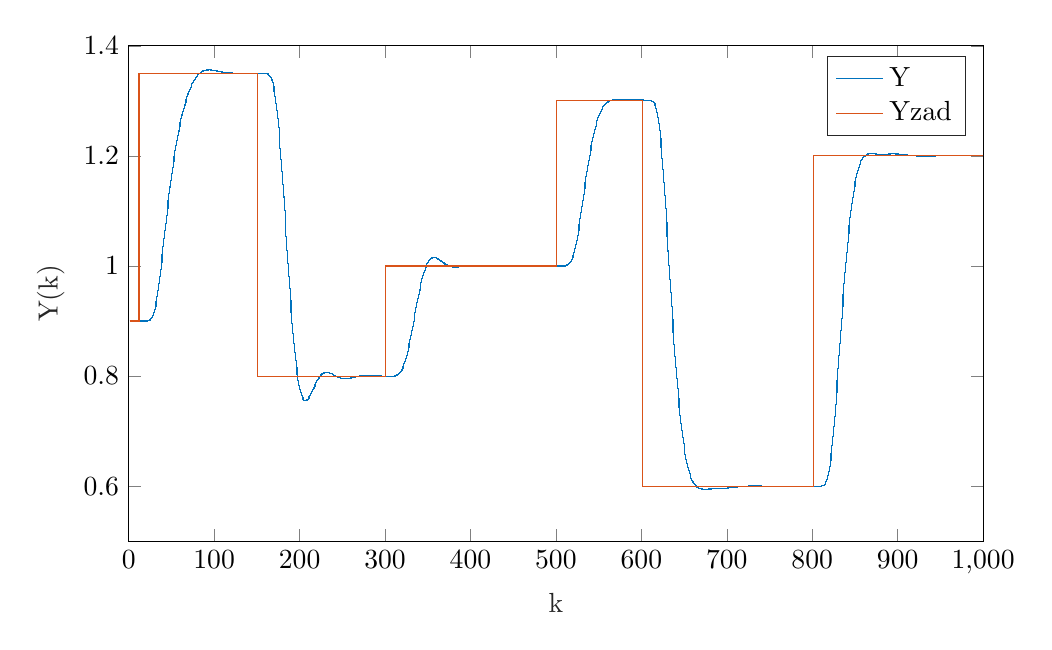
\begin{tikzpicture}

\begin{axis}[%
width=4.272in,
height=2.477in,
at={(0.717in,0.437in)},
scale only axis,
xmin=0,
xmax=1000,
xlabel style={font=\color{white!15!black}},
xlabel={k},
ymin=0.5,
ymax=1.4,
ylabel style={font=\color{white!15!black}},
ylabel={Y(k)},
axis background/.style={fill=white},
legend style={legend cell align=left, align=left, draw=white!15!black}
]
\addplot[const plot, color=mycolor1] table[row sep=crcr] {%
1	0.9\\
2	0.9\\
3	0.9\\
4	0.9\\
5	0.9\\
6	0.9\\
7	0.9\\
8	0.9\\
9	0.9\\
10	0.9\\
11	0.9\\
12	0.9\\
13	0.9\\
14	0.9\\
15	0.9\\
16	0.9\\
17	0.9\\
18	0.9\\
19	0.9\\
20	0.9\\
21	0.9\\
22	0.9003968325\\
23	0.90110505465075\\
24	0.901851548804444\\
25	0.902926732649044\\
26	0.9045740507257\\
27	0.906995673734868\\
28	0.910357581452216\\
29	0.91479409195594\\
30	0.92041189372332\\
31	0.927293631597811\\
32	0.935481917271842\\
33	0.944987479442384\\
34	0.955752143856375\\
35	0.967585143897724\\
36	0.980245690511738\\
37	0.993524900254613\\
38	1.00724220273058\\
39	1.02124212187654\\
40	1.03539139393444\\
41	1.04957638853821\\
42	1.06370080258905\\
43	1.07768359953247\\
44	1.09145716931113\\
45	1.10496568667539\\
46	1.11816364771215\\
47	1.13101456642337\\
48	1.1434898149686\\
49	1.15556759279779\\
50	1.16723201135847\\
51	1.17847228237882\\
52	1.18928199891931\\
53	1.19965849946121\\
54	1.20960230627283\\
55	1.21911663017192\\
56	1.22820693459549\\
57	1.23688055260421\\
58	1.24514635109392\\
59	1.25301443706996\\
60	1.26049590136546\\
61	1.26760259565856\\
62	1.27434693907117\\
63	1.28074174608457\\
64	1.28679954411603\\
65	1.29253204733993\\
66	1.29795023797434\\
67	1.3030644413896\\
68	1.3078843950437\\
69	1.31241931135295\\
70	1.31667793468543\\
71	1.32066859272397\\
72	1.32439924248811\\
73	1.32787751157148\\
74	1.33111076093811\\
75	1.33410618724198\\
76	1.33687093004876\\
77	1.33941215850932\\
78	1.34173714007823\\
79	1.34385329361559\\
80	1.34576822897515\\
81	1.34748977496456\\
82	1.34902599736423\\
83	1.3503852084965\\
84	1.35157596840274\\
85	1.35260707550363\\
86	1.35348754538761\\
87	1.35422657910142\\
88	1.3548335232566\\
89	1.35531782394082\\
90	1.35568897613632\\
91	1.35595647009444\\
92	1.35612973589315\\
93	1.35621808720922\\
94	1.35623066522872\\
95	1.35617638368734\\
96	1.35606387616748\\
97	1.35590144675004\\
98	1.35569702492415\\
99	1.35545812544111\\
100	1.35519181361515\\
101	1.35490467641866\\
102	1.35460279958943\\
103	1.35429175085935\\
104	1.35397656932081\\
105	1.35366176085724\\
106	1.35335129946519\\
107	1.35304863419235\\
108	1.35275670132403\\
109	1.35247794137879\\
110	1.35221432042028\\
111	1.35196735515504\\
112	1.35173814126113\\
113	1.35152738437876\\
114	1.35133543318901\\
115	1.35116231400986\\
116	1.35100776635043\\
117	1.35087127888471\\
118	1.35075212533525\\
119	1.35064939979385\\
120	1.35056205104808\\
121	1.35048891552808\\
122	1.35042874853686\\
123	1.35038025347687\\
124	1.35034210883664\\
125	1.35031299275196\\
126	1.35029160500585\\
127	1.3502766863805\\
128	1.35026703532044\\
129	1.35026152190965\\
130	1.35025909920554\\
131	1.35025881200833\\
132	1.35025980317699\\
133	1.35026131763001\\
134	1.3502627041929\\
135	1.35026341547329\\
136	1.35026300595865\\
137	1.35026112854246\\
138	1.35025752969034\\
139	1.35025204346031\\
140	1.35024458458987\\
141	1.35023514085807\\
142	1.35022376492329\\
143	1.35021056582744\\
144	1.35019570034494\\
145	1.35017936434093\\
146	1.35016178428769\\
147	1.35014320907172\\
148	1.35012390220676\\
149	1.35010413455032\\
150	1.35008417760403\\
151	1.35006429746031\\
152	1.35004474944139\\
153	1.35002577346057\\
154	1.35000759012025\\
155	1.34999039754741\\
156	1.34997436895457\\
157	1.34995965090253\\
158	1.34994636223132\\
159	1.34993459361745\\
160	1.34992440770813\\
161	1.34951889923522\\
162	1.34880333328902\\
163	1.34801637133565\\
164	1.34680623564434\\
165	1.34487818982496\\
166	1.34198761101855\\
167	1.33793381210464\\
168	1.33255453756716\\
169	1.32572106414159\\
170	1.31733384413307\\
171	1.30733781596696\\
172	1.29571365605078\\
173	1.2824452175893\\
174	1.26753853904809\\
175	1.25104365760431\\
176	1.23304727100621\\
177	1.21366635998876\\
178	1.19304265516873\\
179	1.1713378458413\\
180	1.14872944006864\\
181	1.12540626923593\\
182	1.10156388099674\\
183	1.07740205013679\\
184	1.05312296740804\\
185	1.02892759572966\\
186	1.00501147782133\\
187	0.98156127181985\\
188	0.958751911430767\\
189	0.936744301032577\\
190	0.915683468219405\\
191	0.895697151551403\\
192	0.87689483720541\\
193	0.859367140555324\\
194	0.843185398442461\\
195	0.828401526929037\\
196	0.815048252072926\\
197	0.803139700616667\\
198	0.792672284955702\\
199	0.783625826910249\\
200	0.775964873487657\\
201	0.769640163035288\\
202	0.764590200971363\\
203	0.760742909007944\\
204	0.758017323223758\\
205	0.75632531988144\\
206	0.755573340172202\\
207	0.755664080816826\\
208	0.75649812124768\\
209	0.757975463734339\\
210	0.759996967501476\\
211	0.762465661879657\\
212	0.765287927215516\\
213	0.768374535670495\\
214	0.771641546661306\\
215	0.775011053627311\\
216	0.778411780963361\\
217	0.781779532677985\\
218	0.785057497075944\\
219	0.78819641406661\\
220	0.791154613532383\\
221	0.793897934635967\\
222	0.79639953705089\\
223	0.798639615895301\\
224	0.800605032685999\\
225	0.802288874976543\\
226	0.803689957519954\\
227	0.804812277764049\\
228	0.805664438217677\\
229	0.80625904773855\\
230	0.806612113128949\\
231	0.80674243162307\\
232	0.806670993941009\\
233	0.806420406597751\\
234	0.806014341115425\\
235	0.805477016712229\\
236	0.804832721946634\\
237	0.80410537969662\\
238	0.803318158769883\\
239	0.802493134391884\\
240	0.801650998821049\\
241	0.800810822407754\\
242	0.799989864555977\\
243	0.799203433271251\\
244	0.798464791291063\\
245	0.79778510619742\\
246	0.797173441408183\\
247	0.796636784534522\\
248	0.796180109276034\\
249	0.795806466800069\\
250	0.795517102413963\\
251	0.795311593282831\\
252	0.795188002965221\\
253	0.795143048627405\\
254	0.795172276946966\\
255	0.795270244919908\\
256	0.795430702034841\\
257	0.795646770564863\\
258	0.795911121044516\\
259	0.796216140337837\\
260	0.796554090056421\\
261	0.796917253446428\\
262	0.797298069223946\\
263	0.797689251192951\\
264	0.798083892823816\\
265	0.79847555629814\\
266	0.798858345833424\\
267	0.799226965385318\\
268	0.799576761083186\\
269	0.799903748984284\\
270	0.800204628931693\\
271	0.800476785470349\\
272	0.800718276913917\\
273	0.800927813763172\\
274	0.801104727754768\\
275	0.801248932869047\\
276	0.801360879648473\\
277	0.801441504176269\\
278	0.801492173040124\\
279	0.801514625560706\\
280	0.801510914501775\\
281	0.801483346400498\\
282	0.801434422565709\\
283	0.801366781691079\\
284	0.801283144921891\\
285	0.80118626410091\\
286	0.80107887380304\\
287	0.80096364765217\\
288	0.800843159298981\\
289	0.800719848327149\\
290	0.800595991249099\\
291	0.800473677652468\\
292	0.800354791466003\\
293	0.800240997229543\\
294	0.800133731177851\\
295	0.800034196882735\\
296	0.799943365142501\\
297	0.799861977762359\\
298	0.799790554833885\\
299	0.799729405095798\\
300	0.799678638941685\\
301	0.799638183632529\\
302	0.799607800272158\\
303	0.799587102111522\\
304	0.799575573762118\\
305	0.79957259091919\\
306	0.799577440220629\\
307	0.799589338896979\\
308	0.799607453900748\\
309	0.799630920238458\\
310	0.799658858265823\\
311	0.800087252030063\\
312	0.800829896899739\\
313	0.801526913554124\\
314	0.802314448958003\\
315	0.803306971242467\\
316	0.804599897685075\\
317	0.80627193853803\\
318	0.808387185421943\\
319	0.810996970220403\\
320	0.814141517893137\\
321	0.817832237576928\\
322	0.822058342893119\\
323	0.82682333598127\\
324	0.832134339197458\\
325	0.837981296502411\\
326	0.844339788339714\\
327	0.851173479010461\\
328	0.858436240883071\\
329	0.866073994644319\\
330	0.874026300243561\\
331	0.882228655782662\\
332	0.890615216678407\\
333	0.899119386465001\\
334	0.907673219149908\\
335	0.916208290634322\\
336	0.924657350987353\\
337	0.932955694514448\\
338	0.941042287608186\\
339	0.948860689023248\\
340	0.956359792560657\\
341	0.963494373316752\\
342	0.970225388345921\\
343	0.976520118682778\\
344	0.982352309401972\\
345	0.98770229142151\\
346	0.992556980678792\\
347	0.996909733881368\\
348	1.00076008658177\\
349	1.00411339535527\\
350	1.00698040247153\\
351	1.00937674072753\\
352	1.01132239913817\\
353	1.01284116803809\\
354	1.0139600704795\\
355	1.01470878044002\\
356	1.01511903420175\\
357	1.01522404704477\\
358	1.01505794707236\\
359	1.0146552357442\\
360	1.01405028282807\\
361	1.01327686182708\\
362	1.01236773018765\\
363	1.01135425681932\\
364	1.01026609835369\\
365	1.00913092530819\\
366	1.0079741990589\\
367	1.00681899971261\\
368	1.0056859039023\\
369	1.00459291058741\\
370	1.00355541218626\\
371	1.00258620777425\\
372	1.00169555464129\\
373	1.00089125422008\\
374	1.00017876824074\\
375	0.999561360866317\\
376	0.99904026247886\\
377	0.99861485074555\\
378	0.998282844636035\\
379	0.998040507192143\\
380	0.997882853054599\\
381	0.997803857012575\\
382	0.99779666014669\\
383	0.997853770470491\\
384	0.997967255326939\\
385	0.998128923157442\\
386	0.998330492628963\\
387	0.99856374747751\\
388	0.998820675798544\\
389	0.99909359287906\\
390	0.99937524701533\\
391	0.999658908088884\\
392	0.999938438976968\\
393	1.00020835014948\\
394	1.00046383805041\\
395	1.00070080807695\\
396	1.0009158831536\\
397	1.00110639905052\\
398	1.00127038771589\\
399	1.00140654998108\\
400	1.00151421905542\\
401	1.00159331625788\\
402	1.00164430043515\\
403	1.00166811249474\\
404	1.00166611643787\\
405	1.00164003821447\\
406	1.00159190364311\\
407	1.00152397654534\\
408	1.00143869813951\\
409	1.00133862862597\\
410	1.00122639177664\\
411	1.00110462321982\\
412	1.00097592298746\\
413	1.00084281277039\\
414	1.00070769820757\\
415	1.00057283642144\\
416	1.00044030890337\\
417	1.00031199975319\\
418	1.00018957918462\\
419	1.00007449212675\\
420	0.999967951678888\\
421	0.999870937114806\\
422	0.999784196080508\\
423	0.999708250589163\\
424	0.99964340638599\\
425	0.999589765235247\\
426	0.999547239670111\\
427	0.99951556974366\\
428	0.999494341324697\\
429	0.99948300549489\\
430	0.999480898622941\\
431	0.999487262716258\\
432	0.999501265680006\\
433	0.99952202114661\\
434	0.999548607574855\\
435	0.999580086355753\\
436	0.999615518701678\\
437	0.999653981134935\\
438	0.999694579431357\\
439	0.999736460913058\\
440	0.999778825021436\\
441	0.999820932136559\\
442	0.999862110641679\\
443	0.999901762261401\\
444	0.999939365728923\\
445	0.999974478861247\\
446	1.0000067391416\\
447	1.00003586292502\\
448	1.00006164339664\\
449	1.00008394742205\\
450	1.0001027114364\\
451	1.0001179365222\\
452	1.0001296828272\\
453	1.00013806347171\\
454	1.00014323809091\\
455	1.00014540615114\\
456	1.00014480017174\\
457	1.0001416789738\\
458	1.00013632106689\\
459	1.0001290182729\\
460	1.00012006967369\\
461	1.00010977595652\\
462	1.00009843421817\\
463	1.00008633327581\\
464	1.00007374952002\\
465	1.00006094333331\\
466	1.0000481560859\\
467	1.00003560770982\\
468	1.00002349484263\\
469	1.00001198952323\\
470	1.00000123841427\\
471	0.999991362519225\\
472	0.999982457356436\\
473	0.999974593547984\\
474	0.999967817777953\\
475	0.999962154072194\\
476	0.999957605350476\\
477	0.999954155201463\\
478	0.999951769831483\\
479	0.999950400139309\\
480	0.999949983871121\\
481	0.99995044781243\\
482	0.999951709976786\\
483	0.999953681754603\\
484	0.999956269989249\\
485	0.999959378951586\\
486	0.999962912188326\\
487	0.999966774223801\\
488	0.999970872098985\\
489	0.999975116735722\\
490	0.999979424118093\\
491	0.99998371628665\\
492	0.999987922144747\\
493	0.999991978079466\\
494	0.99999582840252\\
495	0.99999942561911\\
496	1.00000273053496\\
497	1.00000571221353\\
498	1.00000834779705\\
499	1.00001062220599\\
500	1.00001252773249\\
501	1.00001406354371\\
502	1.00001523511121\\
503	1.00001605358234\\
504	1.00001653510923\\
505	1.00001670015035\\
506	1.0000165727588\\
507	1.00001617987058\\
508	1.00001555060467\\
509	1.00001471558604\\
510	1.00001370630078\\
511	1.00040938687002\\
512	1.00111634385559\\
513	1.00180990053873\\
514	1.00268843571159\\
515	1.00391849735183\\
516	1.00563865417243\\
517	1.00796293117229\\
518	1.01098387147904\\
519	1.01477526263231\\
520	1.01939456170907\\
521	1.02486587497793\\
522	1.03118719384104\\
523	1.03836576030038\\
524	1.04640501110105\\
525	1.0552810410956\\
526	1.06488021579298\\
527	1.07502937461854\\
528	1.08557859040799\\
529	1.09639853937936\\
530	1.10737814558263\\
531	1.11842247249576\\
532	1.12945083707684\\
533	1.14039512397285\\
534	1.15119606058873\\
535	1.16179467306295\\
536	1.17213167238055\\
537	1.18215529846576\\
538	1.19182363951412\\
539	1.20110321653843\\
540	1.20996775970649\\
541	1.21839715135172\\
542	1.22637651371243\\
543	1.23389542224359\\
544	1.24094733502383\\
545	1.24752956493031\\
546	1.25364362999629\\
547	1.25929521154068\\
548	1.26449360774086\\
549	1.26925112252173\\
550	1.27358255346119\\
551	1.27750476271623\\
552	1.28103631742981\\
553	1.28419718817999\\
554	1.28700849064702\\
555	1.28949223585751\\
556	1.29167104761675\\
557	1.29356785069549\\
558	1.29520557374751\\
559	1.29660689429689\\
560	1.29779402483979\\
561	1.29878853239093\\
562	1.29961118523015\\
563	1.30028182178583\\
564	1.30081923782027\\
565	1.30124109040346\\
566	1.30156382069269\\
567	1.30180259917413\\
568	1.30197129465071\\
569	1.30208246487385\\
570	1.30214736548998\\
571	1.30217597436986\\
572	1.30217702901752\\
573	1.30215807525415\\
574	1.30212552575333\\
575	1.30208472721385\\
576	1.30204003488983\\
577	1.30199489289285\\
578	1.30195191841996\\
579	1.3019129880756\\
580	1.30187932468478\\
581	1.30185158325917\\
582	1.30182993499384\\
583	1.30181414833495\\
584	1.30180366628157\\
585	1.30179767918116\\
586	1.30179519237017\\
587	1.30179508812259\\
588	1.30179618150869\\
589	1.3017972699183\\
590	1.30179717614454\\
591	1.3017947850439\\
592	1.30178907388725\\
593	1.30177913659974\\
594	1.30176420215849\\
595	1.30174364748047\\
596	1.30171700518821\\
597	1.30168396668942\\
598	1.30164438104379\\
599	1.30159825011591\\
600	1.30154572052602\\
601	1.30148707291275\\
602	1.30142270901472\\
603	1.30135313706407\\
604	1.30127895596416\\
605	1.30120083869815\\
606	1.30111951538432\\
607	1.30103575635944\\
608	1.30095035563282\\
609	1.30086411501358\\
610	1.30077782917065\\
611	1.30029530496667\\
612	1.29950244188333\\
613	1.29858697269979\\
614	1.29710576065386\\
615	1.29468780983826\\
616	1.29102548178189\\
617	1.28586666380651\\
618	1.27900779241308\\
619	1.27028764440437\\
620	1.25958181700166\\
621	1.24681700777077\\
622	1.23196135693652\\
623	1.2149935713611\\
624	1.19592550639499\\
625	1.17491223308447\\
626	1.15229778220868\\
627	1.12847426818706\\
628	1.10378096176539\\
629	1.07851028303056\\
630	1.05291316834887\\
631	1.02720387360807\\
632	1.00156427011363\\
633	0.976147684030359\\
634	0.951091932865076\\
635	0.926534189279658\\
636	0.902604680696242\\
637	0.879413695440342\\
638	0.857050192325861\\
639	0.835584891327783\\
640	0.815072942016301\\
641	0.795556225465445\\
642	0.777065338265068\\
643	0.759621301048111\\
644	0.743236564246909\\
645	0.727914801800709\\
646	0.713650434135868\\
647	0.700429163687804\\
648	0.688229250977027\\
649	0.677022772194998\\
650	0.666776669450702\\
651	0.657453627862084\\
652	0.649012808347463\\
653	0.641410460419988\\
654	0.634600457839202\\
655	0.628534843868629\\
656	0.623164450182839\\
657	0.618439548302297\\
658	0.614310447724342\\
659	0.610728005041552\\
660	0.607644052578591\\
661	0.605011762067602\\
662	0.602785955903782\\
663	0.600923376062281\\
664	0.599382917648758\\
665	0.598125828015592\\
666	0.597115865478575\\
667	0.596319410936442\\
668	0.595705531912505\\
669	0.595246004305127\\
670	0.594915298420306\\
671	0.594690534780794\\
672	0.594551413965632\\
673	0.59448012376013\\
674	0.594461226191505\\
675	0.594481526756459\\
676	0.594529928484425\\
677	0.594597274160046\\
678	0.594676180431389\\
679	0.594760867364182\\
680	0.594846986509326\\
681	0.594931450052203\\
682	0.595012263222892\\
683	0.595088361859101\\
684	0.595159456801897\\
685	0.595225886634035\\
686	0.595288480092274\\
687	0.595348429254399\\
688	0.595407174317053\\
689	0.595466300482387\\
690	0.595527447201913\\
691	0.595592229799617\\
692	0.595662173308058\\
693	0.595738658190722\\
694	0.595822877482975\\
695	0.595915804757238\\
696	0.596018172204116\\
697	0.596130458023276\\
698	0.596252882240983\\
699	0.596385410018751\\
700	0.596527761488751\\
701	0.59667942714332\\
702	0.596839687814509\\
703	0.59700763830213\\
704	0.597182213743416\\
705	0.597362217862657\\
706	0.597546352294202\\
707	0.597733246235749\\
708	0.597921485759412\\
709	0.598109642183802\\
710	0.598296298989114\\
711	0.598480076837217\\
712	0.59865965633843\\
713	0.598833798284704\\
714	0.599001361144349\\
715	0.599161315685303\\
716	0.599312756661364\\
717	0.599454911558148\\
718	0.599587146452061\\
719	0.599708969085893\\
720	0.599820029308329\\
721	0.599920117061697\\
722	0.600009158132504\\
723	0.60008720790297\\
724	0.600154443358984\\
725	0.600211153620972\\
726	0.600257729269507\\
727	0.600294650737418\\
728	0.600322476035205\\
729	0.600341828067307\\
730	0.600353381783611\\
731	0.600357851394269\\
732	0.600355977856853\\
733	0.600348516823772\\
734	0.600336227215196\\
735	0.600319860559061\\
736	0.600300151215525\\
737	0.600277807578992\\
738	0.600253504326954\\
739	0.600227875761784\\
740	0.600201510269595\\
741	0.600174945899655\\
742	0.600148667048844\\
743	0.600123102218444\\
744	0.600098622795336\\
745	0.600075542796498\\
746	0.600054119504641\\
747	0.60003455491389\\
748	0.60001699789755\\
749	0.600001547005246\\
750	0.599988253793833\\
751	0.599977126595481\\
752	0.599968134627041\\
753	0.59996121234702\\
754	0.59995626397012\\
755	0.599953168054114\\
756	0.599951782079693\\
757	0.599951946950578\\
758	0.599953491348562\\
759	0.599956235885924\\
760	0.599959997005831\\
761	0.599964590589559\\
762	0.599969835237675\\
763	0.599975555200391\\
764	0.599981582940186\\
765	0.599987761317235\\
766	0.599993945395198\\
767	0.600000003871361\\
768	0.600005820140961\\
769	0.600011293010712\\
770	0.600016337081039\\
771	0.600020882820316\\
772	0.600024876357481\\
773	0.600028279021781\\
774	0.600031066660103\\
775	0.600033228763376\\
776	0.600034767433985\\
777	0.600035696225979\\
778	0.600036038889217\\
779	0.600035828047462\\
780	0.600035103838924\\
781	0.600033912545884\\
782	0.600032305237853\\
783	0.600030336450394\\
784	0.600028062919133\\
785	0.60002554238589\\
786	0.600022832491118\\
787	0.60001998976415\\
788	0.600017068720083\\
789	0.600014121069528\\
790	0.60001119504502\\
791	0.600008334845534\\
792	0.600005580198432\\
793	0.600002966036214\\
794	0.600000522283721\\
795	0.599998273749941\\
796	0.599996240117256\\
797	0.599994436019977\\
798	0.599992871203143\\
799	0.599991550752008\\
800	0.59999047538224\\
801	0.599989641780678\\
802	0.599989042986521\\
803	0.599988668802976\\
804	0.599988506229756\\
805	0.599988539907271\\
806	0.599988752563946\\
807	0.599989125458765\\
808	0.599989638811934\\
809	0.599990272217311\\
810	0.599991005031156\\
811	0.600388650057562\\
812	0.60109774693152\\
813	0.601896748159271\\
814	0.603168121212745\\
815	0.605232217684207\\
816	0.608354820198316\\
817	0.61275387256598\\
818	0.618605476291989\\
819	0.62604922840339\\
820	0.635192968199196\\
821	0.646097818489643\\
822	0.658787249924379\\
823	0.673279080671453\\
824	0.689565266689302\\
825	0.707589940697784\\
826	0.72713446457966\\
827	0.747853988948476\\
828	0.769434371273039\\
829	0.791604494552311\\
830	0.814131355019799\\
831	0.836815664872935\\
832	0.859487918598574\\
833	0.882004876444571\\
834	0.904238695684769\\
835	0.926060237922586\\
836	0.947340357661263\\
837	0.967965091722119\\
838	0.987841316522553\\
839	1.0068944779348\\
840	1.02506591488485\\
841	1.04231054442164\\
842	1.05859486105224\\
843	1.07389520909596\\
844	1.08819666543733\\
845	1.1014931491119\\
846	1.11378815029982\\
847	1.12509458769098\\
848	1.13543363434851\\
849	1.14483334429767\\
850	1.15332746639235\\
851	1.16095444771135\\
852	1.16775659620422\\
853	1.17377937693106\\
854	1.17907080215597\\
855	1.1836808307137\\
856	1.18766069386918\\
857	1.19106216511983\\
858	1.19393686673454\\
859	1.19633567187569\\
860	1.19830820387889\\
861	1.19990241649128\\
862	1.20116424035816\\
863	1.2021372837453\\
864	1.20286257859648\\
865	1.20337836889993\\
866	1.20371994611261\\
867	1.2039195391791\\
868	1.20400626124261\\
869	1.20400610796582\\
870	1.2039419995818\\
871	1.20383385948778\\
872	1.2036987236111\\
873	1.2035508759748\\
874	1.20340200680221\\
875	1.20326138997741\\
876	1.20313607651004\\
877	1.20303109999871\\
878	1.20294968957644\\
879	1.20289348591148\\
880	1.20286275639048\\
881	1.20285660625548\\
882	1.20287318300823\\
883	1.20290987181465\\
884	1.20296347996343\\
885	1.2030304086929\\
886	1.20310681094963\\
887	1.20318873393483\\
888	1.20327224564506\\
889	1.20335354498642\\
890	1.20342905538578\\
891	1.20349550211422\\
892	1.20354997377777\\
893	1.20358996862898\\
894	1.20361342652154\\
895	1.20361874747566\\
896	1.20360479794724\\
897	1.20357090599802\\
898	1.20351684664133\\
899	1.20344281868494\\
900	1.20334941440898\\
901	1.20323758340745\\
902	1.20310859188937\\
903	1.20296397868653\\
904	1.20280550914981\\
905	1.20263512803931\\
906	1.2024549124254\\
907	1.20226702552041\\
908	1.20207367225652\\
909	1.20187705731565\\
910	1.20167934620581\\
911	1.20148262986666\\
912	1.201288893178\\
913	1.20109998763908\\
914	1.20091760838659\\
915	1.20074327562482\\
916	1.20057832045494\\
917	1.200423875011\\
918	1.20028086674055\\
919	1.20015001660639\\
920	1.20003184093447\\
921	1.19992665659092\\
922	1.19983458913817\\
923	1.19975558359666\\
924	1.1996894174234\\
925	1.19963571531159\\
926	1.19959396541634\\
927	1.1995635366188\\
928	1.19954369645458\\
929	1.19953362935164\\
930	1.19953245484586\\
931	1.19953924547042\\
932	1.19955304404509\\
933	1.19957288012405\\
934	1.1995977853949\\
935	1.19962680785622\\
936	1.19965902463557\\
937	1.19969355334433\\
938	1.19972956189858\\
939	1.19976627676725\\
940	1.1998029896378\\
941	1.19983906251768\\
942	1.19987393131392\\
943	1.19990710795575\\
944	1.19993818114369\\
945	1.19996681582489\\
946	1.19999275150757\\
947	1.2000157995371\\
948	1.20003583946385\\
949	1.20005281463692\\
950	1.20006672715987\\
951	1.20007763234356\\
952	1.20008563278877\\
953	1.20009087222583\\
954	1.20009352923226\\
955	1.20009381094132\\
956	1.20009194684477\\
957	1.20008818278318\\
958	1.20008277520624\\
959	1.20007598577364\\
960	1.20006807635612\\
961	1.2000593044841\\
962	1.20004991928013\\
963	1.20004015790023\\
964	1.20003024249866\\
965	1.2000203777206\\
966	1.2000107487183\\
967	1.20000151967768\\
968	1.19999283283525\\
969	1.19998480795856\\
970	1.19997754225813\\
971	1.19997111069432\\
972	1.19996556663914\\
973	1.19996094285058\\
974	1.19995725271548\\
975	1.19995449171614\\
976	1.19995263907622\\
977	1.19995165954222\\
978	1.19995150525822\\
979	1.19995211769391\\
980	1.19995342958837\\
981	1.19995536687497\\
982	1.19995785055642\\
983	1.19996079850207\\
984	1.19996412714364\\
985	1.19996775304935\\
986	1.19997159435988\\
987	1.19997557207384\\
988	1.19997961117361\\
989	1.19998364158628\\
990	1.1999875989774\\
991	1.1999914253784\\
992	1.19999506965136\\
993	1.19999848779709\\
994	1.20000164311476\\
995	1.20000450622315\\
996	1.20000705495485\\
997	1.20000927413629\\
998	1.20001115526697\\
999	1.20001269611206\\
1000	1.20001390022257\\
};
\addlegendentry{Y}

\addplot[const plot, color=mycolor2] table[row sep=crcr] {%
1	0.9\\
2	0.9\\
3	0.9\\
4	0.9\\
5	0.9\\
6	0.9\\
7	0.9\\
8	0.9\\
9	0.9\\
10	0.9\\
11	0.9\\
12	1.35\\
13	1.35\\
14	1.35\\
15	1.35\\
16	1.35\\
17	1.35\\
18	1.35\\
19	1.35\\
20	1.35\\
21	1.35\\
22	1.35\\
23	1.35\\
24	1.35\\
25	1.35\\
26	1.35\\
27	1.35\\
28	1.35\\
29	1.35\\
30	1.35\\
31	1.35\\
32	1.35\\
33	1.35\\
34	1.35\\
35	1.35\\
36	1.35\\
37	1.35\\
38	1.35\\
39	1.35\\
40	1.35\\
41	1.35\\
42	1.35\\
43	1.35\\
44	1.35\\
45	1.35\\
46	1.35\\
47	1.35\\
48	1.35\\
49	1.35\\
50	1.35\\
51	1.35\\
52	1.35\\
53	1.35\\
54	1.35\\
55	1.35\\
56	1.35\\
57	1.35\\
58	1.35\\
59	1.35\\
60	1.35\\
61	1.35\\
62	1.35\\
63	1.35\\
64	1.35\\
65	1.35\\
66	1.35\\
67	1.35\\
68	1.35\\
69	1.35\\
70	1.35\\
71	1.35\\
72	1.35\\
73	1.35\\
74	1.35\\
75	1.35\\
76	1.35\\
77	1.35\\
78	1.35\\
79	1.35\\
80	1.35\\
81	1.35\\
82	1.35\\
83	1.35\\
84	1.35\\
85	1.35\\
86	1.35\\
87	1.35\\
88	1.35\\
89	1.35\\
90	1.35\\
91	1.35\\
92	1.35\\
93	1.35\\
94	1.35\\
95	1.35\\
96	1.35\\
97	1.35\\
98	1.35\\
99	1.35\\
100	1.35\\
101	1.35\\
102	1.35\\
103	1.35\\
104	1.35\\
105	1.35\\
106	1.35\\
107	1.35\\
108	1.35\\
109	1.35\\
110	1.35\\
111	1.35\\
112	1.35\\
113	1.35\\
114	1.35\\
115	1.35\\
116	1.35\\
117	1.35\\
118	1.35\\
119	1.35\\
120	1.35\\
121	1.35\\
122	1.35\\
123	1.35\\
124	1.35\\
125	1.35\\
126	1.35\\
127	1.35\\
128	1.35\\
129	1.35\\
130	1.35\\
131	1.35\\
132	1.35\\
133	1.35\\
134	1.35\\
135	1.35\\
136	1.35\\
137	1.35\\
138	1.35\\
139	1.35\\
140	1.35\\
141	1.35\\
142	1.35\\
143	1.35\\
144	1.35\\
145	1.35\\
146	1.35\\
147	1.35\\
148	1.35\\
149	1.35\\
150	1.35\\
151	0.8\\
152	0.8\\
153	0.8\\
154	0.8\\
155	0.8\\
156	0.8\\
157	0.8\\
158	0.8\\
159	0.8\\
160	0.8\\
161	0.8\\
162	0.8\\
163	0.8\\
164	0.8\\
165	0.8\\
166	0.8\\
167	0.8\\
168	0.8\\
169	0.8\\
170	0.8\\
171	0.8\\
172	0.8\\
173	0.8\\
174	0.8\\
175	0.8\\
176	0.8\\
177	0.8\\
178	0.8\\
179	0.8\\
180	0.8\\
181	0.8\\
182	0.8\\
183	0.8\\
184	0.8\\
185	0.8\\
186	0.8\\
187	0.8\\
188	0.8\\
189	0.8\\
190	0.8\\
191	0.8\\
192	0.8\\
193	0.8\\
194	0.8\\
195	0.8\\
196	0.8\\
197	0.8\\
198	0.8\\
199	0.8\\
200	0.8\\
201	0.8\\
202	0.8\\
203	0.8\\
204	0.8\\
205	0.8\\
206	0.8\\
207	0.8\\
208	0.8\\
209	0.8\\
210	0.8\\
211	0.8\\
212	0.8\\
213	0.8\\
214	0.8\\
215	0.8\\
216	0.8\\
217	0.8\\
218	0.8\\
219	0.8\\
220	0.8\\
221	0.8\\
222	0.8\\
223	0.8\\
224	0.8\\
225	0.8\\
226	0.8\\
227	0.8\\
228	0.8\\
229	0.8\\
230	0.8\\
231	0.8\\
232	0.8\\
233	0.8\\
234	0.8\\
235	0.8\\
236	0.8\\
237	0.8\\
238	0.8\\
239	0.8\\
240	0.8\\
241	0.8\\
242	0.8\\
243	0.8\\
244	0.8\\
245	0.8\\
246	0.8\\
247	0.8\\
248	0.8\\
249	0.8\\
250	0.8\\
251	0.8\\
252	0.8\\
253	0.8\\
254	0.8\\
255	0.8\\
256	0.8\\
257	0.8\\
258	0.8\\
259	0.8\\
260	0.8\\
261	0.8\\
262	0.8\\
263	0.8\\
264	0.8\\
265	0.8\\
266	0.8\\
267	0.8\\
268	0.8\\
269	0.8\\
270	0.8\\
271	0.8\\
272	0.8\\
273	0.8\\
274	0.8\\
275	0.8\\
276	0.8\\
277	0.8\\
278	0.8\\
279	0.8\\
280	0.8\\
281	0.8\\
282	0.8\\
283	0.8\\
284	0.8\\
285	0.8\\
286	0.8\\
287	0.8\\
288	0.8\\
289	0.8\\
290	0.8\\
291	0.8\\
292	0.8\\
293	0.8\\
294	0.8\\
295	0.8\\
296	0.8\\
297	0.8\\
298	0.8\\
299	0.8\\
300	0.8\\
301	1\\
302	1\\
303	1\\
304	1\\
305	1\\
306	1\\
307	1\\
308	1\\
309	1\\
310	1\\
311	1\\
312	1\\
313	1\\
314	1\\
315	1\\
316	1\\
317	1\\
318	1\\
319	1\\
320	1\\
321	1\\
322	1\\
323	1\\
324	1\\
325	1\\
326	1\\
327	1\\
328	1\\
329	1\\
330	1\\
331	1\\
332	1\\
333	1\\
334	1\\
335	1\\
336	1\\
337	1\\
338	1\\
339	1\\
340	1\\
341	1\\
342	1\\
343	1\\
344	1\\
345	1\\
346	1\\
347	1\\
348	1\\
349	1\\
350	1\\
351	1\\
352	1\\
353	1\\
354	1\\
355	1\\
356	1\\
357	1\\
358	1\\
359	1\\
360	1\\
361	1\\
362	1\\
363	1\\
364	1\\
365	1\\
366	1\\
367	1\\
368	1\\
369	1\\
370	1\\
371	1\\
372	1\\
373	1\\
374	1\\
375	1\\
376	1\\
377	1\\
378	1\\
379	1\\
380	1\\
381	1\\
382	1\\
383	1\\
384	1\\
385	1\\
386	1\\
387	1\\
388	1\\
389	1\\
390	1\\
391	1\\
392	1\\
393	1\\
394	1\\
395	1\\
396	1\\
397	1\\
398	1\\
399	1\\
400	1\\
401	1\\
402	1\\
403	1\\
404	1\\
405	1\\
406	1\\
407	1\\
408	1\\
409	1\\
410	1\\
411	1\\
412	1\\
413	1\\
414	1\\
415	1\\
416	1\\
417	1\\
418	1\\
419	1\\
420	1\\
421	1\\
422	1\\
423	1\\
424	1\\
425	1\\
426	1\\
427	1\\
428	1\\
429	1\\
430	1\\
431	1\\
432	1\\
433	1\\
434	1\\
435	1\\
436	1\\
437	1\\
438	1\\
439	1\\
440	1\\
441	1\\
442	1\\
443	1\\
444	1\\
445	1\\
446	1\\
447	1\\
448	1\\
449	1\\
450	1\\
451	1\\
452	1\\
453	1\\
454	1\\
455	1\\
456	1\\
457	1\\
458	1\\
459	1\\
460	1\\
461	1\\
462	1\\
463	1\\
464	1\\
465	1\\
466	1\\
467	1\\
468	1\\
469	1\\
470	1\\
471	1\\
472	1\\
473	1\\
474	1\\
475	1\\
476	1\\
477	1\\
478	1\\
479	1\\
480	1\\
481	1\\
482	1\\
483	1\\
484	1\\
485	1\\
486	1\\
487	1\\
488	1\\
489	1\\
490	1\\
491	1\\
492	1\\
493	1\\
494	1\\
495	1\\
496	1\\
497	1\\
498	1\\
499	1\\
500	1\\
501	1.3\\
502	1.3\\
503	1.3\\
504	1.3\\
505	1.3\\
506	1.3\\
507	1.3\\
508	1.3\\
509	1.3\\
510	1.3\\
511	1.3\\
512	1.3\\
513	1.3\\
514	1.3\\
515	1.3\\
516	1.3\\
517	1.3\\
518	1.3\\
519	1.3\\
520	1.3\\
521	1.3\\
522	1.3\\
523	1.3\\
524	1.3\\
525	1.3\\
526	1.3\\
527	1.3\\
528	1.3\\
529	1.3\\
530	1.3\\
531	1.3\\
532	1.3\\
533	1.3\\
534	1.3\\
535	1.3\\
536	1.3\\
537	1.3\\
538	1.3\\
539	1.3\\
540	1.3\\
541	1.3\\
542	1.3\\
543	1.3\\
544	1.3\\
545	1.3\\
546	1.3\\
547	1.3\\
548	1.3\\
549	1.3\\
550	1.3\\
551	1.3\\
552	1.3\\
553	1.3\\
554	1.3\\
555	1.3\\
556	1.3\\
557	1.3\\
558	1.3\\
559	1.3\\
560	1.3\\
561	1.3\\
562	1.3\\
563	1.3\\
564	1.3\\
565	1.3\\
566	1.3\\
567	1.3\\
568	1.3\\
569	1.3\\
570	1.3\\
571	1.3\\
572	1.3\\
573	1.3\\
574	1.3\\
575	1.3\\
576	1.3\\
577	1.3\\
578	1.3\\
579	1.3\\
580	1.3\\
581	1.3\\
582	1.3\\
583	1.3\\
584	1.3\\
585	1.3\\
586	1.3\\
587	1.3\\
588	1.3\\
589	1.3\\
590	1.3\\
591	1.3\\
592	1.3\\
593	1.3\\
594	1.3\\
595	1.3\\
596	1.3\\
597	1.3\\
598	1.3\\
599	1.3\\
600	1.3\\
601	0.6\\
602	0.6\\
603	0.6\\
604	0.6\\
605	0.6\\
606	0.6\\
607	0.6\\
608	0.6\\
609	0.6\\
610	0.6\\
611	0.6\\
612	0.6\\
613	0.6\\
614	0.6\\
615	0.6\\
616	0.6\\
617	0.6\\
618	0.6\\
619	0.6\\
620	0.6\\
621	0.6\\
622	0.6\\
623	0.6\\
624	0.6\\
625	0.6\\
626	0.6\\
627	0.6\\
628	0.6\\
629	0.6\\
630	0.6\\
631	0.6\\
632	0.6\\
633	0.6\\
634	0.6\\
635	0.6\\
636	0.6\\
637	0.6\\
638	0.6\\
639	0.6\\
640	0.6\\
641	0.6\\
642	0.6\\
643	0.6\\
644	0.6\\
645	0.6\\
646	0.6\\
647	0.6\\
648	0.6\\
649	0.6\\
650	0.6\\
651	0.6\\
652	0.6\\
653	0.6\\
654	0.6\\
655	0.6\\
656	0.6\\
657	0.6\\
658	0.6\\
659	0.6\\
660	0.6\\
661	0.6\\
662	0.6\\
663	0.6\\
664	0.6\\
665	0.6\\
666	0.6\\
667	0.6\\
668	0.6\\
669	0.6\\
670	0.6\\
671	0.6\\
672	0.6\\
673	0.6\\
674	0.6\\
675	0.6\\
676	0.6\\
677	0.6\\
678	0.6\\
679	0.6\\
680	0.6\\
681	0.6\\
682	0.6\\
683	0.6\\
684	0.6\\
685	0.6\\
686	0.6\\
687	0.6\\
688	0.6\\
689	0.6\\
690	0.6\\
691	0.6\\
692	0.6\\
693	0.6\\
694	0.6\\
695	0.6\\
696	0.6\\
697	0.6\\
698	0.6\\
699	0.6\\
700	0.6\\
701	0.6\\
702	0.6\\
703	0.6\\
704	0.6\\
705	0.6\\
706	0.6\\
707	0.6\\
708	0.6\\
709	0.6\\
710	0.6\\
711	0.6\\
712	0.6\\
713	0.6\\
714	0.6\\
715	0.6\\
716	0.6\\
717	0.6\\
718	0.6\\
719	0.6\\
720	0.6\\
721	0.6\\
722	0.6\\
723	0.6\\
724	0.6\\
725	0.6\\
726	0.6\\
727	0.6\\
728	0.6\\
729	0.6\\
730	0.6\\
731	0.6\\
732	0.6\\
733	0.6\\
734	0.6\\
735	0.6\\
736	0.6\\
737	0.6\\
738	0.6\\
739	0.6\\
740	0.6\\
741	0.6\\
742	0.6\\
743	0.6\\
744	0.6\\
745	0.6\\
746	0.6\\
747	0.6\\
748	0.6\\
749	0.6\\
750	0.6\\
751	0.6\\
752	0.6\\
753	0.6\\
754	0.6\\
755	0.6\\
756	0.6\\
757	0.6\\
758	0.6\\
759	0.6\\
760	0.6\\
761	0.6\\
762	0.6\\
763	0.6\\
764	0.6\\
765	0.6\\
766	0.6\\
767	0.6\\
768	0.6\\
769	0.6\\
770	0.6\\
771	0.6\\
772	0.6\\
773	0.6\\
774	0.6\\
775	0.6\\
776	0.6\\
777	0.6\\
778	0.6\\
779	0.6\\
780	0.6\\
781	0.6\\
782	0.6\\
783	0.6\\
784	0.6\\
785	0.6\\
786	0.6\\
787	0.6\\
788	0.6\\
789	0.6\\
790	0.6\\
791	0.6\\
792	0.6\\
793	0.6\\
794	0.6\\
795	0.6\\
796	0.6\\
797	0.6\\
798	0.6\\
799	0.6\\
800	0.6\\
801	1.2\\
802	1.2\\
803	1.2\\
804	1.2\\
805	1.2\\
806	1.2\\
807	1.2\\
808	1.2\\
809	1.2\\
810	1.2\\
811	1.2\\
812	1.2\\
813	1.2\\
814	1.2\\
815	1.2\\
816	1.2\\
817	1.2\\
818	1.2\\
819	1.2\\
820	1.2\\
821	1.2\\
822	1.2\\
823	1.2\\
824	1.2\\
825	1.2\\
826	1.2\\
827	1.2\\
828	1.2\\
829	1.2\\
830	1.2\\
831	1.2\\
832	1.2\\
833	1.2\\
834	1.2\\
835	1.2\\
836	1.2\\
837	1.2\\
838	1.2\\
839	1.2\\
840	1.2\\
841	1.2\\
842	1.2\\
843	1.2\\
844	1.2\\
845	1.2\\
846	1.2\\
847	1.2\\
848	1.2\\
849	1.2\\
850	1.2\\
851	1.2\\
852	1.2\\
853	1.2\\
854	1.2\\
855	1.2\\
856	1.2\\
857	1.2\\
858	1.2\\
859	1.2\\
860	1.2\\
861	1.2\\
862	1.2\\
863	1.2\\
864	1.2\\
865	1.2\\
866	1.2\\
867	1.2\\
868	1.2\\
869	1.2\\
870	1.2\\
871	1.2\\
872	1.2\\
873	1.2\\
874	1.2\\
875	1.2\\
876	1.2\\
877	1.2\\
878	1.2\\
879	1.2\\
880	1.2\\
881	1.2\\
882	1.2\\
883	1.2\\
884	1.2\\
885	1.2\\
886	1.2\\
887	1.2\\
888	1.2\\
889	1.2\\
890	1.2\\
891	1.2\\
892	1.2\\
893	1.2\\
894	1.2\\
895	1.2\\
896	1.2\\
897	1.2\\
898	1.2\\
899	1.2\\
900	1.2\\
901	1.2\\
902	1.2\\
903	1.2\\
904	1.2\\
905	1.2\\
906	1.2\\
907	1.2\\
908	1.2\\
909	1.2\\
910	1.2\\
911	1.2\\
912	1.2\\
913	1.2\\
914	1.2\\
915	1.2\\
916	1.2\\
917	1.2\\
918	1.2\\
919	1.2\\
920	1.2\\
921	1.2\\
922	1.2\\
923	1.2\\
924	1.2\\
925	1.2\\
926	1.2\\
927	1.2\\
928	1.2\\
929	1.2\\
930	1.2\\
931	1.2\\
932	1.2\\
933	1.2\\
934	1.2\\
935	1.2\\
936	1.2\\
937	1.2\\
938	1.2\\
939	1.2\\
940	1.2\\
941	1.2\\
942	1.2\\
943	1.2\\
944	1.2\\
945	1.2\\
946	1.2\\
947	1.2\\
948	1.2\\
949	1.2\\
950	1.2\\
951	1.2\\
952	1.2\\
953	1.2\\
954	1.2\\
955	1.2\\
956	1.2\\
957	1.2\\
958	1.2\\
959	1.2\\
960	1.2\\
961	1.2\\
962	1.2\\
963	1.2\\
964	1.2\\
965	1.2\\
966	1.2\\
967	1.2\\
968	1.2\\
969	1.2\\
970	1.2\\
971	1.2\\
972	1.2\\
973	1.2\\
974	1.2\\
975	1.2\\
976	1.2\\
977	1.2\\
978	1.2\\
979	1.2\\
980	1.2\\
981	1.2\\
982	1.2\\
983	1.2\\
984	1.2\\
985	1.2\\
986	1.2\\
987	1.2\\
988	1.2\\
989	1.2\\
990	1.2\\
991	1.2\\
992	1.2\\
993	1.2\\
994	1.2\\
995	1.2\\
996	1.2\\
997	1.2\\
998	1.2\\
999	1.2\\
1000	1.2\\
};
\addlegendentry{Yzad}

\end{axis}
\end{tikzpicture}%
\caption{Śledzenie wartości zadanej dla parametrów $K = 1,3$, $T_i = 10$, $T_d = 3$}
\end{figure}

\begin{equation}
E = 42,3494
\end{equation}

W wyniku działania programu, który szukał lepszych parametrów regulatorów, patrząc na wskaźnik jakości $E$, dostaliśmy wartości, przy których regulacja jest bardzo oscylacyjna, przy czym wskaźnik jakości był tym mniejszy, im większe było wzmocnienie. Na przykład dla wartości $K=1,4$, $T_i=1,35$, $T_d=19,55$ regulacja wyglądała następująco:

\begin{figure}[H]
\centering
% This file was created by matlab2tikz.
%
%The latest updates can be retrieved from
%  http://www.mathworks.com/matlabcentral/fileexchange/22022-matlab2tikz-matlab2tikz
%where you can also make suggestions and rate matlab2tikz.
%
\definecolor{mycolor1}{rgb}{0.00000,0.44700,0.74100}%
%
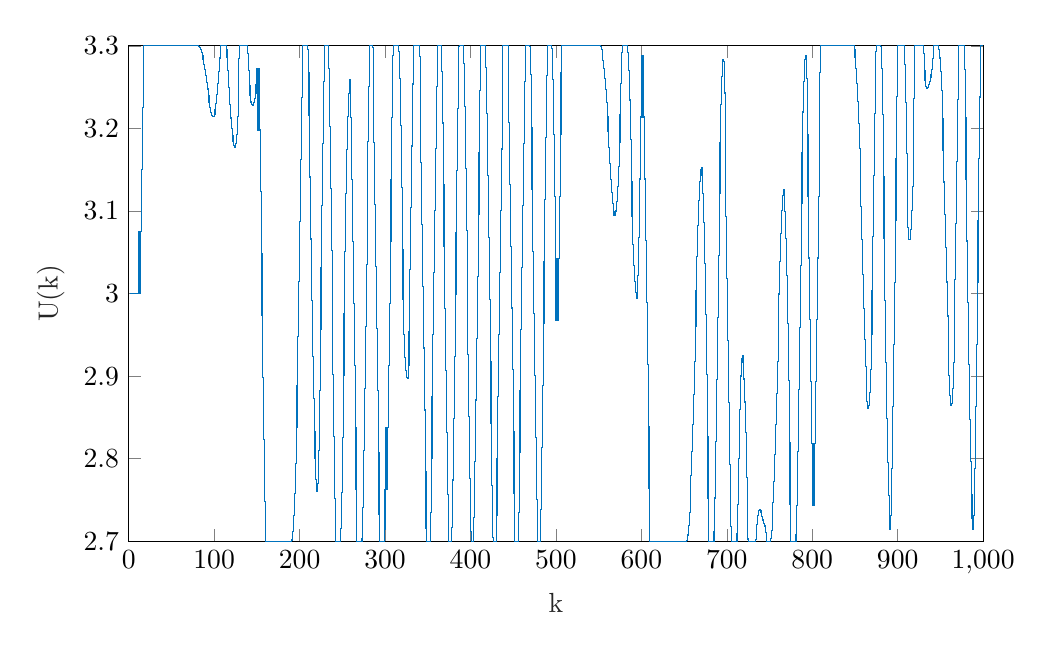
\begin{tikzpicture}

\begin{axis}[%
width=4.272in,
height=2.477in,
at={(0.717in,0.437in)},
scale only axis,
xmin=0,
xmax=1000,
xlabel style={font=\color{white!15!black}},
xlabel={k},
ymin=2.7,
ymax=3.3,
ylabel style={font=\color{white!15!black}},
ylabel={U(k)},
axis background/.style={fill=white}
]
\addplot[const plot, color=mycolor1, forget plot] table[row sep=crcr] {%
1	3\\
2	3\\
3	3\\
4	3\\
5	3\\
6	3\\
7	3\\
8	3\\
9	3\\
10	3\\
11	3\\
12	3.075\\
13	3\\
14	3.075\\
15	3.15\\
16	3.225\\
17	3.3\\
18	3.3\\
19	3.3\\
20	3.3\\
21	3.3\\
22	3.3\\
23	3.3\\
24	3.3\\
25	3.3\\
26	3.3\\
27	3.3\\
28	3.3\\
29	3.3\\
30	3.3\\
31	3.3\\
32	3.3\\
33	3.3\\
34	3.3\\
35	3.3\\
36	3.3\\
37	3.3\\
38	3.3\\
39	3.3\\
40	3.3\\
41	3.3\\
42	3.3\\
43	3.3\\
44	3.3\\
45	3.3\\
46	3.3\\
47	3.3\\
48	3.3\\
49	3.3\\
50	3.3\\
51	3.3\\
52	3.3\\
53	3.3\\
54	3.3\\
55	3.3\\
56	3.3\\
57	3.3\\
58	3.3\\
59	3.3\\
60	3.3\\
61	3.3\\
62	3.3\\
63	3.3\\
64	3.3\\
65	3.3\\
66	3.3\\
67	3.3\\
68	3.3\\
69	3.3\\
70	3.3\\
71	3.3\\
72	3.3\\
73	3.3\\
74	3.3\\
75	3.3\\
76	3.3\\
77	3.3\\
78	3.3\\
79	3.3\\
80	3.3\\
81	3.3\\
82	3.29960688967949\\
83	3.29817127645671\\
84	3.29575541273248\\
85	3.29241820651487\\
86	3.28821536111669\\
87	3.28319951377967\\
88	3.2774203725041\\
89	3.2709248504854\\
90	3.2637571976671\\
91	3.25595912901356\\
92	3.24768725885909\\
93	3.23938628121859\\
94	3.2316144120574\\
95	3.22483270422986\\
96	3.21942304526205\\
97	3.21570355060128\\
98	3.21394167140295\\
99	3.21436530092808\\
100	3.21717213217181\\
101	3.22253749109725\\
102	3.230585837643\\
103	3.2412806530834\\
104	3.25433048376625\\
105	3.26921718691069\\
106	3.28527254042179\\
107	3.3\\
108	3.3\\
109	3.3\\
110	3.3\\
111	3.3\\
112	3.3\\
113	3.3\\
114	3.29572914972939\\
115	3.28571450719575\\
116	3.26989641769384\\
117	3.24908696887181\\
118	3.22862771135804\\
119	3.21252096308746\\
120	3.2000893423487\\
121	3.1907366020886\\
122	3.18393891058865\\
123	3.17923701581878\\
124	3.17750368911651\\
125	3.18115175357714\\
126	3.19274467864678\\
127	3.21434153628636\\
128	3.24598622639231\\
129	3.28509842795535\\
130	3.3\\
131	3.3\\
132	3.3\\
133	3.3\\
134	3.3\\
135	3.3\\
136	3.3\\
137	3.3\\
138	3.3\\
139	3.29024204649646\\
140	3.27001095765524\\
141	3.25180796535865\\
142	3.23940939616621\\
143	3.23188981532894\\
144	3.2284355422411\\
145	3.22833259198096\\
146	3.23095584183106\\
147	3.23575930285311\\
148	3.24226738804828\\
149	3.25297899012864\\
150	3.27305934790897\\
151	3.19805934790897\\
152	3.27305934790897\\
153	3.19805934790897\\
154	3.12305934790897\\
155	3.04805934790897\\
156	2.97305934790897\\
157	2.89805934790897\\
158	2.82305934790897\\
159	2.74805934790897\\
160	2.7\\
161	2.7\\
162	2.7\\
163	2.7\\
164	2.7\\
165	2.7\\
166	2.7\\
167	2.7\\
168	2.7\\
169	2.7\\
170	2.7\\
171	2.7\\
172	2.7\\
173	2.7\\
174	2.7\\
175	2.7\\
176	2.7\\
177	2.7\\
178	2.7\\
179	2.7\\
180	2.7\\
181	2.7\\
182	2.7\\
183	2.7\\
184	2.7\\
185	2.7\\
186	2.7\\
187	2.7\\
188	2.7\\
189	2.7\\
190	2.7\\
191	2.70147723464141\\
192	2.71176763298304\\
193	2.73071318638751\\
194	2.75812490555953\\
195	2.79378881658902\\
196	2.83747119050711\\
197	2.88892309130814\\
198	2.94788431862728\\
199	3.01408681336634\\
200	3.08725758744632\\
201	3.16225758744632\\
202	3.23725758744632\\
203	3.3\\
204	3.3\\
205	3.3\\
206	3.3\\
207	3.3\\
208	3.3\\
209	3.29516704570335\\
210	3.26713969527367\\
211	3.21536893814701\\
212	3.14106903639367\\
213	3.06606903639367\\
214	2.99106903639367\\
215	2.92410345636304\\
216	2.87253351998596\\
217	2.83237746050336\\
218	2.80019564530833\\
219	2.77447105167493\\
220	2.76077846100121\\
221	2.7694325349364\\
222	2.80941961252196\\
223	2.8820134292749\\
224	2.9570134292749\\
225	3.0320134292749\\
226	3.1070134292749\\
227	3.1820134292749\\
228	3.2570134292749\\
229	3.3\\
230	3.3\\
231	3.3\\
232	3.3\\
233	3.3\\
234	3.2723732879358\\
235	3.20219283239161\\
236	3.12719283239161\\
237	3.05219283239161\\
238	2.97719283239161\\
239	2.90219283239161\\
240	2.82719283239161\\
241	2.75219283239161\\
242	2.7\\
243	2.7\\
244	2.7\\
245	2.7\\
246	2.7\\
247	2.7\\
248	2.71579632030559\\
249	2.75887890480879\\
250	2.8260330185042\\
251	2.9010330185042\\
252	2.9760330185042\\
253	3.0510330185042\\
254	3.12163481254492\\
255	3.17476273843773\\
256	3.21404597378946\\
257	3.24264159428616\\
258	3.25857346312169\\
259	3.25218366995886\\
260	3.2126365698168\\
261	3.1376365698168\\
262	3.0626365698168\\
263	2.9876365698168\\
264	2.9126365698168\\
265	2.8376365698168\\
266	2.7626365698168\\
267	2.7\\
268	2.7\\
269	2.7\\
270	2.7\\
271	2.7\\
272	2.7\\
273	2.70277840481037\\
274	2.74081445262293\\
275	2.8096383818149\\
276	2.8846383818149\\
277	2.9596383818149\\
278	3.0346383818149\\
279	3.1096383818149\\
280	3.1846383818149\\
281	3.25096984094573\\
282	3.3\\
283	3.3\\
284	3.3\\
285	3.29822927604903\\
286	3.25788915596759\\
287	3.18288915596759\\
288	3.10788915596759\\
289	3.03288915596759\\
290	2.95788915596759\\
291	2.88288915596759\\
292	2.80788915596759\\
293	2.73288915596759\\
294	2.7\\
295	2.7\\
296	2.7\\
297	2.7\\
298	2.7\\
299	2.7148407513352\\
300	2.76277418990821\\
301	2.83777418990821\\
302	2.76277418990821\\
303	2.83777418990821\\
304	2.91277418990821\\
305	2.98777418990821\\
306	3.06277418990821\\
307	3.13777418990821\\
308	3.21277418990821\\
309	3.28777418990821\\
310	3.3\\
311	3.3\\
312	3.3\\
313	3.3\\
314	3.3\\
315	3.3\\
316	3.29337297267092\\
317	3.26028326003254\\
318	3.20354106439256\\
319	3.12854106439256\\
320	3.05354106439256\\
321	2.99285695333478\\
322	2.95056959436638\\
323	2.92283784468324\\
324	2.90632086214506\\
325	2.89812219021248\\
326	2.89771723622663\\
327	2.91247817310165\\
328	2.95369498316833\\
329	3.02869498316833\\
330	3.10369498316833\\
331	3.17869498316833\\
332	3.25369498316833\\
333	3.3\\
334	3.3\\
335	3.3\\
336	3.3\\
337	3.3\\
338	3.3\\
339	3.3\\
340	3.28655824617185\\
341	3.23395347984281\\
342	3.15895347984281\\
343	3.08395347984281\\
344	3.00895347984281\\
345	2.93395347984281\\
346	2.85895347984281\\
347	2.78415046502553\\
348	2.71564475781247\\
349	2.7\\
350	2.7\\
351	2.7\\
352	2.7\\
353	2.73468571820584\\
354	2.80075221736396\\
355	2.87575221736396\\
356	2.95075221736396\\
357	3.02575221736396\\
358	3.10075221736396\\
359	3.17575221736396\\
360	3.25075221736396\\
361	3.3\\
362	3.3\\
363	3.3\\
364	3.3\\
365	3.3\\
366	3.26942602133464\\
367	3.20648846271432\\
368	3.13148846271432\\
369	3.05648846271432\\
370	2.98148846271432\\
371	2.90648846271433\\
372	2.83148846271432\\
373	2.75648846271432\\
374	2.7\\
375	2.7\\
376	2.7\\
377	2.7\\
378	2.71704056968883\\
379	2.77411723026836\\
380	2.84911723026836\\
381	2.92411723026836\\
382	2.99911723026836\\
383	3.07411723026837\\
384	3.14911723026836\\
385	3.22411723026836\\
386	3.29911723026837\\
387	3.3\\
388	3.3\\
389	3.3\\
390	3.3\\
391	3.3\\
392	3.27839087299347\\
393	3.22647913379567\\
394	3.15147913379567\\
395	3.07647913379567\\
396	3.00147913379567\\
397	2.92647913379567\\
398	2.85147913379567\\
399	2.77647913379567\\
400	2.7120851797893\\
401	2.7\\
402	2.7\\
403	2.7\\
404	2.72844743912458\\
405	2.79602375367187\\
406	2.87102375367187\\
407	2.94602375367187\\
408	3.02102375367187\\
409	3.09602375367187\\
410	3.17102375367187\\
411	3.24602375367187\\
412	3.3\\
413	3.3\\
414	3.3\\
415	3.3\\
416	3.3\\
417	3.3\\
418	3.27410647374472\\
419	3.21774356706703\\
420	3.14274356706703\\
421	3.06774356706703\\
422	2.99274356706703\\
423	2.91774356706703\\
424	2.84274356706703\\
425	2.76774356706703\\
426	2.70500958120977\\
427	2.7\\
428	2.7\\
429	2.7\\
430	2.73099087142221\\
431	2.80003930324114\\
432	2.87503930324114\\
433	2.95003930324114\\
434	3.02503930324114\\
435	3.10003930324114\\
436	3.17503930324114\\
437	3.25003930324114\\
438	3.3\\
439	3.3\\
440	3.3\\
441	3.3\\
442	3.3\\
443	3.3\\
444	3.2687377298274\\
445	3.207454038266\\
446	3.132454038266\\
447	3.057454038266\\
448	2.982454038266\\
449	2.907454038266\\
450	2.832454038266\\
451	2.757454038266\\
452	2.7\\
453	2.7\\
454	2.7\\
455	2.7\\
456	2.73472766040337\\
457	2.80694677522055\\
458	2.88194677522055\\
459	2.95694677522055\\
460	3.03194677522055\\
461	3.10694677522055\\
462	3.18194677522055\\
463	3.25694677522055\\
464	3.3\\
465	3.3\\
466	3.3\\
467	3.3\\
468	3.3\\
469	3.29939889284135\\
470	3.26474252459835\\
471	3.20058906113808\\
472	3.12558906113808\\
473	3.05058906113808\\
474	2.97558906113808\\
475	2.90058906113808\\
476	2.82558906113808\\
477	2.75058906113808\\
478	2.7\\
479	2.7\\
480	2.7\\
481	2.7\\
482	2.73878157380437\\
483	2.81378157380437\\
484	2.88878157380437\\
485	2.96378157380437\\
486	3.03878157380437\\
487	3.11378157380437\\
488	3.18878157380437\\
489	3.26378157380437\\
490	3.3\\
491	3.3\\
492	3.3\\
493	3.3\\
494	3.3\\
495	3.29627913229756\\
496	3.25896634835273\\
497	3.1925287456284\\
498	3.1175287456284\\
499	3.0425287456284\\
500	2.9675287456284\\
501	3.0425287456284\\
502	2.9675287456284\\
503	3.0425287456284\\
504	3.1175287456284\\
505	3.1925287456284\\
506	3.2675287456284\\
507	3.3\\
508	3.3\\
509	3.3\\
510	3.3\\
511	3.3\\
512	3.3\\
513	3.3\\
514	3.3\\
515	3.3\\
516	3.3\\
517	3.3\\
518	3.3\\
519	3.3\\
520	3.3\\
521	3.3\\
522	3.3\\
523	3.3\\
524	3.3\\
525	3.3\\
526	3.3\\
527	3.3\\
528	3.3\\
529	3.3\\
530	3.3\\
531	3.3\\
532	3.3\\
533	3.3\\
534	3.3\\
535	3.3\\
536	3.3\\
537	3.3\\
538	3.3\\
539	3.3\\
540	3.3\\
541	3.3\\
542	3.3\\
543	3.3\\
544	3.3\\
545	3.3\\
546	3.3\\
547	3.3\\
548	3.3\\
549	3.3\\
550	3.3\\
551	3.3\\
552	3.29894453967181\\
553	3.29554155949028\\
554	3.28990160219775\\
555	3.28213244833643\\
556	3.27233885321272\\
557	3.26062234386232\\
558	3.24708106804495\\
559	3.23180968819684\\
560	3.21489931407361\\
561	3.19643746853702\\
562	3.17682304584946\\
563	3.15709624470148\\
564	3.13851031991325\\
565	3.12211766988767\\
566	3.10880559666185\\
567	3.09932721493915\\
568	3.09432804998037\\
569	3.09436881275852\\
570	3.0999447935108\\
571	3.11150227147876\\
572	3.12935830916555\\
573	3.15344240949369\\
574	3.18310315947256\\
575	3.21717949312761\\
576	3.25416418741236\\
577	3.29232295139274\\
578	3.3\\
579	3.3\\
580	3.3\\
581	3.3\\
582	3.3\\
583	3.3\\
584	3.29148795470058\\
585	3.26969102570955\\
586	3.23439851094328\\
587	3.18620941262121\\
588	3.13541354610641\\
589	3.09299273231174\\
590	3.05975314362913\\
591	3.0342150859982\\
592	3.01507818829214\\
593	3.00120201929974\\
594	2.99412879028123\\
595	2.99904316883138\\
596	3.02193091003428\\
597	3.06800078547562\\
598	3.13871781932088\\
599	3.21371781932088\\
600	3.28871781932089\\
601	3.21371781932088\\
602	3.28871781932089\\
603	3.21371781932088\\
604	3.13871781932088\\
605	3.06371781932088\\
606	2.98871781932088\\
607	2.91371781932089\\
608	2.83871781932088\\
609	2.76371781932088\\
610	2.7\\
611	2.7\\
612	2.7\\
613	2.7\\
614	2.7\\
615	2.7\\
616	2.7\\
617	2.7\\
618	2.7\\
619	2.7\\
620	2.7\\
621	2.7\\
622	2.7\\
623	2.7\\
624	2.7\\
625	2.7\\
626	2.7\\
627	2.7\\
628	2.7\\
629	2.7\\
630	2.7\\
631	2.7\\
632	2.7\\
633	2.7\\
634	2.7\\
635	2.7\\
636	2.7\\
637	2.7\\
638	2.7\\
639	2.7\\
640	2.7\\
641	2.7\\
642	2.7\\
643	2.7\\
644	2.7\\
645	2.7\\
646	2.7\\
647	2.7\\
648	2.7\\
649	2.7\\
650	2.7\\
651	2.7\\
652	2.7\\
653	2.70120705805128\\
654	2.70756189807642\\
655	2.71883429678429\\
656	2.73479812800667\\
657	2.75523217690026\\
658	2.77992079692193\\
659	2.80865442966426\\
660	2.84123000541235\\
661	2.87745124028702\\
662	2.91712884405002\\
663	2.95972044787705\\
664	3.00321834917897\\
665	3.0448001756255\\
666	3.08209099732749\\
667	3.1130850427763\\
668	3.13607783766497\\
669	3.14960763531297\\
670	3.15240511111252\\
671	3.14335038925055\\
672	3.12143655835466\\
673	3.08584640379987\\
674	3.03645460828551\\
675	2.9743903304998\\
676	2.90197687098003\\
677	2.82697687098003\\
678	2.75197687098003\\
679	2.7\\
680	2.7\\
681	2.7\\
682	2.7\\
683	2.7\\
684	2.7\\
685	2.71183044346158\\
686	2.75234977840967\\
687	2.82104919152645\\
688	2.89604919152645\\
689	2.97104919152645\\
690	3.04604919152645\\
691	3.12104919152645\\
692	3.1824727676357\\
693	3.22895616758794\\
694	3.26311593483973\\
695	3.28371285675021\\
696	3.28128058562129\\
697	3.24286554835967\\
698	3.16786554835967\\
699	3.09286554835967\\
700	3.01786554835967\\
701	2.94286554835967\\
702	2.86786554835967\\
703	2.79286554835967\\
704	2.71786554835967\\
705	2.7\\
706	2.7\\
707	2.7\\
708	2.7\\
709	2.7\\
710	2.7\\
711	2.7\\
712	2.70978963629078\\
713	2.74424534005188\\
714	2.80053227056236\\
715	2.85946445688434\\
716	2.90014159369498\\
717	2.92083660240976\\
718	2.92511005376372\\
719	2.91607750828044\\
720	2.89645833076236\\
721	2.86861949859498\\
722	2.83169353124213\\
723	2.77769058204749\\
724	2.70269058204749\\
725	2.7\\
726	2.7\\
727	2.7\\
728	2.7\\
729	2.7\\
730	2.7\\
731	2.7\\
732	2.7\\
733	2.7\\
734	2.7018540165753\\
735	2.71982612040244\\
736	2.73134914142033\\
737	2.73721461197819\\
738	2.73886486461053\\
739	2.73754636887\\
740	2.73433201475295\\
741	2.7301410642449\\
742	2.72575700357151\\
743	2.72184350624163\\
744	2.71840543187559\\
745	2.71064272251494\\
746	2.7\\
747	2.7\\
748	2.7\\
749	2.7\\
750	2.7\\
751	2.70350382449205\\
752	2.71290102566989\\
753	2.72766520512821\\
754	2.7471478029978\\
755	2.77221280258811\\
756	2.80454258073494\\
757	2.84118060148726\\
758	2.87891776061295\\
759	2.91794850341493\\
760	2.95842895446127\\
761	2.99943624823676\\
762	3.03844458213756\\
763	3.07269829352415\\
764	3.10007904848175\\
765	3.11858723418108\\
766	3.12563563189682\\
767	3.11925378988416\\
768	3.09937103059158\\
769	3.06661751506282\\
770	3.02128149635603\\
771	2.96368278052773\\
772	2.89495020965423\\
773	2.81995020965423\\
774	2.74495020965423\\
775	2.7\\
776	2.7\\
777	2.7\\
778	2.7\\
779	2.7\\
780	2.7\\
781	2.70773489643216\\
782	2.74377562270011\\
783	2.80899872631388\\
784	2.88399872631388\\
785	2.95899872631388\\
786	3.03399872631388\\
787	3.10899872631388\\
788	3.1712960063952\\
789	3.21986736851672\\
790	3.25712839028565\\
791	3.28288562642989\\
792	3.28863875010106\\
793	3.26083088466387\\
794	3.19299438407716\\
795	3.11799438407716\\
796	3.04299438407716\\
797	2.96799438407716\\
798	2.89299438407716\\
799	2.81799438407716\\
800	2.74299438407716\\
801	2.81799438407716\\
802	2.74299438407716\\
803	2.81799438407716\\
804	2.89299438407716\\
805	2.96799438407716\\
806	3.04299438407716\\
807	3.11799438407716\\
808	3.19299438407716\\
809	3.26799438407716\\
810	3.3\\
811	3.3\\
812	3.3\\
813	3.3\\
814	3.3\\
815	3.3\\
816	3.3\\
817	3.3\\
818	3.3\\
819	3.3\\
820	3.3\\
821	3.3\\
822	3.3\\
823	3.3\\
824	3.3\\
825	3.3\\
826	3.3\\
827	3.3\\
828	3.3\\
829	3.3\\
830	3.3\\
831	3.3\\
832	3.3\\
833	3.3\\
834	3.3\\
835	3.3\\
836	3.3\\
837	3.3\\
838	3.3\\
839	3.3\\
840	3.3\\
841	3.3\\
842	3.3\\
843	3.3\\
844	3.3\\
845	3.3\\
846	3.3\\
847	3.3\\
848	3.3\\
849	3.29541295140333\\
850	3.28616605135574\\
851	3.27243264706671\\
852	3.25438801722897\\
853	3.23220795182076\\
854	3.20606754805635\\
855	3.17614019679584\\
856	3.14259673647546\\
857	3.10560475409101\\
858	3.06532801498864\\
859	3.02329484528497\\
860	2.98217762566906\\
861	2.94431506522496\\
862	2.91170223195827\\
863	2.88605066854032\\
864	2.8688408372583\\
865	2.86136764876848\\
866	2.86477977345999\\
867	2.88011338054179\\
868	2.90832089860909\\
869	2.94988686139046\\
870	3.00416921024664\\
871	3.06932010302979\\
872	3.1426267127859\\
873	3.2176267127859\\
874	3.2926267127859\\
875	3.3\\
876	3.3\\
877	3.3\\
878	3.3\\
879	3.3\\
880	3.29933019929396\\
881	3.27208102246009\\
882	3.21680469329493\\
883	3.14180469329493\\
884	3.06680469329493\\
885	2.99180469329493\\
886	2.91680469329493\\
887	2.84818694409016\\
888	2.79523805497731\\
889	2.75527027996251\\
890	2.72612792866643\\
891	2.71384758553663\\
892	2.7314837887125\\
893	2.7885023911345\\
894	2.8635023911345\\
895	2.9385023911345\\
896	3.0135023911345\\
897	3.0885023911345\\
898	3.1635023911345\\
899	3.2385023911345\\
900	3.3\\
901	3.3\\
902	3.3\\
903	3.3\\
904	3.3\\
905	3.3\\
906	3.3\\
907	3.3\\
908	3.27750126536057\\
909	3.23171632899537\\
910	3.16920121831105\\
911	3.11349389146534\\
912	3.08013596070663\\
913	3.06528215509634\\
914	3.06556287165494\\
915	3.07803225012136\\
916	3.10012155820866\\
917	3.12959736521866\\
918	3.17123797201646\\
919	3.23584843824045\\
920	3.3\\
921	3.3\\
922	3.3\\
923	3.3\\
924	3.3\\
925	3.3\\
926	3.3\\
927	3.3\\
928	3.3\\
929	3.3\\
930	3.29077494325808\\
931	3.27040342373973\\
932	3.2577016874232\\
933	3.25096026391623\\
934	3.24869565000019\\
935	3.24962489212234\\
936	3.2526428123752\\
937	3.25680161529795\\
938	3.26129263817939\\
939	3.26543003048947\\
940	3.2713890560364\\
941	3.28428001221313\\
942	3.3\\
943	3.3\\
944	3.3\\
945	3.3\\
946	3.3\\
947	3.3\\
948	3.29539623798284\\
949	3.28517461663894\\
950	3.26934057323485\\
951	3.24575569145582\\
952	3.21231709543726\\
953	3.17384394573857\\
954	3.13505984335751\\
955	3.09565526873873\\
956	3.05537249412054\\
957	3.01399923116038\\
958	2.97273679678414\\
959	2.93425493923369\\
960	2.90120519331087\\
961	2.87659713464477\\
962	2.8643726944093\\
963	2.86724457563175\\
964	2.88495860989809\\
965	2.91621512189692\\
966	2.96020956534409\\
967	3.01654185165116\\
968	3.08473103341843\\
969	3.15973103341843\\
970	3.23473103341843\\
971	3.3\\
972	3.3\\
973	3.3\\
974	3.3\\
975	3.3\\
976	3.3\\
977	3.3\\
978	3.27175153185587\\
979	3.21358485153747\\
980	3.13858485153747\\
981	3.06358485153747\\
982	2.98858485153747\\
983	2.91358485153747\\
984	2.8476602146334\\
985	2.79626780049677\\
986	2.75688551216049\\
987	2.72730405183376\\
988	2.7140224747166\\
989	2.73122625211251\\
990	2.7880105747135\\
991	2.8630105747135\\
992	2.9380105747135\\
993	3.0130105747135\\
994	3.0880105747135\\
995	3.1630105747135\\
996	3.2380105747135\\
997	3.3\\
998	3.3\\
999	3.3\\
1000	3.3\\
};
\end{axis}
\end{tikzpicture}%
\caption{Sterowanie PID dla parametrów $K=1,4$, $T_i=1,35$,  $T_d=19,55$}
\end{figure}

\begin{figure}[H]
\centering
% This file was created by matlab2tikz.
%
%The latest updates can be retrieved from
%  http://www.mathworks.com/matlabcentral/fileexchange/22022-matlab2tikz-matlab2tikz
%where you can also make suggestions and rate matlab2tikz.
%
\definecolor{mycolor1}{rgb}{0.00000,0.44700,0.74100}%
\definecolor{mycolor2}{rgb}{0.85000,0.32500,0.09800}%
%
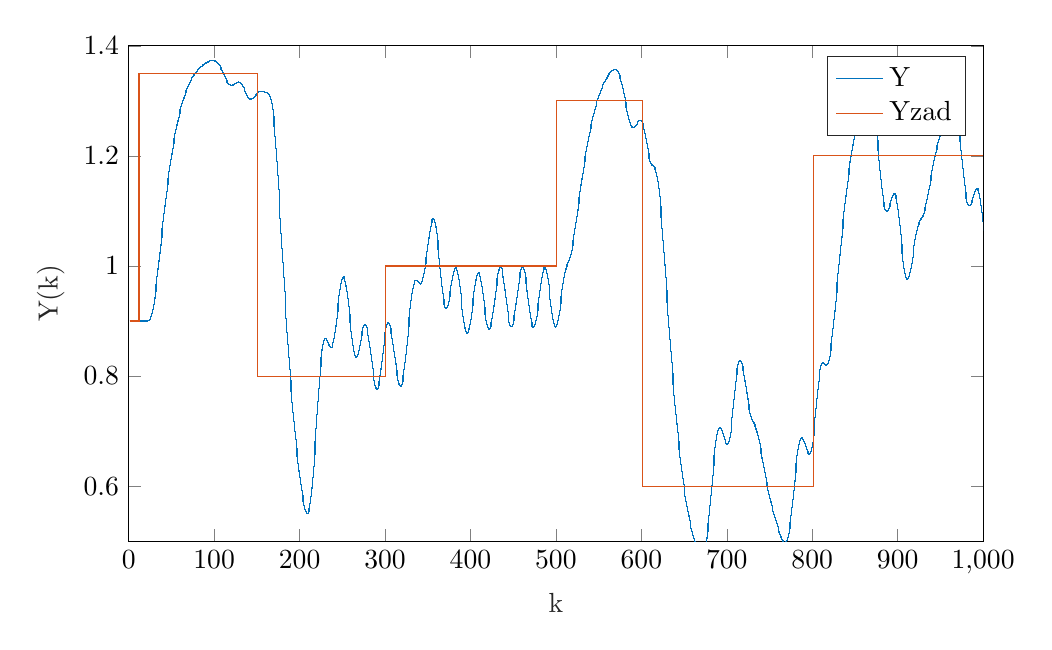
\begin{tikzpicture}

\begin{axis}[%
width=4.272in,
height=2.477in,
at={(0.717in,0.437in)},
scale only axis,
xmin=0,
xmax=1000,
xlabel style={font=\color{white!15!black}},
xlabel={k},
ymin=0.5,
ymax=1.4,
ylabel style={font=\color{white!15!black}},
ylabel={Y(k)},
axis background/.style={fill=white},
legend style={legend cell align=left, align=left, draw=white!15!black}
]
\addplot[const plot, color=mycolor1] table[row sep=crcr] {%
1	0.9\\
2	0.9\\
3	0.9\\
4	0.9\\
5	0.9\\
6	0.9\\
7	0.9\\
8	0.9\\
9	0.9\\
10	0.9\\
11	0.9\\
12	0.9\\
13	0.9\\
14	0.9\\
15	0.9\\
16	0.9\\
17	0.9\\
18	0.9\\
19	0.9\\
20	0.9\\
21	0.9\\
22	0.9003968325\\
23	0.90110505465075\\
24	0.902093616629444\\
25	0.904084951636002\\
26	0.907683459193576\\
27	0.913389873194666\\
28	0.921217241044141\\
29	0.930787780218191\\
30	0.941770919296453\\
31	0.953878119503626\\
32	0.966858227313968\\
33	0.980493305812802\\
34	0.994594897526365\\
35	1.00900067597601\\
36	1.02357144732894\\
37	1.03818846724494\\
38	1.05275104139355\\
39	1.06717438117128\\
40	1.08138768891386\\
41	1.09533244940115\\
42	1.108960906717\\
43	1.12223470757455\\
44	1.13512369407114\\
45	1.14760483051195\\
46	1.15966125045738\\
47	1.17128141151831\\
48	1.18245834666161\\
49	1.19318900190664\\
50	1.2034736513041\\
51	1.21331538100131\\
52	1.2227196350219\\
53	1.23169381613216\\
54	1.24024693583765\\
55	1.24838930815927\\
56	1.25613228238498\\
57	1.26348801048556\\
58	1.27046924532749\\
59	1.27708916621625\\
60	1.28336122866391\\
61	1.28929903559995\\
62	1.29491622753654\\
63	1.30022638946269\\
64	1.30524297247869\\
65	1.30997922839486\\
66	1.31444815571025\\
67	1.31866245555886\\
68	1.32263449636529\\
69	1.32637628609039\\
70	1.32989945107198\\
71	1.33321522057705\\
72	1.3363344162819\\
73	1.33926744598615\\
74	1.34202430094677\\
75	1.34461455628992\\
76	1.3470473740223\\
77	1.34933150822129\\
78	1.35147531203391\\
79	1.35348674616047\\
80	1.35537338853904\\
81	1.35714244498348\\
82	1.35880076055936\\
83	1.36035483151118\\
84	1.36181081757928\\
85	1.36317455456734\\
86	1.36445156704152\\
87	1.36564708105938\\
88	1.36676603684269\\
89	1.36781310132169\\
90	1.36879268049023\\
91	1.36970893152209\\
92	1.37056369462176\\
93	1.37135143640827\\
94	1.37205750489042\\
95	1.37266025521426\\
96	1.37313285804773\\
97	1.37344482949402\\
98	1.3735633171834\\
99	1.37345417337891\\
100	1.37308284250311\\
101	1.3724150874145\\
102	1.37141819669726\\
103	1.37006409478304\\
104	1.36833398386579\\
105	1.36622226313627\\
106	1.36373885303598\\
107	1.3609103275734\\
108	1.35778017798024\\
109	1.35440846457425\\
110	1.35087105865836\\
111	1.34725863091188\\
112	1.34367532031541\\
113	1.34023641628249\\
114	1.33706417324462\\
115	1.33428175238138\\
116	1.33200616529444\\
117	1.33033192252879\\
118	1.32925051596625\\
119	1.32867727341544\\
120	1.32853735228886\\
121	1.3287646999217\\
122	1.32930111826576\\
123	1.33009542281877\\
124	1.33108008911642\\
125	1.3321450480117\\
126	1.33313727820844\\
127	1.33387242007725\\
128	1.33417312304507\\
129	1.33391699925013\\
130	1.33304535538812\\
131	1.33154718366126\\
132	1.32944611002816\\
133	1.32678984129904\\
134	1.32364845951129\\
135	1.32012764956961\\
136	1.31638815762936\\
137	1.31265997566391\\
138	1.30924070526468\\
139	1.30646977420847\\
140	1.30453927990026\\
141	1.30340628557131\\
142	1.30295482863853\\
143	1.30308250089857\\
144	1.30369900978869\\
145	1.30472488439263\\
146	1.30609031211015\\
147	1.30773409324782\\
148	1.30960270200292\\
149	1.31159781310476\\
150	1.31353124752258\\
151	1.31520262628755\\
152	1.31648506489343\\
153	1.31732862761217\\
154	1.31773982309575\\
155	1.31776499329167\\
156	1.31747698281417\\
157	1.31696456158061\\
158	1.31632414815446\\
159	1.31566885338501\\
160	1.31516500979491\\
161	1.31449607632197\\
162	1.31371343302732\\
163	1.31281806449549\\
164	1.31106104463425\\
165	1.30781467100108\\
166	1.30255775304501\\
167	1.29486249163885\\
168	1.28438278801863\\
169	1.27084383610959\\
170	1.25417541224886\\
171	1.23472724723621\\
172	1.21305327933571\\
173	1.18963610848809\\
174	1.1648949294421\\
175	1.13919264501029\\
176	1.11284224059512\\
177	1.08611249332229\\
178	1.05923308204585\\
179	1.03239915808653\\
180	1.00577543076717\\
181	0.979499816561736\\
182	0.953686695925049\\
183	0.92842981757281\\
184	0.903804886093526\\
185	0.879871865256793\\
186	0.856677026201692\\
187	0.834254766812913\\
188	0.812629225992097\\
189	0.791815714181749\\
190	0.771821979375336\\
191	0.752649325928511\\
192	0.734293601753279\\
193	0.716746067911899\\
194	0.699994163214376\\
195	0.684022175148048\\
196	0.668811827317021\\
197	0.654342792531058\\
198	0.640593139747328\\
199	0.627539722224302\\
200	0.615158513486347\\
201	0.603432713208305\\
202	0.592397944331922\\
203	0.582169792765051\\
204	0.572928922843505\\
205	0.56490778875359\\
206	0.558378838055793\\
207	0.553644102506015\\
208	0.551026072071361\\
209	0.550859750038763\\
210	0.553485790125525\\
211	0.559218886244527\\
212	0.568314378923628\\
213	0.580901783120207\\
214	0.596674951956446\\
215	0.615040736514964\\
216	0.635481036645496\\
217	0.657544521771329\\
218	0.680839203505885\\
219	0.705000204365535\\
220	0.729566571889155\\
221	0.753904301482308\\
222	0.777240808573632\\
223	0.798812858625823\\
224	0.817982926631092\\
225	0.834269868799955\\
226	0.847406987763883\\
227	0.857326369214658\\
228	0.864090483557596\\
229	0.867846405773905\\
230	0.868833709491585\\
231	0.86745111032582\\
232	0.86432848059569\\
233	0.860338804344058\\
234	0.856401608070486\\
235	0.853306054174515\\
236	0.851713992953739\\
237	0.852175396481653\\
238	0.855142123972007\\
239	0.860810802061028\\
240	0.868942770252105\\
241	0.879105405628047\\
242	0.890919929242386\\
243	0.904055511411159\\
244	0.918077805165622\\
245	0.932250517111628\\
246	0.945711742926951\\
247	0.957713182873563\\
248	0.967631492152522\\
249	0.974952964772594\\
250	0.979259882072809\\
251	0.980218356079364\\
252	0.977688189552021\\
253	0.971963439340018\\
254	0.963574307023995\\
255	0.952986130085843\\
256	0.940606425252086\\
257	0.926791213693531\\
258	0.911934278463504\\
259	0.896598636667336\\
260	0.881527266494752\\
261	0.867508612710653\\
262	0.855241822517237\\
263	0.845306812946982\\
264	0.838155709107306\\
265	0.834038504692047\\
266	0.832986473513785\\
267	0.834880623477667\\
268	0.839481013757128\\
269	0.846385989017177\\
270	0.854954081961934\\
271	0.864278810562834\\
272	0.873411523847959\\
273	0.881551366318569\\
274	0.888027569023697\\
275	0.892283644109796\\
276	0.893863289913455\\
277	0.89246324867111\\
278	0.888239459009213\\
279	0.881655222312419\\
280	0.873117366762481\\
281	0.862982368747728\\
282	0.851561850766269\\
283	0.839142217785733\\
284	0.826172472172082\\
285	0.813375068945223\\
286	0.801546456969581\\
287	0.791384733613487\\
288	0.783469472114701\\
289	0.778276324289861\\
290	0.77619003222242\\
291	0.777470145350499\\
292	0.782179654378267\\
293	0.790003884473224\\
294	0.800411536157881\\
295	0.812927492748351\\
296	0.826923616119073\\
297	0.841482983124134\\
298	0.855653320173195\\
299	0.868631969737345\\
300	0.879747911675792\\
301	0.888445719788301\\
302	0.89427125727906\\
303	0.896858934019187\\
304	0.896143178550379\\
305	0.89247440095878\\
306	0.886332323338946\\
307	0.878138379842008\\
308	0.868262024984357\\
309	0.857104923891704\\
310	0.845264229168262\\
311	0.833557989556087\\
312	0.822018759174006\\
313	0.810716178670415\\
314	0.800458094654311\\
315	0.791920856656079\\
316	0.785665304789147\\
317	0.782151026578178\\
318	0.781749059123875\\
319	0.784753195506041\\
320	0.791057894192873\\
321	0.800174036409754\\
322	0.811608910821106\\
323	0.824931090106648\\
324	0.839763723715891\\
325	0.855778517600725\\
326	0.872655269053406\\
327	0.889944557098732\\
328	0.907006210308025\\
329	0.923085478629688\\
330	0.937459160711599\\
331	0.94960245236246\\
332	0.95925487044782\\
333	0.966381175882662\\
334	0.971099904220388\\
335	0.973626808501042\\
336	0.974241191106598\\
337	0.9733106801145\\
338	0.971371851039053\\
339	0.969195945974342\\
340	0.967605591453123\\
341	0.967292570685363\\
342	0.968833611439064\\
343	0.972552643022897\\
344	0.978321037311681\\
345	0.985785250044053\\
346	0.994635506308991\\
347	1.00460102074062\\
348	1.01544570665982\\
349	1.02696432608188\\
350	1.03890791545263\\
351	1.05078878908115\\
352	1.06188057429148\\
353	1.0714621253189\\
354	1.07893337891809\\
355	1.08380048751867\\
356	1.08566256952789\\
357	1.08420095399756\\
358	1.07920178154575\\
359	1.07081807368814\\
360	1.05954812302293\\
361	1.04590998174815\\
362	1.03035681941713\\
363	1.01346757262558\\
364	0.996079861641148\\
365	0.979109356940515\\
366	0.963372283882921\\
367	0.949550867047085\\
368	0.938209667114493\\
369	0.929810146753165\\
370	0.924723645899651\\
371	0.923106671588162\\
372	0.924679927109635\\
373	0.928940453119538\\
374	0.935445798960946\\
375	0.943807505756506\\
376	0.953523480836795\\
377	0.963836330864832\\
378	0.973876114727723\\
379	0.98284869403126\\
380	0.99008945487232\\
381	0.995047549833974\\
382	0.997271846486835\\
383	0.996398408671033\\
384	0.99223730025893\\
385	0.98504047437484\\
386	0.975323009053843\\
387	0.963536534866996\\
388	0.950166310477148\\
389	0.935929850423817\\
390	0.921734499909566\\
391	0.908436830253897\\
392	0.896755327349955\\
393	0.887287127553184\\
394	0.880522944512226\\
395	0.876860370909769\\
396	0.876615721058621\\
397	0.879642402321179\\
398	0.885420039953815\\
399	0.893486634316506\\
400	0.903436915390534\\
401	0.914916171780126\\
402	0.927500373506229\\
403	0.940555482635797\\
404	0.95326863396301\\
405	0.964839223299838\\
406	0.97459765220204\\
407	0.981989373011791\\
408	0.986560662616193\\
409	0.987945948883005\\
410	0.985912648645732\\
411	0.980615826915307\\
412	0.972533132849975\\
413	0.962146712967497\\
414	0.950029484239021\\
415	0.937026288160447\\
416	0.92409215745921\\
417	0.912071272471\\
418	0.901671542897078\\
419	0.89348113099521\\
420	0.887983188321235\\
421	0.885568987712558\\
422	0.886438375620933\\
423	0.89034852749349\\
424	0.896804620325778\\
425	0.905371987245393\\
426	0.915669605257557\\
427	0.927364245813193\\
428	0.940028217993009\\
429	0.953002938373037\\
430	0.965478530751221\\
431	0.976680194112626\\
432	0.985960987344831\\
433	0.992786215306112\\
434	0.996719508871874\\
435	0.997410426327404\\
436	0.994648321117447\\
437	0.988643985843986\\
438	0.979911708860874\\
439	0.968928843734942\\
440	0.956277372470846\\
441	0.942816459818517\\
442	0.929499609927491\\
443	0.917161865440447\\
444	0.906502988637188\\
445	0.89810388377211\\
446	0.8924412428519\\
447	0.889900595598966\\
448	0.890655441176752\\
449	0.89444175828924\\
450	0.900766952154797\\
451	0.909198285074335\\
452	0.919356398033328\\
453	0.930909491592744\\
454	0.943402689653326\\
455	0.956130120071509\\
456	0.968270691327746\\
457	0.979065301006519\\
458	0.987880742169601\\
459	0.994194305029224\\
460	0.997580050480969\\
461	0.997696585043464\\
462	0.994369020916027\\
463	0.987863313712417\\
464	0.978712123064005\\
465	0.967382743783163\\
466	0.954467961564959\\
467	0.940851243758351\\
468	0.927486345580964\\
469	0.915191968748418\\
470	0.904653474224663\\
471	0.896439097057943\\
472	0.891014405630464\\
473	0.888755184020648\\
474	0.8897898650776\\
475	0.893818322774756\\
476	0.900352236491943\\
477	0.908962696226276\\
478	0.919273768675807\\
479	0.930953537794273\\
480	0.943529411654619\\
481	0.95626962134941\\
482	0.968349434541793\\
483	0.979021499186959\\
484	0.987662938721725\\
485	0.993760107012623\\
486	0.996894999589771\\
487	0.996733152238449\\
488	0.993142035319266\\
489	0.986421346938054\\
490	0.977097618291335\\
491	0.96563269096347\\
492	0.95263595287075\\
493	0.939018112370197\\
494	0.925734356463024\\
495	0.913590157617361\\
496	0.903259249639816\\
497	0.895299669402321\\
498	0.890168060582558\\
499	0.888232416392935\\
500	0.889578223735752\\
501	0.893871093212195\\
502	0.900628229357969\\
503	0.90942565730133\\
504	0.919891848420714\\
505	0.931682307699159\\
506	0.944300934850291\\
507	0.957000807403603\\
508	0.968958860646169\\
509	0.979441101620744\\
510	0.987836384480498\\
511	0.994435006943866\\
512	0.999450729358326\\
513	1.00311760165798\\
514	1.00639262570285\\
515	1.01008745439441\\
516	1.01488565351112\\
517	1.02113309250196\\
518	1.0287283403767\\
519	1.03741455107639\\
520	1.04696757909608\\
521	1.05719236178051\\
522	1.06791967442481\\
523	1.07900322134924\\
524	1.09031702965721\\
525	1.1017531155918\\
526	1.1132193963097\\
527	1.12463782252031\\
528	1.13594270981724\\
529	1.14707924868397\\
530	1.15800217510422\\
531	1.16867458547186\\
532	1.17906688109069\\
533	1.18915582899743\\
534	1.19892372714699\\
535	1.20835766317871\\
536	1.21744885704918\\
537	1.22619207878155\\
538	1.23458513345206\\
539	1.24262840632189\\
540	1.25032446173287\\
541	1.25767769002776\\
542	1.26469399733492\\
543	1.27138053358017\\
544	1.27774545456062\\
545	1.2837977143404\\
546	1.28954688461243\\
547	1.29500299801591\\
548	1.30017641271125\\
549	1.30507769579481\\
550	1.30971752338887\\
551	1.31410659546996\\
552	1.31825556370351\\
553	1.32217497073728\\
554	1.32587519957161\\
555	1.32936643177378\\
556	1.33265861343736\\
557	1.33576142790792\\
558	1.33868427440417\\
559	1.34143625176056\\
560	1.34402614660412\\
561	1.34646242535608\\
562	1.34874764497245\\
563	1.35086723249657\\
564	1.35278634535806\\
565	1.35445434936567\\
566	1.35580867608991\\
567	1.35677812844229\\
568	1.35728569673414\\
569	1.35725094150666\\
570	1.35659199392886\\
571	1.35522721952864\\
572	1.35307825292875\\
573	1.35007749385313\\
574	1.34617871197922\\
575	1.34136587978389\\
576	1.3356585689506\\
577	1.32911474918796\\
578	1.32183166825087\\
579	1.31394535756661\\
580	1.30562919553558\\
581	1.29709186714643\\
582	1.28857448395795\\
583	1.28034524440006\\
584	1.27268973297996\\
585	1.26589700392675\\
586	1.26024341125917\\
587	1.25597608505725\\
588	1.25313969399956\\
589	1.25156972131869\\
590	1.25108055320058\\
591	1.25150833601623\\
592	1.25270866303635\\
593	1.25455449408844\\
594	1.25688924739793\\
595	1.25946452485884\\
596	1.26193089309403\\
597	1.26385784497416\\
598	1.264806522128\\
599	1.26444340181976\\
600	1.26258536692406\\
601	1.25917384444116\\
602	1.25424165469779\\
603	1.24788614087568\\
604	1.2402610314227\\
605	1.23160189325323\\
606	1.22226959123451\\
607	1.2127861281789\\
608	1.20384022032873\\
609	1.19615671317874\\
610	1.19036181276652\\
611	1.18617922421372\\
612	1.18340820640479\\
613	1.18182681367378\\
614	1.18048929735964\\
615	1.17859446616036\\
616	1.17546847964539\\
617	1.17054948512468\\
618	1.16337391140005\\
619	1.15356425113036\\
620	1.14087787515873\\
621	1.12552163587369\\
622	1.10800630708861\\
623	1.08877756623545\\
624	1.0682231994202\\
625	1.04667956380161\\
626	1.02443738067777\\
627	1.00174692561022\\
628	0.978822675526705\\
629	0.955847466957721\\
630	0.932976214324115\\
631	0.910339232450727\\
632	0.888045203189093\\
633	0.866183822147971\\
634	0.844828158015956\\
635	0.824036753781034\\
636	0.80385549627621\\
637	0.784319277879713\\
638	0.765453471847045\\
639	0.747275240626603\\
640	0.729794694589708\\
641	0.71301591687014\\
642	0.696937868440277\\
643	0.681555186134809\\
644	0.666858885054274\\
645	0.652836975626334\\
646	0.639475004561002\\
647	0.626756527996074\\
648	0.614663524281252\\
649	0.60317675308497\\
650	0.59227606681877\\
651	0.581940679753058\\
652	0.572149399638578\\
653	0.562880826144099\\
654	0.554113519967195\\
655	0.545826146066832\\
656	0.537997594099248\\
657	0.530607078808421\\
658	0.523634222825652\\
659	0.517059124066137\\
660	0.510862409670944\\
661	0.505025278227914\\
662	0.499529531812174\\
663	0.494363985878923\\
664	0.489550347194488\\
665	0.485156491300925\\
666	0.481286546727359\\
667	0.478072325656594\\
668	0.475665955413121\\
669	0.474233578441577\\
670	0.473950000734244\\
671	0.474994179998557\\
672	0.477545455286699\\
673	0.481778523523302\\
674	0.48784970211896\\
675	0.495873789781892\\
676	0.505903059560946\\
677	0.517914089525608\\
678	0.531800553720654\\
679	0.547370449250363\\
680	0.564346532649935\\
681	0.582368987851795\\
682	0.600999555844125\\
683	0.619727097220143\\
684	0.637977371736749\\
685	0.655131810035305\\
686	0.670556263556108\\
687	0.683660166924117\\
688	0.693946107656384\\
689	0.701133376137402\\
690	0.705394668030824\\
691	0.707154774451314\\
692	0.706788863873351\\
693	0.704627747750894\\
694	0.70096261648375\\
695	0.696111893311284\\
696	0.690563378739042\\
697	0.685026613832906\\
698	0.680275767968568\\
699	0.676991894567603\\
700	0.675741435674185\\
701	0.676990304183815\\
702	0.681044599537814\\
703	0.687998198551937\\
704	0.697771964268153\\
705	0.710147517351438\\
706	0.72473385924378\\
707	0.740880643543501\\
708	0.757654411864716\\
709	0.774078870558848\\
710	0.789330798927639\\
711	0.802721668064794\\
712	0.813681237559122\\
713	0.821742929460678\\
714	0.826530798529373\\
715	0.828050239627921\\
716	0.826707115543124\\
717	0.822952288589952\\
718	0.817182397754069\\
719	0.809745697706705\\
720	0.800947305351335\\
721	0.791053911860621\\
722	0.780349810572893\\
723	0.769260050173491\\
724	0.758385398016806\\
725	0.748355648514919\\
726	0.739614530917662\\
727	0.732331909959893\\
728	0.726455209211002\\
729	0.721778413713917\\
730	0.717997070936688\\
731	0.714751577314033\\
732	0.711645253079793\\
733	0.708205994034215\\
734	0.703840229808132\\
735	0.698329570204306\\
736	0.691872708259964\\
737	0.684657156153159\\
738	0.676846311047475\\
739	0.668582135119915\\
740	0.659987558708397\\
741	0.651168633976724\\
742	0.642216463858643\\
743	0.633208928655111\\
744	0.624222040284233\\
745	0.615414493110228\\
746	0.606965834706468\\
747	0.59896337494176\\
748	0.591427469642861\\
749	0.584335546189876\\
750	0.577640793530751\\
751	0.571286438400103\\
752	0.565216392585606\\
753	0.559382937553046\\
754	0.553749082933702\\
755	0.548261772488129\\
756	0.54283833383176\\
757	0.537450361111277\\
758	0.532126857864996\\
759	0.52689193397993\\
760	0.521765407457635\\
761	0.516781879761075\\
762	0.512018404014784\\
763	0.507596603264085\\
764	0.503668940763219\\
765	0.500414305945584\\
766	0.498046010992058\\
767	0.496797881258964\\
768	0.496887817678117\\
769	0.498503835553687\\
770	0.501809277513175\\
771	0.506941478191843\\
772	0.513996921970955\\
773	0.523009719259797\\
774	0.533936029519832\\
775	0.546645206665904\\
776	0.56091035296223\\
777	0.576401271817978\\
778	0.592692308192389\\
779	0.609282801748727\\
780	0.62561655739615\\
781	0.641097119371331\\
782	0.655105381699207\\
783	0.667038446497795\\
784	0.676368487670658\\
785	0.682824884050165\\
786	0.686585397931116\\
787	0.688042475870701\\
788	0.687542673423048\\
789	0.68539152734365\\
790	0.68185793755852\\
791	0.677219032705329\\
792	0.671904667273741\\
793	0.666578632787074\\
794	0.661999975467052\\
795	0.658854601448277\\
796	0.657713271354428\\
797	0.659045737411702\\
798	0.663166131470624\\
799	0.670186029818786\\
800	0.68005269572532\\
801	0.692585865396933\\
802	0.707452660672555\\
803	0.72407903873814\\
804	0.741588677212409\\
805	0.758996818596249\\
806	0.775435659585275\\
807	0.790177676008157\\
808	0.802618605855257\\
809	0.812262272551511\\
810	0.818707061286871\\
811	0.822427544558386\\
812	0.823799223967284\\
813	0.823197803462123\\
814	0.821704048570857\\
815	0.820237457487443\\
816	0.819575292086503\\
817	0.820369578958659\\
818	0.823162285291738\\
819	0.828398854458495\\
820	0.836212780522868\\
821	0.846315983214949\\
822	0.858290108798528\\
823	0.871769465283133\\
824	0.886435226613055\\
825	0.90201023236718\\
826	0.918254324245143\\
827	0.934960166252792\\
828	0.951949500606241\\
829	0.969069795998202\\
830	0.986191249057717\\
831	1.00320410362557\\
832	1.02001625589948\\
833	1.03655111660932\\
834	1.05274570419319\\
835	1.06854894548851\\
836	1.08392016275258\\
837	1.09882772790774\\
838	1.11324786678781\\
839	1.12716359786347\\
840	1.14056379146161\\
841	1.15344233688349\\
842	1.16579740608163\\
843	1.17763080368974\\
844	1.18894739422378\\
845	1.19975459819728\\
846	1.21006194972841\\
847	1.21988070896972\\
848	1.22922352337084\\
849	1.23810413239741\\
850	1.24653711088204\\
851	1.25453764668114\\
852	1.26212134876053\\
853	1.26930408223658\\
854	1.27610182726427\\
855	1.28253055899068\\
856	1.28860614608783\\
857	1.29434426564351\\
858	1.29976033242771\\
859	1.30484517023339\\
860	1.30954553478139\\
861	1.31377181595115\\
862	1.31740602451587\\
863	1.32030873892211\\
864	1.32232511485156\\
865	1.32329005251656\\
866	1.32303260920119\\
867	1.32137973748546\\
868	1.31815942289568\\
869	1.31321053108396\\
870	1.30640394446332\\
871	1.29766418676937\\
872	1.28698387565766\\
873	1.27443228710774\\
874	1.26015946481016\\
875	1.24439703982613\\
876	1.22745669932693\\
877	1.20972705262951\\
878	1.19166948318218\\
879	1.17381128101432\\
880	1.15673111253614\\
881	1.14103438995746\\
882	1.12732166546096\\
883	1.11613777290965\\
884	1.10793565718033\\
885	1.10272138009464\\
886	1.10010358198609\\
887	1.09969786076059\\
888	1.10116504715557\\
889	1.10420638695073\\
890	1.10855566488853\\
891	1.11383543988071\\
892	1.11943935390562\\
893	1.12460807140287\\
894	1.12860367794401\\
895	1.13080977478988\\
896	1.1307166496686\\
897	1.12794182500204\\
898	1.12229391605782\\
899	1.11377657359768\\
900	1.10253347422468\\
901	1.08884692168231\\
902	1.07321389732339\\
903	1.05642511097846\\
904	1.03944868407862\\
905	1.02319432872176\\
906	1.00842658522877\\
907	0.995782358125037\\
908	0.985786559681888\\
909	0.978866053281296\\
910	0.97529062754192\\
911	0.97487403506301\\
912	0.977130902297687\\
913	0.981633735769902\\
914	0.988006715561732\\
915	0.995920116996129\\
916	1.00508529916014\\
917	1.01525020476518\\
918	1.0260762780889\\
919	1.03703726350353\\
920	1.04748232188862\\
921	1.0568167869577\\
922	1.06469728975656\\
923	1.07105254286799\\
924	1.07600469248794\\
925	1.07980620555777\\
926	1.08278978927318\\
927	1.08532919545236\\
928	1.08784459529735\\
929	1.09087379594956\\
930	1.09498071971312\\
931	1.10029353714906\\
932	1.10659193565338\\
933	1.11368333320061\\
934	1.12139982649431\\
935	1.12959545268456\\
936	1.13814373373124\\
937	1.14693547546033\\
938	1.15587679604933\\
939	1.16488736111261\\
940	1.17384999406477\\
941	1.18256079701526\\
942	1.19083379961698\\
943	1.19858447593412\\
944	1.20579821006041\\
945	1.2125053780626\\
946	1.21876193583367\\
947	1.22463456458536\\
948	1.23018956630109\\
949	1.23548482318908\\
950	1.2405788061824\\
951	1.24556803214147\\
952	1.25058442704126\\
953	1.25567033859597\\
954	1.26078247664847\\
955	1.2658840715213\\
956	1.27094410192854\\
957	1.27593660538553\\
958	1.28081570381873\\
959	1.28549057491153\\
960	1.28982793229008\\
961	1.29364815188205\\
962	1.29671175523418\\
963	1.29874516722809\\
964	1.2994968391652\\
965	1.29875745101807\\
966	1.29635181449735\\
967	1.29213230820088\\
968	1.28598085747353\\
969	1.27782526144638\\
970	1.26765995444247\\
971	1.25556493658452\\
972	1.24172795653893\\
973	1.22646073822732\\
974	1.21019005898184\\
975	1.19342909405081\\
976	1.17675002432877\\
977	1.16076511581168\\
978	1.14611206148238\\
979	1.1334168660308\\
980	1.1232303620112\\
981	1.11595073485216\\
982	1.11150201538614\\
983	1.10947530017915\\
984	1.10950936055049\\
985	1.11128558868694\\
986	1.11452345180871\\
987	1.11897640498658\\
988	1.12427875243677\\
989	1.12981622926246\\
990	1.13482921608848\\
991	1.1385945910041\\
992	1.14050893915001\\
993	1.140073919834\\
994	1.13693124060623\\
995	1.13091759152434\\
996	1.12204952263268\\
997	1.11047124150303\\
998	1.0964573008104\\
999	1.08049827569765\\
1000	1.06338334493679\\
};
\addlegendentry{Y}

\addplot[const plot, color=mycolor2] table[row sep=crcr] {%
1	0.9\\
2	0.9\\
3	0.9\\
4	0.9\\
5	0.9\\
6	0.9\\
7	0.9\\
8	0.9\\
9	0.9\\
10	0.9\\
11	0.9\\
12	1.35\\
13	1.35\\
14	1.35\\
15	1.35\\
16	1.35\\
17	1.35\\
18	1.35\\
19	1.35\\
20	1.35\\
21	1.35\\
22	1.35\\
23	1.35\\
24	1.35\\
25	1.35\\
26	1.35\\
27	1.35\\
28	1.35\\
29	1.35\\
30	1.35\\
31	1.35\\
32	1.35\\
33	1.35\\
34	1.35\\
35	1.35\\
36	1.35\\
37	1.35\\
38	1.35\\
39	1.35\\
40	1.35\\
41	1.35\\
42	1.35\\
43	1.35\\
44	1.35\\
45	1.35\\
46	1.35\\
47	1.35\\
48	1.35\\
49	1.35\\
50	1.35\\
51	1.35\\
52	1.35\\
53	1.35\\
54	1.35\\
55	1.35\\
56	1.35\\
57	1.35\\
58	1.35\\
59	1.35\\
60	1.35\\
61	1.35\\
62	1.35\\
63	1.35\\
64	1.35\\
65	1.35\\
66	1.35\\
67	1.35\\
68	1.35\\
69	1.35\\
70	1.35\\
71	1.35\\
72	1.35\\
73	1.35\\
74	1.35\\
75	1.35\\
76	1.35\\
77	1.35\\
78	1.35\\
79	1.35\\
80	1.35\\
81	1.35\\
82	1.35\\
83	1.35\\
84	1.35\\
85	1.35\\
86	1.35\\
87	1.35\\
88	1.35\\
89	1.35\\
90	1.35\\
91	1.35\\
92	1.35\\
93	1.35\\
94	1.35\\
95	1.35\\
96	1.35\\
97	1.35\\
98	1.35\\
99	1.35\\
100	1.35\\
101	1.35\\
102	1.35\\
103	1.35\\
104	1.35\\
105	1.35\\
106	1.35\\
107	1.35\\
108	1.35\\
109	1.35\\
110	1.35\\
111	1.35\\
112	1.35\\
113	1.35\\
114	1.35\\
115	1.35\\
116	1.35\\
117	1.35\\
118	1.35\\
119	1.35\\
120	1.35\\
121	1.35\\
122	1.35\\
123	1.35\\
124	1.35\\
125	1.35\\
126	1.35\\
127	1.35\\
128	1.35\\
129	1.35\\
130	1.35\\
131	1.35\\
132	1.35\\
133	1.35\\
134	1.35\\
135	1.35\\
136	1.35\\
137	1.35\\
138	1.35\\
139	1.35\\
140	1.35\\
141	1.35\\
142	1.35\\
143	1.35\\
144	1.35\\
145	1.35\\
146	1.35\\
147	1.35\\
148	1.35\\
149	1.35\\
150	1.35\\
151	0.8\\
152	0.8\\
153	0.8\\
154	0.8\\
155	0.8\\
156	0.8\\
157	0.8\\
158	0.8\\
159	0.8\\
160	0.8\\
161	0.8\\
162	0.8\\
163	0.8\\
164	0.8\\
165	0.8\\
166	0.8\\
167	0.8\\
168	0.8\\
169	0.8\\
170	0.8\\
171	0.8\\
172	0.8\\
173	0.8\\
174	0.8\\
175	0.8\\
176	0.8\\
177	0.8\\
178	0.8\\
179	0.8\\
180	0.8\\
181	0.8\\
182	0.8\\
183	0.8\\
184	0.8\\
185	0.8\\
186	0.8\\
187	0.8\\
188	0.8\\
189	0.8\\
190	0.8\\
191	0.8\\
192	0.8\\
193	0.8\\
194	0.8\\
195	0.8\\
196	0.8\\
197	0.8\\
198	0.8\\
199	0.8\\
200	0.8\\
201	0.8\\
202	0.8\\
203	0.8\\
204	0.8\\
205	0.8\\
206	0.8\\
207	0.8\\
208	0.8\\
209	0.8\\
210	0.8\\
211	0.8\\
212	0.8\\
213	0.8\\
214	0.8\\
215	0.8\\
216	0.8\\
217	0.8\\
218	0.8\\
219	0.8\\
220	0.8\\
221	0.8\\
222	0.8\\
223	0.8\\
224	0.8\\
225	0.8\\
226	0.8\\
227	0.8\\
228	0.8\\
229	0.8\\
230	0.8\\
231	0.8\\
232	0.8\\
233	0.8\\
234	0.8\\
235	0.8\\
236	0.8\\
237	0.8\\
238	0.8\\
239	0.8\\
240	0.8\\
241	0.8\\
242	0.8\\
243	0.8\\
244	0.8\\
245	0.8\\
246	0.8\\
247	0.8\\
248	0.8\\
249	0.8\\
250	0.8\\
251	0.8\\
252	0.8\\
253	0.8\\
254	0.8\\
255	0.8\\
256	0.8\\
257	0.8\\
258	0.8\\
259	0.8\\
260	0.8\\
261	0.8\\
262	0.8\\
263	0.8\\
264	0.8\\
265	0.8\\
266	0.8\\
267	0.8\\
268	0.8\\
269	0.8\\
270	0.8\\
271	0.8\\
272	0.8\\
273	0.8\\
274	0.8\\
275	0.8\\
276	0.8\\
277	0.8\\
278	0.8\\
279	0.8\\
280	0.8\\
281	0.8\\
282	0.8\\
283	0.8\\
284	0.8\\
285	0.8\\
286	0.8\\
287	0.8\\
288	0.8\\
289	0.8\\
290	0.8\\
291	0.8\\
292	0.8\\
293	0.8\\
294	0.8\\
295	0.8\\
296	0.8\\
297	0.8\\
298	0.8\\
299	0.8\\
300	0.8\\
301	1\\
302	1\\
303	1\\
304	1\\
305	1\\
306	1\\
307	1\\
308	1\\
309	1\\
310	1\\
311	1\\
312	1\\
313	1\\
314	1\\
315	1\\
316	1\\
317	1\\
318	1\\
319	1\\
320	1\\
321	1\\
322	1\\
323	1\\
324	1\\
325	1\\
326	1\\
327	1\\
328	1\\
329	1\\
330	1\\
331	1\\
332	1\\
333	1\\
334	1\\
335	1\\
336	1\\
337	1\\
338	1\\
339	1\\
340	1\\
341	1\\
342	1\\
343	1\\
344	1\\
345	1\\
346	1\\
347	1\\
348	1\\
349	1\\
350	1\\
351	1\\
352	1\\
353	1\\
354	1\\
355	1\\
356	1\\
357	1\\
358	1\\
359	1\\
360	1\\
361	1\\
362	1\\
363	1\\
364	1\\
365	1\\
366	1\\
367	1\\
368	1\\
369	1\\
370	1\\
371	1\\
372	1\\
373	1\\
374	1\\
375	1\\
376	1\\
377	1\\
378	1\\
379	1\\
380	1\\
381	1\\
382	1\\
383	1\\
384	1\\
385	1\\
386	1\\
387	1\\
388	1\\
389	1\\
390	1\\
391	1\\
392	1\\
393	1\\
394	1\\
395	1\\
396	1\\
397	1\\
398	1\\
399	1\\
400	1\\
401	1\\
402	1\\
403	1\\
404	1\\
405	1\\
406	1\\
407	1\\
408	1\\
409	1\\
410	1\\
411	1\\
412	1\\
413	1\\
414	1\\
415	1\\
416	1\\
417	1\\
418	1\\
419	1\\
420	1\\
421	1\\
422	1\\
423	1\\
424	1\\
425	1\\
426	1\\
427	1\\
428	1\\
429	1\\
430	1\\
431	1\\
432	1\\
433	1\\
434	1\\
435	1\\
436	1\\
437	1\\
438	1\\
439	1\\
440	1\\
441	1\\
442	1\\
443	1\\
444	1\\
445	1\\
446	1\\
447	1\\
448	1\\
449	1\\
450	1\\
451	1\\
452	1\\
453	1\\
454	1\\
455	1\\
456	1\\
457	1\\
458	1\\
459	1\\
460	1\\
461	1\\
462	1\\
463	1\\
464	1\\
465	1\\
466	1\\
467	1\\
468	1\\
469	1\\
470	1\\
471	1\\
472	1\\
473	1\\
474	1\\
475	1\\
476	1\\
477	1\\
478	1\\
479	1\\
480	1\\
481	1\\
482	1\\
483	1\\
484	1\\
485	1\\
486	1\\
487	1\\
488	1\\
489	1\\
490	1\\
491	1\\
492	1\\
493	1\\
494	1\\
495	1\\
496	1\\
497	1\\
498	1\\
499	1\\
500	1\\
501	1.3\\
502	1.3\\
503	1.3\\
504	1.3\\
505	1.3\\
506	1.3\\
507	1.3\\
508	1.3\\
509	1.3\\
510	1.3\\
511	1.3\\
512	1.3\\
513	1.3\\
514	1.3\\
515	1.3\\
516	1.3\\
517	1.3\\
518	1.3\\
519	1.3\\
520	1.3\\
521	1.3\\
522	1.3\\
523	1.3\\
524	1.3\\
525	1.3\\
526	1.3\\
527	1.3\\
528	1.3\\
529	1.3\\
530	1.3\\
531	1.3\\
532	1.3\\
533	1.3\\
534	1.3\\
535	1.3\\
536	1.3\\
537	1.3\\
538	1.3\\
539	1.3\\
540	1.3\\
541	1.3\\
542	1.3\\
543	1.3\\
544	1.3\\
545	1.3\\
546	1.3\\
547	1.3\\
548	1.3\\
549	1.3\\
550	1.3\\
551	1.3\\
552	1.3\\
553	1.3\\
554	1.3\\
555	1.3\\
556	1.3\\
557	1.3\\
558	1.3\\
559	1.3\\
560	1.3\\
561	1.3\\
562	1.3\\
563	1.3\\
564	1.3\\
565	1.3\\
566	1.3\\
567	1.3\\
568	1.3\\
569	1.3\\
570	1.3\\
571	1.3\\
572	1.3\\
573	1.3\\
574	1.3\\
575	1.3\\
576	1.3\\
577	1.3\\
578	1.3\\
579	1.3\\
580	1.3\\
581	1.3\\
582	1.3\\
583	1.3\\
584	1.3\\
585	1.3\\
586	1.3\\
587	1.3\\
588	1.3\\
589	1.3\\
590	1.3\\
591	1.3\\
592	1.3\\
593	1.3\\
594	1.3\\
595	1.3\\
596	1.3\\
597	1.3\\
598	1.3\\
599	1.3\\
600	1.3\\
601	0.6\\
602	0.6\\
603	0.6\\
604	0.6\\
605	0.6\\
606	0.6\\
607	0.6\\
608	0.6\\
609	0.6\\
610	0.6\\
611	0.6\\
612	0.6\\
613	0.6\\
614	0.6\\
615	0.6\\
616	0.6\\
617	0.6\\
618	0.6\\
619	0.6\\
620	0.6\\
621	0.6\\
622	0.6\\
623	0.6\\
624	0.6\\
625	0.6\\
626	0.6\\
627	0.6\\
628	0.6\\
629	0.6\\
630	0.6\\
631	0.6\\
632	0.6\\
633	0.6\\
634	0.6\\
635	0.6\\
636	0.6\\
637	0.6\\
638	0.6\\
639	0.6\\
640	0.6\\
641	0.6\\
642	0.6\\
643	0.6\\
644	0.6\\
645	0.6\\
646	0.6\\
647	0.6\\
648	0.6\\
649	0.6\\
650	0.6\\
651	0.6\\
652	0.6\\
653	0.6\\
654	0.6\\
655	0.6\\
656	0.6\\
657	0.6\\
658	0.6\\
659	0.6\\
660	0.6\\
661	0.6\\
662	0.6\\
663	0.6\\
664	0.6\\
665	0.6\\
666	0.6\\
667	0.6\\
668	0.6\\
669	0.6\\
670	0.6\\
671	0.6\\
672	0.6\\
673	0.6\\
674	0.6\\
675	0.6\\
676	0.6\\
677	0.6\\
678	0.6\\
679	0.6\\
680	0.6\\
681	0.6\\
682	0.6\\
683	0.6\\
684	0.6\\
685	0.6\\
686	0.6\\
687	0.6\\
688	0.6\\
689	0.6\\
690	0.6\\
691	0.6\\
692	0.6\\
693	0.6\\
694	0.6\\
695	0.6\\
696	0.6\\
697	0.6\\
698	0.6\\
699	0.6\\
700	0.6\\
701	0.6\\
702	0.6\\
703	0.6\\
704	0.6\\
705	0.6\\
706	0.6\\
707	0.6\\
708	0.6\\
709	0.6\\
710	0.6\\
711	0.6\\
712	0.6\\
713	0.6\\
714	0.6\\
715	0.6\\
716	0.6\\
717	0.6\\
718	0.6\\
719	0.6\\
720	0.6\\
721	0.6\\
722	0.6\\
723	0.6\\
724	0.6\\
725	0.6\\
726	0.6\\
727	0.6\\
728	0.6\\
729	0.6\\
730	0.6\\
731	0.6\\
732	0.6\\
733	0.6\\
734	0.6\\
735	0.6\\
736	0.6\\
737	0.6\\
738	0.6\\
739	0.6\\
740	0.6\\
741	0.6\\
742	0.6\\
743	0.6\\
744	0.6\\
745	0.6\\
746	0.6\\
747	0.6\\
748	0.6\\
749	0.6\\
750	0.6\\
751	0.6\\
752	0.6\\
753	0.6\\
754	0.6\\
755	0.6\\
756	0.6\\
757	0.6\\
758	0.6\\
759	0.6\\
760	0.6\\
761	0.6\\
762	0.6\\
763	0.6\\
764	0.6\\
765	0.6\\
766	0.6\\
767	0.6\\
768	0.6\\
769	0.6\\
770	0.6\\
771	0.6\\
772	0.6\\
773	0.6\\
774	0.6\\
775	0.6\\
776	0.6\\
777	0.6\\
778	0.6\\
779	0.6\\
780	0.6\\
781	0.6\\
782	0.6\\
783	0.6\\
784	0.6\\
785	0.6\\
786	0.6\\
787	0.6\\
788	0.6\\
789	0.6\\
790	0.6\\
791	0.6\\
792	0.6\\
793	0.6\\
794	0.6\\
795	0.6\\
796	0.6\\
797	0.6\\
798	0.6\\
799	0.6\\
800	0.6\\
801	1.2\\
802	1.2\\
803	1.2\\
804	1.2\\
805	1.2\\
806	1.2\\
807	1.2\\
808	1.2\\
809	1.2\\
810	1.2\\
811	1.2\\
812	1.2\\
813	1.2\\
814	1.2\\
815	1.2\\
816	1.2\\
817	1.2\\
818	1.2\\
819	1.2\\
820	1.2\\
821	1.2\\
822	1.2\\
823	1.2\\
824	1.2\\
825	1.2\\
826	1.2\\
827	1.2\\
828	1.2\\
829	1.2\\
830	1.2\\
831	1.2\\
832	1.2\\
833	1.2\\
834	1.2\\
835	1.2\\
836	1.2\\
837	1.2\\
838	1.2\\
839	1.2\\
840	1.2\\
841	1.2\\
842	1.2\\
843	1.2\\
844	1.2\\
845	1.2\\
846	1.2\\
847	1.2\\
848	1.2\\
849	1.2\\
850	1.2\\
851	1.2\\
852	1.2\\
853	1.2\\
854	1.2\\
855	1.2\\
856	1.2\\
857	1.2\\
858	1.2\\
859	1.2\\
860	1.2\\
861	1.2\\
862	1.2\\
863	1.2\\
864	1.2\\
865	1.2\\
866	1.2\\
867	1.2\\
868	1.2\\
869	1.2\\
870	1.2\\
871	1.2\\
872	1.2\\
873	1.2\\
874	1.2\\
875	1.2\\
876	1.2\\
877	1.2\\
878	1.2\\
879	1.2\\
880	1.2\\
881	1.2\\
882	1.2\\
883	1.2\\
884	1.2\\
885	1.2\\
886	1.2\\
887	1.2\\
888	1.2\\
889	1.2\\
890	1.2\\
891	1.2\\
892	1.2\\
893	1.2\\
894	1.2\\
895	1.2\\
896	1.2\\
897	1.2\\
898	1.2\\
899	1.2\\
900	1.2\\
901	1.2\\
902	1.2\\
903	1.2\\
904	1.2\\
905	1.2\\
906	1.2\\
907	1.2\\
908	1.2\\
909	1.2\\
910	1.2\\
911	1.2\\
912	1.2\\
913	1.2\\
914	1.2\\
915	1.2\\
916	1.2\\
917	1.2\\
918	1.2\\
919	1.2\\
920	1.2\\
921	1.2\\
922	1.2\\
923	1.2\\
924	1.2\\
925	1.2\\
926	1.2\\
927	1.2\\
928	1.2\\
929	1.2\\
930	1.2\\
931	1.2\\
932	1.2\\
933	1.2\\
934	1.2\\
935	1.2\\
936	1.2\\
937	1.2\\
938	1.2\\
939	1.2\\
940	1.2\\
941	1.2\\
942	1.2\\
943	1.2\\
944	1.2\\
945	1.2\\
946	1.2\\
947	1.2\\
948	1.2\\
949	1.2\\
950	1.2\\
951	1.2\\
952	1.2\\
953	1.2\\
954	1.2\\
955	1.2\\
956	1.2\\
957	1.2\\
958	1.2\\
959	1.2\\
960	1.2\\
961	1.2\\
962	1.2\\
963	1.2\\
964	1.2\\
965	1.2\\
966	1.2\\
967	1.2\\
968	1.2\\
969	1.2\\
970	1.2\\
971	1.2\\
972	1.2\\
973	1.2\\
974	1.2\\
975	1.2\\
976	1.2\\
977	1.2\\
978	1.2\\
979	1.2\\
980	1.2\\
981	1.2\\
982	1.2\\
983	1.2\\
984	1.2\\
985	1.2\\
986	1.2\\
987	1.2\\
988	1.2\\
989	1.2\\
990	1.2\\
991	1.2\\
992	1.2\\
993	1.2\\
994	1.2\\
995	1.2\\
996	1.2\\
997	1.2\\
998	1.2\\
999	1.2\\
1000	1.2\\
};
\addlegendentry{Yzad}

\end{axis}
\end{tikzpicture}%
\caption{Śledzenie wartości zadanej dla parametrów $K=1,4$, $T_i=1,35$,  $T_d=19,55$}
\end{figure}

\begin{equation}
E = 34,7839
\end{equation}

Spróbowaliśmy inny wskaźnik jakości - średniomodułowy zamiast średniokwadratowego:

\begin{equation}
E_{abs} = \sum_{k=1}^{k_{konc}} |y^{zad}(k) - y(k)|
\end{equation}

Taki wskaźnik dawał bardziej sensowne wyniki. Dla parametrów z poprzedniego zadania $K=1,3$, $T_i=10$, $T_d=3$ wzkaźnik jest równy $E_{abs} = 97,4954$, a dla wartości otrzymanych w wyniku optymalizacji wskaźnika średniokwadratowego (wykres powyżej) wskaźnik nowy pokazuje $E_{abs} = 125,6801$.
Dla rozpatrzonych wartości wzmocnienia od $K=1,0$ do $K=1,6$ oraz wartościami $T_i$ i $T_d$ od $1$ do $20$, najlepsze okazały się $K=1,6$, $T_i=8,95$, $T_d=3,05$.

\begin{figure}[H]
\centering
% This file was created by matlab2tikz.
%
%The latest updates can be retrieved from
%  http://www.mathworks.com/matlabcentral/fileexchange/22022-matlab2tikz-matlab2tikz
%where you can also make suggestions and rate matlab2tikz.
%
\definecolor{mycolor1}{rgb}{0.00000,0.44700,0.74100}%
%
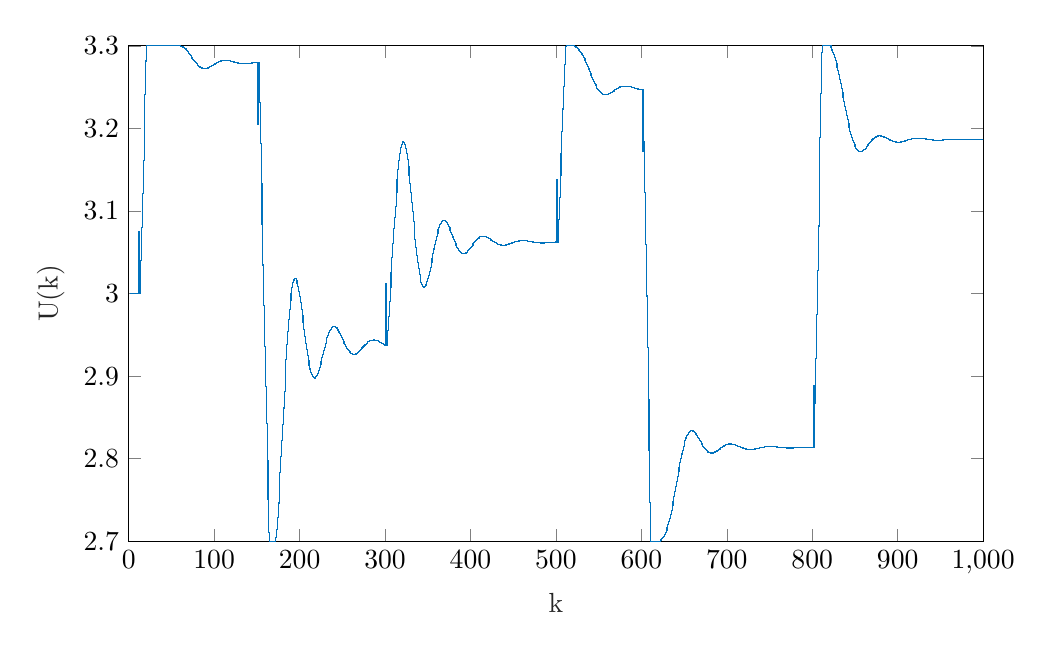
\begin{tikzpicture}

\begin{axis}[%
width=4.272in,
height=2.477in,
at={(0.717in,0.437in)},
scale only axis,
xmin=0,
xmax=1000,
xlabel style={font=\color{white!15!black}},
xlabel={k},
ymin=2.7,
ymax=3.3,
ylabel style={font=\color{white!15!black}},
ylabel={U(k)},
axis background/.style={fill=white}
]
\addplot[const plot, color=mycolor1, forget plot] table[row sep=crcr] {%
1	3\\
2	3\\
3	3\\
4	3\\
5	3\\
6	3\\
7	3\\
8	3\\
9	3\\
10	3\\
11	3\\
12	3.075\\
13	3\\
14	3.04022346368715\\
15	3.0804469273743\\
16	3.12067039106145\\
17	3.1608938547486\\
18	3.20111731843576\\
19	3.24134078212291\\
20	3.28156424581006\\
21	3.3\\
22	3.3\\
23	3.3\\
24	3.3\\
25	3.3\\
26	3.3\\
27	3.3\\
28	3.3\\
29	3.3\\
30	3.3\\
31	3.3\\
32	3.3\\
33	3.3\\
34	3.3\\
35	3.3\\
36	3.3\\
37	3.3\\
38	3.3\\
39	3.3\\
40	3.3\\
41	3.3\\
42	3.3\\
43	3.3\\
44	3.3\\
45	3.3\\
46	3.3\\
47	3.3\\
48	3.3\\
49	3.3\\
50	3.3\\
51	3.3\\
52	3.3\\
53	3.3\\
54	3.3\\
55	3.3\\
56	3.3\\
57	3.3\\
58	3.3\\
59	3.3\\
60	3.29988112356092\\
61	3.29960537447581\\
62	3.29918013626207\\
63	3.29861260841409\\
64	3.29790978875802\\
65	3.29707845982346\\
66	3.29612517869855\\
67	3.29505626989534\\
68	3.29387782080592\\
69	3.29259567937811\\
70	3.29122262708769\\
71	3.2897802191187\\
72	3.28829137369339\\
73	3.28677782580896\\
74	3.28526020435194\\
75	3.28375810294671\\
76	3.28229014506909\\
77	3.28087404391733\\
78	3.2795266574955\\
79	3.27826403932918\\
80	3.27710105233227\\
81	3.27605046259204\\
82	3.27512237945272\\
83	3.27432427107526\\
84	3.2736611136847\\
85	3.27313552491739\\
86	3.27274788330792\\
87	3.27249643570832\\
88	3.27237739421198\\
89	3.27238502395994\\
90	3.27251174915464\\
91	3.27274833396539\\
92	3.27308414696381\\
93	3.27350745452905\\
94	3.2740057028748\\
95	3.27456578291509\\
96	3.27517428051029\\
97	3.27581771424612\\
98	3.27648276256356\\
99	3.27715648176865\\
100	3.27782651462647\\
101	3.27848128419743\\
102	3.27911016380311\\
103	3.27970361682034\\
104	3.28025330551995\\
105	3.2807521707333\\
106	3.28119448420909\\
107	3.28157587516646\\
108	3.28189333225508\\
109	3.28214518188849\\
110	3.28233104381202\\
111	3.282451765079\\
112	3.28250933444183\\
113	3.28250678004186\\
114	3.28244805366707\\
115	3.28233790476837\\
116	3.28218174720573\\
117	3.28198552150343\\
118	3.2817555552468\\
119	3.28149842414471\\
120	3.28122081619766\\
121	3.28092940131798\\
122	3.28063070858935\\
123	3.28033101309572\\
124	3.28003623392152\\
125	3.27975184458201\\
126	3.27948279681786\\
127	3.27923345838831\\
128	3.27900756521539\\
129	3.27880818796406\\
130	3.27863771288358\\
131	3.27849783648466\\
132	3.27838957338713\\
133	3.27831327645563\\
134	3.27826866815356\\
135	3.27825488189485\\
136	3.27827051205724\\
137	3.27831367123768\\
138	3.27838205327778\\
139	3.27847300056277\\
140	3.2785835741005\\
141	3.27871062491687\\
142	3.27885086535927\\
143	3.27900093897945\\
144	3.27915748776799\\
145	3.2793172156315\\
146	3.27947694713622\\
147	3.27963368068498\\
148	3.27978463544515\\
149	3.27992729149924\\
150	3.28005942284611\\
151	3.20505942284611\\
152	3.28005942284611\\
153	3.23098789202009\\
154	3.18190027336593\\
155	3.13279604816791\\
156	3.08367503732403\\
157	3.03453738597983\\
158	2.98538354292902\\
159	2.93621423545881\\
160	2.88703044036518\\
161	2.84236632773794\\
162	2.79741713269406\\
163	2.75112559731369\\
164	2.71059404547725\\
165	2.7\\
166	2.7\\
167	2.7\\
168	2.7\\
169	2.7\\
170	2.7\\
171	2.7\\
172	2.70423842612691\\
173	2.71383154608654\\
174	2.72854349077787\\
175	2.74627865341111\\
176	2.76474874718158\\
177	2.78342353790016\\
178	2.80237072279201\\
179	2.82164579653832\\
180	2.84129358140333\\
181	2.86134958926031\\
182	2.88158547185606\\
183	2.90145891744165\\
184	2.92037635280685\\
185	2.93788208925374\\
186	2.95377413769652\\
187	2.96800667007094\\
188	2.98055280857674\\
189	2.99137204194431\\
190	3.00041261448197\\
191	3.00761359575016\\
192	3.01292210386222\\
193	3.01632782917861\\
194	3.01788422022003\\
195	3.01770313769924\\
196	3.01593188221605\\
197	3.01272977871366\\
198	3.0082588124201\\
199	3.00268407325409\\
200	2.99617582064833\\
201	2.9889111876953\\
202	2.98107464493438\\
203	2.97285533720264\\
204	2.96444114549923\\
205	2.95601186228509\\
206	2.94773405446038\\
207	2.93975861967187\\
208	2.9322201841119\\
209	2.92523693503241\\
210	2.91891023495921\\
211	2.9133239576476\\
212	2.90854365106439\\
213	2.90461579433911\\
214	2.90156752883515\\
215	2.8994071042761\\
216	2.89812498798721\\
217	2.89769537961265\\
218	2.8980778710274\\
219	2.89921912713208\\
220	2.90105458337985\\
221	2.9035101958777\\
222	2.90650427580246\\
223	2.90994941680094\\
224	2.91375448526847\\
225	2.91782660697972\\
226	2.92207307301857\\
227	2.92640310650737\\
228	2.93072946177397\\
229	2.9349698493402\\
230	2.93904818668204\\
231	2.94289567203664\\
232	2.94645167394225\\
233	2.9496644263557\\
234	2.95249152009227\\
235	2.95490018668319\\
236	2.95686737880783\\
237	2.95837965898665\\
238	2.95943291287964\\
239	2.96003190520652\\
240	2.96018969641536\\
241	2.95992693820411\\
242	2.95927106648144\\
243	2.95825541132661\\
244	2.95691824463704\\
245	2.95530178694737\\
246	2.95345119494612\\
247	2.9514135503851\\
248	2.94923686957597\\
249	2.94696915084146\\
250	2.94465747539097\\
251	2.94234717521356\\
252	2.94008107969129\\
253	2.93789885066957\\
254	2.93583641363421\\
255	2.93392549044487\\
256	2.93219323682112\\
257	2.9306619855635\\
258	2.92934909440167\\
259	2.92826689545014\\
260	2.92742274153775\\
261	2.92681914315935\\
262	2.92645398847501\\
263	2.92632083765768\\
264	2.9264092819748\\
265	2.92670535729761\\
266	2.92719200127257\\
267	2.92784954316482\\
268	2.92865621538467\\
269	2.9295886759188\\
270	2.93062253128804\\
271	2.9317328502226\\
272	2.93289465896308\\
273	2.9340834099413\\
274	2.93527541654785\\
275	2.93644824773111\\
276	2.93758107727127\\
277	2.93865498370796\\
278	2.93965319804783\\
279	2.94056129751559\\
280	2.94136734471743\\
281	2.94206197264176\\
282	2.94263841691095\\
283	2.94309249760561\\
284	2.94342255379742\\
285	2.94362933463703\\
286	2.9437158514432\\
287	2.94368719572189\\
288	2.94355032840823\\
289	2.94331384586806\\
290	2.94298772832375\\
291	2.94258307638269\\
292	2.94211184125431\\
293	2.94158655404992\\
294	2.94102005927696\\
295	2.94042525727754\\
296	2.93981485993016\\
297	2.93920116344582\\
298	2.93859584155728\\
299	2.93800976183595\\
300	2.93745282728634\\
301	3.01245282728634\\
302	2.93745282728634\\
303	2.95490838926636\\
304	2.97242085028363\\
305	2.98999387575159\\
306	3.00762979407033\\
307	3.02532962738992\\
308	3.04309314509237\\
309	3.06091893773032\\
310	3.07880450890349\\
311	3.09218931247435\\
312	3.10585448862715\\
313	3.12276590850344\\
314	3.137606607057\\
315	3.15038901012984\\
316	3.16111930903239\\
317	3.16979843201349\\
318	3.17642291518366\\
319	3.18098568077976\\
320	3.18347672989019\\
321	3.18415874506739\\
322	3.18326146254501\\
323	3.180559596438\\
324	3.17598116182379\\
325	3.16975666704132\\
326	3.16211272785718\\
327	3.15327362676779\\
328	3.14346263223078\\
329	3.13290310665972\\
330	3.12181942891035\\
331	3.11042116047239\\
332	3.09889000088873\\
333	3.08740966222041\\
334	3.07618272501215\\
335	3.06540360058475\\
336	3.05524172771909\\
337	3.04584224802211\\
338	3.03732640878614\\
339	3.0297917365226\\
340	3.02331201864886\\
341	3.01793812713455\\
342	3.01370047330709\\
343	3.01061034067137\\
344	3.00865845605576\\
345	3.00781422409752\\
346	3.00802750648531\\
347	3.00923128688642\\
348	3.0113442418281\\
349	3.01427325810047\\
350	3.01791593057356\\
351	3.02216300817539\\
352	3.0269006483517\\
353	3.03201246158384\\
354	3.03738158238336\\
355	3.04289288671449\\
356	3.04843516531731\\
357	3.05390305678101\\
358	3.05919869914257\\
359	3.06423311153506\\
360	3.06892731189592\\
361	3.07321317582169\\
362	3.07703405113423\\
363	3.08034515105141\\
364	3.08311373494777\\
365	3.08531906453723\\
366	3.08695212781236\\
367	3.08801514561296\\
368	3.08852088903709\\
369	3.08849183719737\\
370	3.08795920354172\\
371	3.08696185816089\\
372	3.08554517228369\\
373	3.08375980897887\\
374	3.08166048234404\\
375	3.07930470785138\\
376	3.07675156787336\\
377	3.07406051616165\\
378	3.07129024273896\\
379	3.0684976175491\\
380	3.0657367281357\\
381	3.0630580236885\\
382	3.06050757499511\\
383	3.05812645723793\\
384	3.0559502601996\\
385	3.05400872812489\\
386	3.05232552904935\\
387	3.05091815088342\\
388	3.04979791915052\\
389	3.04897012918129\\
390	3.04843428380182\\
391	3.04818442610863\\
392	3.04820955577887\\
393	3.04849411649996\\
394	3.04901854149482\\
395	3.04975984375133\\
396	3.05069223744311\\
397	3.05178777716813\\
398	3.05301700203018\\
399	3.05434957222352\\
400	3.05575488661982\\
401	3.05720267086263\\
402	3.05866352661662\\
403	3.06010943386577\\
404	3.06151419947867\\
405	3.06285384663542\\
406	3.06410694111339\\
407	3.06525485183282\\
408	3.06628194443924\\
409	3.0671757080232\\
410	3.06792681632451\\
411	3.06852912591911\\
412	3.06897961492574\\
413	3.06927826668488\\
414	3.06942790364306\\
415	3.06943397731648\\
416	3.06930432070321\\
417	3.06904886986253\\
418	3.06867936158374\\
419	3.06820901412976\\
420	3.06765219796931\\
421	3.06702410321418\\
422	3.0663404101669\\
423	3.06561696896956\\
424	3.06486949384217\\
425	3.06411327682069\\
426	3.06336292526803\\
427	3.06263212674892\\
428	3.06193344414861\\
429	3.06127814318929\\
430	3.06067605377281\\
431	3.06013546586581\\
432	3.05966305995784\\
433	3.0592638714743\\
434	3.05894128792567\\
435	3.05869707702936\\
436	3.05853144355953\\
437	3.05844311226713\\
438	3.05842943387264\\
439	3.05848651086861\\
440	3.0586093396798\\
441	3.05879196561452\\
442	3.05902764699935\\
443	3.05930902491807\\
444	3.0596282950695\\
445	3.0599773784128\\
446	3.06034808747622\\
447	3.0607322854603\\
448	3.06112203555987\\
449	3.0615097382558\\
450	3.06188825467674\\
451	3.06225101449747\\
452	3.06259210721459\\
453	3.06290635601554\\
454	3.06318937382608\\
455	3.06343760147758\\
456	3.06364832827317\\
457	3.0638196955455\\
458	3.06395068408384\\
459	3.06404108656153\\
460	3.06409146631213\\
461	3.06410310398328\\
462	3.06407793373904\\
463	3.06401847078416\\
464	3.06392773204743\\
465	3.06380915188744\\
466	3.06366649467347\\
467	3.06350376604986\\
468	3.06332512461652\\
469	3.06313479565408\\
470	3.06293698839359\\
471	3.06273581818117\\
472	3.0625352347214\\
473	3.06233895740377\\
474	3.06215041852845\\
475	3.06197271505439\\
476	3.06180856929894\\
477	3.0616602988268\\
478	3.06152979558119\\
479	3.06141851413421\\
480	3.06132746876976\\
481	3.06125723896305\\
482	3.06120798268788\\
483	3.06117945686826\\
484	3.06117104419494\\
485	3.06118178545199\\
486	3.06121041644286\\
487	3.06125540856979\\
488	3.06131501210485\\
489	3.06138730119391\\
490	3.06147021965545\\
491	3.06156162667372\\
492	3.06165934153741\\
493	3.06176118664017\\
494	3.06186502803529\\
495	3.06196881292184\\
496	3.06207060353164\\
497	3.06216860698311\\
498	3.06226120076766\\
499	3.06234695363444\\
500	3.06242464173843\\
501	3.13742464173843\\
502	3.06242464173843\\
503	3.08928865138536\\
504	3.11614193245399\\
505	3.14298437678019\\
506	3.16981608487126\\
507	3.19663735243959\\
508	3.22344865403322\\
509	3.25025062423074\\
510	3.27704403688747\\
511	3.29930817085649\\
512	3.3\\
513	3.3\\
514	3.3\\
515	3.3\\
516	3.3\\
517	3.3\\
518	3.3\\
519	3.3\\
520	3.3\\
521	3.3\\
522	3.29928094616488\\
523	3.29850712450603\\
524	3.29767851052772\\
525	3.29676165132026\\
526	3.29572882721796\\
527	3.29455734341882\\
528	3.2932288988898\\
529	3.29172902465614\\
530	3.29004658434979\\
531	3.28817333059442\\
532	3.28614690157086\\
533	3.28400764205772\\
534	3.28175956407363\\
535	3.27941044171693\\
536	3.2769730991866\\
537	3.27446452891859\\
538	3.27190513002111\\
539	3.26931805169573\\
540	3.26672862821406\\
541	3.26416389367753\\
542	3.26164954794001\\
543	3.25920711482412\\
544	3.25685594862934\\
545	3.25461502661005\\
546	3.25250236215837\\
547	3.2505344100929\\
548	3.24872557847926\\
549	3.24708783085668\\
550	3.24563036508968\\
551	3.24435935707954\\
552	3.24327791729898\\
553	3.24238639164692\\
554	3.24168270023402\\
555	3.24116245115929\\
556	3.24081898813969\\
557	3.24064350912775\\
558	3.24062524938453\\
559	3.24075171715093\\
560	3.24100897205014\\
561	3.24138193802068\\
562	3.24185473443779\\
563	3.24241099286132\\
564	3.24303413808573\\
565	3.24370764558211\\
566	3.24441529256297\\
567	3.2451414022931\\
568	3.24587107378979\\
569	3.24659039016639\\
570	3.24728660014294\\
571	3.24794826828144\\
572	3.24856539091913\\
573	3.24912947761909\\
574	3.24963360102787\\
575	3.25007241842773\\
576	3.25044216646579\\
577	3.25074062954118\\
578	3.25096708280381\\
579	3.25112221155452\\
580	3.25120800953031\\
581	3.25122765912123\\
582	3.25118539698675\\
583	3.25108636871489\\
584	3.2509364760024\\
585	3.25074221948018\\
586	3.25051054005006\\
587	3.25024866151129\\
588	3.24996393720013\\
589	3.24966370323538\\
590	3.24935514074616\\
591	3.24904514916996\\
592	3.24874023236546\\
593	3.24844639890837\\
594	3.24816907756297\\
595	3.24791304857684\\
596	3.24768239113604\\
597	3.24748044702542\\
598	3.24730980025152\\
599	3.24717227210643\\
600	3.24706893088887\\
601	3.17206893088887\\
602	3.24706893088887\\
603	3.18449762139125\\
604	3.12195788702798\\
605	3.05944760828419\\
606	2.99696420962688\\
607	2.93450473458795\\
608	2.87206592376911\\
609	2.80964429414009\\
610	2.74723621806741\\
611	2.7\\
612	2.7\\
613	2.7\\
614	2.7\\
615	2.7\\
616	2.7\\
617	2.7\\
618	2.7\\
619	2.7\\
620	2.7\\
621	2.7\\
622	2.70097469693636\\
623	2.70198540390985\\
624	2.70312451700154\\
625	2.7044693352988\\
626	2.70608389866669\\
627	2.70802062644267\\
628	2.71032177732435\\
629	2.71302074873268\\
630	2.7161432321357\\
631	2.71970823919288\\
632	2.72367019561329\\
633	2.72798011220069\\
634	2.73263307979809\\
635	2.73761041110359\\
636	2.74288196284304\\
637	2.74840814349479\\
638	2.75414164649143\\
639	2.7600289439227\\
640	2.76601157144824\\
641	2.77202723133033\\
642	2.77801428634013\\
643	2.78391579804356\\
644	2.78967715940553\\
645	2.79524452827017\\
646	2.80056642744242\\
647	2.80559506444796\\
648	2.81028741335419\\
649	2.81460609487705\\
650	2.81852008570281\\
651	2.8220052834043\\
652	2.82504473525675\\
653	2.82762836864518\\
654	2.82975263969213\\
655	2.83142041633746\\
656	2.83264085532287\\
657	2.8334291085451\\
658	2.83380588992113\\
659	2.83379692866085\\
660	2.83343233044866\\
661	2.83274586436327\\
662	2.83177420322565\\
663	2.83055616556932\\
664	2.82913199121963\\
665	2.82754263955601\\
666	2.82582909639026\\
667	2.82403169940101\\
668	2.82218949964765\\
669	2.82033967336364\\
670	2.81851699552653\\
671	2.81675338451069\\
672	2.81507752457453\\
673	2.81351456859915\\
674	2.81208591899553\\
675	2.8108090837288\\
676	2.80969760605307\\
677	2.8087610668787\\
678	2.80800515716753\\
679	2.80743181598633\\
680	2.80703942842844\\
681	2.80682307646857\\
682	2.8067748349335\\
683	2.80688410427945\\
684	2.80713797187339\\
685	2.80752159377484\\
686	2.80801858924818\\
687	2.80861144033801\\
688	2.80928188900232\\
689	2.8100113246438\\
690	2.81078115540034\\
691	2.8115731572178\\
692	2.81236979550086\\
693	2.81315451498422\\
694	2.81391199433707\\
695	2.81462836286421\\
696	2.81529137748779\\
697	2.81589055899734\\
698	2.81641728734936\\
699	2.81686485656667\\
700	2.81722849051345\\
701	2.817505321486\\
702	2.81769433414816\\
703	2.81779627784507\\
704	2.81781355074245\\
705	2.81775005956304\\
706	2.81761105892884\\
707	2.81740297447085\\
708	2.81713321393729\\
709	2.81680997051944\\
710	2.81644202252372\\
711	2.81603853335504\\
712	2.81560885554731\\
713	2.81516234229006\\
714	2.81470816956532\\
715	2.81425517163443\\
716	2.81381169221173\\
717	2.81338545323705\\
718	2.81298344272312\\
719	2.81261182271426\\
720	2.81227585795775\\
721	2.81197986546789\\
722	2.81172718476065\\
723	2.81152016816226\\
724	2.81136019025215\\
725	2.81124767519469\\
726	2.81118214044891\\
727	2.81116225512242\\
728	2.8111859110586\\
729	2.81125030461371\\
730	2.81135202699419\\
731	2.81148716098279\\
732	2.81165138188323\\
733	2.81184006055505\\
734	2.81204836648947\\
735	2.8122713689905\\
736	2.81250413466861\\
737	2.81274181962319\\
738	2.81297975487949\\
739	2.81321352385222\\
740	2.81343903082514\\
741	2.81365255966078\\
742	2.81385082218079\\
743	2.814030995882\\
744	2.8141907508718\\
745	2.81432826611443\\
746	2.81444223527519\\
747	2.81453186262814\\
748	2.81459684965341\\
749	2.81463737308932\\
750	2.81465405532261\\
751	2.81464792809411\\
752	2.81462039056828\\
753	2.81457316286241\\
754	2.81450823615541\\
755	2.81442782049817\\
756	2.81433429142832\\
757	2.81423013645314\\
758	2.81411790240843\\
759	2.81400014462844\\
760	2.81387937877643\\
761	2.81375803608874\\
762	2.81363842267942\\
763	2.81352268344078\\
764	2.81341277095972\\
765	2.81331041975247\\
766	2.81321712600416\\
767	2.81313413288656\\
768	2.81306242141872\\
769	2.81300270673382\\
770	2.81295543952177\\
771	2.81292081233346\\
772	2.81289877035877\\
773	2.81288902622854\\
774	2.8128910783404\\
775	2.81290423217021\\
776	2.81292762400484\\
777	2.81296024651825\\
778	2.81300097561038\\
779	2.81304859793683\\
780	2.8131018385764\\
781	2.81315938831157\\
782	2.81321993003325\\
783	2.81328216382496\\
784	2.81334483033063\\
785	2.8134067320646\\
786	2.81346675237955\\
787	2.81352387186795\\
788	2.81357718203284\\
789	2.81362589612408\\
790	2.81366935709491\\
791	2.81370704269003\\
792	2.81373856772943\\
793	2.8137636837011\\
794	2.81378227581973\\
795	2.81379435774721\\
796	2.81380006420359\\
797	2.81379964172394\\
798	2.81379343783691\\
799	2.81378188895516\\
800	2.81376550727567\\
801	2.88876550727567\\
802	2.81376550727567\\
803	2.86736953422179\\
804	2.92097125500743\\
805	2.97457135024748\\
806	3.02817049320379\\
807	3.08176933759933\\
808	3.13536850647461\\
809	3.18896858223666\\
810	3.24257009802065\\
811	3.29164653221768\\
812	3.3\\
813	3.3\\
814	3.3\\
815	3.3\\
816	3.3\\
817	3.3\\
818	3.3\\
819	3.3\\
820	3.3\\
821	3.3\\
822	3.29772923274357\\
823	3.29496367997889\\
824	3.29210096757155\\
825	3.28906999988931\\
826	3.28581174240889\\
827	3.28227773609557\\
828	3.27842877362799\\
829	3.27423372093537\\
830	3.26966846913828\\
831	3.26471500345344\\
832	3.25949760269862\\
833	3.25416626966239\\
834	3.24874854408035\\
835	3.24325737301135\\
836	3.23771676972946\\
837	3.2321599054427\\
838	3.22662745992251\\
839	3.22116619823445\\
840	3.21582774477811\\
841	3.21066752938426\\
842	3.20573561473755\\
843	3.20106689883863\\
844	3.19668700052872\\
845	3.19262001528921\\
846	3.18888849536096\\
847	3.18551210049998\\
848	3.18250648693556\\
849	3.17988239883156\\
850	3.17764493169269\\
851	3.17579294158451\\
852	3.1743190767967\\
853	3.17321092587382\\
854	3.17245236179023\\
855	3.1720240762029\\
856	3.17190367693606\\
857	3.17206587721638\\
858	3.17248283671494\\
859	3.17312462690554\\
860	3.17395979778628\\
861	3.17495602682078\\
862	3.17608080404207\\
863	3.1773020507774\\
864	3.1785885976721\\
865	3.17991056124878\\
866	3.18123969229453\\
867	3.18254971522113\\
868	3.18381664352447\\
869	3.18501905483027\\
870	3.18613831207324\\
871	3.18715871986385\\
872	3.1880676089641\\
873	3.18885535055802\\
874	3.18951531220821\\
875	3.19004376906675\\
876	3.19043977708628\\
877	3.19070500958759\\
878	3.19084355836408\\
879	3.19086170237471\\
880	3.19076764884403\\
881	3.19057125302199\\
882	3.19028372391286\\
883	3.18991732359414\\
884	3.18948506695452\\
885	3.18900042722417\\
886	3.18847705155327\\
887	3.18792849050458\\
888	3.18736794525637\\
889	3.18680803613822\\
890	3.18626059573296\\
891	3.18573648920201\\
892	3.18524546376964\\
893	3.18479602850149\\
894	3.18439536474123\\
895	3.1840492669287\\
896	3.18376211302742\\
897	3.18353686337399\\
898	3.18337508636542\\
899	3.18327700900973\\
900	3.18324159000096\\
901	3.18326661266358\\
902	3.1833487948648\\
903	3.1834839128276\\
904	3.18366693569599\\
905	3.18389216769788\\
906	3.18415339480322\\
907	3.18444403287413\\
908	3.18475727444461\\
909	3.1850862314484\\
910	3.18542407143552\\
911	3.18576414507521\\
912	3.18610010303077\\
913	3.18642600060169\\
914	3.18673638885124\\
915	3.18702639126522\\
916	3.18729176531293\\
917	3.18752894859888\\
918	3.18773508959884\\
919	3.18790806326279\\
920	3.18804647203511\\
921	3.18814963308579\\
922	3.18821755276145\\
923	3.18825088944867\\
924	3.18825090619331\\
925	3.18821941453648\\
926	3.18815871111083\\
927	3.18807150859047\\
928	3.18796086260491\\
929	3.18783009621349\\
930	3.18768272349391\\
931	3.18752237372856\\
932	3.18735271757901\\
933	3.18717739652419\\
934	3.18699995670576\\
935	3.18682378817812\\
936	3.18665207040356\\
937	3.18648772466966\\
938	3.18633337393853\\
939	3.18619131047012\\
940	3.18606347139717\\
941	3.18595142227054\\
942	3.18585634844332\\
943	3.18577905402263\\
944	3.18571996799126\\
945	3.18567915698902\\
946	3.18565634414744\\
947	3.18565093329151\\
948	3.18566203775975\\
949	3.18568851304907\\
950	3.18572899246297\\
951	3.18578192493114\\
952	3.18584561417387\\
953	3.18591825840518\\
954	3.18599798980336\\
955	3.18608291302444\\
956	3.18617114209221\\
957	3.18626083506578\\
958	3.18635022596015\\
959	3.18643765347592\\
960	3.18652158617841\\
961	3.18660064385266\\
962	3.18667361484761\\
963	3.18673946930801\\
964	3.18679736827503\\
965	3.18684666871478\\
966	3.18688692460714\\
967	3.18691788429299\\
968	3.18693948433733\\
969	3.18695184021665\\
970	3.18695523418062\\
971	3.18695010067229\\
972	3.18693700971475\\
973	3.18691664868777\\
974	3.18688980292454\\
975	3.18685733555681\\
976	3.18682016702682\\
977	3.18677925466773\\
978	3.18673557273039\\
979	3.18669009320498\\
980	3.18664376775211\\
981	3.18659751101934\\
982	3.18655218557823\\
983	3.18650858867338\\
984	3.18646744093064\\
985	3.18642937712662\\
986	3.18639493907769\\
987	3.18636457066349\\
988	3.18633861495957\\
989	3.18631731341536\\
990	3.18630080697929\\
991	3.18628913904185\\
992	3.18628226004031\\
993	3.18628003354688\\
994	3.18628224364377\\
995	3.18628860337589\\
996	3.18629876406306\\
997	3.18631232524984\\
998	3.18632884507141\\
999	3.18634785081857\\
1000	3.18636884949305\\
};
\end{axis}
\end{tikzpicture}%
\caption{Sterowanie PID dla parametrów $K=1,6$, $T_i=8,95$,  $T_d=3,05$}
\end{figure}

\begin{figure}[H]
\centering
% This file was created by matlab2tikz.
%
%The latest updates can be retrieved from
%  http://www.mathworks.com/matlabcentral/fileexchange/22022-matlab2tikz-matlab2tikz
%where you can also make suggestions and rate matlab2tikz.
%
\definecolor{mycolor1}{rgb}{0.00000,0.44700,0.74100}%
\definecolor{mycolor2}{rgb}{0.85000,0.32500,0.09800}%
%
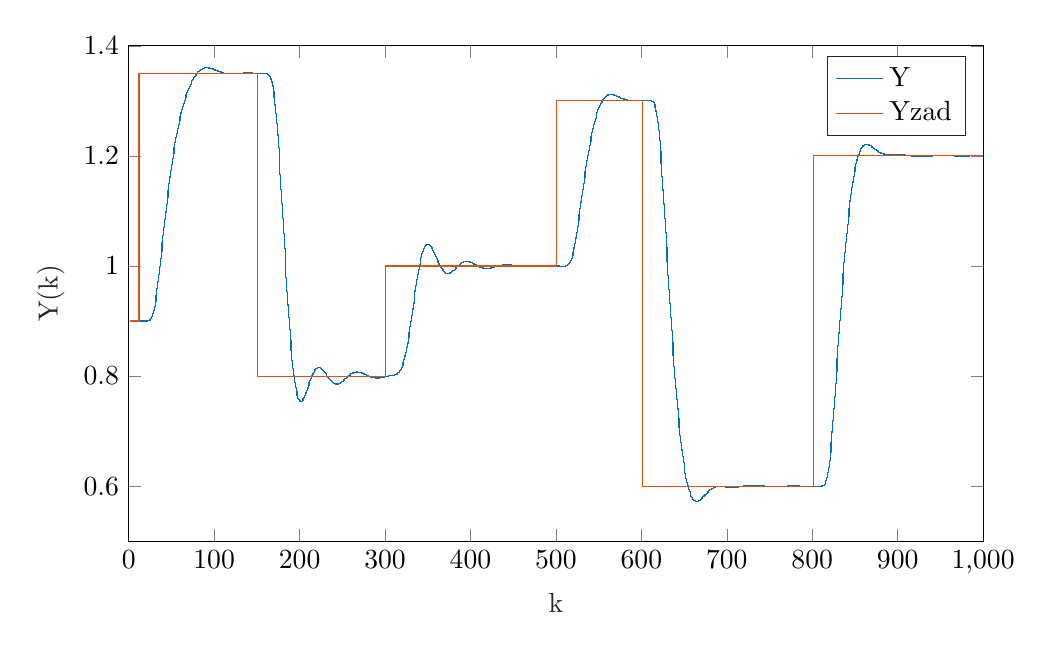
\begin{tikzpicture}

\begin{axis}[%
width=4.272in,
height=2.477in,
at={(0.717in,0.437in)},
scale only axis,
xmin=0,
xmax=1000,
xlabel style={font=\color{white!15!black}},
xlabel={k},
ymin=0.5,
ymax=1.4,
ylabel style={font=\color{white!15!black}},
ylabel={Y(k)},
axis background/.style={fill=white},
legend style={legend cell align=left, align=left, draw=white!15!black}
]
\addplot[const plot, color=mycolor1] table[row sep=crcr] {%
1	0.9\\
2	0.9\\
3	0.9\\
4	0.9\\
5	0.9\\
6	0.9\\
7	0.9\\
8	0.9\\
9	0.9\\
10	0.9\\
11	0.9\\
12	0.9\\
13	0.9\\
14	0.9\\
15	0.9\\
16	0.9\\
17	0.9\\
18	0.9\\
19	0.9\\
20	0.9\\
21	0.9\\
22	0.9003968325\\
23	0.90110505465075\\
24	0.901909610498159\\
25	0.903204539730905\\
26	0.905319864516099\\
27	0.908529368064496\\
28	0.913057531336706\\
29	0.919085713562694\\
30	0.926757653850088\\
31	0.936069082613075\\
32	0.946799343503458\\
33	0.958660553287854\\
34	0.971402068619519\\
35	0.984806336593277\\
36	0.998685174610892\\
37	1.01287643703728\\
38	1.02724103022174\\
39	1.04166024116579\\
40	1.05603334847553\\
41	1.07027548727566\\
42	1.08431574251261\\
43	1.09809544756337\\
44	1.11156666731939\\
45	1.12469084695225\\
46	1.13743760941134\\
47	1.14978368637027\\
48	1.16171196884628\\
49	1.17321066507913\\
50	1.18427255448749\\
51	1.19489432763354\\
52	1.20507600313168\\
53	1.21482041334531\\
54	1.22413275153552\\
55	1.23302017386552\\
56	1.24149145033279\\
57	1.24955665930374\\
58	1.25722692086914\\
59	1.26451416472911\\
60	1.27143092875846\\
61	1.27799018480122\\
62	1.28420518860264\\
63	1.29008935110969\\
64	1.29565612866229\\
65	1.30091892985958\\
66	1.30589103712079\\
67	1.31058554117257\\
68	1.31501528688484\\
69	1.3191928290485\\
70	1.32312976785484\\
71	1.32683602633562\\
72	1.33031989494113\\
73	1.33358830574958\\
74	1.33664707101705\\
75	1.33950108989007\\
76	1.34215452675512\\
77	1.34461096437699\\
78	1.34687353468147\\
79	1.34894502976416\\
80	1.35082803341134\\
81	1.35252511474642\\
82	1.35403904316049\\
83	1.35537296931337\\
84	1.35653056395735\\
85	1.35751612097242\\
86	1.35833463018169\\
87	1.35899182479253\\
88	1.35949420767133\\
89	1.35984906009754\\
90	1.36006443385884\\
91	1.36014912258497\\
92	1.36011260821474\\
93	1.35996498406169\\
94	1.35971685945396\\
95	1.35937925085749\\
96	1.35896346356733\\
97	1.35848096734741\\
98	1.35794326880009\\
99	1.35736178273701\\
100	1.35674770452899\\
101	1.35611188558833\\
102	1.35546471460074\\
103	1.35481600725403\\
104	1.35417490681695\\
105	1.35354979734037\\
106	1.35294823073563\\
107	1.35237686856272\\
108	1.35184143901963\\
109	1.35134670934957\\
110	1.35089647365482\\
111	1.35049355588431\\
112	1.35013982750049\\
113	1.34983623903446\\
114	1.34958286445712\\
115	1.3493789570682\\
116	1.34922301544164\\
117	1.34911285785405\\
118	1.3490457035524\\
119	1.34901825917945\\
120	1.34902680866331\\
121	1.34906730488908\\
122	1.34913546150719\\
123	1.34922684330011\\
124	1.34933695362757\\
125	1.34946131759624\\
126	1.34959555974692\\
127	1.34973547521338\\
128	1.34987709347847\\
129	1.35001673402933\\
130	1.35015105339357\\
131	1.35027708321722\\
132	1.35039225922342\\
133	1.35049444106224\\
134	1.35058192322619\\
135	1.35065343735758\\
136	1.35070814641164\\
137	1.35074563126053\\
138	1.35076587042752\\
139	1.35076921372609\\
140	1.35075635064585\\
141	1.3507282743751\\
142	1.35068624237942\\
143	1.35063173446648\\
144	1.35056640926032\\
145	1.35049205998536\\
146	1.35041057042091\\
147	1.35032387183528\\
148	1.35023390164342\\
149	1.35014256445793\\
150	1.3500516961204\\
151	1.34996303121129\\
152	1.34987817444316\\
153	1.34979857624708\\
154	1.34972551276574\\
155	1.349660070373\\
156	1.34960313474779\\
157	1.34955538444407\\
158	1.34951728881764\\
159	1.34948911009717\\
160	1.34947090932144\\
161	1.34906508996251\\
162	1.34835572883538\\
163	1.3475098606777\\
164	1.3460487471998\\
165	1.34357138439032\\
166	1.33974505545299\\
167	1.33429690969128\\
168	1.32700646254125\\
169	1.31769892219885\\
170	1.30623925756315\\
171	1.29255091504119\\
172	1.27660453658434\\
173	1.25838122261118\\
174	1.23790332656466\\
175	1.21539139829565\\
176	1.19125076799511\\
177	1.16588757016083\\
178	1.13965301594292\\
179	1.11284963104965\\
180	1.08573684148366\\
181	1.05853597212013\\
182	1.03145714278817\\
183	1.00472676666125\\
184	0.978587920794745\\
185	0.953283947697651\\
186	0.929034264633752\\
187	0.906022401522852\\
188	0.884398076269026\\
189	0.864282092853132\\
190	0.845770550198537\\
191	0.828938456221019\\
192	0.813841475798337\\
193	0.800514551116716\\
194	0.788969025747339\\
195	0.779190837173562\\
196	0.771141183385443\\
197	0.764759340391656\\
198	0.759966066299063\\
199	0.756666620652464\\
200	0.75475328877083\\
201	0.754107494306025\\
202	0.754601651608476\\
203	0.756101055084415\\
204	0.758466072563334\\
205	0.761554659379839\\
206	0.765224979233694\\
207	0.769337859728288\\
208	0.773758925715462\\
209	0.778360402073334\\
210	0.783022638600583\\
211	0.78763540954841\\
212	0.792099025271777\\
213	0.796325266142354\\
214	0.800238115463158\\
215	0.803774251928632\\
216	0.806883274302788\\
217	0.809527659618421\\
218	0.811682480923327\\
219	0.813334919630814\\
220	0.814483604449905\\
221	0.815137802475823\\
222	0.815316482707941\\
223	0.8150472695793\\
224	0.814365305047783\\
225	0.813312041673782\\
226	0.811933993172406\\
227	0.810281470571156\\
228	0.808407330646814\\
229	0.806365759952536\\
230	0.804211114109817\\
231	0.801996829008469\\
232	0.799774418235339\\
233	0.797592569201882\\
234	0.795496348680344\\
235	0.793526526398715\\
236	0.791719022807336\\
237	0.790104484250626\\
238	0.788707985879393\\
239	0.787548860009879\\
240	0.786640645393914\\
241	0.785991150983515\\
242	0.785602626171557\\
243	0.785472028096908\\
244	0.785591375384875\\
245	0.785948176665473\\
246	0.786525921419583\\
247	0.787304620195413\\
248	0.788261381036306\\
249	0.789371009052007\\
250	0.790606616412182\\
251	0.791940230602008\\
252	0.793343389520737\\
253	0.794787712900279\\
254	0.796245440553269\\
255	0.797689929110816\\
256	0.799096100157947\\
257	0.800440833992283\\
258	0.801703304587563\\
259	0.802865252706392\\
260	0.803911195447072\\
261	0.804828571803105\\
262	0.805607825040373\\
263	0.806242423838915\\
264	0.806728825188362\\
265	0.807066382955302\\
266	0.807257206845474\\
267	0.807305977155082\\
268	0.807219721237622\\
269	0.807007558003117\\
270	0.806680417016188\\
271	0.806250738871669\\
272	0.805732163507174\\
273	0.805139212969317\\
274	0.804486974893381\\
275	0.803790792596432\\
276	0.80306596723331\\
277	0.802327476937104\\
278	0.801589717274848\\
279	0.800866266709818\\
280	0.800169680088797\\
281	0.799511312480509\\
282	0.798901174994099\\
283	0.798347823517442\\
284	0.797858280646532\\
285	0.797437990440682\\
286	0.797090805043813\\
287	0.796819001668582\\
288	0.796623327954823\\
289	0.796503073292686\\
290	0.796456163348142\\
291	0.796479274747136\\
292	0.796567966665843\\
293	0.796716825938018\\
294	0.796919622225056\\
295	0.797169469797164\\
296	0.797458992541307\\
297	0.79778048893844\\
298	0.798126093933286\\
299	0.79848793484822\\
300	0.798858278761749\\
301	0.79922966907436\\
302	0.799595049312616\\
303	0.799947872568758\\
304	0.800282195330248\\
305	0.80059275481433\\
306	0.800875029279898\\
307	0.801125281136254\\
308	0.801340582999747\\
309	0.801518827159462\\
310	0.801658719197553\\
311	0.802159335252828\\
312	0.802940147021879\\
313	0.803669986195597\\
314	0.804532050919438\\
315	0.805680994111689\\
316	0.807246374580988\\
317	0.809335721947638\\
318	0.812037255857431\\
319	0.815422296155624\\
320	0.819547397198662\\
321	0.824432124378659\\
322	0.830067123866269\\
323	0.836458264216281\\
324	0.843610953203256\\
325	0.851503638309168\\
326	0.860092204952541\\
327	0.869313780548394\\
328	0.879090021320756\\
329	0.889329949222156\\
330	0.899932397871368\\
331	0.910789573968912\\
332	0.921791300843777\\
333	0.932826049221194\\
334	0.943780351957509\\
335	0.954540689118354\\
336	0.964996574988397\\
337	0.9750431168982\\
338	0.98458312587763\\
339	0.993528847333345\\
340	1.00180336980477\\
341	1.0093416733565\\
342	1.01609121833379\\
343	1.02201223453097\\
344	1.02707799386303\\
345	1.03127500861839\\
346	1.03460294133887\\
347	1.0370741909601\\
348	1.03871321338954\\
349	1.03955562483349\\
350	1.03964712794846\\
351	1.03904229932948\\
352	1.03780328462842\\
353	1.03599844325863\\
354	1.0337009582569\\
355	1.03098741438355\\
356	1.02793636405215\\
357	1.02462691514951\\
358	1.02113737333786\\
359	1.0175439652934\\
360	1.01391966435911\\
361	1.01033313574367\\
362	1.00684781371356\\
363	1.00352111838865\\
364	1.0004038167721\\
365	0.99753953191384\\
366	0.994964403055952\\
367	0.992706896709899\\
368	0.990787764966088\\
369	0.989220144128907\\
370	0.988009784192249\\
371	0.987155397608443\\
372	0.986649114236367\\
373	0.986477028307528\\
374	0.986619822616249\\
375	0.987053454680592\\
376	0.987749889228199\\
377	0.988677861169964\\
378	0.989803653387753\\
379	0.991091874198037\\
380	0.992506220199991\\
381	0.994010211310237\\
382	0.995567886071386\\
383	0.997144446742339\\
384	0.998706845184892\\
385	1.00022430212386\\
386	1.00166875396727\\
387	1.00301522301692\\
388	1.00424210854891\\
389	1.00533139785818\\
390	1.00626879790524\\
391	1.00704378964578\\
392	1.00764960844285\\
393	1.00808315513884\\
394	1.00834484339001\\
395	1.00843838973189\\
396	1.00837055354497\\
397	1.00815083462132\\
398	1.00779113639232\\
399	1.00730540306639\\
400	1.00670923894904\\
401	1.00601951808424\\
402	1.00525399207861\\
403	1.00443090356083\\
404	1.00356861220483\\
405	1.0026852396213\\
406	1.00179833871614\\
407	1.0009245923432\\
408	1.00007954526005\\
409	0.999277372547726\\
410	0.998530686795498\\
411	0.997850385497035\\
412	0.997245539270544\\
413	0.99672332071661\\
414	0.996288972977052\\
415	0.995945816366966\\
416	0.995695290830002\\
417	0.995537031421498\\
418	0.995468973561422\\
419	0.995487484423075\\
420	0.995587516536531\\
421	0.99576277948821\\
422	0.996005925488462\\
423	0.996308744554801\\
424	0.996662365115084\\
425	0.997057455966953\\
426	0.997484425730602\\
427	0.997933616193764\\
428	0.998395486262499\\
429	0.998860783590072\\
430	0.999320701349728\\
431	0.999767018036275\\
432	1.00019221861675\\
433	1.00058959579306\\
434	1.00095333058057\\
435	1.00127855183828\\
436	1.00156137480037\\
437	1.00179891904965\\
438	1.00198930673337\\
439	1.00213164214806\\
440	1.00222597410556\\
441	1.00227324273702\\
442	1.00227521259077\\
443	1.00223439403348\\
444	1.00215395507177\\
445	1.00203762577321\\
446	1.00188959748314\\
447	1.00171441900973\\
448	1.00151689188565\\
449	1.00130196671539\\
450	1.00107464248531\\
451	1.00083987055442\\
452	1.0006024648607\\
453	1.00036701967677\\
454	1.00013783603334\\
455	0.99991885770501\\
456	0.999713617424419\\
457	0.999525193762523\\
458	0.999356178889276\\
459	0.999208657213452\\
460	0.999084194697139\\
461	0.99898383845214\\
462	0.998908126055117\\
463	0.998857103867811\\
464	0.998830353519959\\
465	0.998827025606626\\
466	0.998845879569459\\
467	0.998885328672908\\
468	0.998943488951676\\
469	0.999018230993797\\
470	0.99910723343374\\
471	0.999208037060474\\
472	0.999318098494746\\
473	0.999434842455907\\
474	0.999555711719413\\
475	0.999678213959235\\
476	0.999799964772356\\
477	0.999918726293003\\
478	1.00003244091959\\
479	1.00013925979526\\
480	1.00023756580085\\
481	1.00032599093536\\
482	1.00040342807056\\
483	1.0004690371726\\
484	1.00052224618162\\
485	1.0005627468298\\
486	1.0005904857571\\
487	1.00060565135232\\
488	1.00060865680292\\
489	1.00060011988125\\
490	1.00058084002666\\
491	1.00055177330226\\
492	1.00051400581283\\
493	1.00046872616653\\
494	1.00041719754866\\
495	1.00036072995126\\
496	1.00030065306939\\
497	1.00023829033395\\
498	1.0001749345037\\
499	1.00011182518632\\
500	1.00005012860183\\
501	0.999990919842462\\
502	0.99993516782201\\
503	0.999883723046869\\
504	0.999837308280823\\
505	0.99979651211745\\
506	0.999761785418924\\
507	0.999733440528636\\
508	0.999711653118355\\
509	0.99969646648906\\
510	0.999687798108787\\
511	1.00008191757482\\
512	1.00079247930032\\
513	1.00153294552259\\
514	1.0025704464216\\
515	1.00412882852705\\
516	1.00639390941521\\
517	1.00951816601721\\
518	1.01362491388677\\
519	1.01881202914533\\
520	1.02515525973664\\
521	1.03268724372746\\
522	1.04129116647226\\
523	1.05074980968757\\
524	1.06087058374412\\
525	1.07148641647297\\
526	1.08245287997978\\
527	1.09364561644292\\
528	1.10495803317727\\
529	1.11629924011383\\
530	1.12759220544196\\
531	1.13877210751207\\
532	1.14978105863852\\
533	1.16056732151697\\
534	1.17108801353538\\
535	1.18130783604748\\
536	1.19119781452235\\
537	1.200734248138\\
538	1.20989783629946\\
539	1.21867295420694\\
540	1.22704705362941\\
541	1.2350101685282\\
542	1.24255473777508\\
543	1.24967568376439\\
544	1.25637028428647\\
545	1.2626378872476\\
546	1.26847970175995\\
547	1.27389865691769\\
548	1.27889931026383\\
549	1.28348779157215\\
550	1.28767177057326\\
551	1.29146043973755\\
552	1.29486449141759\\
553	1.29789606015149\\
554	1.30056863227771\\
555	1.30289694801333\\
556	1.30489690365007\\
557	1.30658544839316\\
558	1.30798047177259\\
559	1.30910067925666\\
560	1.30996545499726\\
561	1.31059471161081\\
562	1.31100872844682\\
563	1.31122798253229\\
564	1.31127297770324\\
565	1.31116407559411\\
566	1.31092133010083\\
567	1.31056432670622\\
568	1.31011202850705\\
569	1.30958263105554\\
570	1.30899342823479\\
571	1.30836069137038\\
572	1.30769956362443\\
573	1.3070239713197\\
574	1.30634655321712\\
575	1.305678608194\\
576	1.30503006143138\\
577	1.30440944901584\\
578	1.30382392064728\\
579	1.30327925988932\\
580	1.30277992112526\\
581	1.3023290821052\\
582	1.30192871070401\\
583	1.30157964427868\\
584	1.3012816798415\\
585	1.30103367316469\\
586	1.30083364488206\\
587	1.30067889163407\\
588	1.30056610030598\\
589	1.30049146343837\\
590	1.30045079394887\\
591	1.30043963739468\\
592	1.3004533801269\\
593	1.3004873518379\\
594	1.30053692117591\\
595	1.3005975832899\\
596	1.30066503836519\\
597	1.3007352604127\\
598	1.30080455577863\\
599	1.30086961104433\\
600	1.30092753018602\\
601	1.30097586105609\\
602	1.30101261142976\\
603	1.30103625502939\\
604	1.30104572809\\
605	1.30104041716316\\
606	1.30102013896905\\
607	1.30098511319911\\
608	1.30093592924283\\
609	1.3008735078622\\
610	1.30079905886658\\
611	1.30031756745929\\
612	1.29951659573794\\
613	1.29849479857438\\
614	1.29664887223711\\
615	1.29347431167721\\
616	1.2885533507324\\
617	1.28154420614365\\
618	1.2721714935719\\
619	1.26021769668815\\
620	1.24551558204999\\
621	1.22802168664454\\
622	1.20804296928471\\
623	1.18609119875355\\
624	1.16261170309743\\
625	1.13799078462036\\
626	1.11256236702642\\
627	1.08661395080178\\
628	1.06039194559872\\
629	1.03410644174769\\
630	1.00793547701447\\
631	0.982028849279634\\
632	0.956516678113402\\
633	0.931511522226766\\
634	0.907106164687113\\
635	0.8833769457168\\
636	0.860386540119415\\
637	0.838186265228442\\
638	0.816817993064881\\
639	0.796315729794903\\
640	0.776706916395062\\
641	0.758013496483983\\
642	0.740252479206008\\
643	0.723436105524918\\
644	0.70757223548808\\
645	0.692664851335846\\
646	0.678714378149014\\
647	0.665717870413936\\
648	0.653669103242562\\
649	0.642558598969329\\
650	0.63237361321083\\
651	0.623098099005431\\
652	0.614712681945378\\
653	0.607194688613098\\
654	0.600518227582434\\
655	0.594654294211948\\
656	0.589570895512327\\
657	0.585233206175799\\
658	0.581603762281484\\
659	0.578642695685337\\
660	0.57630800946526\\
661	0.574555892853416\\
662	0.573341071576485\\
663	0.572617185609526\\
664	0.572337184482441\\
665	0.572453732520595\\
666	0.57291961865534\\
667	0.573688165306447\\
668	0.574713630102031\\
669	0.575951593911736\\
670	0.577359328708919\\
671	0.578896139054833\\
672	0.580523671507622\\
673	0.582206187120029\\
674	0.58391079335907\\
675	0.585607632895305\\
676	0.5872700275388\\
677	0.588874576293386\\
678	0.59040120723714\\
679	0.591833183724138\\
680	0.593157066196864\\
681	0.594362631668697\\
682	0.595442753656112\\
683	0.596393245977938\\
684	0.597212674357397\\
685	0.597902140149177\\
686	0.598465040790272\\
687	0.598906811764827\\
688	0.599234654985415\\
689	0.599457258520421\\
690	0.599584512536239\\
691	0.599627226174597\\
692	0.599596849853615\\
693	0.599505207173454\\
694	0.599364240234978\\
695	0.599185771756692\\
696	0.598981286914603\\
697	0.598761737342063\\
698	0.59853736922069\\
699	0.598317576877936\\
700	0.598110782790916\\
701	0.597924344389332\\
702	0.597764487561869\\
703	0.597636266308935\\
704	0.597543547557808\\
705	0.597489019770179\\
706	0.597474223631717\\
707	0.597499602821962\\
708	0.597564572623123\\
709	0.597667603939863\\
710	0.597806320169482\\
711	0.597977604282792\\
712	0.598177713449055\\
713	0.598402398561373\\
714	0.598647026088693\\
715	0.598906699793303\\
716	0.599176380003777\\
717	0.599450998317965\\
718	0.599725565823512\\
719	0.599995273159168\\
720	0.600255580993124\\
721	0.600502299759304\\
722	0.600731657763318\\
723	0.600940357041392\\
724	0.601125616622871\\
725	0.601285203105229\\
726	0.601417448695572\\
727	0.601521257100652\\
728	0.601596097855131\\
729	0.601641989862566\\
730	0.601659475083176\\
731	0.601649583435381\\
732	0.60161379008338\\
733	0.601553966360287\\
734	0.601472325625699\\
735	0.601371365378693\\
736	0.601253806943288\\
737	0.601122534014889\\
738	0.600980531305063\\
739	0.600830824450503\\
740	0.600676422262561\\
741	0.600520262289109\\
742	0.600365160543417\\
743	0.600213766128198\\
744	0.600068521349811\\
745	0.599931627780732\\
746	0.599805018590557\\
747	0.599690337329667\\
748	0.599588923217656\\
749	0.599501802863025\\
750	0.599429688223398\\
751	0.599372980508409\\
752	0.599331779631868\\
753	0.599305898736954\\
754	0.599294883248923\\
755	0.599298033854599\\
756	0.599314432767118\\
757	0.599342972607823\\
758	0.599382387224751\\
759	0.599431283768065\\
760	0.599488175356478\\
761	0.59955151369413\\
762	0.599619721033347\\
763	0.599691220924155\\
764	0.599764467244674\\
765	0.599837971066477\\
766	0.599910324973878\\
767	0.599980224524615\\
768	0.600046486609942\\
769	0.600108064543355\\
770	0.600164059777627\\
771	0.600213730218271\\
772	0.600256495166837\\
773	0.600291936988484\\
774	0.600319799654177\\
775	0.600339984357852\\
776	0.600352542452424\\
777	0.60035766598503\\
778	0.60035567614117\\
779	0.600347009929325\\
780	0.600332205452047\\
781	0.600311886116768\\
782	0.600286744139754\\
783	0.600257523690231\\
784	0.600225004009176\\
785	0.600189982819173\\
786	0.60015326031875\\
787	0.600115624027375\\
788	0.600077834716675\\
789	0.600040613630009\\
790	0.600004631157289\\
791	0.599970497095459\\
792	0.59993875258817\\
793	0.59990986380165\\
794	0.599884217358127\\
795	0.599862117514175\\
796	0.599843785039403\\
797	0.599829357721677\\
798	0.599818892398704\\
799	0.599812368392908\\
800	0.599809692207106\\
801	0.599810703322879\\
802	0.599815180931699\\
803	0.599822851420888\\
804	0.599833396432287\\
805	0.599846461310916\\
806	0.599861663763795\\
807	0.599878602555165\\
808	0.599896866073327\\
809	0.5999160406159\\
810	0.599935718254071\\
811	0.600352445861867\\
812	0.60108061966229\\
813	0.601975845173231\\
814	0.603558387194612\\
815	0.606263710649991\\
816	0.610452802159503\\
817	0.616421373450744\\
818	0.624408060341888\\
819	0.634601719899229\\
820	0.647147918303888\\
821	0.662130740058917\\
822	0.679367575046408\\
823	0.698441656548035\\
824	0.718947055855753\\
825	0.740531399812952\\
826	0.762889851669961\\
827	0.785759717664374\\
828	0.808915617169599\\
829	0.83216516025138\\
830	0.855345081901418\\
831	0.878317787132356\\
832	0.900956250710836\\
833	0.92314123288629\\
834	0.944771829138353\\
835	0.965764896400355\\
836	0.986052172967122\\
837	1.00557786443641\\
838	1.02429662469467\\
839	1.04217187097605\\
840	1.05917438072234\\
841	1.07528112551578\\
842	1.09047502890625\\
843	1.10474557159312\\
844	1.11808874187863\\
845	1.13050626220909\\
846	1.14200488405932\\
847	1.15259586339371\\
848	1.16229457388733\\
849	1.17112022331576\\
850	1.17909564538168\\
851	1.18624714494538\\
852	1.19260433559298\\
853	1.19819987403384\\
854	1.20306909108853\\
855	1.20724960808925\\
856	1.21078098209989\\
857	1.21370437053538\\
858	1.21606220170042\\
859	1.21789784207547\\
860	1.2192552545392\\
861	1.2201786443037\\
862	1.22071209393861\\
863	1.22089919773864\\
864	1.22078271073184\\
865	1.22040422186502\\
866	1.21980385291127\\
867	1.21901998254164\\
868	1.21808899619007\\
869	1.21704506349628\\
870	1.21591994581671\\
871	1.2147428366592\\
872	1.21354023784756\\
873	1.21233587338974\\
874	1.21115064140056\\
875	1.21000260289124\\
876	1.20890700552904\\
877	1.20787634035061\\
878	1.20692042934176\\
879	1.20604654158787\\
880	1.20525953538394\\
881	1.20456202331769\\
882	1.20395455694946\\
883	1.20343582737715\\
884	1.20300287778689\\
885	1.20265132408703\\
886	1.20237557984958\\
887	1.20216908195473\\
888	1.20202451351575\\
889	1.20193402085873\\
890	1.20188942155985\\
891	1.20188240081222\\
892	1.20190469370962\\
893	1.20194825139298\\
894	1.20200538939651\\
895	1.20206891693383\\
896	1.20213224626322\\
897	1.20218948165558\\
898	1.20223548785606\\
899	1.20226593828\\
900	1.20227734351294\\
901	1.2022670609895\\
902	1.20223328700172\\
903	1.20217503242898\\
904	1.20209208378437\\
905	1.20198495133425\\
906	1.20185480616767\\
907	1.20170340817155\\
908	1.20153302690783\\
909	1.20134635739162\\
910	1.20114643273669\\
911	1.20093653556879\\
912	1.20072011001068\\
913	1.20050067591886\\
914	1.20028174690446\\
915	1.20006675350378\\
916	1.19985897268175\\
917	1.19966146465878\\
918	1.19947701785163\\
919	1.19930810251666\\
920	1.19915683348238\\
921	1.19902494216183\\
922	1.19891375784625\\
923	1.19882419810449\\
924	1.19875676794821\\
925	1.19871156727574\\
926	1.19868830597682\\
927	1.19868632597049\\
928	1.19870462935712\\
929	1.19874191179645\\
930	1.1987966001737\\
931	1.19886689358806\\
932	1.19895080668861\\
933	1.19904621439346\\
934	1.19915089705564\\
935	1.19926258518347\\
936	1.19937900288155\\
937	1.19949790924937\\
938	1.19961713705607\\
939	1.19973462809934\\
940	1.19984846475224\\
941	1.19995689730167\\
942	1.20005836678371\\
943	1.20015152312269\\
944	1.20023523848054\\
945	1.20030861581834\\
946	1.20037099276293\\
947	1.20042194095455\\
948	1.20046126112737\\
949	1.20048897424159\\
950	1.20050530904257\\
951	1.20051068646939\\
952	1.20050570137152\\
953	1.20049110201777\\
954	1.20046776789698\\
955	1.20043668631471\\
956	1.20039892828525\\
957	1.20035562420449\\
958	1.20030793976674\\
959	1.20025705255883\\
960	1.20020412972867\\
961	1.2001503070836\\
962	1.20009666992783\\
963	1.20004423589897\\
964	1.19999394001212\\
965	1.19994662206739\\
966	1.19990301652427\\
967	1.19986374489433\\
968	1.19982931065447\\
969	1.19980009663531\\
970	1.19977636479615\\
971	1.1997582582581\\
972	1.19974580543217\\
973	1.19973892604894\\
974	1.19973743887183\\
975	1.19974107085659\\
976	1.19974946750593\\
977	1.19976220415968\\
978	1.19977879795808\\
979	1.1997987202175\\
980	1.19982140896499\\
981	1.19984628138894\\
982	1.19987274597829\\
983	1.1999002141412\\
984	1.1999281111154\\
985	1.19995588600611\\
986	1.19998302081277\\
987	1.20000903833265\\
988	1.2000335088562\\
989	1.20005605559683\\
990	1.20007635882409\\
991	1.20009415869563\\
992	1.20010925680761\\
993	1.20012151650614\\
994	1.20013086202316\\
995	1.20013727651864\\
996	1.20014079912663\\
997	1.20014152111632\\
998	1.200139581289\\
999	1.20013516074014\\
1000	1.20012847711963\\
};
\addlegendentry{Y}

\addplot[const plot, color=mycolor2] table[row sep=crcr] {%
1	0.9\\
2	0.9\\
3	0.9\\
4	0.9\\
5	0.9\\
6	0.9\\
7	0.9\\
8	0.9\\
9	0.9\\
10	0.9\\
11	0.9\\
12	1.35\\
13	1.35\\
14	1.35\\
15	1.35\\
16	1.35\\
17	1.35\\
18	1.35\\
19	1.35\\
20	1.35\\
21	1.35\\
22	1.35\\
23	1.35\\
24	1.35\\
25	1.35\\
26	1.35\\
27	1.35\\
28	1.35\\
29	1.35\\
30	1.35\\
31	1.35\\
32	1.35\\
33	1.35\\
34	1.35\\
35	1.35\\
36	1.35\\
37	1.35\\
38	1.35\\
39	1.35\\
40	1.35\\
41	1.35\\
42	1.35\\
43	1.35\\
44	1.35\\
45	1.35\\
46	1.35\\
47	1.35\\
48	1.35\\
49	1.35\\
50	1.35\\
51	1.35\\
52	1.35\\
53	1.35\\
54	1.35\\
55	1.35\\
56	1.35\\
57	1.35\\
58	1.35\\
59	1.35\\
60	1.35\\
61	1.35\\
62	1.35\\
63	1.35\\
64	1.35\\
65	1.35\\
66	1.35\\
67	1.35\\
68	1.35\\
69	1.35\\
70	1.35\\
71	1.35\\
72	1.35\\
73	1.35\\
74	1.35\\
75	1.35\\
76	1.35\\
77	1.35\\
78	1.35\\
79	1.35\\
80	1.35\\
81	1.35\\
82	1.35\\
83	1.35\\
84	1.35\\
85	1.35\\
86	1.35\\
87	1.35\\
88	1.35\\
89	1.35\\
90	1.35\\
91	1.35\\
92	1.35\\
93	1.35\\
94	1.35\\
95	1.35\\
96	1.35\\
97	1.35\\
98	1.35\\
99	1.35\\
100	1.35\\
101	1.35\\
102	1.35\\
103	1.35\\
104	1.35\\
105	1.35\\
106	1.35\\
107	1.35\\
108	1.35\\
109	1.35\\
110	1.35\\
111	1.35\\
112	1.35\\
113	1.35\\
114	1.35\\
115	1.35\\
116	1.35\\
117	1.35\\
118	1.35\\
119	1.35\\
120	1.35\\
121	1.35\\
122	1.35\\
123	1.35\\
124	1.35\\
125	1.35\\
126	1.35\\
127	1.35\\
128	1.35\\
129	1.35\\
130	1.35\\
131	1.35\\
132	1.35\\
133	1.35\\
134	1.35\\
135	1.35\\
136	1.35\\
137	1.35\\
138	1.35\\
139	1.35\\
140	1.35\\
141	1.35\\
142	1.35\\
143	1.35\\
144	1.35\\
145	1.35\\
146	1.35\\
147	1.35\\
148	1.35\\
149	1.35\\
150	1.35\\
151	0.8\\
152	0.8\\
153	0.8\\
154	0.8\\
155	0.8\\
156	0.8\\
157	0.8\\
158	0.8\\
159	0.8\\
160	0.8\\
161	0.8\\
162	0.8\\
163	0.8\\
164	0.8\\
165	0.8\\
166	0.8\\
167	0.8\\
168	0.8\\
169	0.8\\
170	0.8\\
171	0.8\\
172	0.8\\
173	0.8\\
174	0.8\\
175	0.8\\
176	0.8\\
177	0.8\\
178	0.8\\
179	0.8\\
180	0.8\\
181	0.8\\
182	0.8\\
183	0.8\\
184	0.8\\
185	0.8\\
186	0.8\\
187	0.8\\
188	0.8\\
189	0.8\\
190	0.8\\
191	0.8\\
192	0.8\\
193	0.8\\
194	0.8\\
195	0.8\\
196	0.8\\
197	0.8\\
198	0.8\\
199	0.8\\
200	0.8\\
201	0.8\\
202	0.8\\
203	0.8\\
204	0.8\\
205	0.8\\
206	0.8\\
207	0.8\\
208	0.8\\
209	0.8\\
210	0.8\\
211	0.8\\
212	0.8\\
213	0.8\\
214	0.8\\
215	0.8\\
216	0.8\\
217	0.8\\
218	0.8\\
219	0.8\\
220	0.8\\
221	0.8\\
222	0.8\\
223	0.8\\
224	0.8\\
225	0.8\\
226	0.8\\
227	0.8\\
228	0.8\\
229	0.8\\
230	0.8\\
231	0.8\\
232	0.8\\
233	0.8\\
234	0.8\\
235	0.8\\
236	0.8\\
237	0.8\\
238	0.8\\
239	0.8\\
240	0.8\\
241	0.8\\
242	0.8\\
243	0.8\\
244	0.8\\
245	0.8\\
246	0.8\\
247	0.8\\
248	0.8\\
249	0.8\\
250	0.8\\
251	0.8\\
252	0.8\\
253	0.8\\
254	0.8\\
255	0.8\\
256	0.8\\
257	0.8\\
258	0.8\\
259	0.8\\
260	0.8\\
261	0.8\\
262	0.8\\
263	0.8\\
264	0.8\\
265	0.8\\
266	0.8\\
267	0.8\\
268	0.8\\
269	0.8\\
270	0.8\\
271	0.8\\
272	0.8\\
273	0.8\\
274	0.8\\
275	0.8\\
276	0.8\\
277	0.8\\
278	0.8\\
279	0.8\\
280	0.8\\
281	0.8\\
282	0.8\\
283	0.8\\
284	0.8\\
285	0.8\\
286	0.8\\
287	0.8\\
288	0.8\\
289	0.8\\
290	0.8\\
291	0.8\\
292	0.8\\
293	0.8\\
294	0.8\\
295	0.8\\
296	0.8\\
297	0.8\\
298	0.8\\
299	0.8\\
300	0.8\\
301	1\\
302	1\\
303	1\\
304	1\\
305	1\\
306	1\\
307	1\\
308	1\\
309	1\\
310	1\\
311	1\\
312	1\\
313	1\\
314	1\\
315	1\\
316	1\\
317	1\\
318	1\\
319	1\\
320	1\\
321	1\\
322	1\\
323	1\\
324	1\\
325	1\\
326	1\\
327	1\\
328	1\\
329	1\\
330	1\\
331	1\\
332	1\\
333	1\\
334	1\\
335	1\\
336	1\\
337	1\\
338	1\\
339	1\\
340	1\\
341	1\\
342	1\\
343	1\\
344	1\\
345	1\\
346	1\\
347	1\\
348	1\\
349	1\\
350	1\\
351	1\\
352	1\\
353	1\\
354	1\\
355	1\\
356	1\\
357	1\\
358	1\\
359	1\\
360	1\\
361	1\\
362	1\\
363	1\\
364	1\\
365	1\\
366	1\\
367	1\\
368	1\\
369	1\\
370	1\\
371	1\\
372	1\\
373	1\\
374	1\\
375	1\\
376	1\\
377	1\\
378	1\\
379	1\\
380	1\\
381	1\\
382	1\\
383	1\\
384	1\\
385	1\\
386	1\\
387	1\\
388	1\\
389	1\\
390	1\\
391	1\\
392	1\\
393	1\\
394	1\\
395	1\\
396	1\\
397	1\\
398	1\\
399	1\\
400	1\\
401	1\\
402	1\\
403	1\\
404	1\\
405	1\\
406	1\\
407	1\\
408	1\\
409	1\\
410	1\\
411	1\\
412	1\\
413	1\\
414	1\\
415	1\\
416	1\\
417	1\\
418	1\\
419	1\\
420	1\\
421	1\\
422	1\\
423	1\\
424	1\\
425	1\\
426	1\\
427	1\\
428	1\\
429	1\\
430	1\\
431	1\\
432	1\\
433	1\\
434	1\\
435	1\\
436	1\\
437	1\\
438	1\\
439	1\\
440	1\\
441	1\\
442	1\\
443	1\\
444	1\\
445	1\\
446	1\\
447	1\\
448	1\\
449	1\\
450	1\\
451	1\\
452	1\\
453	1\\
454	1\\
455	1\\
456	1\\
457	1\\
458	1\\
459	1\\
460	1\\
461	1\\
462	1\\
463	1\\
464	1\\
465	1\\
466	1\\
467	1\\
468	1\\
469	1\\
470	1\\
471	1\\
472	1\\
473	1\\
474	1\\
475	1\\
476	1\\
477	1\\
478	1\\
479	1\\
480	1\\
481	1\\
482	1\\
483	1\\
484	1\\
485	1\\
486	1\\
487	1\\
488	1\\
489	1\\
490	1\\
491	1\\
492	1\\
493	1\\
494	1\\
495	1\\
496	1\\
497	1\\
498	1\\
499	1\\
500	1\\
501	1.3\\
502	1.3\\
503	1.3\\
504	1.3\\
505	1.3\\
506	1.3\\
507	1.3\\
508	1.3\\
509	1.3\\
510	1.3\\
511	1.3\\
512	1.3\\
513	1.3\\
514	1.3\\
515	1.3\\
516	1.3\\
517	1.3\\
518	1.3\\
519	1.3\\
520	1.3\\
521	1.3\\
522	1.3\\
523	1.3\\
524	1.3\\
525	1.3\\
526	1.3\\
527	1.3\\
528	1.3\\
529	1.3\\
530	1.3\\
531	1.3\\
532	1.3\\
533	1.3\\
534	1.3\\
535	1.3\\
536	1.3\\
537	1.3\\
538	1.3\\
539	1.3\\
540	1.3\\
541	1.3\\
542	1.3\\
543	1.3\\
544	1.3\\
545	1.3\\
546	1.3\\
547	1.3\\
548	1.3\\
549	1.3\\
550	1.3\\
551	1.3\\
552	1.3\\
553	1.3\\
554	1.3\\
555	1.3\\
556	1.3\\
557	1.3\\
558	1.3\\
559	1.3\\
560	1.3\\
561	1.3\\
562	1.3\\
563	1.3\\
564	1.3\\
565	1.3\\
566	1.3\\
567	1.3\\
568	1.3\\
569	1.3\\
570	1.3\\
571	1.3\\
572	1.3\\
573	1.3\\
574	1.3\\
575	1.3\\
576	1.3\\
577	1.3\\
578	1.3\\
579	1.3\\
580	1.3\\
581	1.3\\
582	1.3\\
583	1.3\\
584	1.3\\
585	1.3\\
586	1.3\\
587	1.3\\
588	1.3\\
589	1.3\\
590	1.3\\
591	1.3\\
592	1.3\\
593	1.3\\
594	1.3\\
595	1.3\\
596	1.3\\
597	1.3\\
598	1.3\\
599	1.3\\
600	1.3\\
601	0.6\\
602	0.6\\
603	0.6\\
604	0.6\\
605	0.6\\
606	0.6\\
607	0.6\\
608	0.6\\
609	0.6\\
610	0.6\\
611	0.6\\
612	0.6\\
613	0.6\\
614	0.6\\
615	0.6\\
616	0.6\\
617	0.6\\
618	0.6\\
619	0.6\\
620	0.6\\
621	0.6\\
622	0.6\\
623	0.6\\
624	0.6\\
625	0.6\\
626	0.6\\
627	0.6\\
628	0.6\\
629	0.6\\
630	0.6\\
631	0.6\\
632	0.6\\
633	0.6\\
634	0.6\\
635	0.6\\
636	0.6\\
637	0.6\\
638	0.6\\
639	0.6\\
640	0.6\\
641	0.6\\
642	0.6\\
643	0.6\\
644	0.6\\
645	0.6\\
646	0.6\\
647	0.6\\
648	0.6\\
649	0.6\\
650	0.6\\
651	0.6\\
652	0.6\\
653	0.6\\
654	0.6\\
655	0.6\\
656	0.6\\
657	0.6\\
658	0.6\\
659	0.6\\
660	0.6\\
661	0.6\\
662	0.6\\
663	0.6\\
664	0.6\\
665	0.6\\
666	0.6\\
667	0.6\\
668	0.6\\
669	0.6\\
670	0.6\\
671	0.6\\
672	0.6\\
673	0.6\\
674	0.6\\
675	0.6\\
676	0.6\\
677	0.6\\
678	0.6\\
679	0.6\\
680	0.6\\
681	0.6\\
682	0.6\\
683	0.6\\
684	0.6\\
685	0.6\\
686	0.6\\
687	0.6\\
688	0.6\\
689	0.6\\
690	0.6\\
691	0.6\\
692	0.6\\
693	0.6\\
694	0.6\\
695	0.6\\
696	0.6\\
697	0.6\\
698	0.6\\
699	0.6\\
700	0.6\\
701	0.6\\
702	0.6\\
703	0.6\\
704	0.6\\
705	0.6\\
706	0.6\\
707	0.6\\
708	0.6\\
709	0.6\\
710	0.6\\
711	0.6\\
712	0.6\\
713	0.6\\
714	0.6\\
715	0.6\\
716	0.6\\
717	0.6\\
718	0.6\\
719	0.6\\
720	0.6\\
721	0.6\\
722	0.6\\
723	0.6\\
724	0.6\\
725	0.6\\
726	0.6\\
727	0.6\\
728	0.6\\
729	0.6\\
730	0.6\\
731	0.6\\
732	0.6\\
733	0.6\\
734	0.6\\
735	0.6\\
736	0.6\\
737	0.6\\
738	0.6\\
739	0.6\\
740	0.6\\
741	0.6\\
742	0.6\\
743	0.6\\
744	0.6\\
745	0.6\\
746	0.6\\
747	0.6\\
748	0.6\\
749	0.6\\
750	0.6\\
751	0.6\\
752	0.6\\
753	0.6\\
754	0.6\\
755	0.6\\
756	0.6\\
757	0.6\\
758	0.6\\
759	0.6\\
760	0.6\\
761	0.6\\
762	0.6\\
763	0.6\\
764	0.6\\
765	0.6\\
766	0.6\\
767	0.6\\
768	0.6\\
769	0.6\\
770	0.6\\
771	0.6\\
772	0.6\\
773	0.6\\
774	0.6\\
775	0.6\\
776	0.6\\
777	0.6\\
778	0.6\\
779	0.6\\
780	0.6\\
781	0.6\\
782	0.6\\
783	0.6\\
784	0.6\\
785	0.6\\
786	0.6\\
787	0.6\\
788	0.6\\
789	0.6\\
790	0.6\\
791	0.6\\
792	0.6\\
793	0.6\\
794	0.6\\
795	0.6\\
796	0.6\\
797	0.6\\
798	0.6\\
799	0.6\\
800	0.6\\
801	1.2\\
802	1.2\\
803	1.2\\
804	1.2\\
805	1.2\\
806	1.2\\
807	1.2\\
808	1.2\\
809	1.2\\
810	1.2\\
811	1.2\\
812	1.2\\
813	1.2\\
814	1.2\\
815	1.2\\
816	1.2\\
817	1.2\\
818	1.2\\
819	1.2\\
820	1.2\\
821	1.2\\
822	1.2\\
823	1.2\\
824	1.2\\
825	1.2\\
826	1.2\\
827	1.2\\
828	1.2\\
829	1.2\\
830	1.2\\
831	1.2\\
832	1.2\\
833	1.2\\
834	1.2\\
835	1.2\\
836	1.2\\
837	1.2\\
838	1.2\\
839	1.2\\
840	1.2\\
841	1.2\\
842	1.2\\
843	1.2\\
844	1.2\\
845	1.2\\
846	1.2\\
847	1.2\\
848	1.2\\
849	1.2\\
850	1.2\\
851	1.2\\
852	1.2\\
853	1.2\\
854	1.2\\
855	1.2\\
856	1.2\\
857	1.2\\
858	1.2\\
859	1.2\\
860	1.2\\
861	1.2\\
862	1.2\\
863	1.2\\
864	1.2\\
865	1.2\\
866	1.2\\
867	1.2\\
868	1.2\\
869	1.2\\
870	1.2\\
871	1.2\\
872	1.2\\
873	1.2\\
874	1.2\\
875	1.2\\
876	1.2\\
877	1.2\\
878	1.2\\
879	1.2\\
880	1.2\\
881	1.2\\
882	1.2\\
883	1.2\\
884	1.2\\
885	1.2\\
886	1.2\\
887	1.2\\
888	1.2\\
889	1.2\\
890	1.2\\
891	1.2\\
892	1.2\\
893	1.2\\
894	1.2\\
895	1.2\\
896	1.2\\
897	1.2\\
898	1.2\\
899	1.2\\
900	1.2\\
901	1.2\\
902	1.2\\
903	1.2\\
904	1.2\\
905	1.2\\
906	1.2\\
907	1.2\\
908	1.2\\
909	1.2\\
910	1.2\\
911	1.2\\
912	1.2\\
913	1.2\\
914	1.2\\
915	1.2\\
916	1.2\\
917	1.2\\
918	1.2\\
919	1.2\\
920	1.2\\
921	1.2\\
922	1.2\\
923	1.2\\
924	1.2\\
925	1.2\\
926	1.2\\
927	1.2\\
928	1.2\\
929	1.2\\
930	1.2\\
931	1.2\\
932	1.2\\
933	1.2\\
934	1.2\\
935	1.2\\
936	1.2\\
937	1.2\\
938	1.2\\
939	1.2\\
940	1.2\\
941	1.2\\
942	1.2\\
943	1.2\\
944	1.2\\
945	1.2\\
946	1.2\\
947	1.2\\
948	1.2\\
949	1.2\\
950	1.2\\
951	1.2\\
952	1.2\\
953	1.2\\
954	1.2\\
955	1.2\\
956	1.2\\
957	1.2\\
958	1.2\\
959	1.2\\
960	1.2\\
961	1.2\\
962	1.2\\
963	1.2\\
964	1.2\\
965	1.2\\
966	1.2\\
967	1.2\\
968	1.2\\
969	1.2\\
970	1.2\\
971	1.2\\
972	1.2\\
973	1.2\\
974	1.2\\
975	1.2\\
976	1.2\\
977	1.2\\
978	1.2\\
979	1.2\\
980	1.2\\
981	1.2\\
982	1.2\\
983	1.2\\
984	1.2\\
985	1.2\\
986	1.2\\
987	1.2\\
988	1.2\\
989	1.2\\
990	1.2\\
991	1.2\\
992	1.2\\
993	1.2\\
994	1.2\\
995	1.2\\
996	1.2\\
997	1.2\\
998	1.2\\
999	1.2\\
1000	1.2\\
};
\addlegendentry{Yzad}

\end{axis}
\end{tikzpicture}%
\caption{Śledzenie wartości zadanej dla parametrów $K=1,6$, $T_i=8,95$,  $T_d=3,05$}
\end{figure}

\begin{equation}
E = 39,9123 
\end{equation}
\begin{equation}
E_{abs} = 93,4427
\end{equation}

Regulacja wygląda lepiej, ale nadal są małe oscylacje. Parametry $T_i$ i $T_d$ dobrze się zoptymalizowały, natomiast wzmocnienie nadal jest zbyt duże.

Żeby tego uniknąć można nie rozpatrywać wartości $K$ większe od $1,3$. Przyjmując takie założenie, optymalne parametry to $K=1,3$, $T_i = 9,75$, $T_d=2,85$, czyli prawie takie same jak w poprzednim zadaniu.

\begin{figure}[H]
\centering
% This file was created by matlab2tikz.
%
%The latest updates can be retrieved from
%  http://www.mathworks.com/matlabcentral/fileexchange/22022-matlab2tikz-matlab2tikz
%where you can also make suggestions and rate matlab2tikz.
%
\definecolor{mycolor1}{rgb}{0.00000,0.44700,0.74100}%
%
\begin{tikzpicture}

\begin{axis}[%
width=4.272in,
height=2.477in,
at={(0.717in,0.437in)},
scale only axis,
xmin=0,
xmax=1000,
xlabel style={font=\color{white!15!black}},
xlabel={k},
ymin=2.7,
ymax=3.3,
ylabel style={font=\color{white!15!black}},
ylabel={U(k)},
axis background/.style={fill=white}
]
\addplot[const plot, color=mycolor1, forget plot] table[row sep=crcr] {%
1	3\\
2	3\\
3	3\\
4	3\\
5	3\\
6	3\\
7	3\\
8	3\\
9	3\\
10	3\\
11	3\\
12	3.075\\
13	3\\
14	3.03\\
15	3.06\\
16	3.09\\
17	3.12\\
18	3.14999999999999\\
19	3.17999999999999\\
20	3.20999999999999\\
21	3.23999999999999\\
22	3.26653036117499\\
23	3.29325221216193\\
24	3.3\\
25	3.3\\
26	3.3\\
27	3.3\\
28	3.3\\
29	3.3\\
30	3.3\\
31	3.3\\
32	3.3\\
33	3.3\\
34	3.3\\
35	3.3\\
36	3.3\\
37	3.3\\
38	3.3\\
39	3.3\\
40	3.3\\
41	3.3\\
42	3.3\\
43	3.3\\
44	3.3\\
45	3.3\\
46	3.3\\
47	3.3\\
48	3.3\\
49	3.3\\
50	3.3\\
51	3.3\\
52	3.3\\
53	3.3\\
54	3.29995307243529\\
55	3.29979272529461\\
56	3.29952362212417\\
57	3.29915040199084\\
58	3.29867765357425\\
59	3.29810989358403\\
60	3.29745154897224\\
61	3.29670694246842\\
62	3.29588028101653\\
63	3.29497564673933\\
64	3.2939991610537\\
65	3.29296193595767\\
66	3.29187763371938\\
67	3.29075936073646\\
68	3.28961968210245\\
69	3.28847063687163\\
70	3.28732375381926\\
71	3.28619006752517\\
72	3.28508013463558\\
73	3.28400405018141\\
74	3.28297136341888\\
75	3.28199076189022\\
76	3.28106973882934\\
77	3.28021451023415\\
78	3.27943006585742\\
79	3.27872021754722\\
80	3.278087645145\\
81	3.27753394013058\\
82	3.27705964718635\\
83	3.27666430383726\\
84	3.27634648295458\\
85	3.27610385335816\\
86	3.27593326951926\\
87	3.27583087963477\\
88	3.27579223507876\\
89	3.27581239563436\\
90	3.27588603085669\\
91	3.27600751787287\\
92	3.27617103588592\\
93	3.27637065761482\\
94	3.27660043765814\\
95	3.27685449684029\\
96	3.27712710041304\\
97	3.2774127279898\\
98	3.27770613433506\\
99	3.2780024011206\\
100	3.27829697997659\\
101	3.27858572712539\\
102	3.27886492985244\\
103	3.27913132504025\\
104	3.27938210997739\\
105	3.27961494569583\\
106	3.27982795322785\\
107	3.28001970336419\\
108	3.28018920062901\\
109	3.28033586222158\\
110	3.28045949265739\\
111	3.28056025481701\\
112	3.28063863809116\\
113	3.28069542429411\\
114	3.28073165200307\\
115	3.28074857996637\\
116	3.28074765020008\\
117	3.28073045135498\\
118	3.28069868288351\\
119	3.28065412047662\\
120	3.28059858317997\\
121	3.28053390253976\\
122	3.28046189407149\\
123	3.28038433128872\\
124	3.28030292247391\\
125	3.28021929031916\\
126	3.28013495451156\\
127	3.28005131728723\\
128	3.27996965193077\\
129	3.27989109415403\\
130	3.27981663625035\\
131	3.27974712388735\\
132	3.27968325537303\\
133	3.27962558320637\\
134	3.27957451770429\\
135	3.27953033248256\\
136	3.27949317155777\\
137	3.27946305783196\\
138	3.27943990271968\\
139	3.27942351667951\\
140	3.27941362041762\\
141	3.27940985653953\\
142	3.27941180143771\\
143	3.27941897721594\\
144	3.27943086346716\\
145	3.27944690873809\\
146	3.27946654153256\\
147	3.27948918072405\\
148	3.27951424526745\\
149	3.27954116311958\\
150	3.27956937929727\\
151	3.20456937929727\\
152	3.27956937929727\\
153	3.24293176592075\\
154	3.20629353007485\\
155	3.16965429007642\\
156	3.1330137098118\\
157	3.09637150022755\\
158	3.05972741998218\\
159	3.02308127531673\\
160	2.98643291920938\\
161	2.95325322955044\\
162	2.91988229831182\\
163	2.88492780670943\\
164	2.85327824334785\\
165	2.82493204647838\\
166	2.79989194226632\\
167	2.77816426641532\\
168	2.75975836698253\\
169	2.74468607968819\\
170	2.73296126790852\\
171	2.72443884639384\\
172	2.71899260381049\\
173	2.71672170171912\\
174	2.7175603230718\\
175	2.7212292168926\\
176	2.72744930883625\\
177	2.73594082858503\\
178	2.74642257660616\\
179	2.75861131299777\\
180	2.77222125311147\\
181	2.78697108483367\\
182	2.80258984290074\\
183	2.8188054977002\\
184	2.83534263032411\\
185	2.85193945652403\\
186	2.86835709759492\\
187	2.88437958250349\\
188	2.89981397067368\\
189	2.91449057598771\\
190	2.9282632750505\\
191	2.94100954130239\\
192	2.95262992409205\\
193	2.96304781806026\\
194	2.97220985350011\\
195	2.9800856107395\\
196	2.986666168803\\
197	2.99196225409323\\
198	2.99600238503272\\
199	2.99883099855934\\
200	3.00050654665938\\
201	3.00109956900964\\
202	3.00069077694444\\
203	2.99936915754749\\
204	2.99723005481245\\
205	2.99437323077188\\
206	2.99090098916228\\
207	2.98691643037556\\
208	2.98252185490692\\
209	2.97781731620011\\
210	2.97289932529483\\
211	2.96785971020222\\
212	2.96278463128069\\
213	2.95775375213999\\
214	2.95283956737623\\
215	2.94810689032152\\
216	2.94361250014766\\
217	2.93940494095426\\
218	2.93552446173155\\
219	2.93200308533089\\
220	2.92886479443085\\
221	2.92612582222597\\
222	2.92379503533417\\
223	2.92187439632174\\
224	2.92035949312566\\
225	2.91924012235556\\
226	2.91850091324501\\
227	2.91812197927943\\
228	2.91807958524483\\
229	2.9183468183515\\
230	2.9188942530346\\
231	2.91969059999909\\
232	2.92070333106608\\
233	2.92189927238575\\
234	2.92324515960499\\
235	2.92470814962689\\
236	2.92625628467785\\
237	2.92785890548391\\
238	2.9294870114073\\
239	2.93111356638086\\
240	2.932713750391\\
241	2.93426515709709\\
242	2.93574793893491\\
243	2.93714490173198\\
244	2.93844155146113\\
245	2.93962609627362\\
246	2.94068940738094\\
247	2.94162494269359\\
248	2.94242863737558\\
249	2.9430987656391\\
250	2.94363577819036\\
251	2.94404211975079\\
252	2.94432203102298\\
253	2.94448133935559\\
254	2.94452724219072\\
255	2.9444680871589\\
256	2.94431315242701\\
257	2.94407243061065\\
258	2.94375641924189\\
259	2.94337592044335\\
260	2.94294185210642\\
261	2.94246507251253\\
262	2.94195621997652\\
263	2.94142556873657\\
264	2.94088290197021\\
265	2.94033740248575\\
266	2.93979756132607\\
267	2.93927110423095\\
268	2.93876493563752\\
269	2.93828509965846\\
270	2.93783675726461\\
271	2.93742417871546\\
272	2.93705075012648\\
273	2.93671899293701\\
274	2.93643059494618\\
275	2.936186451516\\
276	2.93598671549903\\
277	2.93583085443161\\
278	2.93571771354074\\
279	2.93564558314112\\
280	2.93561226904668\\
281	2.93561516468571\\
282	2.93565132368829\\
283	2.93571753180627\\
284	2.93581037712806\\
285	2.93592631765944\\
286	2.93606174545636\\
287	2.93621304661336\\
288	2.93637665653007\\
289	2.93654910999627\\
290	2.93672708575143\\
291	2.93690744528644\\
292	2.93708726576068\\
293	2.93726386700773\\
294	2.93743483269431\\
295	2.93759802578069\\
296	2.93775159850572\\
297	2.93789399718406\\
298	2.93802396215962\\
299	2.93814052330435\\
300	2.93824299148839\\
301	3.01324299148839\\
302	2.93824299148839\\
303	2.95163498958558\\
304	2.96501266236653\\
305	2.97837648919523\\
306	2.99172712079174\\
307	3.00506535561183\\
308	3.01839211588274\\
309	3.031708423686\\
310	3.04501537744626\\
311	3.05484855928545\\
312	3.06487344690575\\
313	3.0775576055158\\
314	3.08902915315777\\
315	3.09929071367229\\
316	3.10834321557031\\
317	3.11618613517289\\
318	3.12281771093777\\
319	3.12823513229917\\
320	3.13243470598127\\
321	3.1355723260917\\
322	3.13778523766907\\
323	3.13893590522314\\
324	3.13895816106057\\
325	3.13795507262676\\
326	3.13602936742129\\
327	3.13328377542274\\
328	3.12982131947114\\
329	3.12574556001669\\
330	3.12116079989668\\
331	3.11616483726983\\
332	3.11084293196618\\
333	3.10528139684608\\
334	3.09957633913736\\
335	3.09382271766338\\
336	3.08810697746839\\
337	3.0825070818703\\
338	3.0770924971802\\
339	3.07192413745031\\
340	3.0670542756738\\
341	3.06252677015395\\
342	3.05837787755108\\
343	3.05463669329559\\
344	3.05132458817869\\
345	3.04845476646159\\
346	3.04603264115826\\
347	3.04405652747203\\
348	3.04251833412446\\
349	3.04140425811762\\
350	3.04069548759611\\
351	3.04036890084176\\
352	3.04039772144322\\
353	3.04075212203499\\
354	3.04139983995819\\
355	3.04230684350138\\
356	3.04343800585605\\
357	3.04475773658888\\
358	3.04623055703971\\
359	3.04782161968377\\
360	3.04949717090542\\
361	3.05122495686752\\
362	3.05297457443852\\
363	3.05471777115763\\
364	3.05642869555579\\
365	3.05808409454461\\
366	3.05966345484768\\
367	3.06114908961959\\
368	3.06252617419739\\
369	3.0637827355033\\
370	3.06490959963424\\
371	3.06590030221584\\
372	3.06675096603422\\
373	3.06746015020904\\
374	3.06802867496266\\
375	3.06845942616654\\
376	3.06875714416457\\
377	3.06892820148989\\
378	3.06898037389941\\
379	3.06892260881074\\
380	3.06876479486254\\
381	3.06851753595301\\
382	3.06819193274618\\
383	3.06779937428352\\
384	3.06735134200515\\
385	3.06685922815295\\
386	3.06633417017273\\
387	3.06578690235566\\
388	3.06522762558252\\
389	3.06466589567881\\
390	3.06411053056122\\
391	3.0635695360578\\
392	3.06305005001521\\
393	3.06255830406628\\
394	3.06209960221817\\
395	3.06167831523518\\
396	3.06129788963166\\
397	3.06096086996223\\
398	3.06066893299911\\
399	3.06042293231954\\
400	3.06022295178833\\
401	3.06006836640818\\
402	3.05995790902249\\
403	3.0598897413889\\
404	3.05986152819428\\
405	3.0598705126523\\
406	3.05991359240932\\
407	3.05998739458236\\
408	3.06008834886042\\
409	3.06021275771631\\
410	3.06035686289615\\
411	3.06051690747774\\
412	3.06068919291269\\
413	3.06087013059069\\
414	3.06105628758401\\
415	3.06124442634642\\
416	3.06143153825041\\
417	3.06161487094916\\
418	3.06179194964511\\
419	3.061960592432\\
420	3.06211891995455\\
421	3.06226535969583\\
422	3.06239864525943\\
423	3.06251781105959\\
424	3.06262218286918\\
425	3.06271136470183\\
426	3.06278522252212\\
427	3.0628438652859\\
428	3.06288762381316\\
429	3.06291702798831\\
430	3.06293278276826\\
431	3.06293574345829\\
432	3.06292689068983\\
433	3.06290730550377\\
434	3.06287814490913\\
435	3.06284061824971\\
436	3.06279596467261\\
437	3.06274543195207\\
438	3.06269025688113\\
439	3.06263164740274\\
440	3.06257076661198\\
441	3.0625087187217\\
442	3.0624465370471\\
443	3.06238517402937\\
444	3.06232549328615\\
445	3.06226826364668\\
446	3.06221415510289\\
447	3.06216373658393\\
448	3.06211747544186\\
449	3.06207573851853\\
450	3.06203879465103\\
451	3.06200681846188\\
452	3.0619798952736\\
453	3.06195802698276\\
454	3.0619411387275\\
455	3.0619290861837\\
456	3.06192166332861\\
457	3.06191861051688\\
458	3.06191962272126\\
459	3.06192435779988\\
460	3.06193244466261\\
461	3.06194349122076\\
462	3.06195709201699\\
463	3.06197283544531\\
464	3.06199031048472\\
465	3.06200911288341\\
466	3.06202885074372\\
467	3.0620491494715\\
468	3.06206965606563\\
469	3.06209004273584\\
470	3.06211000984769\\
471	3.06212928820424\\
472	3.06214764068301\\
473	3.06216486325516\\
474	3.06218078542101\\
475	3.06219527010225\\
476	3.06220821303602\\
477	3.06221954172007\\
478	3.06222921396104\\
479	3.06223721607974\\
480	3.06224356082818\\
481	3.0622482850731\\
482	3.06225144729989\\
483	3.06225312498906\\
484	3.06225341191549\\
485	3.06225241541737\\
486	3.06225025367887\\
487	3.06224705306656\\
488	3.06224294555563\\
489	3.06223806627784\\
490	3.06223255121841\\
491	3.06222653508508\\
492	3.06222014936758\\
493	3.0622135206018\\
494	3.06220676884847\\
495	3.06220000639228\\
496	3.0621933366633\\
497	3.06218685337944\\
498	3.06218063990496\\
499	3.06217476881761\\
500	3.06216930167405\\
501	3.13716930167405\\
502	3.06216930167405\\
503	3.08216530577776\\
504	3.10216185135165\\
505	3.122158947313\\
506	3.14215659351557\\
507	3.16215478147955\\
508	3.18215349518944\\
509	3.20215271194205\\
510	3.22215240322784\\
511	3.23868266490717\\
512	3.25540439194605\\
513	3.27447976440978\\
514	3.29174766964306\\
515	3.3\\
516	3.3\\
517	3.3\\
518	3.3\\
519	3.3\\
520	3.3\\
521	3.3\\
522	3.3\\
523	3.3\\
524	3.29980022980194\\
525	3.2983904097046\\
526	3.29653678808801\\
527	3.29459052065087\\
528	3.29254315795073\\
529	3.29038820299366\\
530	3.28812085116176\\
531	3.28573775949058\\
532	3.28323684223864\\
533	3.28061708999526\\
534	3.27788765158678\\
535	3.27511392042851\\
536	3.27237064963189\\
537	3.26968341081051\\
538	3.26706341482815\\
539	3.26452308289551\\
540	3.26207579024691\\
541	3.2597356442616\\
542	3.25751729291\\
543	3.25543575987718\\
544	3.25350587559399\\
545	3.25173918635113\\
546	3.25014102424666\\
547	3.24871233936961\\
548	3.24745247752157\\
549	3.24635971239353\\
550	3.2454311122288\\
551	3.24466243261317\\
552	3.24404803183062\\
553	3.2435808056761\\
554	3.24325215879156\\
555	3.24305214646802\\
556	3.24296988937312\\
557	3.24299403361477\\
558	3.24311300436647\\
559	3.24331511605544\\
560	3.24358866821675\\
561	3.2439220546919\\
562	3.24430388373543\\
563	3.24472310693127\\
564	3.24516915419847\\
565	3.24563206524853\\
566	3.24610259728239\\
567	3.24657229478038\\
568	3.24703352882904\\
569	3.24747952148377\\
570	3.24790436190454\\
571	3.24830301407312\\
572	3.2486713148165\\
573	3.2490059610794\\
574	3.24930448561782\\
575	3.24956522086023\\
576	3.24978725204766\\
577	3.24997036230871\\
578	3.25011497260682\\
579	3.25022207846407\\
580	3.25029318438956\\
581	3.25033023666992\\
582	3.25033555526214\\
583	3.2503117656472\\
584	3.25026173160145\\
585	3.25018848990244\\
586	3.25009518795825\\
587	3.24998502518927\\
588	3.24986119875057\\
589	3.24972685397745\\
590	3.24958503982032\\
591	3.24943866947302\\
592	3.24929048634325\\
593	3.2491430354484\\
594	3.24899864024351\\
595	3.24885938480363\\
596	3.2487271011962\\
597	3.24860336179974\\
598	3.24848947626319\\
599	3.24838649275742\\
600	3.24829520314111\\
601	3.17329520314111\\
602	3.24829520314111\\
603	3.20157466490563\\
604	3.15486664233036\\
605	3.10817083135021\\
606	3.06148676144112\\
607	3.0148138163859\\
608	2.96815125558816\\
609	2.92149823556393\\
610	2.87485383126831\\
611	2.83168303870149\\
612	2.78832082804152\\
613	2.7438414364482\\
614	2.70357354182771\\
615	2.7\\
616	2.7\\
617	2.7\\
618	2.7\\
619	2.7\\
620	2.7\\
621	2.7\\
622	2.7\\
623	2.7\\
624	2.70125911544054\\
625	2.70461687738547\\
626	2.70832758428558\\
627	2.7122583591606\\
628	2.7164279305492\\
629	2.72085060513315\\
630	2.72553685935142\\
631	2.73049386412352\\
632	2.73572594965835\\
633	2.74123501663063\\
634	2.74696265036876\\
635	2.75275481767322\\
636	2.75850009545812\\
637	2.76416816905538\\
638	2.7697323165162\\
639	2.77516319384138\\
640	2.78042940371936\\
641	2.78549798743294\\
642	2.79033484914986\\
643	2.79490512075562\\
644	2.79917616915554\\
645	2.80312475172066\\
646	2.80673930647742\\
647	2.81001441388089\\
648	2.81294716826253\\
649	2.81553722532647\\
650	2.81778708526197\\
651	2.81970231911437\\
652	2.82129174619281\\
653	2.82256756929964\\
654	2.82354534903552\\
655	2.82424351053234\\
656	2.82468242702774\\
657	2.82488365536766\\
658	2.82486957669356\\
659	2.82466318802246\\
660	2.824287873162\\
661	2.82376714576554\\
662	2.82312436970587\\
663	2.82238246122262\\
664	2.82156358244109\\
665	2.82068885519349\\
666	2.81977813538809\\
667	2.81884985961151\\
668	2.81792093883445\\
669	2.81700667486778\\
670	2.81612069431917\\
671	2.81527490262649\\
672	2.8144794607945\\
673	2.81374278700752\\
674	2.81307158463577\\
675	2.81247089638058\\
676	2.8119441811665\\
677	2.81149340807787\\
678	2.8111191622765\\
679	2.81082076004341\\
680	2.8105963713688\\
681	2.81044314859589\\
682	2.81035735936235\\
683	2.81033452184061\\
684	2.81036954008761\\
685	2.81045683723491\\
686	2.81059048439346\\
687	2.81076432353574\\
688	2.81097208307725\\
689	2.81120748521094\\
690	2.81146434422423\\
691	2.81173665514781\\
692	2.81201867221482\\
693	2.81230497676365\\
694	2.81259053439383\\
695	2.81287074137396\\
696	2.81314146049027\\
697	2.81339904669026\\
698	2.8136403630067\\
699	2.81386278734404\\
700	2.81406421078516\\
701	2.81424302814126\\
702	2.81439812152224\\
703	2.81452883774864\\
704	2.81463496045586\\
705	2.81471667775566\\
706	2.81477454631834\\
707	2.8148094527216\\
708	2.81482257288275\\
709	2.81481533035098\\
710	2.81478935418964\\
711	2.81474643712514\\
712	2.81468849458031\\
713	2.81461752514726\\
714	2.81453557298754\\
715	2.8144446925786\\
716	2.8143469161556\\
717	2.81424422412764\\
718	2.81413851867936\\
719	2.81403160070333\\
720	2.81392515014614\\
721	2.8138207097922\\
722	2.81371967245557\\
723	2.81362327150004\\
724	2.81353257456385\\
725	2.81344848032618\\
726	2.81337171811978\\
727	2.81330285016593\\
728	2.81324227618668\\
729	2.81319024013246\\
730	2.81314683875219\\
731	2.8131120317271\\
732	2.81308565308788\\
733	2.81306742363808\\
734	2.81305696411341\\
735	2.81305380881731\\
736	2.81305741948681\\
737	2.81306719915885\\
738	2.81308250582592\\
739	2.81310266568975\\
740	2.8131269858437\\
741	2.81315476623635\\
742	2.81318531079187\\
743	2.81321793758557\\
744	2.81325198799527\\
745	2.81328683477144\\
746	2.81332188898983\\
747	2.81335660587038\\
748	2.81339048946447\\
749	2.81342309623006\\
750	2.81345403752903\\
751	2.81348298109513\\
752	2.81350965153256\\
753	2.81353382991486\\
754	2.81355535256241\\
755	2.81357410908237\\
756	2.81359003976008\\
757	2.81360313239294\\
758	2.81361341865964\\
759	2.81362097011666\\
760	2.81362589391258\\
761	2.81362832830771\\
762	2.81362843808241\\
763	2.81362640991249\\
764	2.81362244778455\\
765	2.81361676851714\\
766	2.81360959744736\\
767	2.81360116433484\\
768	2.81359169952762\\
769	2.81358143042708\\
770	2.81357057828142\\
771	2.81355935532991\\
772	2.81354796231298\\
773	2.81353658635648\\
774	2.81352539923225\\
775	2.81351455599096\\
776	2.81350419395818\\
777	2.81349443207966\\
778	2.81348537059773\\
779	2.81347709103707\\
780	2.81346965647536\\
781	2.81346311207162\\
782	2.81345748582374\\
783	2.81345278952519\\
784	2.81344901989042\\
785	2.8134461598184\\
786	2.813444179764\\
787	2.81344303918775\\
788	2.81344268805581\\
789	2.8134430683632\\
790	2.81344411565552\\
791	2.81344576052604\\
792	2.81344793006761\\
793	2.81345054926087\\
794	2.81345354228291\\
795	2.81345683372287\\
796	2.81346034969361\\
797	2.81346401883085\\
798	2.81346777317375\\
799	2.81347154892305\\
800	2.81347528707515\\
801	2.88847528707515\\
802	2.81347528707515\\
803	2.85347861330045\\
804	2.89348172227941\\
805	2.93348458427806\\
806	2.9734871756956\\
807	3.01348947893006\\
808	3.05349148216375\\
809	3.09349317907823\\
810	3.13349456850865\\
811	3.1700261839331\\
812	3.20674931485744\\
813	3.24490055758017\\
814	3.27944433439169\\
815	3.3\\
816	3.3\\
817	3.3\\
818	3.3\\
819	3.3\\
820	3.3\\
821	3.3\\
822	3.3\\
823	3.3\\
824	3.29902867258514\\
825	3.29544858182613\\
826	3.29080205727538\\
827	3.28596778953757\\
828	3.28092783824861\\
829	3.27566835120541\\
830	3.27017902139907\\
831	3.26445260524727\\
832	3.25848449565374\\
833	3.25227234415664\\
834	3.24586066240377\\
835	3.23941379832395\\
836	3.23309768208021\\
837	3.22697141183202\\
838	3.2210578256762\\
839	3.21538239139372\\
840	3.20997265777495\\
841	3.20485777940955\\
842	3.20006810617636\\
843	3.19563482966922\\
844	3.19158760088809\\
845	3.18794683819471\\
846	3.18471833027189\\
847	3.18189803105\\
848	3.17947832144529\\
849	3.17744938097945\\
850	3.17579889247291\\
851	3.17451180389176\\
852	3.1735701395876\\
853	3.17295285415186\\
854	3.17263581913558\\
855	3.17259227600459\\
856	3.17279388042771\\
857	3.1732117655884\\
858	3.1738171115989\\
859	3.17458138411942\\
860	3.17547653331465\\
861	3.17647522282559\\
862	3.17755108331635\\
863	3.17867898590796\\
864	3.17983532701437\\
865	3.18099829679477\\
866	3.18214808313338\\
867	3.18326698410203\\
868	3.1843394505872\\
869	3.18535209555408\\
870	3.18629368575016\\
871	3.18715511569921\\
872	3.18792936108275\\
873	3.18861140910144\\
874	3.18919816404095\\
875	3.18968832795128\\
876	3.19008225981213\\
877	3.19038181993065\\
878	3.19059020651847\\
879	3.19071178878632\\
880	3.19075193860384\\
881	3.19071686212699\\
882	3.19061343297383\\
883	3.19044902880216\\
884	3.1902313733622\\
885	3.18996838620866\\
886	3.18966804213293\\
887	3.18933824194285\\
888	3.18898669562677\\
889	3.1886208184577\\
890	3.18824764033031\\
891	3.18787372848756\\
892	3.18750512367469\\
893	3.18714728961604\\
894	3.18680507554278\\
895	3.18648269131556\\
896	3.18618369449999\\
897	3.18591098859026\\
898	3.18566683145754\\
899	3.18545285302735\\
900	3.18527008114844\\
901	3.18511897459086\\
902	3.18499946209529\\
903	3.18491098639094\\
904	3.18485255210774\\
905	3.18482277653146\\
906	3.18481994218974\\
907	3.18484205031158\\
908	3.18488687426943\\
909	3.18495201218854\\
910	3.18503493798863\\
911	3.18513305020658\\
912	3.18524371803506\\
913	3.18536432409905\\
914	3.18549230358021\\
915	3.18562517938611\\
916	3.18576059314622\\
917	3.18589633189844\\
918	3.18603035040648\\
919	3.18616078912032\\
920	3.18628598785706\\
921	3.18640449533806\\
922	3.18651507477072\\
923	3.18661670570791\\
924	3.18670858245595\\
925	3.18679010933305\\
926	3.18686089310367\\
927	3.18692073293089\\
928	3.1869696081994\\
929	3.18700766456561\\
930	3.18703519858944\\
931	3.1870526412958\\
932	3.18706054100174\\
933	3.18705954572949\\
934	3.18705038550635\\
935	3.18703385482957\\
936	3.18701079555005\\
937	3.18698208040128\\
938	3.18694859737254\\
939	3.1869112350961\\
940	3.18687086938949\\
941	3.18682835106474\\
942	3.18678449508841\\
943	3.18674007114905\\
944	3.18669579566253\\
945	3.1866523252217\\
946	3.18661025147428\\
947	3.18657009739231\\
948	3.18653231487856\\
949	3.18649728363926\\
950	3.18646531123889\\
951	3.18643663424161\\
952	3.18641142033527\\
953	3.18638977132694\\
954	3.18637172689507\\
955	3.18635726898064\\
956	3.18634632669987\\
957	3.18633878166209\\
958	3.18633447357997\\
959	3.18633320606357\\
960	3.18633475249584\\
961	3.18633886189406\\
962	3.18634526466944\\
963	3.18635367820609\\
964	3.18636381218907\\
965	3.18637537362116\\
966	3.18638807147722\\
967	3.18640162095479\\
968	3.18641574728896\\
969	3.18643018910854\\
970	3.18644470131982\\
971	3.18645905751176\\
972	3.18647305188497\\
973	3.18648650071319\\
974	3.18649924335294\\
975	3.18651114282201\\
976	3.18652208597299\\
977	3.18653198329147\\
978	3.18654076835229\\
979	3.18654839696937\\
980	3.18655484607687\\
981	3.18656011237996\\
982	3.18656421081435\\
983	3.1865671728532\\
984	3.18656904469937\\
985	3.18656988539961\\
986	3.18656976491557\\
987	3.18656876218438\\
988	3.18656696319892\\
989	3.18656445913543\\
990	3.18656134455305\\
991	3.18655771568667\\
992	3.18655366885167\\
993	3.18654929897558\\
994	3.18654469826883\\
995	3.18653995504359\\
996	3.18653515268662\\
997	3.18653036878938\\
998	3.18652567443603\\
999	3.18652113364728\\
1000	3.18651680297614\\
};
\end{axis}
\end{tikzpicture}%
\caption{Sterowanie PID dla parametrów $K=1,3$, $T_i=9,75$,  $T_d=2,85$}
\end{figure}

\begin{figure}[H]
\centering
% This file was created by matlab2tikz.
%
%The latest updates can be retrieved from
%  http://www.mathworks.com/matlabcentral/fileexchange/22022-matlab2tikz-matlab2tikz
%where you can also make suggestions and rate matlab2tikz.
%
\definecolor{mycolor1}{rgb}{0.00000,0.44700,0.74100}%
\definecolor{mycolor2}{rgb}{0.85000,0.32500,0.09800}%
%
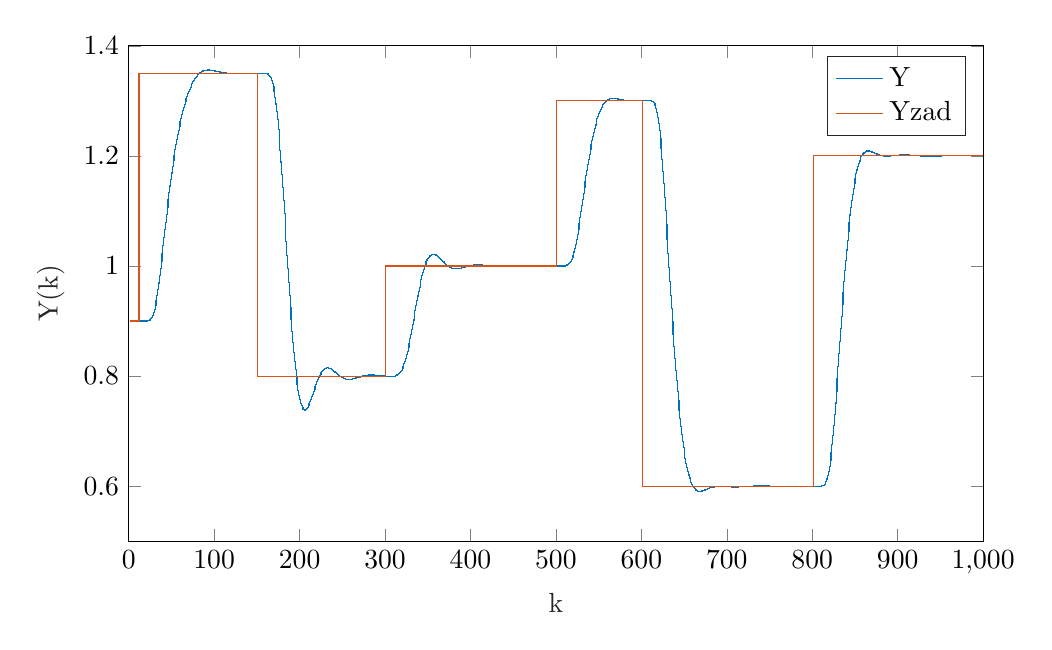
\begin{tikzpicture}

\begin{axis}[%
width=4.272in,
height=2.477in,
at={(0.717in,0.437in)},
scale only axis,
xmin=0,
xmax=1000,
xlabel style={font=\color{white!15!black}},
xlabel={k},
ymin=0.5,
ymax=1.4,
ylabel style={font=\color{white!15!black}},
ylabel={Y(k)},
axis background/.style={fill=white},
legend style={legend cell align=left, align=left, draw=white!15!black}
]
\addplot[const plot, color=mycolor1] table[row sep=crcr] {%
1	0.9\\
2	0.9\\
3	0.9\\
4	0.9\\
5	0.9\\
6	0.9\\
7	0.9\\
8	0.9\\
9	0.9\\
10	0.9\\
11	0.9\\
12	0.9\\
13	0.9\\
14	0.9\\
15	0.9\\
16	0.9\\
17	0.9\\
18	0.9\\
19	0.9\\
20	0.9\\
21	0.9\\
22	0.9003968325\\
23	0.90110505465075\\
24	0.901855517129444\\
25	0.902945719845552\\
26	0.904625024635009\\
27	0.907100496676831\\
28	0.91054211410946\\
29	0.915087410118447\\
30	0.920845605469288\\
31	0.92790128376342\\
32	0.936299298339035\\
33	0.946052635636149\\
34	0.957058874920676\\
35	0.969087763436251\\
36	0.981904316990178\\
37	0.995304815391286\\
38	1.00911327597092\\
39	1.02317829442478\\
40	1.03737021644321\\
41	1.05157860712455\\
42	1.06570998836003\\
43	1.07968581726912\\
44	1.09344068138123\\
45	1.10692068862719\\
46	1.12008203234643\\
47	1.13288971345403\\
48	1.1453164036644\\
49	1.15734143525381\\
50	1.16894990427704\\
51	1.1801318754488\\
52	1.19088167807166\\
53	1.20119728344962\\
54	1.21107975518261\\
55	1.22053276459969\\
56	1.22956216436839\\
57	1.23817561402087\\
58	1.24638225177231\\
59	1.2541924075798\\
60	1.26161735290653\\
61	1.26866908312168\\
62	1.2753601288866\\
63	1.28170339325598\\
64	1.28771176326501\\
65	1.29339744332356\\
66	1.29877167457601\\
67	1.30384485966085\\
68	1.30862667317233\\
69	1.31312615908228\\
70	1.31735181631137\\
71	1.32131167356728\\
72	1.32501335449577\\
73	1.32846413411848\\
74	1.33167099894793\\
75	1.3346407362699\\
76	1.33738004936926\\
77	1.33989566530942\\
78	1.34219442026245\\
79	1.3442833254658\\
80	1.34616961653649\\
81	1.34786078856231\\
82	1.34936461910956\\
83	1.35068918103448\\
84	1.35184284622823\\
85	1.35283427957938\\
86	1.35367242136348\\
87	1.35436645785762\\
88	1.35492578204219\\
89	1.35535994668373\\
90	1.35567861176104\\
91	1.35589148790545\\
92	1.35600827727144\\
93	1.35603861303068\\
94	1.35599199851265\\
95	1.35587774696919\\
96	1.35570492303007\\
97	1.35548228698344\\
98	1.35521824292134\\
99	1.35492079158923\\
100	1.35459748857745\\
101	1.3542554083215\\
102	1.35390111423324\\
103	1.35354063516377\\
104	1.35317944829535\\
105	1.35282246846694\\
106	1.35247404384341\\
107	1.35213795773748\\
108	1.35181743629345\\
109	1.35151516165612\\
110	1.3512332901797\\
111	1.35097347518025\\
112	1.35073689369736\\
113	1.35052427670486\\
114	1.35033594219434\\
115	1.35017183054746\\
116	1.35003154161415\\
117	1.34991437292277\\
118	1.34981935846682\\
119	1.34974530753931\\
120	1.34969084311932\\
121	1.34965443935418\\
122	1.34963445772379\\
123	1.34962918151944\\
124	1.34963684831768\\
125	1.34965568017913\\
126	1.34968391135209\\
127	1.34971981331082\\
128	1.34976171700697\\
129	1.34980803226027\\
130	1.3498572642595\\
131	1.34990802718669\\
132	1.34995905501654\\
133	1.35000920957827\\
134	1.35005748599832\\
135	1.35010301566981\\
136	1.35014506691791\\
137	1.35018304354921\\
138	1.35021648148825\\
139	1.35024504371499\\
140	1.35026851372427\\
141	1.35028678773096\\
142	1.35029986584488\\
143	1.35030784243538\\
144	1.35031089589958\\
145	1.35030927803898\\
146	1.3503033032379\\
147	1.3502933376241\\
148	1.35027978837706\\
149	1.35026309333347\\
150	1.35024371102242\\
151	1.35022211124549\\
152	1.35019876629895\\
153	1.35017414291764\\
154	1.35014869500257\\
155	1.35012285717728\\
156	1.35009703920177\\
157	1.3500716212573\\
158	1.35004695010134\\
159	1.35002333607844\\
160	1.35000105096129\\
161	1.34958334072988\\
162	1.34885556440986\\
163	1.34805167170422\\
164	1.34681140563093\\
165	1.34483295327382\\
166	1.34186584408902\\
167	1.33770461730889\\
168	1.33218318015732\\
169	1.32516978625615\\
170	1.31656257053616\\
171	1.30630394853774\\
172	1.29437214415411\\
173	1.28075011845817\\
174	1.26544384629002\\
175	1.24850317221384\\
176	1.23001472025092\\
177	1.21009570422224\\
178	1.18888853261625\\
179	1.16655611399256\\
180	1.1432777796752\\
181	1.11924490041571\\
182	1.09465640784145\\
183	1.06971624635108\\
184	1.04463144127777\\
185	1.019608491082\\
186	0.994849253404496\\
187	0.970547493626471\\
188	0.9468860074236\\
189	0.924034240145039\\
190	0.902146335767616\\
191	0.881359596148123\\
192	0.861793363233906\\
193	0.843548235051121\\
194	0.82670549952565\\
195	0.811326834548353\\
196	0.797454369296904\\
197	0.785111097002974\\
198	0.774301582885051\\
199	0.765012918912566\\
200	0.757215883907191\\
201	0.750866271554858\\
202	0.745906349301416\\
203	0.742266414746959\\
204	0.739866425425958\\
205	0.738617680646341\\
206	0.738424527472444\\
207	0.739186059146478\\
208	0.740797777167462\\
209	0.743153192809605\\
210	0.746145347742078\\
211	0.749668236795767\\
212	0.753618119108728\\
213	0.757894706886748\\
214	0.762402223441049\\
215	0.767050324069263\\
216	0.771754875448329\\
217	0.776438591790196\\
218	0.781031528640741\\
219	0.785471437510793\\
220	0.789703986476832\\
221	0.793682853531133\\
222	0.797369700827598\\
223	0.800734039076634\\
224	0.803752992223755\\
225	0.80641097325029\\
226	0.808699282472612\\
227	0.810615640056082\\
228	0.812163664576597\\
229	0.813352309367132\\
230	0.814195268107921\\
231	0.814710360684843\\
232	0.814918909775465\\
233	0.814845117948185\\
234	0.814515454297106\\
235	0.813958058800019\\
236	0.813202171693151\\
237	0.812277594219171\\
238	0.811214186142138\\
239	0.810041404453174\\
240	0.808787886730462\\
241	0.807481081681271\\
242	0.80614692849434\\
243	0.804809585778536\\
244	0.803491210066927\\
245	0.80221178313136\\
246	0.80098898668737\\
247	0.799838122477483\\
248	0.798772075206142\\
249	0.797801315363455\\
250	0.796933938618148\\
251	0.796175738181507\\
252	0.795530306341652\\
253	0.794999161238101\\
254	0.794581894886407\\
255	0.794276338467039\\
256	0.794078740956545\\
257	0.793983957296594\\
258	0.793985642461911\\
259	0.79407644799482\\
260	0.794248217815956\\
261	0.79449218039096\\
262	0.794799134625507\\
263	0.795159627169491\\
264	0.795564119129764\\
265	0.79600314051384\\
266	0.796467431049267\\
267	0.796948066340082\\
268	0.797436568628572\\
269	0.797925001723676\\
270	0.798406049933398\\
271	0.798873081094773\\
272	0.799320194029022\\
273	0.799742250959673\\
274	0.800134895616513\\
275	0.800494557907356\\
276	0.800818446172505\\
277	0.801104528143608\\
278	0.801351501809697\\
279	0.801558757449577\\
280	0.801726332122392\\
281	0.801854857918622\\
282	0.801945505263599\\
283	0.801999922536651\\
284	0.802020173223165\\
285	0.802008671756234\\
286	0.801968119131307\\
287	0.801901439293358\\
288	0.801811717203903\\
289	0.801702139396508\\
290	0.801575937726543\\
291	0.801436336915501\\
292	0.801286506384228\\
293	0.801129516764395\\
294	0.800968301375089\\
295	0.800805622852846\\
296	0.800644045029929\\
297	0.800485910068264\\
298	0.800333320775922\\
299	0.800188127960133\\
300	0.800051922605992\\
301	0.799926032613574\\
302	0.79981152377838\\
303	0.799709204660822\\
304	0.799619634959778\\
305	0.799543136982948\\
306	0.799479809792287\\
307	0.799429545596056\\
308	0.799392047959223\\
309	0.799366851410674\\
310	0.799353342038308\\
311	0.799747145802207\\
312	0.800461219978727\\
313	0.801137131115523\\
314	0.801914235020286\\
315	0.802909564461967\\
316	0.804220534911914\\
317	0.805927359437732\\
318	0.808095201985453\\
319	0.810776095441594\\
320	0.814010648296926\\
321	0.817811224735484\\
322	0.822168290482718\\
323	0.827085252389018\\
324	0.832568296429694\\
325	0.838606560823127\\
326	0.845174857465055\\
327	0.852236048423984\\
328	0.859743117931684\\
329	0.867640975725555\\
330	0.875868023532365\\
331	0.884358361157965\\
332	0.893044379041932\\
333	0.90185741400619\\
334	0.91072731326583\\
335	0.919583327841148\\
336	0.928355716671725\\
337	0.936977094756501\\
338	0.945383559489385\\
339	0.95351562499849\\
340	0.961318990480656\\
341	0.968745125941273\\
342	0.975751631618355\\
343	0.982302445482036\\
344	0.988368035205403\\
345	0.993925561612596\\
346	0.998958923245054\\
347	1.00345866344708\\
348	1.00742176188568\\
349	1.010851329325\\
350	1.01375622180978\\
351	1.01615058993168\\
352	1.01805338152754\\
353	1.01948781458492\\
354	1.020480827554\\
355	1.02106250891741\\
356	1.02126551264829\\
357	1.02112447102456\\
358	1.02067541609307\\
359	1.01995521928491\\
360	1.01900105715883\\
361	1.01784990987019\\
362	1.0165380974831\\
363	1.01510085771875\\
364	1.01357196771876\\
365	1.01198341204929\\
366	1.01036509882584\\
367	1.00874462505388\\
368	1.00714709128741\\
369	1.0055949647985\\
370	1.004107989686\\
371	1.00270314170915\\
372	1.00139462511279\\
373	1.00019390831965\\
374	0.999109795081515\\
375	0.998148527452401\\
376	0.99731391674406\\
377	0.996607498468375\\
378	0.996028707191567\\
379	0.995575067227566\\
380	0.995242395172641\\
381	0.995025010419041\\
382	0.994915949971621\\
383	0.994907184117542\\
384	0.994989829755187\\
385	0.995154358467745\\
386	0.995390796726505\\
387	0.995688915925825\\
388	0.996038410280957\\
389	0.996429060954596\\
390	0.996850885111547\\
391	0.997294268927672\\
392	0.997750083894303\\
393	0.998209786058853\\
394	0.998665498123301\\
395	0.999110074582204\\
396	0.999537150318976\\
397	0.999941173291637\\
398	1.00031742212554\\
399	1.00066200958994\\
400	1.00097187306723\\
401	1.00124475322839\\
402	1.00147916220643\\
403	1.00167434261212\\
404	1.00183021876461\\
405	1.00194734151501\\
406	1.00202682802539\\
407	1.00207029783102\\
408	1.00207980646155\\
409	1.00205777783008\\
410	1.00200693651925\\
411	1.00193024100311\\
412	1.00183081874504\\
413	1.00171190400695\\
414	1.0015767790962\\
415	1.0014287196653\\
416	1.00127094456832\\
417	1.0011065706676\\
418	1.0009385728775\\
419	1.00076974962892\\
420	1.0006026938413\\
421	1.00043976939788\\
422	1.00028309303694\\
423	1.00013452149627\\
424	0.99999564368167\\
425	0.999867777572143\\
426	0.999751971526009\\
427	0.999649009612091\\
428	0.999559420559455\\
429	0.999483489896953\\
430	0.999421274839894\\
431	0.999372621475178\\
432	0.999337183797433\\
433	0.999314444156654\\
434	0.999303734691846\\
435	0.999304259344428\\
436	0.999315116069145\\
437	0.999335318887987\\
438	0.999363819463591\\
439	0.999399527901949\\
440	0.999441332529343\\
441	0.999488118424576\\
442	0.999538784524078\\
443	0.999592259153903\\
444	0.99964751387826\\
445	0.999703575588713\\
446	0.99975953679104\\
447	0.999814564077596\\
448	0.999867904801609\\
449	0.999918891995832\\
450	0.99996694760128\\
451	1.00001158409218\\
452	1.00005240460072\\
453	1.00008910165971\\
454	1.0001214546927\\
455	1.00014932638984\\
456	1.00017265811363\\
457	1.00019146448161\\
458	1.00020582727424\\
459	1.00021588881406\\
460	1.00022184495891\\
461	1.0002239378462\\
462	1.0002224485182\\
463	1.00021768954946\\
464	1.00020999778799\\
465	1.00019972731102\\
466	1.00018724268478\\
467	1.00017291260618\\
468	1.00015710399197\\
469	1.00014017656905\\
470	1.00012247800784\\
471	1.00010433962861\\
472	1.0000860727002\\
473	1.00006796533936\\
474	1.00005028000969\\
475	1.00003325160999\\
476	1.00001708613349\\
477	1.00000195987267\\
478	0.9999880191378\\
479	0.999975380452334\\
480	0.999964131183799\\
481	0.999954330565763\\
482	0.999946011063954\\
483	0.9999391800382\\
484	0.99993382165126\\
485	0.999929898975791\\
486	0.999927356251606\\
487	0.999926121246955\\
488	0.999926107679666\\
489	0.999927217656662\\
490	0.999929344093398\\
491	0.999932373078146\\
492	0.999936186149736\\
493	0.999940662461168\\
494	0.999945680805464\\
495	0.999951121484121\\
496	0.999956868002484\\
497	0.999962808580231\\
498	0.999968837468934\\
499	0.999974856072218\\
500	0.999980773867385\\
501	0.999986509130492\\
502	0.999991989469671\\
503	0.999997152174013\\
504	1.00000194438755\\
505	1.00000632311974\\
506	1.00001025510544\\
507	1.00001371652858\\
508	1.0000166926247\\
509	1.00001917717803\\
510	1.00002117192937\\
511	1.0004195449335\\
512	1.00112891366314\\
513	1.00182725017615\\
514	1.00271763732632\\
515	1.00397055816371\\
516	1.00572784155662\\
517	1.00810618151233\\
518	1.0112002735443\\
519	1.01508560718794\\
520	1.01982094992674\\
521	1.02543219488498\\
522	1.0319192837372\\
523	1.03928997308108\\
524	1.04754737834576\\
525	1.0566317132164\\
526	1.06639836538493\\
527	1.07667941025496\\
528	1.08732957546695\\
529	1.09822367087069\\
530	1.10925428704098\\
531	1.1203297355759\\
532	1.13137220700448\\
533	1.14231612447253\\
534	1.15310561649104\\
535	1.16368703005368\\
536	1.17400793092584\\
537	1.1840229426173\\
538	1.19369465856563\\
539	1.20299257353384\\
540	1.21189215466165\\
541	1.22037403401715\\
542	1.22842330680877\\
543	1.23602892144447\\
544	1.24318319829968\\
545	1.24988174967445\\
546	1.25612372197485\\
547	1.26191176446338\\
548	1.26725165837002\\
549	1.27215191781551\\
550	1.27662344600476\\
551	1.28067923789546\\
552	1.2843341219404\\
553	1.28760453468895\\
554	1.29050832077801\\
555	1.29306453646901\\
556	1.29529322647289\\
557	1.2972151746531\\
558	1.29885165810183\\
559	1.30022422235566\\
560	1.30135447788016\\
561	1.3022639146056\\
562	1.30297373192754\\
563	1.30350468210268\\
564	1.30387692549464\\
565	1.30410989737243\\
566	1.30422218823278\\
567	1.30423144083229\\
568	1.30415426565023\\
569	1.30400617432765\\
570	1.30380152978975\\
571	1.30355351185071\\
572	1.30327409731068\\
573	1.30297405371648\\
574	1.30266294607418\\
575	1.30234915584046\\
576	1.3020399114018\\
577	1.30174132897958\\
578	1.30145846264576\\
579	1.30119536204714\\
580	1.30095513648506\\
581	1.30074002408007\\
582	1.30055146482137\\
583	1.30039017635624\\
584	1.30025623141862\\
585	1.30014913583531\\
586	1.3000679060926\\
587	1.3000111455096\\
588	1.29997711815368\\
589	1.29996381973837\\
590	1.29996904485279\\
591	1.29999044997537\\
592	1.30002561182321\\
593	1.3000720806832\\
594	1.30012742846191\\
595	1.30018929128112\\
596	1.30025540653226\\
597	1.30032364438645\\
598	1.30039203383484\\
599	1.30045878340358\\
600	1.30052229675018\\
601	1.3005811834008\\
602	1.30063426493354\\
603	1.30068057695002\\
604	1.30071936720783\\
605	1.30075009030848\\
606	1.30077239935129\\
607	1.30078613497146\\
608	1.30079131218211\\
609	1.30078810543522\\
610	1.30077683230584\\
611	1.30036152195789\\
612	1.29962884862786\\
613	1.29876057096594\\
614	1.2973023078033\\
615	1.29487378300001\\
616	1.29115980597449\\
617	1.28590222758991\\
618	1.27889277240375\\
619	1.26996665797662\\
620	1.25899692069623\\
621	1.24590771434788\\
622	1.230664841921\\
623	1.21324630448703\\
624	1.19366412017989\\
625	1.17215752212353\\
626	1.14914359532529\\
627	1.12500251120729\\
628	1.10006291851379\\
629	1.07460780021296\\
630	1.04887971776824\\
631	1.02308550386751\\
632	0.997400458789689\\
633	0.971972100240139\\
634	0.946930173750666\\
635	0.922399309758119\\
636	0.898493979912116\\
637	0.875309896829736\\
638	0.852925734089754\\
639	0.831405424653869\\
640	0.81080015613216\\
641	0.79115010269698\\
642	0.772485928333495\\
643	0.754830091635659\\
644	0.738197670235742\\
645	0.72259629740072\\
646	0.708025903124205\\
647	0.694479186860302\\
648	0.681942488306603\\
649	0.670396568455216\\
650	0.659817281692202\\
651	0.650176156925238\\
652	0.64144090278151\\
653	0.633575849426883\\
654	0.626542351707998\\
655	0.620299209919097\\
656	0.614803150695411\\
657	0.610009337820786\\
658	0.605871858150761\\
659	0.602344165482766\\
660	0.599379487765469\\
661	0.596931203319444\\
662	0.594953190520359\\
663	0.593400154409876\\
664	0.592227932249242\\
665	0.591393776574902\\
666	0.59085661010371\\
667	0.590577246575475\\
668	0.590518575656047\\
669	0.590645713369732\\
670	0.590926120169087\\
671	0.591329688380825\\
672	0.591828800434456\\
673	0.592398359040108\\
674	0.593015790344373\\
675	0.593661021171309\\
676	0.594316431872443\\
677	0.594966786915432\\
678	0.595599145765096\\
679	0.59620275669816\\
680	0.596768936100608\\
681	0.597290935689438\\
682	0.597763800021212\\
683	0.598184216592174\\
684	0.598550360790155\\
685	0.59886173791258\\
686	0.599119024392691\\
687	0.599323910254205\\
688	0.599478944643304\\
689	0.599587386089738\\
690	0.599653058948922\\
691	0.599680217282857\\
692	0.599673417248767\\
693	0.599637398878423\\
694	0.599576977946707\\
695	0.599496948444541\\
696	0.599401995990444\\
697	0.599296622339942\\
698	0.599185080987752\\
699	0.599071323707205\\
700	0.598958957736508\\
701	0.598851213201846\\
702	0.598750920262889\\
703	0.598660495376697\\
704	0.598581936001287\\
705	0.598516823000331\\
706	0.598466329965664\\
707	0.59843123864414\\
708	0.598411959639575\\
709	0.598408557557833\\
710	0.598420779772675\\
711	0.598448088010377\\
712	0.598489691981271\\
713	0.598544584324993\\
714	0.598611576182222\\
715	0.598689332757769\\
716	0.598776408296916\\
717	0.5988712799576\\
718	0.598972380124216\\
719	0.599078126773362\\
720	0.59918695156663\\
721	0.599297325409667\\
722	0.59940778127923\\
723	0.59951693418015\\
724	0.599623498151176\\
725	0.599726300292185\\
726	0.599824291834519\\
727	0.599916556321012\\
728	0.600002315002228\\
729	0.600080929590319\\
730	0.600151902541749\\
731	0.600214875064709\\
732	0.600269623066619\\
733	0.600316051271672\\
734	0.600354185748149\\
735	0.600384165090534\\
736	0.600406230502452\\
737	0.600420715023623\\
738	0.600428032137604\\
739	0.600428663987576\\
740	0.60042314941516\\
741	0.60041207202264\\
742	0.600396048442511\\
743	0.60037571698022\\
744	0.600351726776946\\
745	0.600324727619391\\
746	0.600295360503436\\
747	0.60026424903832\\
748	0.600231991758126\\
749	0.600199155388049\\
750	0.600166269094442\\
751	0.6001338197302\\
752	0.600102248070824\\
753	0.600071946021681\\
754	0.600043254763602\\
755	0.600016463792206\\
756	0.599991810796184\\
757	0.599969482311266\\
758	0.599949615079771\\
759	0.599932298040384\\
760	0.599917574869152\\
761	0.59990544699055\\
762	0.599895876976692\\
763	0.599888792253334\\
764	0.599884089033087\\
765	0.599881636399062\\
766	0.599881280465976\\
767	0.599882848550301\\
768	0.599886153286335\\
769	0.599890996630841\\
770	0.599897173705152\\
771	0.599904476430101\\
772	0.59991269691582\\
773	0.599921630575136\\
774	0.599931078935954\\
775	0.599940852134492\\
776	0.599950771077494\\
777	0.599960669267467\\
778	0.599970394290548\\
779	0.599979808971713\\
780	0.599988792206676\\
781	0.599997239483959\\
782	0.600005063114185\\
783	0.600012192186725\\
784	0.600018572276299\\
785	0.600024164924109\\
786	0.600028946919503\\
787	0.600032909409113\\
788	0.60003605686081\\
789	0.600038405909872\\
790	0.600039984114284\\
791	0.600040828645342\\
792	0.600040984938581\\
793	0.600040505328638\\
794	0.600039447690022\\
795	0.600037874103887\\
796	0.600035849568898\\
797	0.600033440772165\\
798	0.600030714934022\\
799	0.600027738738192\\
800	0.600024577356672\\
801	0.600021293576482\\
802	0.600017947033287\\
803	0.60001459355491\\
804	0.600011284615827\\
805	0.600008066901952\\
806	0.600004981983444\\
807	0.600002066091774\\
808	0.599999349996034\\
809	0.599996858972361\\
810	0.599994612859437\\
811	0.600389439396398\\
812	0.601095871468999\\
813	0.60189766645611\\
814	0.60318676439121\\
815	0.605291429440016\\
816	0.608483986657748\\
817	0.612987721490138\\
818	0.618983027215646\\
819	0.626612877175766\\
820	0.635987691088123\\
821	0.647171300595027\\
822	0.660189752412603\\
823	0.675061840521229\\
824	0.691779649625122\\
825	0.710232613358692\\
826	0.730137395469929\\
827	0.751142299413972\\
828	0.772942924982412\\
829	0.79527680918064\\
830	0.817918626691486\\
831	0.84067589418608\\
832	0.863385128129969\\
833	0.885908410609495\\
834	0.908125182727549\\
835	0.929916810629886\\
836	0.951167015543122\\
837	0.97177461992197\\
838	0.991656163186357\\
839	1.01074353554539\\
840	1.02898191836234\\
841	1.04632799161604\\
842	1.06274837399523\\
843	1.07821826553208\\
844	1.09272050427021\\
845	1.10624558831043\\
846	1.11879225336267\\
847	1.13036735100295\\
848	1.1409849674405\\
849	1.15066546463136\\
850	1.15943465354276\\
851	1.16732307918269\\
852	1.17436540015301\\
853	1.18059984816852\\
854	1.18606774427222\\
855	1.19081301346489\\
856	1.19488163405928\\
857	1.19832103373595\\
858	1.20117950152222\\
859	1.20350565558333\\
860	1.20534796690914\\
861	1.20675433057128\\
862	1.20777167775477\\
863	1.20844562302977\\
864	1.20882014287491\\
865	1.20893728501145\\
866	1.20883691343985\\
867	1.20855649614552\\
868	1.20813093857259\\
869	1.20759246097209\\
870	1.20697051587709\\
871	1.20629174224063\\
872	1.20557995335243\\
873	1.20485615610839\\
874	1.20413859954053\\
875	1.20344285062163\\
876	1.20278189506791\\
877	1.20216626024792\\
878	1.20160415678389\\
879	1.2011016353136\\
880	1.20066275506962\\
881	1.2002897611921\\
882	1.19998326791433\\
883	1.19974244493938\\
884	1.19956520447423\\
885	1.19944838651865\\
886	1.1993879401508\\
887	1.19937909873954\\
888	1.19941654725757\\
889	1.19949458014402\\
890	1.19960724844059\\
891	1.19974849518375\\
892	1.19991227827571\\
893	1.20009268028315\\
894	1.20028400482713\\
895	1.20048085943364\\
896	1.20067822491068\\
897	1.20087151150244\\
898	1.20105660223947\\
899	1.2012298840514\\
900	1.20138826733411\\
901	1.20152919476761\\
902	1.20165064026437\\
903	1.20175109899304\\
904	1.20182956946918\\
905	1.20188552873414\\
906	1.20191890165592\\
907	1.20193002538274\\
908	1.20191960996135\\
909	1.20188869610062\\
910	1.20183861101696\\
911	1.20177092324467\\
912	1.20168739723201\\
913	1.20158994847486\\
914	1.20148059986602\\
915	1.20136143985971\\
916	1.20123458297094\\
917	1.20110213304764\\
918	1.20096614967255\\
919	1.20082861797204\\
920	1.20069142203201\\
921	1.20055632204741\\
922	1.20042493526261\\
923	1.2002987206957\\
924	1.20017896758072\\
925	1.20006678740942\\
926	1.19996310940706\\
927	1.1998686792372\\
928	1.19978406069626\\
929	1.1997096401319\\
930	1.19964563329837\\
931	1.19959209434724\\
932	1.19954892664343\\
933	1.199515895093\\
934	1.19949263967116\\
935	1.19947868984532\\
936	1.19947347959909\\
937	1.19947636277685\\
938	1.19948662848682\\
939	1.19950351632001\\
940	1.19952623116513\\
941	1.19955395742317\\
942	1.19958587245026\\
943	1.19962115908313\\
944	1.19965901712704\\
945	1.1996986737116\\
946	1.19973939244492\\
947	1.19978048132019\\
948	1.19982129935201\\
949	1.19986126194045\\
950	1.19989984498102\\
951	1.19993658775599\\
952	1.1999710946586\\
953	1.20000303581522\\
954	1.20003214668233\\
955	1.20005822670454\\
956	1.20008113712754\\
957	1.20010079806506\\
958	1.20011718492264\\
959	1.20013032428248\\
960	1.20014028935362\\
961	1.20014719509003\\
962	1.20015119307617\\
963	1.20015246627504\\
964	1.20015122372861\\
965	1.20014769529365\\
966	1.20014212648937\\
967	1.20013477352522\\
968	1.20012589856904\\
969	1.20011576530756\\
970	1.20010463484253\\
971	1.2000927619572\\
972	1.20008039177985\\
973	1.20006775686246\\
974	1.20005507468537\\
975	1.20004254559115\\
976	1.20003035114451\\
977	1.2000186529084\\
978	1.20000759162159\\
979	1.19999728675764\\
980	1.19998783644123\\
981	1.19997931769432\\
982	1.19997178698194\\
983	1.19996528102505\\
984	1.19995981784681\\
985	1.19995539801752\\
986	1.1999520060634\\
987	1.19994961200473\\
988	1.19994817298951\\
989	1.19994763499044\\
990	1.19994793453409\\
991	1.19994900043372\\
992	1.19995075549919\\
993	1.19995311819968\\
994	1.19995600425809\\
995	1.1999593281583\\
996	1.1999630045495\\
997	1.19996694953455\\
998	1.19997108183234\\
999	1.1999753238064\\
1000	1.19997960235522\\
};
\addlegendentry{Y}

\addplot[const plot, color=mycolor2] table[row sep=crcr] {%
1	0.9\\
2	0.9\\
3	0.9\\
4	0.9\\
5	0.9\\
6	0.9\\
7	0.9\\
8	0.9\\
9	0.9\\
10	0.9\\
11	0.9\\
12	1.35\\
13	1.35\\
14	1.35\\
15	1.35\\
16	1.35\\
17	1.35\\
18	1.35\\
19	1.35\\
20	1.35\\
21	1.35\\
22	1.35\\
23	1.35\\
24	1.35\\
25	1.35\\
26	1.35\\
27	1.35\\
28	1.35\\
29	1.35\\
30	1.35\\
31	1.35\\
32	1.35\\
33	1.35\\
34	1.35\\
35	1.35\\
36	1.35\\
37	1.35\\
38	1.35\\
39	1.35\\
40	1.35\\
41	1.35\\
42	1.35\\
43	1.35\\
44	1.35\\
45	1.35\\
46	1.35\\
47	1.35\\
48	1.35\\
49	1.35\\
50	1.35\\
51	1.35\\
52	1.35\\
53	1.35\\
54	1.35\\
55	1.35\\
56	1.35\\
57	1.35\\
58	1.35\\
59	1.35\\
60	1.35\\
61	1.35\\
62	1.35\\
63	1.35\\
64	1.35\\
65	1.35\\
66	1.35\\
67	1.35\\
68	1.35\\
69	1.35\\
70	1.35\\
71	1.35\\
72	1.35\\
73	1.35\\
74	1.35\\
75	1.35\\
76	1.35\\
77	1.35\\
78	1.35\\
79	1.35\\
80	1.35\\
81	1.35\\
82	1.35\\
83	1.35\\
84	1.35\\
85	1.35\\
86	1.35\\
87	1.35\\
88	1.35\\
89	1.35\\
90	1.35\\
91	1.35\\
92	1.35\\
93	1.35\\
94	1.35\\
95	1.35\\
96	1.35\\
97	1.35\\
98	1.35\\
99	1.35\\
100	1.35\\
101	1.35\\
102	1.35\\
103	1.35\\
104	1.35\\
105	1.35\\
106	1.35\\
107	1.35\\
108	1.35\\
109	1.35\\
110	1.35\\
111	1.35\\
112	1.35\\
113	1.35\\
114	1.35\\
115	1.35\\
116	1.35\\
117	1.35\\
118	1.35\\
119	1.35\\
120	1.35\\
121	1.35\\
122	1.35\\
123	1.35\\
124	1.35\\
125	1.35\\
126	1.35\\
127	1.35\\
128	1.35\\
129	1.35\\
130	1.35\\
131	1.35\\
132	1.35\\
133	1.35\\
134	1.35\\
135	1.35\\
136	1.35\\
137	1.35\\
138	1.35\\
139	1.35\\
140	1.35\\
141	1.35\\
142	1.35\\
143	1.35\\
144	1.35\\
145	1.35\\
146	1.35\\
147	1.35\\
148	1.35\\
149	1.35\\
150	1.35\\
151	0.8\\
152	0.8\\
153	0.8\\
154	0.8\\
155	0.8\\
156	0.8\\
157	0.8\\
158	0.8\\
159	0.8\\
160	0.8\\
161	0.8\\
162	0.8\\
163	0.8\\
164	0.8\\
165	0.8\\
166	0.8\\
167	0.8\\
168	0.8\\
169	0.8\\
170	0.8\\
171	0.8\\
172	0.8\\
173	0.8\\
174	0.8\\
175	0.8\\
176	0.8\\
177	0.8\\
178	0.8\\
179	0.8\\
180	0.8\\
181	0.8\\
182	0.8\\
183	0.8\\
184	0.8\\
185	0.8\\
186	0.8\\
187	0.8\\
188	0.8\\
189	0.8\\
190	0.8\\
191	0.8\\
192	0.8\\
193	0.8\\
194	0.8\\
195	0.8\\
196	0.8\\
197	0.8\\
198	0.8\\
199	0.8\\
200	0.8\\
201	0.8\\
202	0.8\\
203	0.8\\
204	0.8\\
205	0.8\\
206	0.8\\
207	0.8\\
208	0.8\\
209	0.8\\
210	0.8\\
211	0.8\\
212	0.8\\
213	0.8\\
214	0.8\\
215	0.8\\
216	0.8\\
217	0.8\\
218	0.8\\
219	0.8\\
220	0.8\\
221	0.8\\
222	0.8\\
223	0.8\\
224	0.8\\
225	0.8\\
226	0.8\\
227	0.8\\
228	0.8\\
229	0.8\\
230	0.8\\
231	0.8\\
232	0.8\\
233	0.8\\
234	0.8\\
235	0.8\\
236	0.8\\
237	0.8\\
238	0.8\\
239	0.8\\
240	0.8\\
241	0.8\\
242	0.8\\
243	0.8\\
244	0.8\\
245	0.8\\
246	0.8\\
247	0.8\\
248	0.8\\
249	0.8\\
250	0.8\\
251	0.8\\
252	0.8\\
253	0.8\\
254	0.8\\
255	0.8\\
256	0.8\\
257	0.8\\
258	0.8\\
259	0.8\\
260	0.8\\
261	0.8\\
262	0.8\\
263	0.8\\
264	0.8\\
265	0.8\\
266	0.8\\
267	0.8\\
268	0.8\\
269	0.8\\
270	0.8\\
271	0.8\\
272	0.8\\
273	0.8\\
274	0.8\\
275	0.8\\
276	0.8\\
277	0.8\\
278	0.8\\
279	0.8\\
280	0.8\\
281	0.8\\
282	0.8\\
283	0.8\\
284	0.8\\
285	0.8\\
286	0.8\\
287	0.8\\
288	0.8\\
289	0.8\\
290	0.8\\
291	0.8\\
292	0.8\\
293	0.8\\
294	0.8\\
295	0.8\\
296	0.8\\
297	0.8\\
298	0.8\\
299	0.8\\
300	0.8\\
301	1\\
302	1\\
303	1\\
304	1\\
305	1\\
306	1\\
307	1\\
308	1\\
309	1\\
310	1\\
311	1\\
312	1\\
313	1\\
314	1\\
315	1\\
316	1\\
317	1\\
318	1\\
319	1\\
320	1\\
321	1\\
322	1\\
323	1\\
324	1\\
325	1\\
326	1\\
327	1\\
328	1\\
329	1\\
330	1\\
331	1\\
332	1\\
333	1\\
334	1\\
335	1\\
336	1\\
337	1\\
338	1\\
339	1\\
340	1\\
341	1\\
342	1\\
343	1\\
344	1\\
345	1\\
346	1\\
347	1\\
348	1\\
349	1\\
350	1\\
351	1\\
352	1\\
353	1\\
354	1\\
355	1\\
356	1\\
357	1\\
358	1\\
359	1\\
360	1\\
361	1\\
362	1\\
363	1\\
364	1\\
365	1\\
366	1\\
367	1\\
368	1\\
369	1\\
370	1\\
371	1\\
372	1\\
373	1\\
374	1\\
375	1\\
376	1\\
377	1\\
378	1\\
379	1\\
380	1\\
381	1\\
382	1\\
383	1\\
384	1\\
385	1\\
386	1\\
387	1\\
388	1\\
389	1\\
390	1\\
391	1\\
392	1\\
393	1\\
394	1\\
395	1\\
396	1\\
397	1\\
398	1\\
399	1\\
400	1\\
401	1\\
402	1\\
403	1\\
404	1\\
405	1\\
406	1\\
407	1\\
408	1\\
409	1\\
410	1\\
411	1\\
412	1\\
413	1\\
414	1\\
415	1\\
416	1\\
417	1\\
418	1\\
419	1\\
420	1\\
421	1\\
422	1\\
423	1\\
424	1\\
425	1\\
426	1\\
427	1\\
428	1\\
429	1\\
430	1\\
431	1\\
432	1\\
433	1\\
434	1\\
435	1\\
436	1\\
437	1\\
438	1\\
439	1\\
440	1\\
441	1\\
442	1\\
443	1\\
444	1\\
445	1\\
446	1\\
447	1\\
448	1\\
449	1\\
450	1\\
451	1\\
452	1\\
453	1\\
454	1\\
455	1\\
456	1\\
457	1\\
458	1\\
459	1\\
460	1\\
461	1\\
462	1\\
463	1\\
464	1\\
465	1\\
466	1\\
467	1\\
468	1\\
469	1\\
470	1\\
471	1\\
472	1\\
473	1\\
474	1\\
475	1\\
476	1\\
477	1\\
478	1\\
479	1\\
480	1\\
481	1\\
482	1\\
483	1\\
484	1\\
485	1\\
486	1\\
487	1\\
488	1\\
489	1\\
490	1\\
491	1\\
492	1\\
493	1\\
494	1\\
495	1\\
496	1\\
497	1\\
498	1\\
499	1\\
500	1\\
501	1.3\\
502	1.3\\
503	1.3\\
504	1.3\\
505	1.3\\
506	1.3\\
507	1.3\\
508	1.3\\
509	1.3\\
510	1.3\\
511	1.3\\
512	1.3\\
513	1.3\\
514	1.3\\
515	1.3\\
516	1.3\\
517	1.3\\
518	1.3\\
519	1.3\\
520	1.3\\
521	1.3\\
522	1.3\\
523	1.3\\
524	1.3\\
525	1.3\\
526	1.3\\
527	1.3\\
528	1.3\\
529	1.3\\
530	1.3\\
531	1.3\\
532	1.3\\
533	1.3\\
534	1.3\\
535	1.3\\
536	1.3\\
537	1.3\\
538	1.3\\
539	1.3\\
540	1.3\\
541	1.3\\
542	1.3\\
543	1.3\\
544	1.3\\
545	1.3\\
546	1.3\\
547	1.3\\
548	1.3\\
549	1.3\\
550	1.3\\
551	1.3\\
552	1.3\\
553	1.3\\
554	1.3\\
555	1.3\\
556	1.3\\
557	1.3\\
558	1.3\\
559	1.3\\
560	1.3\\
561	1.3\\
562	1.3\\
563	1.3\\
564	1.3\\
565	1.3\\
566	1.3\\
567	1.3\\
568	1.3\\
569	1.3\\
570	1.3\\
571	1.3\\
572	1.3\\
573	1.3\\
574	1.3\\
575	1.3\\
576	1.3\\
577	1.3\\
578	1.3\\
579	1.3\\
580	1.3\\
581	1.3\\
582	1.3\\
583	1.3\\
584	1.3\\
585	1.3\\
586	1.3\\
587	1.3\\
588	1.3\\
589	1.3\\
590	1.3\\
591	1.3\\
592	1.3\\
593	1.3\\
594	1.3\\
595	1.3\\
596	1.3\\
597	1.3\\
598	1.3\\
599	1.3\\
600	1.3\\
601	0.6\\
602	0.6\\
603	0.6\\
604	0.6\\
605	0.6\\
606	0.6\\
607	0.6\\
608	0.6\\
609	0.6\\
610	0.6\\
611	0.6\\
612	0.6\\
613	0.6\\
614	0.6\\
615	0.6\\
616	0.6\\
617	0.6\\
618	0.6\\
619	0.6\\
620	0.6\\
621	0.6\\
622	0.6\\
623	0.6\\
624	0.6\\
625	0.6\\
626	0.6\\
627	0.6\\
628	0.6\\
629	0.6\\
630	0.6\\
631	0.6\\
632	0.6\\
633	0.6\\
634	0.6\\
635	0.6\\
636	0.6\\
637	0.6\\
638	0.6\\
639	0.6\\
640	0.6\\
641	0.6\\
642	0.6\\
643	0.6\\
644	0.6\\
645	0.6\\
646	0.6\\
647	0.6\\
648	0.6\\
649	0.6\\
650	0.6\\
651	0.6\\
652	0.6\\
653	0.6\\
654	0.6\\
655	0.6\\
656	0.6\\
657	0.6\\
658	0.6\\
659	0.6\\
660	0.6\\
661	0.6\\
662	0.6\\
663	0.6\\
664	0.6\\
665	0.6\\
666	0.6\\
667	0.6\\
668	0.6\\
669	0.6\\
670	0.6\\
671	0.6\\
672	0.6\\
673	0.6\\
674	0.6\\
675	0.6\\
676	0.6\\
677	0.6\\
678	0.6\\
679	0.6\\
680	0.6\\
681	0.6\\
682	0.6\\
683	0.6\\
684	0.6\\
685	0.6\\
686	0.6\\
687	0.6\\
688	0.6\\
689	0.6\\
690	0.6\\
691	0.6\\
692	0.6\\
693	0.6\\
694	0.6\\
695	0.6\\
696	0.6\\
697	0.6\\
698	0.6\\
699	0.6\\
700	0.6\\
701	0.6\\
702	0.6\\
703	0.6\\
704	0.6\\
705	0.6\\
706	0.6\\
707	0.6\\
708	0.6\\
709	0.6\\
710	0.6\\
711	0.6\\
712	0.6\\
713	0.6\\
714	0.6\\
715	0.6\\
716	0.6\\
717	0.6\\
718	0.6\\
719	0.6\\
720	0.6\\
721	0.6\\
722	0.6\\
723	0.6\\
724	0.6\\
725	0.6\\
726	0.6\\
727	0.6\\
728	0.6\\
729	0.6\\
730	0.6\\
731	0.6\\
732	0.6\\
733	0.6\\
734	0.6\\
735	0.6\\
736	0.6\\
737	0.6\\
738	0.6\\
739	0.6\\
740	0.6\\
741	0.6\\
742	0.6\\
743	0.6\\
744	0.6\\
745	0.6\\
746	0.6\\
747	0.6\\
748	0.6\\
749	0.6\\
750	0.6\\
751	0.6\\
752	0.6\\
753	0.6\\
754	0.6\\
755	0.6\\
756	0.6\\
757	0.6\\
758	0.6\\
759	0.6\\
760	0.6\\
761	0.6\\
762	0.6\\
763	0.6\\
764	0.6\\
765	0.6\\
766	0.6\\
767	0.6\\
768	0.6\\
769	0.6\\
770	0.6\\
771	0.6\\
772	0.6\\
773	0.6\\
774	0.6\\
775	0.6\\
776	0.6\\
777	0.6\\
778	0.6\\
779	0.6\\
780	0.6\\
781	0.6\\
782	0.6\\
783	0.6\\
784	0.6\\
785	0.6\\
786	0.6\\
787	0.6\\
788	0.6\\
789	0.6\\
790	0.6\\
791	0.6\\
792	0.6\\
793	0.6\\
794	0.6\\
795	0.6\\
796	0.6\\
797	0.6\\
798	0.6\\
799	0.6\\
800	0.6\\
801	1.2\\
802	1.2\\
803	1.2\\
804	1.2\\
805	1.2\\
806	1.2\\
807	1.2\\
808	1.2\\
809	1.2\\
810	1.2\\
811	1.2\\
812	1.2\\
813	1.2\\
814	1.2\\
815	1.2\\
816	1.2\\
817	1.2\\
818	1.2\\
819	1.2\\
820	1.2\\
821	1.2\\
822	1.2\\
823	1.2\\
824	1.2\\
825	1.2\\
826	1.2\\
827	1.2\\
828	1.2\\
829	1.2\\
830	1.2\\
831	1.2\\
832	1.2\\
833	1.2\\
834	1.2\\
835	1.2\\
836	1.2\\
837	1.2\\
838	1.2\\
839	1.2\\
840	1.2\\
841	1.2\\
842	1.2\\
843	1.2\\
844	1.2\\
845	1.2\\
846	1.2\\
847	1.2\\
848	1.2\\
849	1.2\\
850	1.2\\
851	1.2\\
852	1.2\\
853	1.2\\
854	1.2\\
855	1.2\\
856	1.2\\
857	1.2\\
858	1.2\\
859	1.2\\
860	1.2\\
861	1.2\\
862	1.2\\
863	1.2\\
864	1.2\\
865	1.2\\
866	1.2\\
867	1.2\\
868	1.2\\
869	1.2\\
870	1.2\\
871	1.2\\
872	1.2\\
873	1.2\\
874	1.2\\
875	1.2\\
876	1.2\\
877	1.2\\
878	1.2\\
879	1.2\\
880	1.2\\
881	1.2\\
882	1.2\\
883	1.2\\
884	1.2\\
885	1.2\\
886	1.2\\
887	1.2\\
888	1.2\\
889	1.2\\
890	1.2\\
891	1.2\\
892	1.2\\
893	1.2\\
894	1.2\\
895	1.2\\
896	1.2\\
897	1.2\\
898	1.2\\
899	1.2\\
900	1.2\\
901	1.2\\
902	1.2\\
903	1.2\\
904	1.2\\
905	1.2\\
906	1.2\\
907	1.2\\
908	1.2\\
909	1.2\\
910	1.2\\
911	1.2\\
912	1.2\\
913	1.2\\
914	1.2\\
915	1.2\\
916	1.2\\
917	1.2\\
918	1.2\\
919	1.2\\
920	1.2\\
921	1.2\\
922	1.2\\
923	1.2\\
924	1.2\\
925	1.2\\
926	1.2\\
927	1.2\\
928	1.2\\
929	1.2\\
930	1.2\\
931	1.2\\
932	1.2\\
933	1.2\\
934	1.2\\
935	1.2\\
936	1.2\\
937	1.2\\
938	1.2\\
939	1.2\\
940	1.2\\
941	1.2\\
942	1.2\\
943	1.2\\
944	1.2\\
945	1.2\\
946	1.2\\
947	1.2\\
948	1.2\\
949	1.2\\
950	1.2\\
951	1.2\\
952	1.2\\
953	1.2\\
954	1.2\\
955	1.2\\
956	1.2\\
957	1.2\\
958	1.2\\
959	1.2\\
960	1.2\\
961	1.2\\
962	1.2\\
963	1.2\\
964	1.2\\
965	1.2\\
966	1.2\\
967	1.2\\
968	1.2\\
969	1.2\\
970	1.2\\
971	1.2\\
972	1.2\\
973	1.2\\
974	1.2\\
975	1.2\\
976	1.2\\
977	1.2\\
978	1.2\\
979	1.2\\
980	1.2\\
981	1.2\\
982	1.2\\
983	1.2\\
984	1.2\\
985	1.2\\
986	1.2\\
987	1.2\\
988	1.2\\
989	1.2\\
990	1.2\\
991	1.2\\
992	1.2\\
993	1.2\\
994	1.2\\
995	1.2\\
996	1.2\\
997	1.2\\
998	1.2\\
999	1.2\\
1000	1.2\\
};
\addlegendentry{Yzad}

\end{axis}
\end{tikzpicture}%
\caption{Śledzenie wartości zadanej dla parametrów $K=1,3$, $T_i=9,75$,  $T_d=2,85$}
\end{figure}

\begin{equation}
E = 42,1248
\end{equation}
\begin{equation}
E_{abs} = 97,2766
\end{equation}

\section{Regulator DMC}

Optymalizując w ten sam sposób wskaźnik $E_{abs}$ regulatora DMC można zauważyć że optymalny wskaźnik zawsze będzię w okolicach $~88,7$. Na przykład dla horyzontu predykcji $N=60$ horyzont sterowania i lambda będą odpowiednio $N_u=5$ i $\lambda=35$:

\begin{figure}[H]
\centering
% This file was created by matlab2tikz.
%
%The latest updates can be retrieved from
%  http://www.mathworks.com/matlabcentral/fileexchange/22022-matlab2tikz-matlab2tikz
%where you can also make suggestions and rate matlab2tikz.
%
\definecolor{mycolor1}{rgb}{0.00000,0.44700,0.74100}%
%
\begin{tikzpicture}

\begin{axis}[%
width=4.272in,
height=2.477in,
at={(0.717in,0.437in)},
scale only axis,
xmin=0,
xmax=1000,
xlabel style={font=\color{white!15!black}},
xlabel={k},
ymin=2.5,
ymax=3.4,
ylabel style={font=\color{white!15!black}},
ylabel={U(k)},
axis background/.style={fill=white}
]
\addplot[const plot, color=mycolor1, forget plot] table[row sep=crcr] {%
1	3\\
2	3\\
3	3\\
4	3\\
5	3\\
6	3\\
7	3\\
8	3\\
9	3\\
10	3\\
11	3\\
12	3.075\\
13	3.14604933991986\\
14	3.20257615892773\\
15	3.24710552643331\\
16	3.281748463047\\
17	3.3\\
18	3.3\\
19	3.3\\
20	3.3\\
21	3.3\\
22	3.3\\
23	3.3\\
24	3.29970332890058\\
25	3.29805865291465\\
26	3.29539757388557\\
27	3.29200019696188\\
28	3.28812146043857\\
29	3.28399557163882\\
30	3.2798241632711\\
31	3.27577095779306\\
32	3.27196084709439\\
33	3.26848183650123\\
34	3.26538901935169\\
35	3.2627107065601\\
36	3.26045500493745\\
37	3.25861508997445\\
38	3.25717340820649\\
39	3.25610500376018\\
40	3.25538013004026\\
41	3.25496627958575\\
42	3.25482974193669\\
43	3.25493678010464\\
44	3.25525450026529\\
45	3.25575147603566\\
46	3.25639817770432\\
47	3.25716724766751\\
48	3.25803365577185\\
49	3.25897476201107\\
50	3.25997030885187\\
51	3.26100236119008\\
52	3.2620552084114\\
53	3.26311524012583\\
54	3.2641708047552\\
55	3.26521205819337\\
56	3.266230808154\\
57	3.26722035851289\\
58	3.26817535688798\\
59	3.26909164783994\\
60	3.26996613338377\\
61	3.27079664194792\\
62	3.27158180647838\\
63	3.27232095203932\\
64	3.27301399299435\\
65	3.27366133964683\\
66	3.27426381406448\\
67	3.2748225747014\\
68	3.27533904935255\\
69	3.27581487592432\\
70	3.27625185047509\\
71	3.2766518819667\\
72	3.27701695316796\\
73	3.27734908716165\\
74	3.27765031892395\\
75	3.27792267146882\\
76	3.27816813607653\\
77	3.27838865615543\\
78	3.27858611431639\\
79	3.27876232227145\\
80	3.27891901319895\\
81	3.27905783624846\\
82	3.27918035288862\\
83	3.27928803482907\\
84	3.27938226327503\\
85	3.27946432929823\\
86	3.27953543513165\\
87	3.2795966962175\\
88	3.27964914385822\\
89	3.27969372833885\\
90	3.27973132240611\\
91	3.279762725005\\
92	3.27978866518777\\
93	3.27980980612251\\
94	3.27982674914006\\
95	3.27984003776779\\
96	3.27985016170802\\
97	3.27985756072626\\
98	3.27986262842189\\
99	3.27986571585956\\
100	3.27986713504497\\
101	3.27986716223333\\
102	3.27986604106254\\
103	3.27986398550649\\
104	3.27986118264678\\
105	3.27985779526325\\
106	3.27985396424602\\
107	3.27984981083282\\
108	3.27984543867707\\
109	3.27984093575298\\
110	3.27983637610455\\
111	3.27983182144614\\
112	3.27982732262236\\
113	3.27982292093559\\
114	3.27981864934898\\
115	3.27981453357348\\
116	3.27981059304652\\
117	3.27980684181053\\
118	3.27980328929874\\
119	3.27979994103554\\
120	3.27979679925861\\
121	3.27979386346931\\
122	3.27979113091766\\
123	3.27978859702799\\
124	3.27978625577069\\
125	3.27978409998538\\
126	3.27978212166024\\
127	3.27978031217216\\
128	3.27977866322298\\
129	3.27977716677858\\
130	3.27977581492612\\
131	3.27977459979929\\
132	3.27977351355094\\
133	3.27977254835754\\
134	3.27977169644394\\
135	3.27977095011963\\
136	3.27977030182053\\
137	3.27976974415172\\
138	3.27976926992818\\
139	3.27976887221159\\
140	3.27976854434201\\
141	3.27976827996381\\
142	3.27976807304578\\
143	3.27976791789554\\
144	3.27976780916885\\
145	3.27976774187433\\
146	3.27976771137416\\
147	3.27976771338095\\
148	3.27976774395125\\
149	3.27976779947611\\
150	3.27976787666897\\
151	3.20476787666897\\
152	3.12976787666897\\
153	3.05492400539449\\
154	2.99574062676294\\
155	2.94947419926231\\
156	2.91383160293765\\
157	2.88689708861785\\
158	2.86707123665072\\
159	2.85301990841434\\
160	2.8436315187034\\
161	2.83798124230227\\
162	2.83530100400952\\
163	2.83495429662865\\
164	2.83641503305404\\
165	2.8392497723988\\
166	2.84310277095472\\
167	2.84768340062721\\
168	2.85275555364089\\
169	2.85812871548161\\
170	2.86365044047311\\
171	2.86920000793653\\
172	2.87468307307904\\
173	2.88002715687064\\
174	2.88517784424062\\
175	2.89009558082148\\
176	2.89475297590705\\
177	2.89913253385818\\
178	2.9032247483656\\
179	2.9070265041743\\
180	2.9105397393939\\
181	2.91377032869473\\
182	2.91672715375976\\
183	2.91942133245084\\
184	2.92186558243586\\
185	2.92407369864683\\
186	2.92606012700579\\
187	2.92783961945514\\
188	2.9294269245588\\
189	2.93083661236885\\
190	2.93208290648116\\
191	2.93317954995551\\
192	2.93413970602499\\
193	2.93497588760164\\
194	2.93569991048809\\
195	2.93632286597614\\
196	2.93685510917205\\
197	2.93730625995196\\
198	2.93768521393302\\
199	2.9380001612589\\
200	2.93825861135162\\
201	2.93846742208443\\
202	2.93863283208929\\
203	2.93876049513053\\
204	2.93885551566248\\
205	2.93892248486134\\
206	2.93896551656445\\
207	2.93898828266094\\
208	2.93899404757335\\
209	2.9389857015515\\
210	2.93896579256921\\
211	2.93893655667277\\
212	2.9388999466796\\
213	2.93885765916704\\
214	2.9388111597257\\
215	2.93876170647916\\
216	2.9387103718943\\
217	2.93865806292374\\
218	2.93860553953572\\
219	2.93855343169659\\
220	2.93850225487874\\
221	2.93845242417177\\
222	2.93840426707756\\
223	2.93835803507173\\
224	2.93831391401371\\
225	2.93827203348719\\
226	2.93823247515044\\
227	2.93819528017396\\
228	2.9381604558399\\
229	2.93812798137406\\
230	2.9380978130783\\
231	2.93806988882679\\
232	2.93804413198618\\
233	2.93802045481567\\
234	2.9379987613992\\
235	2.93797895015809\\
236	2.93796091598899\\
237	2.93794455206832\\
238	2.93792975136085\\
239	2.93791640786725\\
240	2.93790441764182\\
241	2.93789367960921\\
242	2.9378840962059\\
243	2.93787557386979\\
244	2.93786802339904\\
245	2.9378613601987\\
246	2.93785550443222\\
247	2.93785038109253\\
248	2.93784592000612\\
249	2.93784205578163\\
250	2.93783872771341\\
251	2.93783587964879\\
252	2.93783345982716\\
253	2.93783142069741\\
254	2.93782971871968\\
255	2.93782831415642\\
256	2.93782717085689\\
257	2.93782625603883\\
258	2.93782554007013\\
259	2.93782499625313\\
260	2.93782460061334\\
261	2.93782433169435\\
262	2.93782417036011\\
263	2.93782409960555\\
264	2.93782410437617\\
265	2.93782417139714\\
266	2.93782428901219\\
267	2.93782444630096\\
268	2.93782463313377\\
269	2.93782484019874\\
270	2.93782505915737\\
271	2.93782528271534\\
272	2.93782550463274\\
273	2.93782571969214\\
274	2.9378259236385\\
275	2.93782611310171\\
276	2.93782628550938\\
277	2.93782643899604\\
278	2.93782657231249\\
279	2.93782668473857\\
280	2.93782677600098\\
281	2.93782684619751\\
282	2.93782689572831\\
283	2.93782692523433\\
284	2.93782693554309\\
285	2.93782692762135\\
286	2.93782690253439\\
287	2.93782686141143\\
288	2.93782680541666\\
289	2.93782673572537\\
290	2.93782665350458\\
291	2.93782655989783\\
292	2.93782645601337\\
293	2.9378263429156\\
294	2.93782622161913\\
295	2.93782609308512\\
296	2.93782595821965\\
297	2.93782581787376\\
298	2.93782567284484\\
299	2.93782552387924\\
300	2.93782537167591\\
301	2.97603077104801\\
302	3.00663929612435\\
303	3.03096034955376\\
304	3.05008883003046\\
305	3.06494007002671\\
306	3.07627899511389\\
307	3.0847444800741\\
308	3.09086970975989\\
309	3.09509921436649\\
310	3.09780313440824\\
311	3.09928917608232\\
312	3.09981263942546\\
313	3.09958483688583\\
314	3.09878016630076\\
315	3.09754205785044\\
316	3.09598797775516\\
317	3.09421364098361\\
318	3.09229655994742\\
319	3.09029903520023\\
320	3.08827067673927\\
321	3.08625053000185\\
322	3.08426886860405\\
323	3.08234870584427\\
324	3.08050706864829\\
325	3.0787560706737\\
326	3.07710381548176\\
327	3.07555518880719\\
328	3.07411245407879\\
329	3.07277578820933\\
330	3.07154372276632\\
331	3.07041352049295\\
332	3.06938148777673\\
333	3.06844323291934\\
334	3.06759387856987\\
335	3.06682823542561\\
336	3.06614094324025\\
337	3.06552658427873\\
338	3.06497977359359\\
339	3.0644952298489\\
340	3.06406782986512\\
341	3.06369264958809\\
342	3.06336499378366\\
343	3.06308041641653\\
344	3.06283473337864\\
345	3.06262402898135\\
346	3.06244465741053\\
347	3.06229324015935\\
348	3.06216666029553\\
349	3.06206205428408\\
350	3.06197680197034\\
351	3.06190851522849\\
352	3.06185502569517\\
353	3.06181437193496\\
354	3.06178478632167\\
355	3.06176468186627\\
356	3.06175263917691\\
357	3.06174739369764\\
358	3.06174782333998\\
359	3.06175293659382\\
360	3.06176186118082\\
361	3.06177383329436\\
362	3.06178818745367\\
363	3.06180434698669\\
364	3.06182181514522\\
365	3.06184016684714\\
366	3.06185904103348\\
367	3.06187813362258\\
368	3.0618971910393\\
369	3.06191600429429\\
370	3.06193440358589\\
371	3.06195225339577\\
372	3.06196944804895\\
373	3.061985907708\\
374	3.06200157477185\\
375	3.06201641064975\\
376	3.06203039288194\\
377	3.06204351257943\\
378	3.06205577215639\\
379	3.06206718333\\
380	3.06207776536379\\
381	3.06208754353212\\
382	3.06209654778447\\
383	3.06210481159002\\
384	3.06211237094409\\
385	3.06211926351945\\
386	3.06212552794689\\
387	3.0621312032106\\
388	3.06213632814519\\
389	3.06214094102227\\
390	3.06214507921569\\
391	3.06214877893542\\
392	3.06215207502112\\
393	3.06215500078739\\
394	3.06215758791324\\
395	3.06215986636947\\
396	3.06216186437814\\
397	3.06216360839881\\
398	3.06216512313729\\
399	3.06216643157259\\
400	3.06216755499887\\
401	3.06216851307897\\
402	3.0621693239072\\
403	3.06217000407881\\
404	3.06217056876436\\
405	3.06217103178718\\
406	3.06217140570255\\
407	3.06217170187737\\
408	3.06217193056941\\
409	3.06217210100522\\
410	3.06217222145606\\
411	3.06217229931142\\
412	3.06217234114965\\
413	3.0621723528054\\
414	3.06217233943371\\
415	3.06217230557056\\
416	3.06217225518983\\
417	3.06217219212926\\
418	3.06217211996621\\
419	3.06217204194239\\
420	3.06217196092455\\
421	3.06217187939133\\
422	3.06217179943851\\
423	3.06217172279678\\
424	3.06217165085766\\
425	3.06217158470415\\
426	3.06217152514367\\
427	3.06217147274159\\
428	3.06217142785391\\
429	3.06217139065841\\
430	3.06217136118364\\
431	3.06217133933535\\
432	3.06217132492042\\
433	3.06217131766796\\
434	3.06217131724793\\
435	3.06217132328719\\
436	3.06217133538329\\
437	3.062171353116\\
438	3.06217137605702\\
439	3.06217140377779\\
440	3.06217143585581\\
441	3.06217147187959\\
442	3.06217151145229\\
443	3.0621715541944\\
444	3.06217159974545\\
445	3.062171647765\\
446	3.06217169793285\\
447	3.06217174994885\\
448	3.06217180353211\\
449	3.06217185841988\\
450	3.06217191436606\\
451	3.06217197113952\\
452	3.06217202852205\\
453	3.06217208630628\\
454	3.06217214429331\\
455	3.06217220229025\\
456	3.06217226010764\\
457	3.06217231755668\\
458	3.0621723744464\\
459	3.06217243058067\\
460	3.06217248575507\\
461	3.06217253975361\\
462	3.06217259234523\\
463	3.0621726432802\\
464	3.06217269228619\\
465	3.06217273906667\\
466	3.06217278330607\\
467	3.06217282468518\\
468	3.06217286290912\\
469	3.06217289773506\\
470	3.06217292898696\\
471	3.06217295656099\\
472	3.0621729804248\\
473	3.06217300061249\\
474	3.0621730172172\\
475	3.06217303038227\\
476	3.06217304029197\\
477	3.06217303036327\\
478	3.06217299191185\\
479	3.06217292176852\\
480	3.06217282048289\\
481	3.06217269098495\\
482	3.06217253760146\\
483	3.06217236534621\\
484	3.06217217941973\\
485	3.0621719848682\\
486	3.062171786362\\
487	3.0621715880631\\
488	3.06217139355738\\
489	3.06217120583347\\
490	3.06217102729388\\
491	3.0621708597879\\
492	3.06217070465798\\
493	3.06217056279372\\
494	3.06217043468916\\
495	3.0621703205001\\
496	3.06217022009951\\
497	3.06217013312933\\
498	3.0621700590481\\
499	3.06216999717371\\
500	3.06216994672118\\
501	3.11947823807149\\
502	3.1653912305941\\
503	3.20187302646888\\
504	3.2305659719844\\
505	3.25284306414311\\
506	3.26985168964506\\
507	3.28255015905406\\
508	3.29173824808299\\
509	3.29808275049507\\
510	3.3\\
511	3.3\\
512	3.3\\
513	3.29965853075402\\
514	3.29845175293392\\
515	3.29659481023615\\
516	3.294263900384\\
517	3.29160259423435\\
518	3.28872715891069\\
519	3.28573104395549\\
520	3.28269082521747\\
521	3.27967075180371\\
522	3.27672270163504\\
523	3.27388573968528\\
524	3.27118767208853\\
525	3.26864724923461\\
526	3.26627599105034\\
527	3.26407969633717\\
528	3.26205968794109\\
529	3.26021383710889\\
530	3.25853740335423\\
531	3.25702372028159\\
532	3.25566475290314\\
533	3.25445154787122\\
534	3.25337459460458\\
535	3.25242411239799\\
536	3.25159027618153\\
537	3.25086339156087\\
538	3.25023402805867\\
539	3.24969311803927\\
540	3.24923202758762\\
541	3.24884260459351\\
542	3.24851720843353\\
543	3.24824872491841\\
544	3.24803056956311\\
545	3.24785668172205\\
546	3.24772151169758\\
547	3.24762000256409\\
548	3.24754756814119\\
549	3.24750006829038\\
550	3.24747378249047\\
551	3.24746538246391\\
552	3.24747190447187\\
553	3.24749072176736\\
554	3.24751951758753\\
555	3.24755625897723\\
556	3.24759917166105\\
557	3.24764671612006\\
558	3.24769756497875\\
559	3.24775058176661\\
560	3.24780480108553\\
561	3.24785941018728\\
562	3.24791373194435\\
563	3.2479672091807\\
564	3.24801939031662\\
565	3.24806991627225\\
566	3.24811850856793\\
567	3.24816495855483\\
568	3.24820911770706\\
569	3.24825088890488\\
570	3.24829021863914\\
571	3.24832709006781\\
572	3.24836151685738\\
573	3.24839353774405\\
574	3.24842321175274\\
575	3.24845061401452\\
576	3.24847583212679\\
577	3.24849896300355\\
578	3.24852011016679\\
579	3.24853938143322\\
580	3.24855688695413\\
581	3.24857273756932\\
582	3.24858704343921\\
583	3.24859991292239\\
584	3.24861145166864\\
585	3.24862176190031\\
586	3.24863094185733\\
587	3.24863908538379\\
588	3.24864628163612\\
589	3.24865261489492\\
590	3.24865816446462\\
591	3.24866300464684\\
592	3.24866720477478\\
593	3.24867082929771\\
594	3.24867393790594\\
595	3.24867658568765\\
596	3.24867882331034\\
597	3.2486806972206\\
598	3.2486822498566\\
599	3.24868351986892\\
600	3.24868454234543\\
601	3.17368454234543\\
602	3.09868454234543\\
603	3.02368454234543\\
604	2.94868454234543\\
605	2.87694124475885\\
606	2.82097164741206\\
607	2.77796768781489\\
608	2.7455838958358\\
609	2.72186255889987\\
610	2.70517113399761\\
611	2.7\\
612	2.7\\
613	2.7\\
614	2.7\\
615	2.70212205576386\\
616	2.70589592922608\\
617	2.7108879537032\\
618	2.7167441809288\\
619	2.72317738822698\\
620	2.72995613211308\\
621	2.73688960961312\\
622	2.74381577824298\\
623	2.7506016957469\\
624	2.75714611631705\\
625	2.76337666378604\\
626	2.76924419809593\\
627	2.77471809107467\\
628	2.77978232957167\\
629	2.78443230887889\\
630	2.78867220184328\\
631	2.79251280782652\\
632	2.79596980131873\\
633	2.7990623130855\\
634	2.80181178765513\\
635	2.80424107009397\\
636	2.80637368266972\\
637	2.8082332584128\\
638	2.80984310395889\\
639	2.81122586856345\\
640	2.81240329996164\\
641	2.81339607092417\\
642	2.81422366302828\\
643	2.81490429640645\\
644	2.815454896121\\
645	2.81589108739826\\
646	2.81622721328881\\
647	2.81647636944108\\
648	2.81665045161673\\
649	2.81676021236736\\
650	2.81681532395507\\
651	2.81682444515581\\
652	2.81679529004963\\
653	2.81673469729065\\
654	2.81664869867379\\
655	2.81654258608456\\
656	2.81642097614121\\
657	2.81628787202309\\
658	2.81614672212992\\
659	2.81600047534036\\
660	2.81585163273824\\
661	2.81570229575535\\
662	2.81555421074352\\
663	2.81540881003888\\
664	2.8152672496197\\
665	2.81513044349207\\
666	2.81499909496156\\
667	2.81487372496199\\
668	2.81475469761983\\
669	2.81464224321483\\
670	2.81453647869838\\
671	2.8144374259549\\
672	2.8143450279859\\
673	2.81425916319018\\
674	2.8141796579056\\
675	2.81410629736998\\
676	2.81403883524933\\
677	2.81397697667451\\
678	2.81392042232551\\
679	2.81386887089834\\
680	2.81382202152183\\
681	2.81377957603301\\
682	2.81374124105212\\
683	2.8137067298217\\
684	2.81367576379323\\
685	2.8136480739571\\
686	2.81362340192219\\
687	2.81360150075733\\
688	2.81358213561149\\
689	2.81356508413246\\
690	2.81355013670471\\
691	2.81353709652776\\
692	2.81352577955617\\
693	2.813516014321\\
694	2.81350764165204\\
695	2.81350051431811\\
696	2.81349449660074\\
697	2.81348946381532\\
698	2.81348530179432\\
699	2.81348190634513\\
700	2.81347918269239\\
701	2.8134770449128\\
702	2.81347541536949\\
703	2.81347422415178\\
704	2.81347340852547\\
705	2.81347291239772\\
706	2.81347268579977\\
707	2.81347268439027\\
708	2.81347286898109\\
709	2.81347320508697\\
710	2.81347366250009\\
711	2.81347421488985\\
712	2.81347483942817\\
713	2.81347551644\\
714	2.81347622907876\\
715	2.81347696302595\\
716	2.81347770621419\\
717	2.81347844784152\\
718	2.81347917833457\\
719	2.81347988929348\\
720	2.81348057342399\\
721	2.81348122449334\\
722	2.81348183739496\\
723	2.8134824081445\\
724	2.81348293382895\\
725	2.8134834125254\\
726	2.81348384320179\\
727	2.81348422560886\\
728	2.81348456016988\\
729	2.8134848478727\\
730	2.81348509016749\\
731	2.81348528887205\\
732	2.81348544608589\\
733	2.81348556411368\\
734	2.81348564539812\\
735	2.81348569246196\\
736	2.81348570785885\\
737	2.8134856941322\\
738	2.81348565378138\\
739	2.81348558923458\\
740	2.81348550282762\\
741	2.81348539678814\\
742	2.81348527322448\\
743	2.81348513411878\\
744	2.81348498132356\\
745	2.81348481656132\\
746	2.8134846414267\\
747	2.81348445739074\\
748	2.81348426580679\\
749	2.81348406791791\\
750	2.81348386486526\\
751	2.81348365769739\\
752	2.81348344738024\\
753	2.81348323480758\\
754	2.81348302081186\\
755	2.81348280617536\\
756	2.81348259164159\\
757	2.81348237792687\\
758	2.81348216573215\\
759	2.81348195575497\\
760	2.81348174870176\\
761	2.81348154530034\\
762	2.81348134631284\\
763	2.81348115254908\\
764	2.81348096488041\\
765	2.81348078424937\\
766	2.81348061166501\\
767	2.81348044817499\\
768	2.81348029480492\\
769	2.81348015248583\\
770	2.81348002199552\\
771	2.81347990391461\\
772	2.81347979859964\\
773	2.81347970617571\\
774	2.81347962654639\\
775	2.81347955941452\\
776	2.81347950430924\\
777	2.81347949359398\\
778	2.81347955061569\\
779	2.81347969149741\\
780	2.81347992661832\\
781	2.81348026040081\\
782	2.81348068719473\\
783	2.81348119512768\\
784	2.81348176891008\\
785	2.813482391837\\
786	2.81348304717775\\
787	2.81348371910268\\
788	2.81348439326433\\
789	2.81348505712385\\
790	2.81348570009302\\
791	2.81348631354612\\
792	2.81348689074272\\
793	2.81348742669272\\
794	2.81348791798684\\
795	2.81348836260968\\
796	2.81348875974782\\
797	2.81348910960407\\
798	2.813489413225\\
799	2.81348967234139\\
800	2.81348988922015\\
801	2.88848988922015\\
802	2.96348988922015\\
803	3.03848988922015\\
804	3.10719398020407\\
805	3.16108720839603\\
806	3.20278917356733\\
807	3.23448862087622\\
808	3.25801319301199\\
809	3.27488774893526\\
810	3.28638316423516\\
811	3.29355720121774\\
812	3.29728876641055\\
813	3.29830664940601\\
814	3.29721365176606\\
815	3.29450686137854\\
816	3.29059470066171\\
817	3.28581127179042\\
818	3.28042843489178\\
819	3.27466598281444\\
820	3.26870021603889\\
821	3.26267117144097\\
822	3.25668871718957\\
823	3.25083769160279\\
824	3.24518223510409\\
825	3.23976944052205\\
826	3.23463242704538\\
827	3.22979292650113\\
828	3.22526345671155\\
829	3.22104914503857\\
830	3.21714925546429\\
831	3.21355846436248\\
832	3.21026792322968\\
833	3.20726614084652\\
834	3.20453971245108\\
835	3.2020739193778\\
836	3.19985321912242\\
837	3.19786164283463\\
838	3.19608311472836\\
839	3.19450170576513\\
840	3.19310183214821\\
841	3.19186840761639\\
842	3.19078695720255\\
843	3.1898436989921\\
844	3.18902559944783\\
845	3.18832040703899\\
846	3.18771666820101\\
847	3.18720372904245\\
848	3.18677172569186\\
849	3.18641156572754\\
850	3.18611490274695\\
851	3.18587410580086\\
852	3.18568222513299\\
853	3.18553295542139\\
854	3.18542059750946\\
855	3.18534001943493\\
856	3.18528661741305\\
857	3.18525627729985\\
858	3.18524533695082\\
859	3.18525054979668\\
860	3.18526904987898\\
861	3.18529831852178\\
862	3.18533615275999\\
863	3.18538063559929\\
864	3.18543010814395\\
865	3.18548314359835\\
866	3.18553852312258\\
867	3.18559521350271\\
868	3.18565234658057\\
869	3.18570920037605\\
870	3.18576518182609\\
871	3.18581981105841\\
872	3.18587270711396\\
873	3.18592357503003\\
874	3.1859721941953\\
875	3.18601840788868\\
876	3.1860621139154\\
877	3.18610325625607\\
878	3.18614181764763\\
879	3.18617781301809\\
880	3.18621128370128\\
881	3.18624229236127\\
882	3.1862709185604\\
883	3.18629725490925\\
884	3.18632140374053\\
885	3.18634347425346\\
886	3.18636358007876\\
887	3.18638183721868\\
888	3.18639836231984\\
889	3.18641327124037\\
890	3.18642667787632\\
891	3.18643869321526\\
892	3.18644942458818\\
893	3.18645897509353\\
894	3.18646744316981\\
895	3.18647492229568\\
896	3.18648150079864\\
897	3.18648726175549\\
898	3.18649228296971\\
899	3.18649663701249\\
900	3.18650039131583\\
901	3.18650360830767\\
902	3.18650634558\\
903	3.18650865608236\\
904	3.18651058833417\\
905	3.18651218665001\\
906	3.18651349137322\\
907	3.18651453911363\\
908	3.18651536298595\\
909	3.18651599284609\\
910	3.18651645552315\\
911	3.18651677504494\\
912	3.186516972856\\
913	3.18651706802657\\
914	3.18651707745203\\
915	3.186517016042\\
916	3.18651689689894\\
917	3.18651673221725\\
918	3.18651653324413\\
919	3.1865163102686\\
920	3.18651607257058\\
921	3.18651582831958\\
922	3.18651558454605\\
923	3.18651534716392\\
924	3.18651512102764\\
925	3.18651491001132\\
926	3.1865147171004\\
927	3.18651454448928\\
928	3.18651439367962\\
929	3.18651426557598\\
930	3.18651416057641\\
931	3.18651407865644\\
932	3.18651401944567\\
933	3.1865139822965\\
934	3.18651396634508\\
935	3.18651397056451\\
936	3.18651399381089\\
937	3.18651403486248\\
938	3.18651409245266\\
939	3.18651416529724\\
940	3.18651425211662\\
941	3.18651435165344\\
942	3.18651446268623\\
943	3.18651458403959\\
944	3.18651471459127\\
945	3.18651485327666\\
946	3.18651499909114\\
947	3.18651515109036\\
948	3.18651530838904\\
949	3.18651547015844\\
950	3.18651563562259\\
951	3.18651580405368\\
952	3.18651597476668\\
953	3.18651614711317\\
954	3.18651632047476\\
955	3.18651649425595\\
956	3.18651666787656\\
957	3.18651684076382\\
958	3.186517012344\\
959	3.18651718203373\\
960	3.18651734923082\\
961	3.18651751330474\\
962	3.18651767358646\\
963	3.18651782935792\\
964	3.18651797984065\\
965	3.18651812418883\\
966	3.18651826149632\\
967	3.18651839082725\\
968	3.18651851127858\\
969	3.18651862205295\\
970	3.1865187225133\\
971	3.18651881221736\\
972	3.18651889093092\\
973	3.18651895862356\\
974	3.18651901545308\\
975	3.18651906174314\\
976	3.18651909795735\\
977	3.18651909169469\\
978	3.18651901954362\\
979	3.18651886529406\\
980	3.1865186212304\\
981	3.18651828991361\\
982	3.18651788042216\\
983	3.18651740559666\\
984	3.18651688005752\\
985	3.18651631881381\\
986	3.18651573632041\\
987	3.18651514587153\\
988	3.1865145592435\\
989	3.18651398651915\\
990	3.1865134360418\\
991	3.18651291445896\\
992	3.1865124268255\\
993	3.18651197674368\\
994	3.18651156652335\\
995	3.18651119734992\\
996	3.1865108694516\\
997	3.18651058225997\\
998	3.18651033455985\\
999	3.18651012462623\\
1000	3.18650995034699\\
};
\end{axis}
\end{tikzpicture}%
\caption{Sterowanie DMC dla parametrów $N=60$, $N_u=5$,  $\lambda=35$}
\end{figure}

\begin{figure}[H]
\centering
% This file was created by matlab2tikz.
%
%The latest updates can be retrieved from
%  http://www.mathworks.com/matlabcentral/fileexchange/22022-matlab2tikz-matlab2tikz
%where you can also make suggestions and rate matlab2tikz.
%
\definecolor{mycolor1}{rgb}{0.00000,0.44700,0.74100}%
\definecolor{mycolor2}{rgb}{0.85000,0.32500,0.09800}%
%
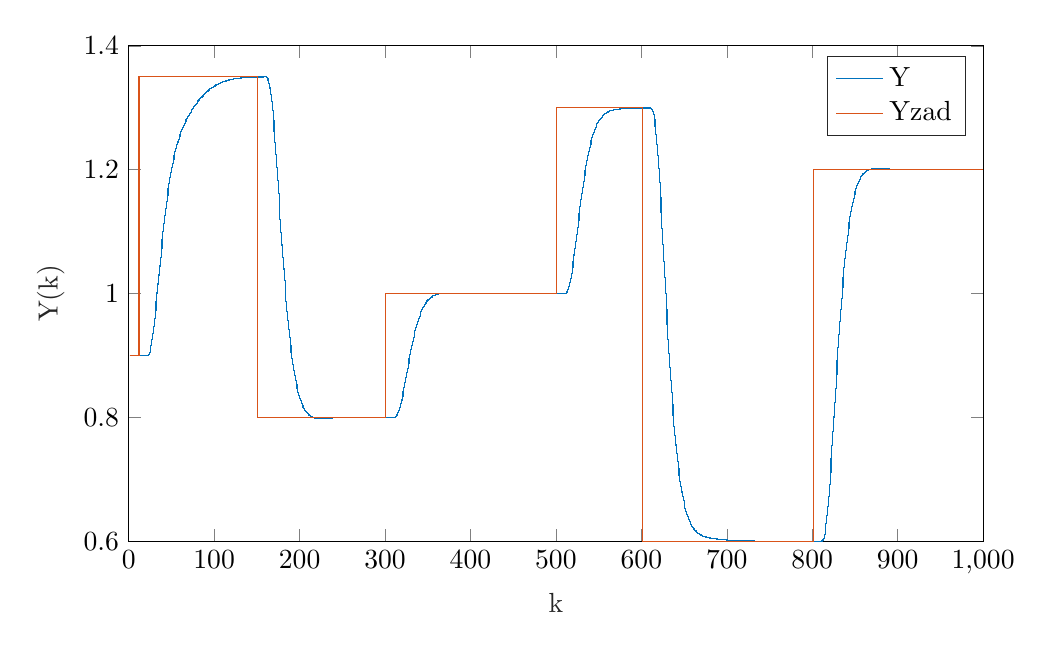
\begin{tikzpicture}

\begin{axis}[%
width=4.272in,
height=2.477in,
at={(0.717in,0.437in)},
scale only axis,
xmin=0,
xmax=1000,
xlabel style={font=\color{white!15!black}},
xlabel={k},
ymin=0.599990102539421,
ymax=1.4,
ylabel style={font=\color{white!15!black}},
ylabel={Y(k)},
axis background/.style={fill=white},
legend style={legend cell align=left, align=left, draw=white!15!black}
]
\addplot[const plot, color=mycolor1] table[row sep=crcr] {%
1	0.9\\
2	0.9\\
3	0.9\\
4	0.9\\
5	0.9\\
6	0.9\\
7	0.9\\
8	0.9\\
9	0.9\\
10	0.9\\
11	0.9\\
12	0.9\\
13	0.9\\
14	0.9\\
15	0.9\\
16	0.9\\
17	0.9\\
18	0.9\\
19	0.9\\
20	0.9\\
21	0.9\\
22	0.9003968325\\
23	0.9018778163132\\
24	0.904920534874846\\
25	0.909782651084776\\
26	0.91655803903601\\
27	0.925177632009263\\
28	0.93539265102329\\
29	0.946891226633101\\
30	0.959401458460744\\
31	0.972686980136867\\
32	0.986542982041154\\
33	1.00079264656616\\
34	1.01528238526758\\
35	1.02987218590751\\
36	1.04443090551421\\
37	1.0588388805302\\
38	1.07298966941558\\
39	1.08679120579388\\
40	1.10016640535896\\
41	1.1130532195654\\
42	1.12540418966581\\
43	1.13718558682714\\
44	1.14837623853603\\
45	1.15896614959036\\
46	1.16895502371311\\
47	1.17835077141539\\
48	1.18716806439894\\
49	1.19542697718571\\
50	1.2031517416538\\
51	1.21036962881352\\
52	1.21710996372025\\
53	1.22340327327814\\
54	1.22928056234493\\
55	1.23477271060248\\
56	1.23990998078933\\
57	1.24472162784209\\
58	1.24923559805658\\
59	1.25347830739522\\
60	1.25747448840416\\
61	1.26124709576398\\
62	1.26481726120054\\
63	1.26820428927123\\
64	1.2714256863681\\
65	1.2744972161122\\
66	1.2774329751263\\
67	1.2802454839502\\
68	1.28294578859206\\
69	1.28554356888324\\
70	1.28804725041939\\
71	1.29046411742628\\
72	1.29280042438433\\
73	1.29506150468481\\
74	1.29725187497446\\
75	1.29937533417848\\
76	1.30143505647785\\
77	1.30343367776004\\
78	1.30537337526624\\
79	1.30725594032775\\
80	1.30908284422244\\
81	1.31085529729334\\
82	1.31257430155888\\
83	1.31424069711058\\
84	1.31585520264339\\
85	1.3174184504971\\
86	1.31893101660893\\
87	1.32039344578718\\
88	1.32180627271829\\
89	1.32317003911366\\
90	1.32448530739215\\
91	1.32575267127851\\
92	1.32697276367974\\
93	1.32814626218008\\
94	1.32927389247323\\
95	1.33035643002664\\
96	1.33139470024904\\
97	1.33238957740889\\
98	1.33334198252772\\
99	1.33425288045007\\
100	1.33512327627015\\
101	1.33595421127443\\
102	1.33674675854051\\
103	1.33750201831417\\
104	1.33822111326995\\
105	1.33890518374527\\
106	1.33955538302375\\
107	1.34017287273098\\
108	1.34075881839402\\
109	1.34131438520611\\
110	1.34184073402824\\
111	1.34233901765172\\
112	1.34281037733835\\
113	1.34325593964879\\
114	1.3436768135643\\
115	1.34407408790259\\
116	1.34444882902452\\
117	1.34480207882537\\
118	1.34513485300165\\
119	1.34544813958243\\
120	1.34574289771252\\
121	1.34602005667353\\
122	1.34628051512815\\
123	1.34652514057221\\
124	1.34675476897909\\
125	1.34697020462066\\
126	1.34717222004928\\
127	1.3473615562257\\
128	1.34753892277796\\
129	1.34770499837716\\
130	1.34786043121622\\
131	1.3480058395789\\
132	1.34814181248676\\
133	1.34826891041238\\
134	1.34838766604841\\
135	1.34849858512227\\
136	1.3486021472474\\
137	1.34869880680264\\
138	1.34878899383589\\
139	1.34887311498694\\
140	1.34895155441941\\
141	1.34902467475352\\
142	1.34909281799286\\
143	1.34915630644017\\
144	1.34921544359816\\
145	1.34927051505203\\
146	1.34932178933155\\
147	1.34936951875051\\
148	1.34941394022229\\
149	1.34945527605033\\
150	1.34949373469263\\
151	1.34952951149983\\
152	1.34956278942632\\
153	1.34959373971429\\
154	1.34962252255049\\
155	1.34964928769605\\
156	1.34967417508916\\
157	1.34969731542128\\
158	1.34971883068701\\
159	1.34973883470812\\
160	1.34975743363242\\
161	1.34937789340047\\
162	1.34789208306938\\
163	1.34470918414829\\
164	1.33942416334602\\
165	1.33185471605182\\
166	1.32198216188989\\
167	1.3099046749713\\
168	1.29580055399582\\
169	1.2798996406141\\
170	1.26246132858432\\
171	1.24375788302572\\
172	1.22406201824837\\
173	1.20363787232447\\
174	1.18273467348123\\
175	1.1615825231131\\
176	1.14038982736159\\
177	1.11934199763328\\
178	1.09860111331302\\
179	1.0783062999275\\
180	1.05857462532539\\
181	1.03950235689299\\
182	1.02116645593696\\
183	1.00362621240159\\
184	0.986924945095976\\
185	0.971091710458456\\
186	0.956142977306287\\
187	0.942084236610323\\
188	0.928911524597056\\
189	0.916612844829677\\
190	0.90516948070024\\
191	0.894557194262611\\
192	0.8847473107881\\
193	0.875707691029177\\
194	0.867403595094167\\
195	0.859798443201465\\
196	0.852854479506768\\
197	0.846533345771991\\
198	0.840796571770889\\
199	0.83560598968228\\
200	0.830924079797881\\
201	0.826714254394391\\
202	0.822941086310503\\
203	0.819570488439261\\
204	0.816569849970347\\
205	0.813908134813391\\
206	0.81155594721657\\
207	0.809485569175514\\
208	0.80767097381431\\
209	0.806087818519588\\
210	0.804713421224707\\
211	0.803526722877353\\
212	0.802508238782291\\
213	0.801640001193003\\
214	0.800905495231784\\
215	0.800289589947702\\
216	0.799778466075299\\
217	0.799359541833162\\
218	0.799021397899627\\
219	0.798753702521565\\
220	0.79854713755034\\
221	0.798393326055241\\
222	0.798284762037602\\
223	0.798214742657295\\
224	0.798177303285807\\
225	0.798167155615677\\
226	0.798179628983228\\
227	0.798210614999397\\
228	0.798256515530729\\
229	0.798314194028429\\
230	0.798380930166705\\
231	0.798454377721696\\
232	0.798532525598172\\
233	0.798613661892314\\
234	0.79869634086441\\
235	0.798779352684762\\
236	0.798861695808898\\
237	0.79894255183378\\
238	0.799021262684742\\
239	0.799097309982955\\
240	0.799170296444892\\
241	0.799239929168377\\
242	0.799306004663936\\
243	0.799368395495211\\
244	0.799427038397858\\
245	0.799481923752513\\
246	0.799533086293878\\
247	0.799580596944647\\
248	0.799624555669759\\
249	0.79966508525323\\
250	0.799702325906461\\
251	0.799736430623492\\
252	0.799767561205007\\
253	0.799795884879005\\
254	0.799821571451938\\
255	0.799844790929677\\
256	0.799865711553003\\
257	0.79988449819726\\
258	0.799901311090544\\
259	0.799916304809156\\
260	0.799929627513155\\
261	0.799941420388608\\
262	0.799951817266667\\
263	0.799960944392818\\
264	0.799968920322615\\
265	0.799975855922926\\
266	0.79998185446019\\
267	0.79998701175946\\
268	0.799991416420011\\
269	0.799995150075172\\
270	0.799998287685689\\
271	0.800000897857409\\
272	0.800003043175437\\
273	0.800004780548075\\
274	0.800006161554944\\
275	0.800007232794594\\
276	0.80000803622776\\
277	0.800008609509252\\
278	0.800008986304002\\
279	0.800009196588088\\
280	0.800009266936109\\
281	0.800009220796321\\
282	0.800009078754077\\
283	0.800008858783575\\
284	0.800008576487629\\
285	0.800008245325066\\
286	0.800007876825367\\
287	0.800007480790222\\
288	0.800007065481798\\
289	0.800006637797655\\
290	0.80000620343239\\
291	0.800005767026196\\
292	0.800005332300674\\
293	0.800004902182336\\
294	0.800004478914299\\
295	0.800004064156768\\
296	0.800003659076948\\
297	0.800003264429041\\
298	0.800002880625044\\
299	0.800002507797021\\
300	0.800002145851566\\
301	0.800001794517124\\
302	0.800001453384836\\
303	0.800001121943551\\
304	0.80000079960959\\
305	0.800000485751852\\
306	0.800000179712782\\
307	0.799999880825703\\
308	0.799999588428969\\
309	0.799999301877359\\
310	0.799999020551105\\
311	0.800200893270492\\
312	0.800925497271233\\
313	0.802369258803217\\
314	0.80463472175163\\
315	0.807754717294229\\
316	0.811711551284219\\
317	0.81645213108141\\
318	0.821899791965032\\
319	0.827963449358563\\
320	0.834544592162684\\
321	0.841542540615368\\
322	0.848858316034413\\
323	0.856397406856616\\
324	0.864071663336727\\
325	0.871800510255634\\
326	0.879511631472871\\
327	0.887141250866732\\
328	0.894634110075601\\
329	0.901943223606093\\
330	0.909029475575654\\
331	0.915861109001388\\
332	0.922413147627614\\
333	0.928666781382163\\
334	0.934608739316794\\
335	0.940230668030299\\
336	0.945528528853064\\
337	0.950502023463169\\
338	0.955154054332264\\
339	0.9594902238876\\
340	0.963518374628852\\
341	0.967248171014982\\
342	0.970690722880664\\
343	0.973858249306006\\
344	0.976763781256918\\
345	0.97942090089109\\
346	0.98184351514834\\
347	0.984045661083192\\
348	0.986041340326702\\
349	0.987844380062895\\
350	0.989468317956024\\
351	0.990926308554362\\
352	0.992231048813537\\
353	0.993394720518462\\
354	0.994428947530854\\
355	0.995344765943416\\
356	0.996152605377825\\
357	0.996862279818162\\
358	0.997482986522087\\
359	0.998023311696726\\
360	0.998491241763924\\
361	0.998894179168995\\
362	0.999238961808147\\
363	0.999531885261881\\
364	0.999778727124909\\
365	0.999984772817647\\
366	1.00015484235029\\
367	1.00029331758821\\
368	1.00040416963754\\
369	1.00049098603211\\
370	1.00055699745918\\
371	1.00060510381022\\
372	1.00063789938702\\
373	1.00065769713094\\
374	1.00066655177674\\
375	1.00066628186074\\
376	1.00065849053763\\
377	1.00064458518141\\
378	1.00062579576321\\
379	1.00060319201377\\
380	1.00057769939023\\
381	1.00055011387689\\
382	1.00052111565731\\
383	1.0004912817012\\
384	1.00046109731414\\
385	1.00043096670136\\
386	1.00040122259891\\
387	1.00037213502673\\
388	1.00034391921847\\
389	1.00031674278256\\
390	1.00029073214814\\
391	1.00026597834825\\
392	1.00024254219079\\
393	1.00022045886612\\
394	1.00019974203761\\
395	1.00018038745958\\
396	1.00016237616428\\
397	1.00014567725738\\
398	1.00013025035891\\
399	1.00011604772397\\
400	1.00010301607545\\
401	1.00009109817831\\
402	1.00008023418284\\
403	1.00007036276232\\
404	1.00006142206794\\
405	1.0000533505224\\
406	1.00004608747133\\
407	1.00003957371009\\
408	1.00003375190179\\
409	1.00002856690088\\
410	1.00002396599514\\
411	1.00001989907769\\
412	1.00001631875925\\
413	1.0000131804299\\
414	1.00001044227849\\
415	1.00000806527681\\
416	1.00000601313508\\
417	1.00000425223399\\
418	1.00000275153849\\
419	1.00000148249725\\
420	1.0000004189316\\
421	0.99999953691695\\
422	0.99999881465947\\
423	0.999998232370119\\
424	0.999997772138037\\
425	0.999997417804788\\
426	0.99999715484074\\
427	0.999996970226598\\
428	0.999996852341505\\
429	0.999996790856409\\
430	0.999996776631974\\
431	0.999996801620715\\
432	0.999996858773302\\
433	0.999996941949107\\
434	0.999997045831125\\
435	0.999997165845451\\
436	0.999997298085432\\
437	0.999997439240612\\
438	0.999997586530515\\
439	0.999997737643283\\
440	0.999997890679113\\
441	0.999998044098392\\
442	0.999998196674412\\
443	0.999998347450475\\
444	0.999998495701201\\
445	0.999998640897801\\
446	0.999998782677097\\
447	0.999998920814021\\
448	0.999999055197345\\
449	0.9999991858084\\
450	0.999999312702511\\
451	0.999999435992922\\
452	0.999999555836962\\
453	0.999999672424238\\
454	0.999999785966623\\
455	0.99999989668986\\
456	1.00000000482657\\
457	1.00000011061052\\
458	1.00000021427196\\
459	1.00000031603388\\
460	1.00000041610912\\
461	1.00000051469808\\
462	1.0000006119871\\
463	1.00000070814721\\
464	1.00000080333332\\
465	1.0000008976837\\
466	1.00000099131973\\
467	1.00000108434574\\
468	1.00000117684906\\
469	1.00000126890005\\
470	1.00000136055226\\
471	1.0000014518425\\
472	1.00000154279085\\
473	1.0000016334007\\
474	1.00000172365858\\
475	1.00000181353393\\
476	1.00000190297876\\
477	1.00000199192744\\
478	1.00000208029661\\
479	1.00000216798576\\
480	1.00000225487833\\
481	1.00000234084355\\
482	1.00000242573874\\
483	1.00000250941209\\
484	1.00000259170574\\
485	1.0000026724589\\
486	1.00000275151105\\
487	1.00000282861612\\
488	1.00000290332834\\
489	1.00000297497571\\
490	1.00000304268637\\
491	1.00000310544326\\
492	1.0000031621506\\
493	1.00000321170131\\
494	1.00000325303837\\
495	1.00000328520662\\
496	1.00000330739307\\
497	1.00000331895552\\
498	1.00000331944011\\
499	1.00000330858884\\
500	1.00000328633867\\
501	1.00000325281356\\
502	1.00000320831118\\
503	1.00000315328556\\
504	1.00000308832714\\
505	1.00000301414113\\
506	1.00000293152544\\
507	1.00000284134873\\
508	1.00000274452918\\
509	1.00000264201474\\
510	1.00000253476485\\
511	1.00030564784546\\
512	1.00139284886983\\
513	1.00355877887842\\
514	1.00695725525626\\
515	1.0116375262078\\
516	1.0175730518232\\
517	1.02468419431955\\
518	1.03285595765679\\
519	1.04195171587337\\
520	1.05181238608118\\
521	1.06226627347096\\
522	1.0731548211088\\
523	1.08433938053358\\
524	1.09569454312283\\
525	1.10710541462677\\
526	1.11846873470764\\
527	1.12969338156664\\
528	1.14070041321389\\
529	1.1514227670752\\
530	1.16180472654008\\
531	1.17180124766938\\
532	1.18137719449116\\
533	1.1905064993423\\
534	1.19917127122274\\
535	1.20736088533323\\
536	1.21507108321115\\
537	1.22230310470408\\
538	1.22906286655783\\
539	1.23536019732344\\
540	1.2412081343476\\
541	1.24662228558455\\
542	1.25162025667905\\
543	1.25622114207337\\
544	1.26044507766681\\
545	1.26431285170684\\
546	1.26784557003621\\
547	1.27106437149635\\
548	1.27399018913983\\
549	1.27664355289294\\
550	1.27904442939703\\
551	1.28121209491868\\
552	1.2831650374306\\
553	1.28492088421053\\
554	1.28649635157113\\
555	1.28790721360877\\
556	1.28916828713503\\
557	1.29029343022671\\
558	1.29129555209189\\
559	1.29218663219978\\
560	1.29297774685712\\
561	1.29367910163372\\
562	1.29430006824218\\
563	1.29484922466328\\
564	1.29533439747813\\
565	1.2957627055215\\
566	1.29614060410891\\
567	1.29647392921359\\
568	1.29676794107879\\
569	1.29702736684819\\
570	1.29725644188211\\
571	1.29745894950127\\
572	1.29763825896461\\
573	1.29779736154265\\
574	1.29793890459558\\
575	1.29806522360505\\
576	1.29817837214226\\
577	1.29828014978303\\
578	1.29837212800304\\
579	1.29845567410483\\
580	1.29853197324283\\
581	1.29860204862341\\
582	1.29866677996538\\
583	1.29872692031193\\
584	1.29878311128868\\
585	1.29883589690414\\
586	1.29888573598922\\
587	1.29893301337177\\
588	1.29897804987974\\
589	1.29902111126429\\
590	1.29906241613058\\
591	1.29910214296036\\
592	1.29914043630614\\
593	1.29917741223263\\
594	1.29921316307645\\
595	1.29924776159059\\
596	1.29928126453572\\
597	1.29931371577577\\
598	1.29934514893102\\
599	1.29937558963758\\
600	1.29940505745814\\
601	1.29943356748503\\
602	1.29946113167289\\
603	1.29948775993484\\
604	1.29951346103274\\
605	1.29953824328907\\
606	1.29956211514527\\
607	1.29958508558861\\
608	1.29960716446724\\
609	1.29962836271099\\
610	1.29964869247334\\
611	1.29927133043985\\
612	1.29778806260998\\
613	1.29460717184339\\
614	1.28923922608471\\
615	1.2813016392212\\
616	1.2705871345565\\
617	1.25708575338065\\
618	1.24092797366177\\
619	1.22234008421107\\
620	1.20160950088333\\
621	1.17908907409169\\
622	1.15517359316517\\
623	1.13023165304554\\
624	1.1045814700949\\
625	1.07850785701078\\
626	1.05227368988381\\
627	1.02611696772765\\
628	1.00024909029684\\
629	0.974854324116054\\
630	0.950090153635262\\
631	0.926088243644098\\
632	0.902955773746324\\
633	0.880777021229852\\
634	0.85961515926151\\
635	0.839514223662919\\
636	0.820501165683667\\
637	0.802587911165433\\
638	0.785773367676069\\
639	0.770045338343506\\
640	0.755382314592382\\
641	0.741755130475169\\
642	0.729128469364899\\
643	0.717462219906955\\
644	0.706712682697351\\
645	0.696833632479337\\
646	0.687777242986407\\
647	0.679494883117743\\
648	0.671937794082682\\
649	0.665057657632291\\
650	0.658807065620663\\
651	0.653139900996094\\
652	0.648011639985143\\
653	0.643379584758058\\
654	0.639203035297753\\
655	0.635443408571965\\
656	0.632064312457154\\
657	0.629031581204232\\
658	0.626313278586316\\
659	0.623879674239101\\
660	0.621703198103496\\
661	0.619758377313556\\
662	0.618021759344039\\
663	0.616471824743022\\
664	0.615088892326544\\
665	0.613855019303959\\
666	0.612753898433377\\
667	0.611770753974818\\
668	0.610892237912434\\
669	0.610106327654283\\
670	0.609402226186233\\
671	0.608770265453392\\
672	0.608201813565462\\
673	0.607689186269386\\
674	0.60722556300128\\
675	0.606804907717745\\
676	0.606421894612354\\
677	0.606071838744285\\
678	0.605750631541175\\
679	0.605454681085288\\
680	0.605180857049582\\
681	0.60492644011697\\
682	0.604689075690812\\
683	0.604466731686448\\
684	0.604257660181183\\
685	0.604060362692769\\
686	0.603873558853271\\
687	0.603696158112116\\
688	0.603527234329817\\
689	0.603366003211961\\
690	0.603211802314211\\
691	0.603064073373178\\
692	0.602922346739286\\
693	0.60278622770659\\
694	0.602655384551574\\
695	0.602529538108402\\
696	0.602408452722339\\
697	0.602291928436155\\
698	0.602179794276517\\
699	0.602071902518719\\
700	0.60196812381863\\
701	0.601868343110665\\
702	0.60177245617973\\
703	0.601680366823723\\
704	0.601591984531143\\
705	0.601507222605789\\
706	0.601425996677427\\
707	0.601348223543647\\
708	0.601273820294041\\
709	0.601202703673218\\
710	0.601134789644173\\
711	0.601069993118078\\
712	0.601008227820678\\
713	0.60094940626926\\
714	0.600893439837538\\
715	0.600840238888879\\
716	0.600789712961043\\
717	0.600741770988078\\
718	0.600696321547219\\
719	0.600653273120593\\
720	0.600612534363254\\
721	0.600574014370623\\
722	0.600537622939717\\
723	0.600503270819735\\
724	0.600470869948575\\
725	0.600440333672732\\
726	0.600411576948762\\
727	0.600384516521279\\
728	0.600359071074833\\
729	0.600335161362268\\
730	0.600312710311732\\
731	0.600291643114381\\
732	0.600271887295315\\
733	0.600253372770192\\
734	0.600236031889082\\
735	0.60021979946856\\
736	0.600204612812722\\
737	0.600190411723635\\
738	0.600177138501663\\
739	0.600164737936096\\
740	0.600153157286579\\
741	0.600142346255856\\
742	0.600132256954412\\
743	0.600122843857672\\
744	0.600114063756429\\
745	0.600105875701227\\
746	0.600098240941445\\
747	0.600091122859805\\
748	0.600084486903082\\
749	0.60007830050969\\
750	0.600072533034885\\
751	0.600067155674207\\
752	0.600062141385808\\
753	0.600057464812229\\
754	0.600053102202175\\
755	0.600049031332745\\
756	0.600045231432586\\
757	0.600041683106318\\
758	0.600038368260607\\
759	0.600035270032135\\
760	0.600032372717751\\
761	0.600029661706983\\
762	0.600027123417079\\
763	0.600024745230719\\
764	0.600022515436482\\
765	0.600020423172141\\
766	0.600018458370831\\
767	0.6000166117101\\
768	0.600014874563856\\
769	0.600013238957185\\
770	0.600011697524008\\
771	0.600010243467546\\
772	0.600008870523537\\
773	0.600007572926153\\
774	0.600006345376549\\
775	0.60000518301398\\
776	0.600004081389276\\
777	0.600003036440319\\
778	0.600002044468909\\
779	0.600001102118267\\
780	0.600000206350539\\
781	0.599999354423933\\
782	0.599998543869311\\
783	0.599997772466314\\
784	0.599997038219253\\
785	0.599996339333116\\
786	0.599995674190068\\
787	0.599995041501319\\
788	0.599994440549986\\
789	0.599993871309436\\
790	0.599993334472401\\
791	0.599992831410728\\
792	0.599992364053908\\
793	0.599991934699484\\
794	0.599991545801185\\
795	0.599991199764206\\
796	0.59999089876521\\
797	0.599990644606245\\
798	0.599990438605976\\
799	0.599990281527798\\
800	0.599990173541985\\
801	0.599990114217621\\
802	0.599990102539421\\
803	0.599990136944389\\
804	0.599990215373434\\
805	0.599990335333478\\
806	0.599990493966071\\
807	0.599990688119142\\
808	0.599990914419087\\
809	0.599991169340981\\
810	0.599991449275171\\
811	0.600388582150767\\
812	0.601890785037917\\
813	0.60508978302136\\
814	0.610441707887427\\
815	0.618208574881309\\
816	0.628457855362705\\
817	0.641116789270514\\
818	0.656015137511749\\
819	0.672918544245307\\
820	0.691554296301118\\
821	0.711630949922643\\
822	0.732853032461226\\
823	0.754931809308622\\
824	0.777592926534689\\
825	0.800581591016262\\
826	0.823665827002448\\
827	0.846638246662474\\
828	0.869316688553264\\
829	0.891544009092305\\
830	0.913187255508175\\
831	0.934136402273637\\
832	0.95430279496576\\
833	0.973617414399051\\
834	0.992029048540531\\
835	1.00950243914191\\
836	1.02601645338443\\
837	1.04156231743722\\
838	1.05614193810794\\
839	1.06976633023907\\
840	1.08245416078046\\
841	1.09423041521993\\
842	1.1051251880086\\
843	1.1151725955495\\
844	1.12440980804224\\
845	1.13287619483754\\
846	1.14061257682714\\
847	1.14766057867197\\
848	1.15406207326804\\
849	1.15985871069508\\
850	1.16509152392956\\
851	1.16980060378431\\
852	1.17402483582352\\
853	1.17780169236341\\
854	1.1811670730808\\
855	1.18415518819448\\
856	1.18679847864227\\
857	1.18912756813764\\
858	1.19117124244485\\
859	1.19295645165335\\
860	1.19450833165613\\
861	1.19585024143851\\
862	1.19700381316184\\
863	1.1979890123789\\
864	1.19882420604375\\
865	1.19952623627899\\
866	1.20011049813733\\
867	1.20059101984354\\
868	1.20098054422807\\
869	1.20129061026599\\
870	1.20153163381591\\
871	1.20171298681442\\
872	1.20184307432416\\
873	1.20192940895847\\
874	1.20197868231568\\
875	1.20199683315053\\
876	1.20198911209299\\
877	1.20196014279449\\
878	1.20191397944191\\
879	1.2018541606294\\
880	1.20178375962027\\
881	1.20170543106549\\
882	1.20162145427291\\
883	1.2015337731435\\
884	1.20144403290776\\
885	1.20135361380782\\
886	1.20126366187973\\
887	1.20117511699602\\
888	1.20108873833113\\
889	1.20100512741315\\
890	1.20092474892385\\
891	1.20084794940575\\
892	1.20077497403134\\
893	1.20070598158367\\
894	1.20064105779212\\
895	1.20058022716032\\
896	1.20052346341624\\
897	1.20047069870751\\
898	1.2004218316574\\
899	1.20037673438974\\
900	1.20033525862382\\
901	1.20029724093297\\
902	1.20026250725371\\
903	1.2002308767257\\
904	1.20020216493596\\
905	1.20017618663517\\
906	1.20015275798749\\
907	1.20013169841023\\
908	1.20011283205427\\
909	1.2000959889714\\
910	1.20008100601022\\
911	1.20006772747782\\
912	1.200056005601\\
913	1.20004570081671\\
914	1.20003668191841\\
915	1.20002882608195\\
916	1.20002201879176\\
917	1.20001615368557\\
918	1.2000111323339\\
919	1.20000686396795\\
920	1.20000326516838\\
921	1.20000025952498\\
922	1.19999777727651\\
923	1.19999575493808\\
924	1.1999941349226\\
925	1.19999286516149\\
926	1.19999189872928\\
927	1.19999119347938\\
928	1.199990711696\\
929	1.19999041976168\\
930	1.19999028783986\\
931	1.19999028957129\\
932	1.1999904017836\\
933	1.19999060421367\\
934	1.19999087924313\\
935	1.19999121164726\\
936	1.19999158835784\\
937	1.19999199824008\\
938	1.19999243188417\\
939	1.19999288141123\\
940	1.19999334029389\\
941	1.19999380319107\\
942	1.19999426579684\\
943	1.19999472470273\\
944	1.19999517727312\\
945	1.19999562153291\\
946	1.19999605606693\\
947	1.19999647993032\\
948	1.19999689256905\\
949	1.19999729375003\\
950	1.19999768349973\\
951	1.19999806205093\\
952	1.19999842979655\\
953	1.1999987872501\\
954	1.19999913501192\\
955	1.19999947374067\\
956	1.1999998041295\\
957	1.20000012688621\\
958	1.20000044271709\\
959	1.2000007523138\\
960	1.20000105634295\\
961	1.20000135543797\\
962	1.20000165019294\\
963	1.20000194115798\\
964	1.200002228836\\
965	1.20000251368058\\
966	1.20000279609458\\
967	1.20000307642949\\
968	1.20000335498524\\
969	1.20000363201023\\
970	1.20000390770167\\
971	1.2000041822058\\
972	1.20000445561821\\
973	1.20000472798385\\
974	1.20000499929688\\
975	1.20000526950018\\
976	1.20000553848461\\
977	1.20000580608828\\
978	1.20000607209622\\
979	1.20000633624129\\
980	1.20000659820656\\
981	1.20000685762946\\
982	1.20000711410779\\
983	1.20000736720701\\
984	1.20000761646872\\
985	1.20000786141981\\
986	1.20000810158178\\
987	1.20000833630556\\
988	1.20000856451604\\
989	1.20000878458184\\
990	1.20000899428978\\
991	1.20000919092389\\
992	1.20000937142131\\
993	1.20000953255887\\
994	1.20000967114005\\
995	1.20000978416392\\
996	1.20000986896569\\
997	1.20000992332448\\
998	1.2000099455378\\
999	1.2000099344646\\
1000	1.20000988954043\\
};
\addlegendentry{Y}

\addplot[const plot, color=mycolor2] table[row sep=crcr] {%
1	0.9\\
2	0.9\\
3	0.9\\
4	0.9\\
5	0.9\\
6	0.9\\
7	0.9\\
8	0.9\\
9	0.9\\
10	0.9\\
11	0.9\\
12	1.35\\
13	1.35\\
14	1.35\\
15	1.35\\
16	1.35\\
17	1.35\\
18	1.35\\
19	1.35\\
20	1.35\\
21	1.35\\
22	1.35\\
23	1.35\\
24	1.35\\
25	1.35\\
26	1.35\\
27	1.35\\
28	1.35\\
29	1.35\\
30	1.35\\
31	1.35\\
32	1.35\\
33	1.35\\
34	1.35\\
35	1.35\\
36	1.35\\
37	1.35\\
38	1.35\\
39	1.35\\
40	1.35\\
41	1.35\\
42	1.35\\
43	1.35\\
44	1.35\\
45	1.35\\
46	1.35\\
47	1.35\\
48	1.35\\
49	1.35\\
50	1.35\\
51	1.35\\
52	1.35\\
53	1.35\\
54	1.35\\
55	1.35\\
56	1.35\\
57	1.35\\
58	1.35\\
59	1.35\\
60	1.35\\
61	1.35\\
62	1.35\\
63	1.35\\
64	1.35\\
65	1.35\\
66	1.35\\
67	1.35\\
68	1.35\\
69	1.35\\
70	1.35\\
71	1.35\\
72	1.35\\
73	1.35\\
74	1.35\\
75	1.35\\
76	1.35\\
77	1.35\\
78	1.35\\
79	1.35\\
80	1.35\\
81	1.35\\
82	1.35\\
83	1.35\\
84	1.35\\
85	1.35\\
86	1.35\\
87	1.35\\
88	1.35\\
89	1.35\\
90	1.35\\
91	1.35\\
92	1.35\\
93	1.35\\
94	1.35\\
95	1.35\\
96	1.35\\
97	1.35\\
98	1.35\\
99	1.35\\
100	1.35\\
101	1.35\\
102	1.35\\
103	1.35\\
104	1.35\\
105	1.35\\
106	1.35\\
107	1.35\\
108	1.35\\
109	1.35\\
110	1.35\\
111	1.35\\
112	1.35\\
113	1.35\\
114	1.35\\
115	1.35\\
116	1.35\\
117	1.35\\
118	1.35\\
119	1.35\\
120	1.35\\
121	1.35\\
122	1.35\\
123	1.35\\
124	1.35\\
125	1.35\\
126	1.35\\
127	1.35\\
128	1.35\\
129	1.35\\
130	1.35\\
131	1.35\\
132	1.35\\
133	1.35\\
134	1.35\\
135	1.35\\
136	1.35\\
137	1.35\\
138	1.35\\
139	1.35\\
140	1.35\\
141	1.35\\
142	1.35\\
143	1.35\\
144	1.35\\
145	1.35\\
146	1.35\\
147	1.35\\
148	1.35\\
149	1.35\\
150	1.35\\
151	0.8\\
152	0.8\\
153	0.8\\
154	0.8\\
155	0.8\\
156	0.8\\
157	0.8\\
158	0.8\\
159	0.8\\
160	0.8\\
161	0.8\\
162	0.8\\
163	0.8\\
164	0.8\\
165	0.8\\
166	0.8\\
167	0.8\\
168	0.8\\
169	0.8\\
170	0.8\\
171	0.8\\
172	0.8\\
173	0.8\\
174	0.8\\
175	0.8\\
176	0.8\\
177	0.8\\
178	0.8\\
179	0.8\\
180	0.8\\
181	0.8\\
182	0.8\\
183	0.8\\
184	0.8\\
185	0.8\\
186	0.8\\
187	0.8\\
188	0.8\\
189	0.8\\
190	0.8\\
191	0.8\\
192	0.8\\
193	0.8\\
194	0.8\\
195	0.8\\
196	0.8\\
197	0.8\\
198	0.8\\
199	0.8\\
200	0.8\\
201	0.8\\
202	0.8\\
203	0.8\\
204	0.8\\
205	0.8\\
206	0.8\\
207	0.8\\
208	0.8\\
209	0.8\\
210	0.8\\
211	0.8\\
212	0.8\\
213	0.8\\
214	0.8\\
215	0.8\\
216	0.8\\
217	0.8\\
218	0.8\\
219	0.8\\
220	0.8\\
221	0.8\\
222	0.8\\
223	0.8\\
224	0.8\\
225	0.8\\
226	0.8\\
227	0.8\\
228	0.8\\
229	0.8\\
230	0.8\\
231	0.8\\
232	0.8\\
233	0.8\\
234	0.8\\
235	0.8\\
236	0.8\\
237	0.8\\
238	0.8\\
239	0.8\\
240	0.8\\
241	0.8\\
242	0.8\\
243	0.8\\
244	0.8\\
245	0.8\\
246	0.8\\
247	0.8\\
248	0.8\\
249	0.8\\
250	0.8\\
251	0.8\\
252	0.8\\
253	0.8\\
254	0.8\\
255	0.8\\
256	0.8\\
257	0.8\\
258	0.8\\
259	0.8\\
260	0.8\\
261	0.8\\
262	0.8\\
263	0.8\\
264	0.8\\
265	0.8\\
266	0.8\\
267	0.8\\
268	0.8\\
269	0.8\\
270	0.8\\
271	0.8\\
272	0.8\\
273	0.8\\
274	0.8\\
275	0.8\\
276	0.8\\
277	0.8\\
278	0.8\\
279	0.8\\
280	0.8\\
281	0.8\\
282	0.8\\
283	0.8\\
284	0.8\\
285	0.8\\
286	0.8\\
287	0.8\\
288	0.8\\
289	0.8\\
290	0.8\\
291	0.8\\
292	0.8\\
293	0.8\\
294	0.8\\
295	0.8\\
296	0.8\\
297	0.8\\
298	0.8\\
299	0.8\\
300	0.8\\
301	1\\
302	1\\
303	1\\
304	1\\
305	1\\
306	1\\
307	1\\
308	1\\
309	1\\
310	1\\
311	1\\
312	1\\
313	1\\
314	1\\
315	1\\
316	1\\
317	1\\
318	1\\
319	1\\
320	1\\
321	1\\
322	1\\
323	1\\
324	1\\
325	1\\
326	1\\
327	1\\
328	1\\
329	1\\
330	1\\
331	1\\
332	1\\
333	1\\
334	1\\
335	1\\
336	1\\
337	1\\
338	1\\
339	1\\
340	1\\
341	1\\
342	1\\
343	1\\
344	1\\
345	1\\
346	1\\
347	1\\
348	1\\
349	1\\
350	1\\
351	1\\
352	1\\
353	1\\
354	1\\
355	1\\
356	1\\
357	1\\
358	1\\
359	1\\
360	1\\
361	1\\
362	1\\
363	1\\
364	1\\
365	1\\
366	1\\
367	1\\
368	1\\
369	1\\
370	1\\
371	1\\
372	1\\
373	1\\
374	1\\
375	1\\
376	1\\
377	1\\
378	1\\
379	1\\
380	1\\
381	1\\
382	1\\
383	1\\
384	1\\
385	1\\
386	1\\
387	1\\
388	1\\
389	1\\
390	1\\
391	1\\
392	1\\
393	1\\
394	1\\
395	1\\
396	1\\
397	1\\
398	1\\
399	1\\
400	1\\
401	1\\
402	1\\
403	1\\
404	1\\
405	1\\
406	1\\
407	1\\
408	1\\
409	1\\
410	1\\
411	1\\
412	1\\
413	1\\
414	1\\
415	1\\
416	1\\
417	1\\
418	1\\
419	1\\
420	1\\
421	1\\
422	1\\
423	1\\
424	1\\
425	1\\
426	1\\
427	1\\
428	1\\
429	1\\
430	1\\
431	1\\
432	1\\
433	1\\
434	1\\
435	1\\
436	1\\
437	1\\
438	1\\
439	1\\
440	1\\
441	1\\
442	1\\
443	1\\
444	1\\
445	1\\
446	1\\
447	1\\
448	1\\
449	1\\
450	1\\
451	1\\
452	1\\
453	1\\
454	1\\
455	1\\
456	1\\
457	1\\
458	1\\
459	1\\
460	1\\
461	1\\
462	1\\
463	1\\
464	1\\
465	1\\
466	1\\
467	1\\
468	1\\
469	1\\
470	1\\
471	1\\
472	1\\
473	1\\
474	1\\
475	1\\
476	1\\
477	1\\
478	1\\
479	1\\
480	1\\
481	1\\
482	1\\
483	1\\
484	1\\
485	1\\
486	1\\
487	1\\
488	1\\
489	1\\
490	1\\
491	1\\
492	1\\
493	1\\
494	1\\
495	1\\
496	1\\
497	1\\
498	1\\
499	1\\
500	1\\
501	1.3\\
502	1.3\\
503	1.3\\
504	1.3\\
505	1.3\\
506	1.3\\
507	1.3\\
508	1.3\\
509	1.3\\
510	1.3\\
511	1.3\\
512	1.3\\
513	1.3\\
514	1.3\\
515	1.3\\
516	1.3\\
517	1.3\\
518	1.3\\
519	1.3\\
520	1.3\\
521	1.3\\
522	1.3\\
523	1.3\\
524	1.3\\
525	1.3\\
526	1.3\\
527	1.3\\
528	1.3\\
529	1.3\\
530	1.3\\
531	1.3\\
532	1.3\\
533	1.3\\
534	1.3\\
535	1.3\\
536	1.3\\
537	1.3\\
538	1.3\\
539	1.3\\
540	1.3\\
541	1.3\\
542	1.3\\
543	1.3\\
544	1.3\\
545	1.3\\
546	1.3\\
547	1.3\\
548	1.3\\
549	1.3\\
550	1.3\\
551	1.3\\
552	1.3\\
553	1.3\\
554	1.3\\
555	1.3\\
556	1.3\\
557	1.3\\
558	1.3\\
559	1.3\\
560	1.3\\
561	1.3\\
562	1.3\\
563	1.3\\
564	1.3\\
565	1.3\\
566	1.3\\
567	1.3\\
568	1.3\\
569	1.3\\
570	1.3\\
571	1.3\\
572	1.3\\
573	1.3\\
574	1.3\\
575	1.3\\
576	1.3\\
577	1.3\\
578	1.3\\
579	1.3\\
580	1.3\\
581	1.3\\
582	1.3\\
583	1.3\\
584	1.3\\
585	1.3\\
586	1.3\\
587	1.3\\
588	1.3\\
589	1.3\\
590	1.3\\
591	1.3\\
592	1.3\\
593	1.3\\
594	1.3\\
595	1.3\\
596	1.3\\
597	1.3\\
598	1.3\\
599	1.3\\
600	1.3\\
601	0.6\\
602	0.6\\
603	0.6\\
604	0.6\\
605	0.6\\
606	0.6\\
607	0.6\\
608	0.6\\
609	0.6\\
610	0.6\\
611	0.6\\
612	0.6\\
613	0.6\\
614	0.6\\
615	0.6\\
616	0.6\\
617	0.6\\
618	0.6\\
619	0.6\\
620	0.6\\
621	0.6\\
622	0.6\\
623	0.6\\
624	0.6\\
625	0.6\\
626	0.6\\
627	0.6\\
628	0.6\\
629	0.6\\
630	0.6\\
631	0.6\\
632	0.6\\
633	0.6\\
634	0.6\\
635	0.6\\
636	0.6\\
637	0.6\\
638	0.6\\
639	0.6\\
640	0.6\\
641	0.6\\
642	0.6\\
643	0.6\\
644	0.6\\
645	0.6\\
646	0.6\\
647	0.6\\
648	0.6\\
649	0.6\\
650	0.6\\
651	0.6\\
652	0.6\\
653	0.6\\
654	0.6\\
655	0.6\\
656	0.6\\
657	0.6\\
658	0.6\\
659	0.6\\
660	0.6\\
661	0.6\\
662	0.6\\
663	0.6\\
664	0.6\\
665	0.6\\
666	0.6\\
667	0.6\\
668	0.6\\
669	0.6\\
670	0.6\\
671	0.6\\
672	0.6\\
673	0.6\\
674	0.6\\
675	0.6\\
676	0.6\\
677	0.6\\
678	0.6\\
679	0.6\\
680	0.6\\
681	0.6\\
682	0.6\\
683	0.6\\
684	0.6\\
685	0.6\\
686	0.6\\
687	0.6\\
688	0.6\\
689	0.6\\
690	0.6\\
691	0.6\\
692	0.6\\
693	0.6\\
694	0.6\\
695	0.6\\
696	0.6\\
697	0.6\\
698	0.6\\
699	0.6\\
700	0.6\\
701	0.6\\
702	0.6\\
703	0.6\\
704	0.6\\
705	0.6\\
706	0.6\\
707	0.6\\
708	0.6\\
709	0.6\\
710	0.6\\
711	0.6\\
712	0.6\\
713	0.6\\
714	0.6\\
715	0.6\\
716	0.6\\
717	0.6\\
718	0.6\\
719	0.6\\
720	0.6\\
721	0.6\\
722	0.6\\
723	0.6\\
724	0.6\\
725	0.6\\
726	0.6\\
727	0.6\\
728	0.6\\
729	0.6\\
730	0.6\\
731	0.6\\
732	0.6\\
733	0.6\\
734	0.6\\
735	0.6\\
736	0.6\\
737	0.6\\
738	0.6\\
739	0.6\\
740	0.6\\
741	0.6\\
742	0.6\\
743	0.6\\
744	0.6\\
745	0.6\\
746	0.6\\
747	0.6\\
748	0.6\\
749	0.6\\
750	0.6\\
751	0.6\\
752	0.6\\
753	0.6\\
754	0.6\\
755	0.6\\
756	0.6\\
757	0.6\\
758	0.6\\
759	0.6\\
760	0.6\\
761	0.6\\
762	0.6\\
763	0.6\\
764	0.6\\
765	0.6\\
766	0.6\\
767	0.6\\
768	0.6\\
769	0.6\\
770	0.6\\
771	0.6\\
772	0.6\\
773	0.6\\
774	0.6\\
775	0.6\\
776	0.6\\
777	0.6\\
778	0.6\\
779	0.6\\
780	0.6\\
781	0.6\\
782	0.6\\
783	0.6\\
784	0.6\\
785	0.6\\
786	0.6\\
787	0.6\\
788	0.6\\
789	0.6\\
790	0.6\\
791	0.6\\
792	0.6\\
793	0.6\\
794	0.6\\
795	0.6\\
796	0.6\\
797	0.6\\
798	0.6\\
799	0.6\\
800	0.6\\
801	1.2\\
802	1.2\\
803	1.2\\
804	1.2\\
805	1.2\\
806	1.2\\
807	1.2\\
808	1.2\\
809	1.2\\
810	1.2\\
811	1.2\\
812	1.2\\
813	1.2\\
814	1.2\\
815	1.2\\
816	1.2\\
817	1.2\\
818	1.2\\
819	1.2\\
820	1.2\\
821	1.2\\
822	1.2\\
823	1.2\\
824	1.2\\
825	1.2\\
826	1.2\\
827	1.2\\
828	1.2\\
829	1.2\\
830	1.2\\
831	1.2\\
832	1.2\\
833	1.2\\
834	1.2\\
835	1.2\\
836	1.2\\
837	1.2\\
838	1.2\\
839	1.2\\
840	1.2\\
841	1.2\\
842	1.2\\
843	1.2\\
844	1.2\\
845	1.2\\
846	1.2\\
847	1.2\\
848	1.2\\
849	1.2\\
850	1.2\\
851	1.2\\
852	1.2\\
853	1.2\\
854	1.2\\
855	1.2\\
856	1.2\\
857	1.2\\
858	1.2\\
859	1.2\\
860	1.2\\
861	1.2\\
862	1.2\\
863	1.2\\
864	1.2\\
865	1.2\\
866	1.2\\
867	1.2\\
868	1.2\\
869	1.2\\
870	1.2\\
871	1.2\\
872	1.2\\
873	1.2\\
874	1.2\\
875	1.2\\
876	1.2\\
877	1.2\\
878	1.2\\
879	1.2\\
880	1.2\\
881	1.2\\
882	1.2\\
883	1.2\\
884	1.2\\
885	1.2\\
886	1.2\\
887	1.2\\
888	1.2\\
889	1.2\\
890	1.2\\
891	1.2\\
892	1.2\\
893	1.2\\
894	1.2\\
895	1.2\\
896	1.2\\
897	1.2\\
898	1.2\\
899	1.2\\
900	1.2\\
901	1.2\\
902	1.2\\
903	1.2\\
904	1.2\\
905	1.2\\
906	1.2\\
907	1.2\\
908	1.2\\
909	1.2\\
910	1.2\\
911	1.2\\
912	1.2\\
913	1.2\\
914	1.2\\
915	1.2\\
916	1.2\\
917	1.2\\
918	1.2\\
919	1.2\\
920	1.2\\
921	1.2\\
922	1.2\\
923	1.2\\
924	1.2\\
925	1.2\\
926	1.2\\
927	1.2\\
928	1.2\\
929	1.2\\
930	1.2\\
931	1.2\\
932	1.2\\
933	1.2\\
934	1.2\\
935	1.2\\
936	1.2\\
937	1.2\\
938	1.2\\
939	1.2\\
940	1.2\\
941	1.2\\
942	1.2\\
943	1.2\\
944	1.2\\
945	1.2\\
946	1.2\\
947	1.2\\
948	1.2\\
949	1.2\\
950	1.2\\
951	1.2\\
952	1.2\\
953	1.2\\
954	1.2\\
955	1.2\\
956	1.2\\
957	1.2\\
958	1.2\\
959	1.2\\
960	1.2\\
961	1.2\\
962	1.2\\
963	1.2\\
964	1.2\\
965	1.2\\
966	1.2\\
967	1.2\\
968	1.2\\
969	1.2\\
970	1.2\\
971	1.2\\
972	1.2\\
973	1.2\\
974	1.2\\
975	1.2\\
976	1.2\\
977	1.2\\
978	1.2\\
979	1.2\\
980	1.2\\
981	1.2\\
982	1.2\\
983	1.2\\
984	1.2\\
985	1.2\\
986	1.2\\
987	1.2\\
988	1.2\\
989	1.2\\
990	1.2\\
991	1.2\\
992	1.2\\
993	1.2\\
994	1.2\\
995	1.2\\
996	1.2\\
997	1.2\\
998	1.2\\
999	1.2\\
1000	1.2\\
};
\addlegendentry{Yzad}

\end{axis}
\end{tikzpicture}%
\caption{Śledzenie wartości zadanej dla parametrów $N=60$, $N_u=5$,  $\lambda=35$}
\end{figure}

\begin{equation}
E = 36,7364
\end{equation}
\begin{equation}
E_{abs} = 88,7732
\end{equation}

Dla horyzontu predykcji $N=200$ horyzont sterowania i lambda będą odpowiednio $N_u=5$ i $\lambda=22$:

\begin{figure}[H]
\centering
% This file was created by matlab2tikz.
%
%The latest updates can be retrieved from
%  http://www.mathworks.com/matlabcentral/fileexchange/22022-matlab2tikz-matlab2tikz
%where you can also make suggestions and rate matlab2tikz.
%
\definecolor{mycolor1}{rgb}{0.00000,0.44700,0.74100}%
%
\begin{tikzpicture}

\begin{axis}[%
width=4.272in,
height=2.477in,
at={(0.717in,0.437in)},
scale only axis,
xmin=0,
xmax=1000,
xlabel style={font=\color{white!15!black}},
xlabel={k},
ymin=2.5,
ymax=3.4,
ylabel style={font=\color{white!15!black}},
ylabel={U(k)},
axis background/.style={fill=white}
]
\addplot[const plot, color=mycolor1, forget plot] table[row sep=crcr] {%
1	3\\
2	3\\
3	3\\
4	3\\
5	3\\
6	3\\
7	3\\
8	3\\
9	3\\
10	3\\
11	3\\
12	3.075\\
13	3.14881481291642\\
14	3.20647122307302\\
15	3.25107542148442\\
16	3.28515559749925\\
17	3.3\\
18	3.3\\
19	3.3\\
20	3.3\\
21	3.3\\
22	3.3\\
23	3.3\\
24	3.2993122020662\\
25	3.29741715404165\\
26	3.29463051534874\\
27	3.29121755789922\\
28	3.28741938701412\\
29	3.28345402930452\\
30	3.27950537637682\\
31	3.27571889566821\\
32	3.27220173867789\\
33	3.26902554952727\\
34	3.26623150521179\\
35	3.26383700051165\\
36	3.26184198125127\\
37	3.26023390519286\\
38	3.25899160459262\\
39	3.25808827139708\\
40	3.25749374319561\\
41	3.25717623341509\\
42	3.25710362126018\\
43	3.25724439429346\\
44	3.25756831828132\\
45	3.25804689417328\\
46	3.25865365016111\\
47	3.25936430713799\\
48	3.2601568481072\\
49	3.26101151582091\\
50	3.26191075787513\\
51	3.26283913441569\\
52	3.26378320033415\\
53	3.26473137120032\\
54	3.26567378006691\\
55	3.26660213059218\\
56	3.26750955057722\\
57	3.26839044894181\\
58	3.26924037831171\\
59	3.27005590472019\\
60	3.27083448540047\\
61	3.27157435523746\\
62	3.2722744221321\\
63	3.27293417129243\\
64	3.27355357828641\\
65	3.27413303056082\\
66	3.27467325703752\\
67	3.27517526533662\\
68	3.27564028613673\\
69	3.27606972416281\\
70	3.27646511528592\\
71	3.2768280892242\\
72	3.27716033734731\\
73	3.27746358510563\\
74	3.27773956862821\\
75	3.27799001505971\\
76	3.27821662623355\\
77	3.27842106530697\\
78	3.27860494601209\\
79	3.27876982420474\\
80	3.27891719142034\\
81	3.27904847017209\\
82	3.27916501075173\\
83	3.27926808931653\\
84	3.27935890706849\\
85	3.27943859035211\\
86	3.27950819151625\\
87	3.27956869040336\\
88	3.27962099634536\\
89	3.27966595056024\\
90	3.27970432885726\\
91	3.27973684457024\\
92	3.27976415165017\\
93	3.27978684785767\\
94	3.27980547800506\\
95	3.27982053720582\\
96	3.27983247409588\\
97	3.27984169399782\\
98	3.27984856200435\\
99	3.2798534059624\\
100	3.27985651934313\\
101	3.27985816398715\\
102	3.27985857271704\\
103	3.27985795181233\\
104	3.2798564833441\\
105	3.27985432736834\\
106	3.27985162397915\\
107	3.27984849522365\\
108	3.27984504688209\\
109	3.27984137011713\\
110	3.27983754299722\\
111	3.27983363189929\\
112	3.27982969279652\\
113	3.27982577243711\\
114	3.27982190942004\\
115	3.27981813517413\\
116	3.27981447484631\\
117	3.27981094810533\\
118	3.27980756986661\\
119	3.27980435094419\\
120	3.27980129863505\\
121	3.27979841724137\\
122	3.27979570853551\\
123	3.27979317217284\\
124	3.27979080605658\\
125	3.27978860665924\\
126	3.27978656930453\\
127	3.27978468841348\\
128	3.27978295771821\\
129	3.27978137044677\\
130	3.2797799194818\\
131	3.27977859749592\\
132	3.27977739706635\\
133	3.27977631077106\\
134	3.27977533126858\\
135	3.27977445136343\\
136	3.2797736640589\\
137	3.27977296259875\\
138	3.27977234049933\\
139	3.27977179157333\\
140	3.2797713099464\\
141	3.27977089006764\\
142	3.27977052671481\\
143	3.27977021499529\\
144	3.27976995034321\\
145	3.27976972851368\\
146	3.27976954557453\\
147	3.27976939789599\\
148	3.27976928213892\\
149	3.2797691952418\\
150	3.27976913440679\\
151	3.20476913440679\\
152	3.12976913440679\\
153	3.05476913440679\\
154	2.99416584615134\\
155	2.94759979623853\\
156	2.9123369743351\\
157	2.88615159402883\\
158	2.86723161518542\\
159	2.85410208647382\\
160	2.8455628990372\\
161	2.8406382003744\\
162	2.83853524798636\\
163	2.83861091001202\\
164	2.84034436489331\\
165	2.84331483015611\\
166	2.84718337463659\\
167	2.85167804936422\\
168	2.85658171824965\\
169	2.86172208749858\\
170	2.86696352774441\\
171	2.87220035966526\\
172	2.87735133587167\\
173	2.88235510197697\\
174	2.88716646029578\\
175	2.89175329241346\\
176	2.89609402343214\\
177	2.90017553222533\\
178	2.9039914294805\\
179	2.90754063947149\\
180	2.91082623296698\\
181	2.91385446804037\\
182	2.91663400323201\\
183	2.91917525374983\\
184	2.92148986648121\\
185	2.92359029375416\\
186	2.92548944920189\\
187	2.92720043189321\\
188	2.92873627272954\\
189	2.930109807288\\
190	2.93133354752334\\
191	2.93241957600605\\
192	2.93337946834112\\
193	2.93422423867448\\
194	2.93496430403845\\
195	2.93560946398871\\
196	2.93616889257027\\
197	2.93665114013731\\
198	2.93706414296072\\
199	2.93741523889951\\
200	2.93771118770046\\
201	2.93795819473269\\
202	2.93816193716864\\
203	2.93832759179001\\
204	2.93845986374339\\
205	2.9385630157055\\
206	2.93864089702567\\
207	2.93869697249473\\
208	2.93873435045999\\
209	2.93875581006743\\
210	2.93876382746341\\
211	2.9387606008325\\
212	2.93874807418543\\
213	2.93872795984343\\
214	2.93870175959092\\
215	2.9386707844901\\
216	2.93863617336831\\
217	2.93859891000256\\
218	2.93855983903658\\
219	2.93851968067426\\
220	2.93847904419928\\
221	2.9384384403756\\
222	2.93839829278625\\
223	2.93835894816978\\
224	2.93832068581462\\
225	2.93828372607129\\
226	2.93824823804203\\
227	2.93821434650586\\
228	2.93818213813552\\
229	2.93815166706081\\
230	2.93812295983033\\
231	2.93809601982132\\
232	2.93807083114487\\
233	2.93804736209067\\
234	2.93802556815339\\
235	2.93800539467965\\
236	2.93798677917207\\
237	2.93796965328445\\
238	2.93795394453933\\
239	2.93793957779718\\
240	2.93792647650371\\
241	2.93791456374\\
242	2.9379037630978\\
243	2.93789399940051\\
244	2.93788519928846\\
245	2.93787729168534\\
246	2.93787020816117\\
247	2.93786388320543\\
248	2.93785825442286\\
249	2.93785326266294\\
250	2.93784885209303\\
251	2.93784497022389\\
252	2.93784156789548\\
253	2.93783859922997\\
254	2.93783602155792\\
255	2.9378337953231\\
256	2.9378318839705\\
257	2.93783025382165\\
258	2.93782887394062\\
259	2.93782771599386\\
260	2.9378267541062\\
261	2.93782596471542\\
262	2.93782532642694\\
263	2.93782481987036\\
264	2.93782442755885\\
265	2.93782413375256\\
266	2.93782392432671\\
267	2.93782378664496\\
268	2.93782370943862\\
269	2.93782368269174\\
270	2.93782369753263\\
271	2.93782374613149\\
272	2.93782382160457\\
273	2.9378239179244\\
274	2.93782402983635\\
275	2.93782415278105\\
276	2.93782428282268\\
277	2.93782441658279\\
278	2.93782455117949\\
279	2.9378246841717\\
280	2.9378248135082\\
281	2.93782493748121\\
282	2.93782505468433\\
283	2.93782516397435\\
284	2.93782526443693\\
285	2.9378253553557\\
286	2.93782543618467\\
287	2.93782550652358\\
288	2.93782556609611\\
289	2.93782561473069\\
290	2.93782565234363\\
291	2.93782567892454\\
292	2.93782569452376\\
293	2.9378256992417\\
294	2.93782569321993\\
295	2.93782567663388\\
296	2.93782564968712\\
297	2.93782561260704\\
298	2.93782556564185\\
299	2.9378255090589\\
300	2.93782544314422\\
301	2.97776434298755\\
302	3.00915742228383\\
303	3.03363934309589\\
304	3.05254027392346\\
305	3.06694292731217\\
306	3.07772876544922\\
307	3.08561545466716\\
308	3.09118724728415\\
309	3.09491964480395\\
310	3.09719943501865\\
311	3.0983409847816\\
312	3.09859950030194\\
313	3.09818182982075\\
314	3.09725527306956\\
315	3.09595477282469\\
316	3.09438879201368\\
317	3.09264412186833\\
318	3.09078981984966\\
319	3.08888043836779\\
320	3.08695867484869\\
321	3.08505754903741\\
322	3.08320219352604\\
323	3.08141132740202\\
324	3.07969846990268\\
325	3.07807294043241\\
326	3.0765406827693\\
327	3.07510497884638\\
328	3.07376696415689\\
329	3.07252609071257\\
330	3.07138050114547\\
331	3.07032734333221\\
332	3.069363029125\\
333	3.06848344523376\\
334	3.06768412444415\\
335	3.0669603839377\\
336	3.06630743631901\\
337	3.06572047800181\\
338	3.06519475882212\\
339	3.06472563610098\\
340	3.06430861584562\\
341	3.06393938333604\\
342	3.06361382497717\\
343	3.06332804299136\\
344	3.06307836427114\\
345	3.06286134449907\\
346	3.06267376846265\\
347	3.06251264734222\\
348	3.0623752136231\\
349	3.06225891417655\\
350	3.06216140196403\\
351	3.06208052674254\\
352	3.06201432508455\\
353	3.06196100997081\\
354	3.06191896016806\\
355	3.06188670956386\\
356	3.06186293659777\\
357	3.06184645389924\\
358	3.06183619821897\\
359	3.06183122072012\\
360	3.06183067767875\\
361	3.06183382162856\\
362	3.0618399929732\\
363	3.06184861207932\\
364	3.06185917185572\\
365	3.06187123081681\\
366	3.06188440662364\\
367	3.06189837009132\\
368	3.06191283964815\\
369	3.06192757622937\\
370	3.06194237858655\\
371	3.06195707899218\\
372	3.06197153931827\\
373	3.06198564746723\\
374	3.06199931413325\\
375	3.06201246987255\\
376	3.06202506246102\\
377	3.06203705451872\\
378	3.06204842138095\\
379	3.06205914919658\\
380	3.06206923323534\\
381	3.06207867638631\\
382	3.06208748783112\\
383	3.06209568187625\\
384	3.06210327692968\\
385	3.06211029460818\\
386	3.06211675896252\\
387	3.06212269580882\\
388	3.06212813215482\\
389	3.06213309571135\\
390	3.06213761447936\\
391	3.0621417164042\\
392	3.06214542908936\\
393	3.06214877956252\\
394	3.06215179408756\\
395	3.06215449801659\\
396	3.0621569156769\\
397	3.06215907028798\\
398	3.06216098390443\\
399	3.06216267738087\\
400	3.06216417035559\\
401	3.0621654812499\\
402	3.06216662728041\\
403	3.06216762448206\\
404	3.06216848773969\\
405	3.06216923082652\\
406	3.06216986644775\\
407	3.06217040628817\\
408	3.0621708610624\\
409	3.06217124056691\\
410	3.06217155373295\\
411	3.06217180867955\\
412	3.06217201276624\\
413	3.06217217264478\\
414	3.06217229430959\\
415	3.06217238314662\\
416	3.06217244398033\\
417	3.06217248111865\\
418	3.06217249839576\\
419	3.06217249921267\\
420	3.06217248657543\\
421	3.06217246313107\\
422	3.06217243120127\\
423	3.06217239281371\\
424	3.06217234973123\\
425	3.06217230347887\\
426	3.06217225536882\\
427	3.06217220652337\\
428	3.06217215789602\\
429	3.06217211029073\\
430	3.06217206437953\\
431	3.06217202071849\\
432	3.06217197976224\\
433	3.06217194187701\\
434	3.06217190735244\\
435	3.0621718764121\\
436	3.0621718492229\\
437	3.0621718259035\\
438	3.06217180653163\\
439	3.06217179115063\\
440	3.0621717797751\\
441	3.06217177239574\\
442	3.06217176898358\\
443	3.06217176949346\\
444	3.06217177386695\\
445	3.06217178203464\\
446	3.06217179391801\\
447	3.06217180943066\\
448	3.06217182847918\\
449	3.06217185096349\\
450	3.0621718767768\\
451	3.06217190580507\\
452	3.06217193792618\\
453	3.06217197300849\\
454	3.06217201090918\\
455	3.062172051472\\
456	3.06217209452464\\
457	3.06217213987561\\
458	3.06217218731065\\
459	3.06217223658853\\
460	3.06217228743634\\
461	3.06217233954416\\
462	3.06217239255895\\
463	3.06217244607786\\
464	3.06217249964054\\
465	3.06217255272534\\
466	3.06217260475739\\
467	3.06217265513425\\
468	3.06217270327316\\
469	3.06217274865803\\
470	3.06217279086499\\
471	3.06217282957299\\
472	3.06217286456455\\
473	3.06217289571991\\
474	3.06217292300747\\
475	3.06217294647212\\
476	3.06217296622281\\
477	3.06217296406226\\
478	3.06217293099532\\
479	3.06217286422362\\
480	3.06217276495573\\
481	3.0621726368319\\
482	3.06217248480944\\
483	3.0621723143908\\
484	3.06217213110488\\
485	3.06217194017313\\
486	3.06217174630936\\
487	3.06217155361429\\
488	3.06217136553619\\
489	3.06217118487616\\
490	3.06217101382225\\
491	3.06217085400124\\
492	3.06217070653965\\
493	3.06217057212854\\
494	3.06217045108798\\
495	3.0621703434287\\
496	3.0621702489093\\
497	3.06217016708821\\
498	3.06217009736977\\
499	3.0621700390447\\
500	3.06216999132486\\
501	3.12207841554918\\
502	3.16916813090781\\
503	3.20589112910173\\
504	3.23424266145635\\
505	3.25584679533975\\
506	3.27202572255623\\
507	3.28385594109746\\
508	3.29221382789406\\
509	3.29781263360301\\
510	3.3\\
511	3.3\\
512	3.3\\
513	3.29937373225418\\
514	3.29798413717707\\
515	3.29603362655646\\
516	3.29368489222461\\
517	3.29106811835916\\
518	3.2882868885206\\
519	3.28542302890645\\
520	3.28254188588668\\
521	3.2796968424668\\
522	3.27693006772859\\
523	3.27427258410739\\
524	3.27174605767229\\
525	3.26936472746813\\
526	3.26713697525501\\
527	3.2650666015461\\
528	3.26315386160174\\
529	3.26139630511301\\
530	3.25978945525666\\
531	3.25832735626521\\
532	3.25700301334285\\
533	3.25580874443494\\
534	3.25473645983839\\
535	3.25377788276928\\
536	3.2529247216607\\
537	3.25216880304751\\
538	3.25150217232642\\
539	3.2509171683938\\
540	3.25040647710805\\
541	3.24996316765477\\
542	3.24958071517854\\
543	3.24925301245496\\
544	3.24897437288952\\
545	3.24873952672689\\
546	3.24854361202038\\
547	3.24838216163422\\
548	3.24825108732155\\
549	3.2481466617298\\
550	3.24806549902604\\
551	3.24800453470301\\
552	3.24796100501596\\
553	3.24793242640927\\
554	3.24791657521548\\
555	3.24791146784617\\
556	3.24791534164178\\
557	3.24792663650395\\
558	3.24794397739842\\
559	3.24796615778701\\
560	3.24799212402335\\
561	3.24802096072748\\
562	3.24805187713884\\
563	3.24808419443473\\
564	3.24811733399154\\
565	3.24815080655835\\
566	3.24818420230723\\
567	3.24821718172001\\
568	3.24824946726888\\
569	3.24828083584619\\
570	3.24831111189821\\
571	3.24834016121725\\
572	3.24836788534729\\
573	3.24839421655871\\
574	3.24841911334968\\
575	3.24844255643261\\
576	3.24846454516621\\
577	3.2484850943957\\
578	3.24850423166528\\
579	3.2485219947695\\
580	3.24853842961186\\
581	3.2485535883414\\
582	3.24856752773957\\
583	3.24858030783229\\
584	3.24859199070346\\
585	3.24860263948829\\
586	3.2486123175267\\
587	3.2486210876584\\
588	3.24862901164317\\
589	3.24863614969108\\
590	3.24864256008904\\
591	3.24864829891124\\
592	3.24865341980221\\
593	3.24865797382254\\
594	3.24866200934821\\
595	3.24866557201548\\
596	3.2486687047041\\
597	3.24867144755269\\
598	3.24867383800041\\
599	3.24867591085026\\
600	3.24867769834942\\
601	3.17367769834942\\
602	3.09867769834942\\
603	3.02367769834942\\
604	2.94867769834942\\
605	2.87523971938463\\
606	2.81892472121786\\
607	2.77639073900594\\
608	2.74491735508766\\
609	2.7222901694051\\
610	2.70670705470906\\
611	2.7\\
612	2.7\\
613	2.7\\
614	2.70043382613101\\
615	2.70286627494434\\
616	2.70678445595921\\
617	2.71177555201726\\
618	2.71750862638581\\
619	2.72371973257474\\
620	2.73019971415623\\
621	2.73678071343279\\
622	2.74332351482565\\
623	2.7497152167935\\
624	2.75587125970748\\
625	2.76173223553817\\
626	2.76725863278951\\
627	2.7724265762395\\
628	2.77722437692513\\
629	2.78164974235361\\
630	2.78570752490286\\
631	2.78940790905371\\
632	2.7927649564914\\
633	2.79579544304619\\
634	2.79851793357355\\
635	2.80095205073863\\
636	2.80311790169857\\
637	2.80503563321751\\
638	2.80672509108471\\
639	2.80820556406327\\
640	2.80949559615855\\
641	2.81061285391099\\
642	2.81157403780759\\
643	2.81239482886628\\
644	2.81308986305892\\
645	2.8136727275628\\
646	2.81415597392186\\
647	2.8145511440982\\
648	2.8148688061361\\
649	2.81511859677396\\
650	2.81530926884544\\
651	2.8154487417298\\
652	2.81554415345705\\
653	2.8156019133598\\
654	2.81562775439946\\
655	2.81562678448938\\
656	2.81560353629827\\
657	2.8155620151488\\
658	2.81550574473477\\
659	2.81543781046837\\
660	2.8153609003408\\
661	2.81527734323766\\
662	2.81518914469654\\
663	2.81509802013157\\
664	2.81500542557799\\
665	2.81491258603915\\
666	2.81482052154039\\
667	2.81473007100234\\
668	2.81464191405207\\
669	2.81455659085693\\
670	2.81447452006927\\
671	2.81439601501288\\
672	2.81432129823801\\
673	2.81425051456764\\
674	2.81418374275285\\
675	2.81412100584974\\
676	2.81406228042497\\
677	2.81400747715402\\
678	2.81395648926183\\
679	2.81390919430608\\
680	2.8138654563805\\
681	2.81382512851488\\
682	2.81378805511312\\
683	2.81375407431984\\
684	2.81372302024301\\
685	2.81369472498746\\
686	2.81366902047459\\
687	2.81364574003791\\
688	2.81362471979514\\
689	2.81360579980402\\
690	2.81358882501462\\
691	2.81357364603314\\
692	2.81356011971448\\
693	2.81354810960095\\
694	2.81353748622491\\
695	2.81352812729223\\
696	2.81351991776222\\
697	2.81351274983866\\
698	2.81350652288701\\
699	2.81350114329149\\
700	2.8134965242629\\
701	2.8134925856072\\
702	2.81348925346325\\
703	2.8134864600177\\
704	2.81348414320345\\
705	2.81348224638789\\
706	2.81348071805562\\
707	2.81347951149017\\
708	2.81347858445817\\
709	2.81347789889892\\
710	2.81347742062188\\
711	2.81347711901388\\
712	2.81347696675767\\
713	2.81347693956273\\
714	2.81347701590946\\
715	2.81347717680686\\
716	2.81347740556437\\
717	2.81347768757768\\
718	2.81347801012853\\
719	2.81347836219833\\
720	2.8134787342951\\
721	2.81347911829353\\
722	2.81347950728743\\
723	2.81347989545428\\
724	2.81348027793105\\
725	2.8134806507009\\
726	2.81348101048999\\
727	2.81348135467389\\
728	2.81348168119293\\
729	2.81348198847581\\
730	2.81348227537108\\
731	2.81348254108567\\
732	2.81348278513017\\
733	2.81348300727007\\
734	2.81348320748274\\
735	2.81348338591947\\
736	2.81348354287224\\
737	2.81348367874474\\
738	2.81348379402735\\
739	2.81348388927565\\
740	2.8134839650921\\
741	2.81348402211076\\
742	2.8134840609846\\
743	2.8134840823752\\
744	2.81348408694477\\
745	2.81348407535004\\
746	2.81348404823808\\
747	2.81348400624381\\
748	2.81348394998901\\
749	2.81348388008292\\
750	2.81348379712414\\
751	2.81348370170388\\
752	2.81348359441056\\
753	2.81348347583559\\
754	2.81348334658054\\
755	2.81348320726553\\
756	2.813483058539\\
757	2.81348290108885\\
758	2.81348273565515\\
759	2.81348256304434\\
760	2.81348238414523\\
761	2.81348219994684\\
762	2.81348201155832\\
763	2.81348182023108\\
764	2.81348162738349\\
765	2.81348143461944\\
766	2.81348124372397\\
767	2.81348105661998\\
768	2.81348087527114\\
769	2.81348070156281\\
770	2.81348053720243\\
771	2.81348038364057\\
772	2.8134802420172\\
773	2.81348011313923\\
774	2.8134799974865\\
775	2.81347989523575\\
776	2.813479806295\\
777	2.81347976481751\\
778	2.81347979493904\\
779	2.81347991292723\\
780	2.81348012891568\\
781	2.81348044758219\\
782	2.81348086232269\\
783	2.81348135988602\\
784	2.81348192363074\\
785	2.81348253575938\\
786	2.81348317880011\\
787	2.81348383654094\\
788	2.81348449457066\\
789	2.81348514054225\\
790	2.81348576424511\\
791	2.81348635754959\\
792	2.81348691427052\\
793	2.81348742998329\\
794	2.81348790181642\\
795	2.81348832823725\\
796	2.813488708842\\
797	2.813489044159\\
798	2.81348933547122\\
799	2.81348958465718\\
800	2.81348979404773\\
801	2.88848979404773\\
802	2.96348979404773\\
803	3.03848979404773\\
804	3.10907800494506\\
805	3.16349249935979\\
806	3.20487595732835\\
807	3.23578671107443\\
808	3.25830748211014\\
809	3.27413359015443\\
810	3.28464456312427\\
811	3.29096231874293\\
812	3.29399847671768\\
813	3.29449286739927\\
814	3.29304490532616\\
815	3.29013917552968\\
816	3.28616632198622\\
817	3.28144011910547\\
818	3.27621143893695\\
819	3.27067969104239\\
820	3.26500220241859\\
821	3.25930191638973\\
822	3.25367371792963\\
823	3.248189635128\\
824	3.24290311982624\\
825	3.2378525726776\\
826	3.23306424731091\\
827	3.22855464350655\\
828	3.22433247920978\\
829	3.22040031490681\\
830	3.21675589064677\\
831	3.21339322522138\\
832	3.21030351824157\\
833	3.207475888695\\
834	3.20489797772364\\
835	3.20255643857718\\
836	3.2004373327776\\
837	3.19852644830895\\
838	3.19680955299598\\
839	3.19527259404782\\
840	3.19390185293529\\
841	3.1926840632717\\
842	3.19160649812189\\
843	3.19065703212793\\
844	3.18982418297385\\
845	3.18909713598756\\
846	3.18846575507052\\
847	3.18792058263464\\
848	3.18745283079549\\
849	3.1870543657076\\
850	3.18671768662005\\
851	3.18643590097051\\
852	3.18620269661514\\
853	3.18601231210429\\
854	3.18585950575488\\
855	3.18573952413541\\
856	3.18564807046444\\
857	3.18558127332624\\
858	3.18553565602467\\
859	3.18550810682643\\
860	3.18549585028585\\
861	3.1854964197938\\
862	3.18550763145136\\
863	3.18552755933462\\
864	3.18555451218757\\
865	3.18558701155657\\
866	3.18562377136049\\
867	3.18566367887473\\
868	3.18570577709493\\
869	3.18574924843642\\
870	3.18579339971803\\
871	3.18583764837324\\
872	3.18588150982805\\
873	3.1859245859823\\
874	3.18596655473007\\
875	3.18600716045434\\
876	3.18604620543176\\
877	3.18608354208425\\
878	3.18611906601604\\
879	3.18615270977664\\
880	3.1861844372926\\
881	3.18621423891355\\
882	3.18624212702061\\
883	3.18626813214822\\
884	3.18629229957321\\
885	3.18631468632783\\
886	3.18633535859633\\
887	3.18635438945739\\
888	3.18637185693768\\
889	3.18638784234403\\
890	3.18640242884471\\
891	3.18641570027231\\
892	3.18642774012333\\
893	3.18643863073155\\
894	3.18644845259437\\
895	3.18645728383325\\
896	3.18646519977122\\
897	3.18647227261182\\
898	3.18647857120588\\
899	3.1864841608934\\
900	3.18648910340965\\
901	3.18649345684544\\
902	3.1864972756527\\
903	3.18650061068783\\
904	3.18650350928567\\
905	3.18650601535828\\
906	3.18650816951318\\
907	3.18651000918651\\
908	3.18651156878719\\
909	3.18651287984859\\
910	3.18651397118496\\
911	3.18651486905002\\
912	3.18651559729581\\
913	3.18651617752989\\
914	3.18651662926972\\
915	3.18651697009285\\
916	3.18651721578226\\
917	3.18651738046592\\
918	3.18651747675027\\
919	3.18651751584709\\
920	3.18651750769367\\
921	3.18651746106602\\
922	3.1865173836852\\
923	3.18651728231677\\
924	3.18651716286351\\
925	3.18651703045151\\
926	3.18651688950988\\
927	3.18651674384436\\
928	3.18651659670498\\
929	3.18651645084813\\
930	3.18651630859334\\
931	3.18651617187499\\
932	3.18651604228927\\
933	3.18651592113677\\
934	3.18651580946083\\
935	3.18651570808206\\
936	3.18651561762923\\
937	3.18651553856683\\
938	3.18651547121949\\
939	3.18651541579353\\
940	3.18651537239588\\
941	3.18651534105051\\
942	3.18651532171257\\
943	3.18651531428045\\
944	3.1865153186059\\
945	3.18651533450231\\
946	3.18651536175132\\
947	3.18651540010782\\
948	3.1865154493035\\
949	3.18651550904896\\
950	3.18651557903445\\
951	3.18651565892935\\
952	3.1865157483803\\
953	3.18651584700812\\
954	3.18651595440338\\
955	3.1865160701208\\
956	3.18651619367218\\
957	3.18651632451812\\
958	3.1865164620581\\
959	3.18651660561924\\
960	3.18651675444321\\
961	3.18651690767144\\
962	3.18651706432844\\
963	3.1865172233029\\
964	3.18651738332658\\
965	3.18651754295934\\
966	3.18651770059754\\
967	3.18651785452154\\
968	3.18651800299682\\
969	3.18651814439428\\
970	3.18651827728441\\
971	3.18651840050143\\
972	3.18651851317387\\
973	3.1865186147263\\
974	3.18651870486246\\
975	3.1865187835374\\
976	3.1865188509237\\
977	3.18651887290184\\
978	3.18651882532702\\
979	3.18651869188594\\
980	3.18651846439712\\
981	3.18651814624908\\
982	3.18651774784447\\
983	3.18651728337795\\
984	3.18651676860636\\
985	3.18651621935144\\
986	3.18651565053759\\
987	3.1865150756158\\
988	3.18651450626181\\
989	3.18651395226483\\
990	3.1865134215451\\
991	3.18651292025466\\
992	3.18651245292853\\
993	3.18651202266264\\
994	3.18651163130204\\
995	3.18651127962811\\
996	3.18651096753733\\
997	3.18651069420702\\
998	3.18651045824545\\
999	3.18651025782534\\
1000	3.1865100908004\\
};
\end{axis}
\end{tikzpicture}%
\caption{Sterowanie DMC dla parametrów $N=200$, $N_u=5$,  $\lambda=22$}
\end{figure}

\begin{figure}[H]
\centering
% This file was created by matlab2tikz.
%
%The latest updates can be retrieved from
%  http://www.mathworks.com/matlabcentral/fileexchange/22022-matlab2tikz-matlab2tikz
%where you can also make suggestions and rate matlab2tikz.
%
\definecolor{mycolor1}{rgb}{0.00000,0.44700,0.74100}%
\definecolor{mycolor2}{rgb}{0.85000,0.32500,0.09800}%
%
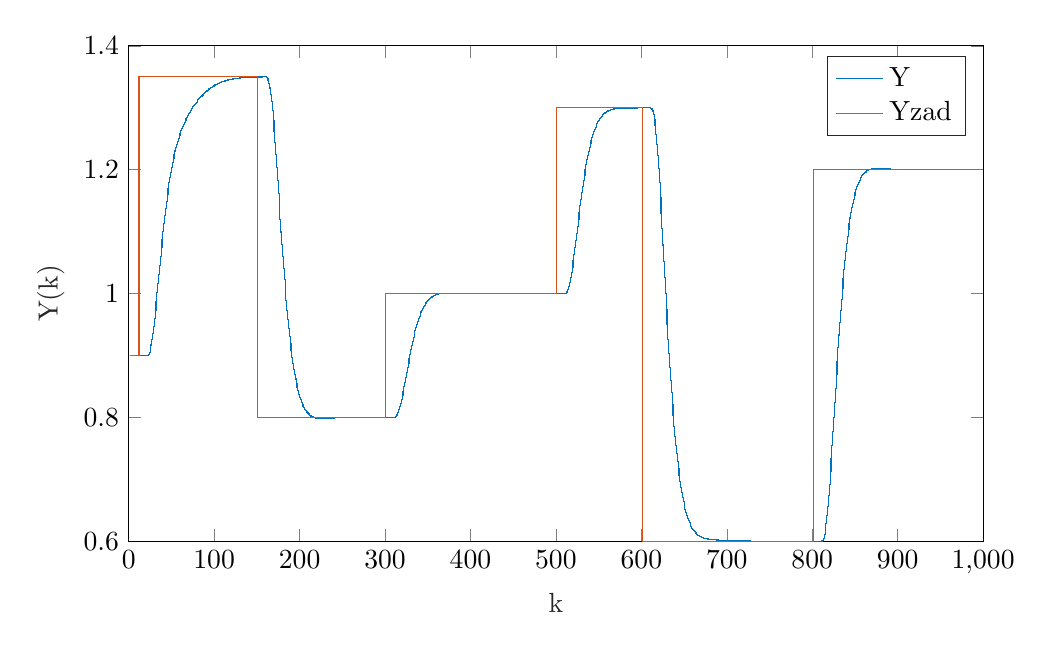
\begin{tikzpicture}

\begin{axis}[%
width=4.272in,
height=2.477in,
at={(0.717in,0.437in)},
scale only axis,
xmin=0,
xmax=1000,
xlabel style={font=\color{white!15!black}},
xlabel={k},
ymin=0.599989894805205,
ymax=1.4,
ylabel style={font=\color{white!15!black}},
ylabel={Y(k)},
axis background/.style={fill=white},
legend style={legend cell align=left, align=left, draw=white!15!black}
]
\addplot[const plot, color=mycolor1] table[row sep=crcr] {%
1	0.9\\
2	0.9\\
3	0.9\\
4	0.9\\
5	0.9\\
6	0.9\\
7	0.9\\
8	0.9\\
9	0.9\\
10	0.9\\
11	0.9\\
12	0.9\\
13	0.9\\
14	0.9\\
15	0.9\\
16	0.9\\
17	0.9\\
18	0.9\\
19	0.9\\
20	0.9\\
21	0.9\\
22	0.9003968325\\
23	0.901892448707372\\
24	0.904981890699363\\
25	0.90992361178901\\
26	0.916803293185557\\
27	0.925526543215358\\
28	0.935826971238976\\
29	0.947394980517016\\
30	0.95996069448629\\
31	0.973289547202598\\
32	0.987178329072141\\
33	1.00145164283678\\
34	1.01595508990297\\
35	1.03054682453519\\
36	1.04509559351457\\
37	1.05948292250313\\
38	1.07360450286326\\
39	1.08737103053098\\
40	1.100708523175\\
41	1.11355811620516\\
42	1.12587539856678\\
43	1.13762937907675\\
44	1.14880118771846\\
45	1.15938262174392\\
46	1.16937463682123\\
47	1.17878585930981\\
48	1.18763117117784\\
49	1.19593040051561\\
50	1.20370713674147\\
51	1.21098767940987\\
52	1.21780012218925\\
53	1.22417356842974\\
54	1.23013747127051\\
55	1.23572108903803\\
56	1.24095304543993\\
57	1.2458609835149\\
58	1.25047130226328\\
59	1.25480896520437\\
60	1.25889737067069\\
61	1.26275827436809\\
62	1.26641175553688\\
63	1.26987621889572\\
64	1.27316842539879\\
65	1.2763035456642\\
66	1.27929523071918\\
67	1.28215569544441\\
68	1.28489581077858\\
69	1.28752520136287\\
70	1.29005234586136\\
71	1.29248467768968\\
72	1.29482868432238\\
73	1.29709000373319\\
74	1.29927351685503\\
75	1.30138343523255\\
76	1.30342338328407\\
77	1.30539647479464\\
78	1.30730538343366\\
79	1.30915240723109\\
80	1.31093952706096\\
81	1.31266845927161\\
82	1.31434070267333\\
83	1.31595758014734\\
84	1.31752027517924\\
85	1.31902986364601\\
86	1.32048734120174\\
87	1.32189364661443\\
88	1.32324968140632\\
89	1.3245563261446\\
90	1.32581445371948\\
91	1.32702493993287\\
92	1.32818867170508\\
93	1.32930655318875\\
94	1.33037951006043\\
95	1.33140849224032\\
96	1.33239447527045\\
97	1.33333846056229\\
98	1.33424147470453\\
99	1.3351045680036\\
100	1.33592881241101\\
101	1.33671529897448\\
102	1.33746513493402\\
103	1.33817944056846\\
104	1.33885934588461\\
105	1.33950598722773\\
106	1.34012050388051\\
107	1.34070403470711\\
108	1.34125771488871\\
109	1.34178267278867\\
110	1.34228002697744\\
111	1.34275088344045\\
112	1.34319633298606\\
113	1.34361744886562\\
114	1.34401528461257\\
115	1.34439087210411\\
116	1.34474521984507\\
117	1.3450793114712\\
118	1.34539410446655\\
119	1.34569052908751\\
120	1.3459694874851\\
121	1.34623185301523\\
122	1.34647846972632\\
123	1.34671015201284\\
124	1.34692768442281\\
125	1.34713182160736\\
126	1.34732328840037\\
127	1.34750278001617\\
128	1.3476709623537\\
129	1.34782847239587\\
130	1.34797591869303\\
131	1.34811388192045\\
132	1.34824291549951\\
133	1.34836354627364\\
134	1.34847627522995\\
135	1.3485815782586\\
136	1.34867990694216\\
137	1.34877168936808\\
138	1.3488573309579\\
139	1.34893721530718\\
140	1.34901170503113\\
141	1.34908114261089\\
142	1.34914585123647\\
143	1.34920613564241\\
144	1.34926228293285\\
145	1.34931456339316\\
146	1.34936323128559\\
147	1.34940852562685\\
148	1.34945067094565\\
149	1.34948987801903\\
150	1.34952634458591\\
151	1.34956025603722\\
152	1.34959178608174\\
153	1.34962109738729\\
154	1.34964834219678\\
155	1.34967366291923\\
156	1.34969719269568\\
157	1.34971905594003\\
158	1.3497393688554\\
159	1.34975823992601\\
160	1.34977577038537\\
161	1.34939522235863\\
162	1.34790846197924\\
163	1.34472384182212\\
164	1.33942816473346\\
165	1.33183188534404\\
166	1.32191950451952\\
167	1.30979732275263\\
168	1.29565321805746\\
169	1.27972596970897\\
170	1.26228213643832\\
171	1.24359889081324\\
172	1.22395152863077\\
173	1.20360462786094\\
174	1.1828060378158\\
175	1.16178304531489\\
176	1.14074019837713\\
177	1.11985837560861\\
178	1.09929477599994\\
179	1.07918357335432\\
180	1.05963703531781\\
181	1.04074695162694\\
182	1.0225862518686\\
183	1.00521072149467\\
184	0.988660747450228\\
185	0.972963042691612\\
186	0.958132313004961\\
187	0.944172840628259\\
188	0.93107996782909\\
189	0.918841470280771\\
190	0.907438815202526\\
191	0.896848303101203\\
192	0.887042094828686\\
193	0.877989127757456\\
194	0.869655926343183\\
195	0.86200731332208\\
196	0.85500702838986\\
197	0.848618261515409\\
198	0.84280410794285\\
199	0.837527952127478\\
200	0.83275378781309\\
201	0.828446480866846\\
202	0.824571981093861\\
203	0.821097488882057\\
204	0.817991582128166\\
205	0.815224308483006\\
206	0.812767247539439\\
207	0.810593547178289\\
208	0.80867793789215\\
209	0.806996728528812\\
210	0.80552778653803\\
211	0.804250505469433\\
212	0.803145762156569\\
213	0.802195865732703\\
214	0.801384500357932\\
215	0.800696663293952\\
216	0.800118599741706\\
217	0.799637735657101\\
218	0.799242609579867\\
219	0.798922804349123\\
220	0.798668879435116\\
221	0.798472304488568\\
222	0.798325394595942\\
223	0.798221247629405\\
224	0.798153683993231\\
225	0.798117188992689\\
226	0.798106857986048\\
227	0.798118344424133\\
228	0.798147810834071\\
229	0.798191882763419\\
230	0.798247605667109\\
231	0.798312404691718\\
232	0.798384047288847\\
233	0.798460608571201\\
234	0.798540439310771\\
235	0.798622136467773\\
236	0.798704516131208\\
237	0.798786588746772\\
238	0.798867536504779\\
239	0.798946692759648\\
240	0.799023523352875\\
241	0.79909760971309\\
242	0.799168633609529\\
243	0.799236363438808\\
244	0.799300641929124\\
245	0.799361375150714\\
246	0.799418522726543\\
247	0.799472089142503\\
248	0.79952211606195\\
249	0.799568675554948\\
250	0.79961186415819\\
251	0.799651797687067\\
252	0.799688606726765\\
253	0.799722432734538\\
254	0.799753424690365\\
255	0.799781736238114\\
256	0.799807523263974\\
257	0.799830941863349\\
258	0.799852146651626\\
259	0.799871289378148\\
260	0.799888517806466\\
261	0.799903974827392\\
262	0.799917797774605\\
263	0.799930117915597\\
264	0.799941060093478\\
265	0.799950742497771\\
266	0.799959276544652\\
267	0.799966766849281\\
268	0.799973311274837\\
269	0.79997900104468\\
270	0.799983920905709\\
271	0.799988149332462\\
272	0.799991758762876\\
273	0.799994815857803\\
274	0.799997381777507\\
275	0.799999512469301\\
276	0.800001258961405\\
277	0.800002667658834\\
278	0.800003780637847\\
279	0.800004635936074\\
280	0.800005267835992\\
281	0.800005707139874\\
282	0.800005981434748\\
283	0.800006115346263\\
284	0.80000613078066\\
285	0.800006047154303\\
286	0.800005881610468\\
287	0.800005649223249\\
288	0.800005363188619\\
289	0.800005035002814\\
290	0.800004674628299\\
291	0.800004290647676\\
292	0.800003890405961\\
293	0.800003480141694\\
294	0.800003065107408\\
295	0.800002649679986\\
296	0.80000223746146\\
297	0.800001831370829\\
298	0.800001433727438\\
299	0.800001046326488\\
300	0.800000670507232\\
301	0.800000307214367\\
302	0.799999957053168\\
303	0.799999620338833\\
304	0.799999297140537\\
305	0.799998987320633\\
306	0.799998690569446\\
307	0.799998406436053\\
308	0.799998134355442\\
309	0.799997873672411\\
310	0.799997623662549\\
311	0.80020870466009\\
312	0.800963041331569\\
313	0.802458475066207\\
314	0.804793430253153\\
315	0.807994028131292\\
316	0.812035171382014\\
317	0.81685682539514\\
318	0.822376482267605\\
319	0.828498600034995\\
320	0.835121653464611\\
321	0.84214330675504\\
322	0.849464116879972\\
323	0.856990094392246\\
324	0.864634382481061\\
325	0.872318261892989\\
326	0.87997164651648\\
327	0.887533199995356\\
328	0.894950176068113\\
329	0.902178063124913\\
330	0.909180095681172\\
331	0.915926681234844\\
332	0.92239477961608\\
333	0.928567262896939\\
334	0.934432276755725\\
335	0.93998261852183\\
336	0.945215142668705\\
337	0.950130201219413\\
338	0.954731123550447\\
339	0.959023737864252\\
340	0.963015935250908\\
341	0.966717276085355\\
342	0.970138637681497\\
343	0.973291901494268\\
344	0.976189677722443\\
345	0.978845064884813\\
346	0.981271441784558\\
347	0.983482289212418\\
348	0.985491038745657\\
349	0.987310946058551\\
350	0.988954986256669\\
351	0.990435768870104\\
352	0.991765470281037\\
353	0.99295578151158\\
354	0.99401786945322\\
355	0.994962349775376\\
356	0.995799269904307\\
357	0.996538100612655\\
358	0.997187734902627\\
359	0.997756493001019\\
360	0.998252132411344\\
361	0.998681862086694\\
362	0.999052359896701\\
363	0.999369792662843\\
364	0.999639838128805\\
365	0.999867708316737\\
366	1.00005817379653\\
367	1.00021558846401\\
368	1.00034391448574\\
369	1.00044674712328\\
370	1.00052733919891\\
371	1.00058862500816\\
372	1.00063324352302\\
373	1.00066356076301\\
374	1.00068169124069\\
375	1.00068951841364\\
376	1.00068871409642\\
377	1.00068075680521\\
378	1.00066694902304\\
379	1.00064843338739\\
380	1.00062620781249\\
381	1.00060113956812\\
382	1.00057397834356\\
383	1.00054536833163\\
384	1.00051585937164\\
385	1.00048591719381\\
386	1.00045593280966\\
387	1.00042623109455\\
388	1.00039707860896\\
389	1.00036869070546\\
390	1.00034123796777\\
391	1.00031485202741\\
392	1.00028963080241\\
393	1.00026564320104\\
394	1.00024293333172\\
395	1.00022152425882\\
396	1.00020142134176\\
397	1.00018261519303\\
398	1.00016508428876\\
399	1.00014879726327\\
400	1.00013371491716\\
401	1.00011979196649\\
402	1.00010697855848\\
403	1.0000952215776\\
404	1.00008446576377\\
405	1.00007465466292\\
406	1.00006573142832\\
407	1.00005763948965\\
408	1.00005032310517\\
409	1.00004372781118\\
410	1.00003780078135\\
411	1.0000324911076\\
412	1.00002775001275\\
413	1.00002353100448\\
414	1.00001978997884\\
415	1.00001648528089\\
416	1.00001357772901\\
417	1.00001103060895\\
418	1.00000880964275\\
419	1.00000688293714\\
420	1.00000522091551\\
421	1.00000379623691\\
422	1.00000258370517\\
423	1.00000156017082\\
424	1.00000070442803\\
425	0.999999997108525\\
426	0.999999420574089\\
427	0.999998958809118\\
428	0.999998597314252\\
429	0.999998323002089\\
430	0.999998124095723\\
431	0.999997990030684\\
432	0.999997911360763\\
433	0.99999787966804\\
434	0.999997887477355\\
435	0.999997928175388\\
436	0.9999979959344\\
437	0.999998085640662\\
438	0.999998192827527\\
439	0.99999831361307\\
440	0.999998444642168\\
441	0.999998583032888\\
442	0.99999872632701\\
443	0.999998872444509\\
444	0.999999019641801\\
445	0.999999166473553\\
446	0.999999311757858\\
447	0.999999454544557\\
448	0.999999594086526\\
449	0.999999729813703\\
450	0.999999861309676\\
451	0.999999988290633\\
452	1.00000011058649\\
453	1.00000022812403\\
454	1.00000034091187\\
455	1.00000044902708\\
456	1.00000055260339\\
457	1.00000065182071\\
458	1.00000074689591\\
459	1.00000083807474\\
460	1.00000092562472\\
461	1.00000100982892\\
462	1.00000109098055\\
463	1.0000011693782\\
464	1.00000124532167\\
465	1.00000131910834\\
466	1.00000139102993\\
467	1.00000146136968\\
468	1.00000153039967\\
469	1.00000159837853\\
470	1.00000166554919\\
471	1.00000173213674\\
472	1.00000179834631\\
473	1.00000186436097\\
474	1.00000193033953\\
475	1.00000199641415\\
476	1.00000206268802\\
477	1.00000212923308\\
478	1.00000219608829\\
479	1.00000226325885\\
480	1.00000233071653\\
481	1.00000239840122\\
482	1.00000246622348\\
483	1.0000025340679\\
484	1.00000260179711\\
485	1.00000266925613\\
486	1.00000273627686\\
487	1.00000280258547\\
488	1.00000286768184\\
489	1.00000293081791\\
490	1.00000299103316\\
491	1.00000304721891\\
492	1.00000309819273\\
493	1.00000314277134\\
494	1.00000317983506\\
495	1.00000320838049\\
496	1.00000322755999\\
497	1.00000323670833\\
498	1.00000323535755\\
499	1.00000322324153\\
500	1.0000032002921\\
501	1.00000316662844\\
502	1.00000312254151\\
503	1.00000306847489\\
504	1.00000300500355\\
505	1.00000293281151\\
506	1.00000285266939\\
507	1.00000276541257\\
508	1.00000267192046\\
509	1.00000257309733\\
510	1.00000246985501\\
511	1.00031934476166\\
512	1.00145108691488\\
513	1.00369446049492\\
514	1.00719710415283\\
515	1.01199820176163\\
516	1.01806010928566\\
517	1.02529277666284\\
518	1.03357244378886\\
519	1.04275579935305\\
520	1.05268403553515\\
521	1.06318947139969\\
522	1.0741156948062\\
523	1.08532445260438\\
524	1.0966898713515\\
525	1.10809773548214\\
526	1.11944629067114\\
527	1.13064647259698\\
528	1.14162171575628\\
529	1.15230746361552\\
530	1.16265048153401\\
531	1.17260805762892\\
532	1.18214714057193\\
533	1.19124343368522\\
534	1.19988046769547\\
535	1.20804868054314\\
536	1.21574452700461\\
537	1.22296963382499\\
538	1.22973001060312\\
539	1.23603532249151\\
540	1.24189822760965\\
541	1.24733377970762\\
542	1.25235889488908\\
543	1.25699187997175\\
544	1.26125201922014\\
545	1.26515921564303\\
546	1.26873368273632\\
547	1.2719956824154\\
548	1.274965304876\\
549	1.27766228621351\\
550	1.28010585979054\\
551	1.28231463754991\\
552	1.28430651770762\\
553	1.28609861551602\\
554	1.28770721405004\\
555	1.28914773223293\\
556	1.29043470757595\\
557	1.29158179135508\\
558	1.29260175418487\\
559	1.29350650017264\\
560	1.29430708804406\\
561	1.29501375782416\\
562	1.29563596183483\\
563	1.29618239893177\\
564	1.29666105105101\\
565	1.29707922126773\\
566	1.29744357268995\\
567	1.29776016761593\\
568	1.29803450647967\\
569	1.29827156619268\\
570	1.29847583756445\\
571	1.2986513615491\\
572	1.29880176412204\\
573	1.29893028963996\\
574	1.29903983257914\\
575	1.29913296758372\\
576	1.29921197778575\\
577	1.29927888138493\\
578	1.29933545649701\\
579	1.29938326429789\\
580	1.29942367050409\\
581	1.29945786524228\\
582	1.29948688136862\\
583	1.29951161130589\\
584	1.29953282247043\\
585	1.29955117136448\\
586	1.29956721641095\\
587	1.29958142960804\\
588	1.29959420708113\\
589	1.2996058786077\\
590	1.29961671618948\\
591	1.29962694174356\\
592	1.2996367339816\\
593	1.29964623454293\\
594	1.29965555344462\\
595	1.29966477390764\\
596	1.29967395661527\\
597	1.29968314345619\\
598	1.29969236080134\\
599	1.29970162236022\\
600	1.29971093165898\\
601	1.29972028417946\\
602	1.29972966919541\\
603	1.29973907133879\\
604	1.29974847192674\\
605	1.29975785007679\\
606	1.29976718363552\\
607	1.29977644994369\\
608	1.29978562645825\\
609	1.29979469125016\\
610	1.29980362339462\\
611	1.29941556266315\\
612	1.29792225554377\\
613	1.29473194726897\\
614	1.28935516999022\\
615	1.28140033685273\\
616	1.27065127523557\\
617	1.25710168068112\\
618	1.24089161809186\\
619	1.22225868384317\\
620	1.20150080223205\\
621	1.17896567493168\\
622	1.15503855447965\\
623	1.1300876373888\\
624	1.10443308152663\\
625	1.07836282908965\\
626	1.05214085632974\\
627	1.02600443649406\\
628	1.00016293046436\\
629	0.974797706997828\\
630	0.950062879505682\\
631	0.926086596074946\\
632	0.90297265453412\\
633	0.880802306365286\\
634	0.859636207822698\\
635	0.839516476292898\\
636	0.820468778708976\\
637	0.802504384867145\\
638	0.785622138357718\\
639	0.769810313202906\\
640	0.755048336105972\\
641	0.741308363195623\\
642	0.728556706887341\\
643	0.716755113453629\\
644	0.705861895478301\\
645	0.69583292587002\\
646	0.686622501770582\\
647	0.678184087707871\\
648	0.670470947866071\\
649	0.663436677499216\\
650	0.657035643395001\\
651	0.651223342980189\\
652	0.645956691206522\\
653	0.641194243813139\\
654	0.636896364963845\\
655	0.633025346632661\\
656	0.629545486479357\\
657	0.626423130333534\\
658	0.623626684802405\\
659	0.621126604941351\\
660	0.618895361382973\\
661	0.616907390812767\\
662	0.615139033209436\\
663	0.613568458835633\\
664	0.612175587570259\\
665	0.61094200281516\\
666	0.609850861885771\\
667	0.608886804505065\\
668	0.608035860761004\\
669	0.607285359657557\\
670	0.606623839185912\\
671	0.606040958663736\\
672	0.605527413933979\\
673	0.605074855878856\\
674	0.604675812587223\\
675	0.604323615412832\\
676	0.604012329075237\\
677	0.603736685882769\\
678	0.603492024096568\\
679	0.603274230404386\\
680	0.603079686431571\\
681	0.602905219183239\\
682	0.602748055285422\\
683	0.602605778872964\\
684	0.602476292957208\\
685	0.602357784096303\\
686	0.602248690184616\\
687	0.602147671028894\\
688	0.602053581628177\\
689	0.601965448162518\\
690	0.60188244644627\\
691	0.601803882626775\\
692	0.601729175929975\\
693	0.601657843271854\\
694	0.601589485569518\\
695	0.601523775598809\\
696	0.601460447257033\\
697	0.601399286099969\\
698	0.601340121032097\\
699	0.601282817038029\\
700	0.601227268851615\\
701	0.601173395467191\\
702	0.601121135404924\\
703	0.601070442649352\\
704	0.601021283186879\\
705	0.600973632074359\\
706	0.600927470976788\\
707	0.600882786117759\\
708	0.600839566591537\\
709	0.600797802990508\\
710	0.600757486306342\\
711	0.600718607067418\\
712	0.600681154678985\\
713	0.600645116936147\\
714	0.60061047968305\\
715	0.600577226594724\\
716	0.60054533906077\\
717	0.600514796152644\\
718	0.600485574658561\\
719	0.600457649172125\\
720	0.600430992222664\\
721	0.60040557443694\\
722	0.600381364723376\\
723	0.60035833047133\\
724	0.600336437759108\\
725	0.600315651565467\\
726	0.600295935980306\\
727	0.60027725441104\\
728	0.600259569781875\\
729	0.600242844723815\\
730	0.600227041753772\\
731	0.600212123441604\\
732	0.600198052564295\\
733	0.600184792246817\\
734	0.600172306089508\\
735	0.600160558281998\\
736	0.600149513703935\\
737	0.600139138012875\\
738	0.600129397719866\\
739	0.600120260253289\\
740	0.600111694011635\\
741	0.600103668405917\\
742	0.600096153892446\\
743	0.600089121996725\\
744	0.6000825453292\\
745	0.600076397593617\\
746	0.600070653588705\\
747	0.600065289203889\\
748	0.600060281409697\\
749	0.600055608243509\\
750	0.600051248791261\\
751	0.600047183165661\\
752	0.600043392481456\\
753	0.600039858828253\\
754	0.600036565241342\\
755	0.600033495670951\\
756	0.600030634950315\\
757	0.600027968762917\\
758	0.600025483609215\\
759	0.600023166773153\\
760	0.600021006288709\\
761	0.60001899090672\\
762	0.600017110062196\\
763	0.600015353842302\\
764	0.600013712955184\\
765	0.600012178699787\\
766	0.600010742936797\\
767	0.600009398060826\\
768	0.600008136973957\\
769	0.60000695306073\\
770	0.600005840164682\\
771	0.600004792566513\\
772	0.600003804963966\\
773	0.600002872453497\\
774	0.600001990513822\\
775	0.600001154991378\\
776	0.600000362087562\\
777	0.599999608347308\\
778	0.599998890648128\\
779	0.59999820618852\\
780	0.599997552474765\\
781	0.599996927305558\\
782	0.599996328754206\\
783	0.599995755148503\\
784	0.599995205048689\\
785	0.599994677224091\\
786	0.599994170629091\\
787	0.599993684561473\\
788	0.599993218912445\\
789	0.599992774282481\\
790	0.599992352002902\\
791	0.599991954089892\\
792	0.599991583114246\\
793	0.599991241996072\\
794	0.599990933777785\\
795	0.599990661408311\\
796	0.599990427557169\\
797	0.599990234467356\\
798	0.599990083849533\\
799	0.599989976815885\\
800	0.599989913849673\\
801	0.599989894805205\\
802	0.599989918932542\\
803	0.5999899849213\\
804	0.599990090958292\\
805	0.59999023479434\\
806	0.599990413816225\\
807	0.599990625120433\\
808	0.599990865586019\\
809	0.59999113194453\\
810	0.599991420845449\\
811	0.60038856050463\\
812	0.601890768286105\\
813	0.605089769535175\\
814	0.610451665335784\\
815	0.618249051814754\\
816	0.628546953001725\\
817	0.641263734412769\\
818	0.656218103987006\\
819	0.673165059829866\\
820	0.6918230826383\\
821	0.711894417596871\\
822	0.733079925045017\\
823	0.755089684461548\\
824	0.777650298680413\\
825	0.800509653752882\\
826	0.823439735631908\\
827	0.84623798070894\\
828	0.868727537393502\\
829	0.890756735715544\\
830	0.912197997571691\\
831	0.932946368675555\\
832	0.952917812041367\\
833	0.972047369934068\\
834	0.990287275044553\\
835	1.00760507089159\\
836	1.02398178505713\\
837	1.03941018597612\\
838	1.05389314393602\\
839	1.06744210913612\\
840	1.08007571366287\\
841	1.09181849968884\\
842	1.10269977280559\\
843	1.11275257691699\\
844	1.12201278535716\\
845	1.13051830170134\\
846	1.13830836298441\\
847	1.14542293763014\\
848	1.15190221024431\\
849	1.15778614547194\\
850	1.16311412331249\\
851	1.16792463858526\\
852	1.17225505760901\\
853	1.17614142557899\\
854	1.17961831857158\\
855	1.18271873456643\\
856	1.18547401833628\\
857	1.18791381550689\\
858	1.19006605152745\\
859	1.19195693171049\\
860	1.19361095889648\\
861	1.19505096567063\\
862	1.19629815840567\\
863	1.19737217072564\\
864	1.19829112428034\\
865	1.19907169499079\\
866	1.19972918317133\\
867	1.20027758615712\\
868	1.2007296722665\\
869	1.20109705510773\\
870	1.20139026740082\\
871	1.20161883362818\\
872	1.20179134095448\\
873	1.20191550796763\\
874	1.20199825089055\\
875	1.20204574699841\\
876	1.20206349504968\\
877	1.20205637260287\\
878	1.20202869014477\\
879	1.20198424200189\\
880	1.20192635404529\\
881	1.20185792823087\\
882	1.2017814840431\\
883	1.20169919693132\\
884	1.20161293384427\\
885	1.20152428598088\\
886	1.20143459888484\\
887	1.20134500001682\\
888	1.20125642394175\\
889	1.20116963527084\\
890	1.20108524949757\\
891	1.20100375186567\\
892	1.20092551440436\\
893	1.20085081126255\\
894	1.20077983246911\\
895	1.20071269624151\\
896	1.20064945995963\\
897	1.20059012991575\\
898	1.20053466994576\\
899	1.20048300904074\\
900	1.20043504803176\\
901	1.20039066543497\\
902	1.20034972253797\\
903	1.20031206780277\\
904	1.20027754065501\\
905	1.2002459747239\\
906	1.20021720059189\\
907	1.20019104810861\\
908	1.20016734831854\\
909	1.20014593504795\\
910	1.2001266461922\\
911	1.20010932474072\\
912	1.20009381957365\\
913	1.20007998606038\\
914	1.20006768648749\\
915	1.20005679034062\\
916	1.20004717446201\\
917	1.20003872310341\\
918	1.20003132789142\\
919	1.2000248877207\\
920	1.20001930858833\\
921	1.20001450338122\\
922	1.20001039162665\\
923	1.20000689921507\\
924	1.20000395810264\\
925	1.20000150600025\\
926	1.19999948605447\\
927	1.19999784652536\\
928	1.1999965404649\\
929	1.19999552539959\\
930	1.19999476301956\\
931	1.19999421887665\\
932	1.19999386209304\\
933	1.19999366508162\\
934	1.19999360327925\\
935	1.19999365489343\\
936	1.19999380066273\\
937	1.19999402363139\\
938	1.19999430893778\\
939	1.19999464361684\\
940	1.19999501641613\\
941	1.19999541762502\\
942	1.19999583891682\\
943	1.19999627320308\\
944	1.19999671449968\\
945	1.19999715780409\\
946	1.19999759898313\\
947	1.19999803467075\\
948	1.19999846217507\\
949	1.19999887939416\\
950	1.19999928473996\\
951	1.19999967706971\\
952	1.20000005562432\\
953	1.20000041997322\\
954	1.20000076996508\\
955	1.20000110568385\\
956	1.20000142740984\\
957	1.20000173558517\\
958	1.20000203078329\\
959	1.20000231368217\\
960	1.20000258504072\\
961	1.20000284567809\\
962	1.20000309645566\\
963	1.20000333826118\\
964	1.20000357199497\\
965	1.20000379855781\\
966	1.20000401884029\\
967	1.20000423371338\\
968	1.20000444402004\\
969	1.20000465056756\\
970	1.20000485412052\\
971	1.20000505539419\\
972	1.20000525504808\\
973	1.2000054536796\\
974	1.20000565181756\\
975	1.20000584991537\\
976	1.20000604834419\\
977	1.20000624738603\\
978	1.20000644722804\\
979	1.2000066479586\\
980	1.20000684956633\\
981	1.20000705194224\\
982	1.20000725488508\\
983	1.20000745810948\\
984	1.20000766125631\\
985	1.20000786390465\\
986	1.20000806558475\\
987	1.20000826560888\\
988	1.20000846281098\\
989	1.20000865542088\\
990	1.20000884104408\\
991	1.20000901675049\\
992	1.200009179248\\
993	1.20000932508655\\
994	1.20000945085906\\
995	1.20000955337912\\
996	1.20000962982542\\
997	1.20000967784925\\
998	1.20000969564556\\
999	1.20000968199077\\
1000	1.20000963625161\\
};
\addlegendentry{Y}

\addplot[const plot, color=mycolor2] table[row sep=crcr] {%
1	0.9\\
2	0.9\\
3	0.9\\
4	0.9\\
5	0.9\\
6	0.9\\
7	0.9\\
8	0.9\\
9	0.9\\
10	0.9\\
11	0.9\\
12	1.35\\
13	1.35\\
14	1.35\\
15	1.35\\
16	1.35\\
17	1.35\\
18	1.35\\
19	1.35\\
20	1.35\\
21	1.35\\
22	1.35\\
23	1.35\\
24	1.35\\
25	1.35\\
26	1.35\\
27	1.35\\
28	1.35\\
29	1.35\\
30	1.35\\
31	1.35\\
32	1.35\\
33	1.35\\
34	1.35\\
35	1.35\\
36	1.35\\
37	1.35\\
38	1.35\\
39	1.35\\
40	1.35\\
41	1.35\\
42	1.35\\
43	1.35\\
44	1.35\\
45	1.35\\
46	1.35\\
47	1.35\\
48	1.35\\
49	1.35\\
50	1.35\\
51	1.35\\
52	1.35\\
53	1.35\\
54	1.35\\
55	1.35\\
56	1.35\\
57	1.35\\
58	1.35\\
59	1.35\\
60	1.35\\
61	1.35\\
62	1.35\\
63	1.35\\
64	1.35\\
65	1.35\\
66	1.35\\
67	1.35\\
68	1.35\\
69	1.35\\
70	1.35\\
71	1.35\\
72	1.35\\
73	1.35\\
74	1.35\\
75	1.35\\
76	1.35\\
77	1.35\\
78	1.35\\
79	1.35\\
80	1.35\\
81	1.35\\
82	1.35\\
83	1.35\\
84	1.35\\
85	1.35\\
86	1.35\\
87	1.35\\
88	1.35\\
89	1.35\\
90	1.35\\
91	1.35\\
92	1.35\\
93	1.35\\
94	1.35\\
95	1.35\\
96	1.35\\
97	1.35\\
98	1.35\\
99	1.35\\
100	1.35\\
101	1.35\\
102	1.35\\
103	1.35\\
104	1.35\\
105	1.35\\
106	1.35\\
107	1.35\\
108	1.35\\
109	1.35\\
110	1.35\\
111	1.35\\
112	1.35\\
113	1.35\\
114	1.35\\
115	1.35\\
116	1.35\\
117	1.35\\
118	1.35\\
119	1.35\\
120	1.35\\
121	1.35\\
122	1.35\\
123	1.35\\
124	1.35\\
125	1.35\\
126	1.35\\
127	1.35\\
128	1.35\\
129	1.35\\
130	1.35\\
131	1.35\\
132	1.35\\
133	1.35\\
134	1.35\\
135	1.35\\
136	1.35\\
137	1.35\\
138	1.35\\
139	1.35\\
140	1.35\\
141	1.35\\
142	1.35\\
143	1.35\\
144	1.35\\
145	1.35\\
146	1.35\\
147	1.35\\
148	1.35\\
149	1.35\\
150	1.35\\
151	0.8\\
152	0.8\\
153	0.8\\
154	0.8\\
155	0.8\\
156	0.8\\
157	0.8\\
158	0.8\\
159	0.8\\
160	0.8\\
161	0.8\\
162	0.8\\
163	0.8\\
164	0.8\\
165	0.8\\
166	0.8\\
167	0.8\\
168	0.8\\
169	0.8\\
170	0.8\\
171	0.8\\
172	0.8\\
173	0.8\\
174	0.8\\
175	0.8\\
176	0.8\\
177	0.8\\
178	0.8\\
179	0.8\\
180	0.8\\
181	0.8\\
182	0.8\\
183	0.8\\
184	0.8\\
185	0.8\\
186	0.8\\
187	0.8\\
188	0.8\\
189	0.8\\
190	0.8\\
191	0.8\\
192	0.8\\
193	0.8\\
194	0.8\\
195	0.8\\
196	0.8\\
197	0.8\\
198	0.8\\
199	0.8\\
200	0.8\\
201	0.8\\
202	0.8\\
203	0.8\\
204	0.8\\
205	0.8\\
206	0.8\\
207	0.8\\
208	0.8\\
209	0.8\\
210	0.8\\
211	0.8\\
212	0.8\\
213	0.8\\
214	0.8\\
215	0.8\\
216	0.8\\
217	0.8\\
218	0.8\\
219	0.8\\
220	0.8\\
221	0.8\\
222	0.8\\
223	0.8\\
224	0.8\\
225	0.8\\
226	0.8\\
227	0.8\\
228	0.8\\
229	0.8\\
230	0.8\\
231	0.8\\
232	0.8\\
233	0.8\\
234	0.8\\
235	0.8\\
236	0.8\\
237	0.8\\
238	0.8\\
239	0.8\\
240	0.8\\
241	0.8\\
242	0.8\\
243	0.8\\
244	0.8\\
245	0.8\\
246	0.8\\
247	0.8\\
248	0.8\\
249	0.8\\
250	0.8\\
251	0.8\\
252	0.8\\
253	0.8\\
254	0.8\\
255	0.8\\
256	0.8\\
257	0.8\\
258	0.8\\
259	0.8\\
260	0.8\\
261	0.8\\
262	0.8\\
263	0.8\\
264	0.8\\
265	0.8\\
266	0.8\\
267	0.8\\
268	0.8\\
269	0.8\\
270	0.8\\
271	0.8\\
272	0.8\\
273	0.8\\
274	0.8\\
275	0.8\\
276	0.8\\
277	0.8\\
278	0.8\\
279	0.8\\
280	0.8\\
281	0.8\\
282	0.8\\
283	0.8\\
284	0.8\\
285	0.8\\
286	0.8\\
287	0.8\\
288	0.8\\
289	0.8\\
290	0.8\\
291	0.8\\
292	0.8\\
293	0.8\\
294	0.8\\
295	0.8\\
296	0.8\\
297	0.8\\
298	0.8\\
299	0.8\\
300	0.8\\
301	1\\
302	1\\
303	1\\
304	1\\
305	1\\
306	1\\
307	1\\
308	1\\
309	1\\
310	1\\
311	1\\
312	1\\
313	1\\
314	1\\
315	1\\
316	1\\
317	1\\
318	1\\
319	1\\
320	1\\
321	1\\
322	1\\
323	1\\
324	1\\
325	1\\
326	1\\
327	1\\
328	1\\
329	1\\
330	1\\
331	1\\
332	1\\
333	1\\
334	1\\
335	1\\
336	1\\
337	1\\
338	1\\
339	1\\
340	1\\
341	1\\
342	1\\
343	1\\
344	1\\
345	1\\
346	1\\
347	1\\
348	1\\
349	1\\
350	1\\
351	1\\
352	1\\
353	1\\
354	1\\
355	1\\
356	1\\
357	1\\
358	1\\
359	1\\
360	1\\
361	1\\
362	1\\
363	1\\
364	1\\
365	1\\
366	1\\
367	1\\
368	1\\
369	1\\
370	1\\
371	1\\
372	1\\
373	1\\
374	1\\
375	1\\
376	1\\
377	1\\
378	1\\
379	1\\
380	1\\
381	1\\
382	1\\
383	1\\
384	1\\
385	1\\
386	1\\
387	1\\
388	1\\
389	1\\
390	1\\
391	1\\
392	1\\
393	1\\
394	1\\
395	1\\
396	1\\
397	1\\
398	1\\
399	1\\
400	1\\
401	1\\
402	1\\
403	1\\
404	1\\
405	1\\
406	1\\
407	1\\
408	1\\
409	1\\
410	1\\
411	1\\
412	1\\
413	1\\
414	1\\
415	1\\
416	1\\
417	1\\
418	1\\
419	1\\
420	1\\
421	1\\
422	1\\
423	1\\
424	1\\
425	1\\
426	1\\
427	1\\
428	1\\
429	1\\
430	1\\
431	1\\
432	1\\
433	1\\
434	1\\
435	1\\
436	1\\
437	1\\
438	1\\
439	1\\
440	1\\
441	1\\
442	1\\
443	1\\
444	1\\
445	1\\
446	1\\
447	1\\
448	1\\
449	1\\
450	1\\
451	1\\
452	1\\
453	1\\
454	1\\
455	1\\
456	1\\
457	1\\
458	1\\
459	1\\
460	1\\
461	1\\
462	1\\
463	1\\
464	1\\
465	1\\
466	1\\
467	1\\
468	1\\
469	1\\
470	1\\
471	1\\
472	1\\
473	1\\
474	1\\
475	1\\
476	1\\
477	1\\
478	1\\
479	1\\
480	1\\
481	1\\
482	1\\
483	1\\
484	1\\
485	1\\
486	1\\
487	1\\
488	1\\
489	1\\
490	1\\
491	1\\
492	1\\
493	1\\
494	1\\
495	1\\
496	1\\
497	1\\
498	1\\
499	1\\
500	1\\
501	1.3\\
502	1.3\\
503	1.3\\
504	1.3\\
505	1.3\\
506	1.3\\
507	1.3\\
508	1.3\\
509	1.3\\
510	1.3\\
511	1.3\\
512	1.3\\
513	1.3\\
514	1.3\\
515	1.3\\
516	1.3\\
517	1.3\\
518	1.3\\
519	1.3\\
520	1.3\\
521	1.3\\
522	1.3\\
523	1.3\\
524	1.3\\
525	1.3\\
526	1.3\\
527	1.3\\
528	1.3\\
529	1.3\\
530	1.3\\
531	1.3\\
532	1.3\\
533	1.3\\
534	1.3\\
535	1.3\\
536	1.3\\
537	1.3\\
538	1.3\\
539	1.3\\
540	1.3\\
541	1.3\\
542	1.3\\
543	1.3\\
544	1.3\\
545	1.3\\
546	1.3\\
547	1.3\\
548	1.3\\
549	1.3\\
550	1.3\\
551	1.3\\
552	1.3\\
553	1.3\\
554	1.3\\
555	1.3\\
556	1.3\\
557	1.3\\
558	1.3\\
559	1.3\\
560	1.3\\
561	1.3\\
562	1.3\\
563	1.3\\
564	1.3\\
565	1.3\\
566	1.3\\
567	1.3\\
568	1.3\\
569	1.3\\
570	1.3\\
571	1.3\\
572	1.3\\
573	1.3\\
574	1.3\\
575	1.3\\
576	1.3\\
577	1.3\\
578	1.3\\
579	1.3\\
580	1.3\\
581	1.3\\
582	1.3\\
583	1.3\\
584	1.3\\
585	1.3\\
586	1.3\\
587	1.3\\
588	1.3\\
589	1.3\\
590	1.3\\
591	1.3\\
592	1.3\\
593	1.3\\
594	1.3\\
595	1.3\\
596	1.3\\
597	1.3\\
598	1.3\\
599	1.3\\
600	1.3\\
601	0.6\\
602	0.6\\
603	0.6\\
604	0.6\\
605	0.6\\
606	0.6\\
607	0.6\\
608	0.6\\
609	0.6\\
610	0.6\\
611	0.6\\
612	0.6\\
613	0.6\\
614	0.6\\
615	0.6\\
616	0.6\\
617	0.6\\
618	0.6\\
619	0.6\\
620	0.6\\
621	0.6\\
622	0.6\\
623	0.6\\
624	0.6\\
625	0.6\\
626	0.6\\
627	0.6\\
628	0.6\\
629	0.6\\
630	0.6\\
631	0.6\\
632	0.6\\
633	0.6\\
634	0.6\\
635	0.6\\
636	0.6\\
637	0.6\\
638	0.6\\
639	0.6\\
640	0.6\\
641	0.6\\
642	0.6\\
643	0.6\\
644	0.6\\
645	0.6\\
646	0.6\\
647	0.6\\
648	0.6\\
649	0.6\\
650	0.6\\
651	0.6\\
652	0.6\\
653	0.6\\
654	0.6\\
655	0.6\\
656	0.6\\
657	0.6\\
658	0.6\\
659	0.6\\
660	0.6\\
661	0.6\\
662	0.6\\
663	0.6\\
664	0.6\\
665	0.6\\
666	0.6\\
667	0.6\\
668	0.6\\
669	0.6\\
670	0.6\\
671	0.6\\
672	0.6\\
673	0.6\\
674	0.6\\
675	0.6\\
676	0.6\\
677	0.6\\
678	0.6\\
679	0.6\\
680	0.6\\
681	0.6\\
682	0.6\\
683	0.6\\
684	0.6\\
685	0.6\\
686	0.6\\
687	0.6\\
688	0.6\\
689	0.6\\
690	0.6\\
691	0.6\\
692	0.6\\
693	0.6\\
694	0.6\\
695	0.6\\
696	0.6\\
697	0.6\\
698	0.6\\
699	0.6\\
700	0.6\\
701	0.6\\
702	0.6\\
703	0.6\\
704	0.6\\
705	0.6\\
706	0.6\\
707	0.6\\
708	0.6\\
709	0.6\\
710	0.6\\
711	0.6\\
712	0.6\\
713	0.6\\
714	0.6\\
715	0.6\\
716	0.6\\
717	0.6\\
718	0.6\\
719	0.6\\
720	0.6\\
721	0.6\\
722	0.6\\
723	0.6\\
724	0.6\\
725	0.6\\
726	0.6\\
727	0.6\\
728	0.6\\
729	0.6\\
730	0.6\\
731	0.6\\
732	0.6\\
733	0.6\\
734	0.6\\
735	0.6\\
736	0.6\\
737	0.6\\
738	0.6\\
739	0.6\\
740	0.6\\
741	0.6\\
742	0.6\\
743	0.6\\
744	0.6\\
745	0.6\\
746	0.6\\
747	0.6\\
748	0.6\\
749	0.6\\
750	0.6\\
751	0.6\\
752	0.6\\
753	0.6\\
754	0.6\\
755	0.6\\
756	0.6\\
757	0.6\\
758	0.6\\
759	0.6\\
760	0.6\\
761	0.6\\
762	0.6\\
763	0.6\\
764	0.6\\
765	0.6\\
766	0.6\\
767	0.6\\
768	0.6\\
769	0.6\\
770	0.6\\
771	0.6\\
772	0.6\\
773	0.6\\
774	0.6\\
775	0.6\\
776	0.6\\
777	0.6\\
778	0.6\\
779	0.6\\
780	0.6\\
781	0.6\\
782	0.6\\
783	0.6\\
784	0.6\\
785	0.6\\
786	0.6\\
787	0.6\\
788	0.6\\
789	0.6\\
790	0.6\\
791	0.6\\
792	0.6\\
793	0.6\\
794	0.6\\
795	0.6\\
796	0.6\\
797	0.6\\
798	0.6\\
799	0.6\\
800	0.6\\
801	1.2\\
802	1.2\\
803	1.2\\
804	1.2\\
805	1.2\\
806	1.2\\
807	1.2\\
808	1.2\\
809	1.2\\
810	1.2\\
811	1.2\\
812	1.2\\
813	1.2\\
814	1.2\\
815	1.2\\
816	1.2\\
817	1.2\\
818	1.2\\
819	1.2\\
820	1.2\\
821	1.2\\
822	1.2\\
823	1.2\\
824	1.2\\
825	1.2\\
826	1.2\\
827	1.2\\
828	1.2\\
829	1.2\\
830	1.2\\
831	1.2\\
832	1.2\\
833	1.2\\
834	1.2\\
835	1.2\\
836	1.2\\
837	1.2\\
838	1.2\\
839	1.2\\
840	1.2\\
841	1.2\\
842	1.2\\
843	1.2\\
844	1.2\\
845	1.2\\
846	1.2\\
847	1.2\\
848	1.2\\
849	1.2\\
850	1.2\\
851	1.2\\
852	1.2\\
853	1.2\\
854	1.2\\
855	1.2\\
856	1.2\\
857	1.2\\
858	1.2\\
859	1.2\\
860	1.2\\
861	1.2\\
862	1.2\\
863	1.2\\
864	1.2\\
865	1.2\\
866	1.2\\
867	1.2\\
868	1.2\\
869	1.2\\
870	1.2\\
871	1.2\\
872	1.2\\
873	1.2\\
874	1.2\\
875	1.2\\
876	1.2\\
877	1.2\\
878	1.2\\
879	1.2\\
880	1.2\\
881	1.2\\
882	1.2\\
883	1.2\\
884	1.2\\
885	1.2\\
886	1.2\\
887	1.2\\
888	1.2\\
889	1.2\\
890	1.2\\
891	1.2\\
892	1.2\\
893	1.2\\
894	1.2\\
895	1.2\\
896	1.2\\
897	1.2\\
898	1.2\\
899	1.2\\
900	1.2\\
901	1.2\\
902	1.2\\
903	1.2\\
904	1.2\\
905	1.2\\
906	1.2\\
907	1.2\\
908	1.2\\
909	1.2\\
910	1.2\\
911	1.2\\
912	1.2\\
913	1.2\\
914	1.2\\
915	1.2\\
916	1.2\\
917	1.2\\
918	1.2\\
919	1.2\\
920	1.2\\
921	1.2\\
922	1.2\\
923	1.2\\
924	1.2\\
925	1.2\\
926	1.2\\
927	1.2\\
928	1.2\\
929	1.2\\
930	1.2\\
931	1.2\\
932	1.2\\
933	1.2\\
934	1.2\\
935	1.2\\
936	1.2\\
937	1.2\\
938	1.2\\
939	1.2\\
940	1.2\\
941	1.2\\
942	1.2\\
943	1.2\\
944	1.2\\
945	1.2\\
946	1.2\\
947	1.2\\
948	1.2\\
949	1.2\\
950	1.2\\
951	1.2\\
952	1.2\\
953	1.2\\
954	1.2\\
955	1.2\\
956	1.2\\
957	1.2\\
958	1.2\\
959	1.2\\
960	1.2\\
961	1.2\\
962	1.2\\
963	1.2\\
964	1.2\\
965	1.2\\
966	1.2\\
967	1.2\\
968	1.2\\
969	1.2\\
970	1.2\\
971	1.2\\
972	1.2\\
973	1.2\\
974	1.2\\
975	1.2\\
976	1.2\\
977	1.2\\
978	1.2\\
979	1.2\\
980	1.2\\
981	1.2\\
982	1.2\\
983	1.2\\
984	1.2\\
985	1.2\\
986	1.2\\
987	1.2\\
988	1.2\\
989	1.2\\
990	1.2\\
991	1.2\\
992	1.2\\
993	1.2\\
994	1.2\\
995	1.2\\
996	1.2\\
997	1.2\\
998	1.2\\
999	1.2\\
1000	1.2\\
};
\addlegendentry{Yzad}

\end{axis}
\end{tikzpicture}%
\caption{Śledzenie wartości zadanej dla parametrów $N=200$, $N_u=5$,  $\lambda=22$}
\end{figure}

\begin{equation}
E = 36,7296
\end{equation}
\begin{equation}
E_{abs} = 88,6051
\end{equation}

Dla porównania, optymalizacja względem błędu średniokwadratowego daje następujące wyniki: dla $N=200$ pozostałe parametry przyjmują wartości $N_u=5$, $\lambda=15$.

\begin{figure}[H]
\centering
% This file was created by matlab2tikz.
%
%The latest updates can be retrieved from
%  http://www.mathworks.com/matlabcentral/fileexchange/22022-matlab2tikz-matlab2tikz
%where you can also make suggestions and rate matlab2tikz.
%
\definecolor{mycolor1}{rgb}{0.00000,0.44700,0.74100}%
%
\begin{tikzpicture}

\begin{axis}[%
width=4.272in,
height=2.477in,
at={(0.717in,0.437in)},
scale only axis,
xmin=0,
xmax=1000,
xlabel style={font=\color{white!15!black}},
xlabel={k},
ymin=2.5,
ymax=3.4,
ylabel style={font=\color{white!15!black}},
ylabel={U(k)},
axis background/.style={fill=white}
]
\addplot[const plot, color=mycolor1, forget plot] table[row sep=crcr] {%
1	3\\
2	3\\
3	3\\
4	3\\
5	3\\
6	3\\
7	3\\
8	3\\
9	3\\
10	3\\
11	3\\
12	3.075\\
13	3.15\\
14	3.22044810991595\\
15	3.2743464167059\\
16	3.3\\
17	3.3\\
18	3.3\\
19	3.3\\
20	3.3\\
21	3.3\\
22	3.3\\
23	3.29880009274763\\
24	3.29569798588521\\
25	3.29120330632891\\
26	3.28574496718238\\
27	3.27971712732225\\
28	3.27348159300774\\
29	3.26734491227986\\
30	3.26154861733993\\
31	3.25626810214927\\
32	3.2516168812625\\
33	3.24765538852367\\
34	3.2444029297461\\
35	3.24184893120342\\
36	3.23996175601657\\
37	3.23869556636584\\
38	3.23799561879756\\
39	3.23780230633614\\
40	3.23805420140704\\
41	3.23869030510046\\
42	3.23965166893595\\
43	3.24088252330719\\
44	3.2423310208026\\
45	3.24394968148595\\
46	3.24569561006863\\
47	3.24753054097202\\
48	3.2494207559642\\
49	3.25133690987375\\
50	3.25325379243751\\
51	3.25515004830862\\
52	3.25700787237341\\
53	3.25881269358843\\
54	3.26055285737766\\
55	3.26221931408444\\
56	3.26380531893617\\
57	3.26530614735893\\
58	3.26671882819638\\
59	3.26804189637942\\
60	3.26927516580912\\
61	3.27041952261228\\
62	3.27147673847252\\
63	3.27244930340194\\
64	3.27334027707488\\
65	3.2741531576781\\
66	3.27489176712508\\
67	3.27556015142203\\
68	3.27616249495165\\
69	3.27670304744629\\
70	3.27718606245051\\
71	3.27761574611678\\
72	3.27799621523342\\
73	3.27833146344735\\
74	3.27862533471211\\
75	3.27888150306237\\
76	3.27910345788762\\
77	3.27929449394836\\
78	3.27945770544728\\
79	3.2795959835341\\
80	3.27971201668633\\
81	3.27980829346749\\
82	3.2798871072209\\
83	3.27995056230854\\
84	3.28000058155297\\
85	3.28003891458415\\
86	3.28006714683351\\
87	3.2800867089539\\
88	3.28009888647728\\
89	3.2801048295516\\
90	3.28010556262474\\
91	3.28010199396706\\
92	3.28009492494468\\
93	3.28008505897425\\
94	3.28007301010555\\
95	3.28005931119233\\
96	3.28004442162371\\
97	3.28002873459858\\
98	3.28001258393415\\
99	3.27999625040698\\
100	3.27997996763079\\
101	3.27996392748048\\
102	3.27994828507536\\
103	3.27993316333789\\
104	3.27991865714666\\
105	3.27990483710383\\
106	3.27989175293844\\
107	3.27987943656801\\
108	3.27986790484064\\
109	3.27985716198018\\
110	3.27984720175666\\
111	3.27983800940353\\
112	3.27982956330266\\
113	3.27982183645734\\
114	3.27981479777226\\
115	3.27980841315881\\
116	3.27980264648282\\
117	3.27979746037071\\
118	3.27979281688913\\
119	3.27978867811197\\
120	3.2797850065875\\
121	3.27978176571755\\
122	3.27977892005953\\
123	3.27977643556108\\
124	3.27977427973642\\
125	3.27977242179238\\
126	3.27977083271153\\
127	3.27976948529879\\
128	3.27976835419757\\
129	3.27976741588037\\
130	3.27976664861871\\
131	3.2797660324361\\
132	3.27976554904794\\
133	3.27976518179108\\
134	3.27976491554598\\
135	3.27976473665356\\
136	3.27976463282873\\
137	3.27976459307235\\
138	3.27976460758279\\
139	3.2797646676684\\
140	3.27976476566178\\
141	3.2797648948364\\
142	3.27976504932646\\
143	3.27976522405014\\
144	3.2797654146367\\
145	3.27976561735756\\
146	3.27976582906156\\
147	3.27976604711434\\
148	3.27976626934188\\
149	3.27976649397808\\
150	3.27976671961633\\
151	3.20476671961633\\
152	3.12976671961633\\
153	3.05476671961633\\
154	2.97976671961633\\
155	2.92179546106028\\
156	2.87858871038748\\
157	2.8472373119278\\
158	2.82536090039707\\
159	2.81101270053819\\
160	2.80260181803259\\
161	2.79882972639422\\
162	2.79863828647854\\
163	2.80116714493079\\
164	2.8057187690593\\
165	2.81172970735725\\
166	2.81874693261393\\
167	2.82640834066769\\
168	2.83442665236731\\
169	2.84257610729011\\
170	2.85068145171485\\
171	2.85860881550242\\
172	2.86625814711932\\
173	2.87355693644654\\
174	2.88045500399153\\
175	2.88692017486953\\
176	2.89293468823355\\
177	2.89849221912985\\
178	2.9035954111775\\
179	2.90825383595822\\
180	2.91248230924042\\
181	2.91629950587937\\
182	2.91972682494241\\
183	2.92278746456338\\
184	2.92550567259954\\
185	2.92790614459423\\
186	2.93001354506058\\
187	2.93185213186125\\
188	2.93344542668797\\
189	2.93481604857953\\
190	2.93598555514441\\
191	2.93697433649694\\
192	2.93780153998811\\
193	2.93848502934152\\
194	2.93904137148617\\
195	2.93948584544607\\
196	2.93983246855089\\
197	2.94009403599936\\
198	2.94028217045888\\
199	2.94040737893975\\
200	2.9404791146546\\
201	2.94050584197618\\
202	2.94049510293985\\
203	2.94045358402601\\
204	2.9403871822316\\
205	2.94030106965903\\
206	2.94019975601493\\
207	2.94008714855394\\
208	2.93996660912501\\
209	2.93984100808146\\
210	2.9397127749036\\
211	2.93958394545683\\
212	2.9394562058703\\
213	2.93933093307073\\
214	2.93920923204545\\
215	2.93909196993929\\
216	2.93897980711307\\
217	2.93887322530867\\
218	2.93877255307723\\
219	2.93867798863442\\
220	2.93858962031075\\
221	2.93850744476553\\
222	2.93843138313166\\
223	2.93836129525498\\
224	2.9382969921868\\
225	2.93823824708234\\
226	2.93818480465052\\
227	2.93813638929321\\
228	2.93809271206379\\
229	2.93805347656688\\
230	2.93801838391251\\
231	2.9379871368301\\
232	2.93795944303912\\
233	2.93793501796576\\
234	2.93791358688699\\
235	2.93789488657653\\
236	2.93787866651974\\
237	2.93786468975865\\
238	2.93785273342144\\
239	2.9378425889856\\
240	2.93783406231818\\
241	2.93782697353203\\
242	2.93782115669195\\
243	2.93781645940096\\
244	2.93781274229273\\
245	2.93780987845299\\
246	2.9378077527895\\
247	2.93780626136739\\
248	2.93780531072415\\
249	2.93780481717618\\
250	2.93780470612714\\
251	2.93780491138597\\
252	2.9378053745016\\
253	2.9378060441193\\
254	2.93780687536298\\
255	2.93780782924644\\
256	2.9378088721156\\
257	2.93780997512324\\
258	2.93781111373699\\
259	2.93781226728065\\
260	2.93781341850878\\
261	2.9378145532138\\
262	2.9378156598648\\
263	2.93781672927687\\
264	2.93781775430967\\
265	2.93781872959383\\
266	2.93781965128356\\
267	2.93782051683402\\
268	2.93782132480169\\
269	2.93782207466634\\
270	2.93782276667276\\
271	2.93782340169094\\
272	2.93782398109299\\
273	2.93782450664555\\
274	2.9378249804161\\
275	2.93782540469207\\
276	2.93782578191133\\
277	2.93782611460311\\
278	2.93782640533802\\
279	2.9378266566864\\
280	2.93782687118397\\
281	2.93782705130394\\
282	2.9378271994348\\
283	2.93782731786313\\
284	2.93782740876074\\
285	2.93782747417561\\
286	2.93782751602605\\
287	2.93782753609773\\
288	2.93782753604306\\
289	2.93782751738261\\
290	2.93782748150832\\
291	2.9378274296881\\
292	2.93782736307172\\
293	2.93782728269773\\
294	2.9378271895013\\
295	2.93782708432273\\
296	2.93782696791679\\
297	2.93782684096248\\
298	2.93782670407349\\
299	2.93782655780912\\
300	2.93782640268578\\
301	2.98406788141461\\
302	3.02010990737351\\
303	3.04788751226656\\
304	3.06898416332799\\
305	3.08469592601716\\
306	3.09608366407165\\
307	3.1040155527321\\
308	3.10920174259254\\
309	3.11222265804544\\
310	3.1135521292327\\
311	3.11357632651852\\
312	3.11260928107385\\
313	3.11090562558188\\
314	3.10867106838853\\
315	3.10607101701464\\
316	3.10323768831326\\
317	3.10027597906941\\
318	3.0972683195511\\
319	3.09427869113606\\
320	3.09135595562777\\
321	3.08853661667941\\
322	3.08584711177009\\
323	3.08330571534579\\
324	3.08092411926072\\
325	3.07870874490461\\
326	3.07666183183892\\
327	3.07478237988474\\
328	3.07306684393965\\
329	3.07150975250483\\
330	3.07010421657027\\
331	3.06884233755869\\
332	3.06771555115554\\
333	3.06671490598896\\
334	3.06583128707872\\
335	3.06505559316263\\
336	3.06437887555573\\
337	3.06379244498758\\
338	3.0632879518523\\
339	3.06285744445899\\
340	3.06249340915872\\
341	3.06218879562397\\
342	3.06193703004958\\
343	3.06173201861417\\
344	3.06156814317589\\
345	3.06144025086569\\
346	3.06134363897587\\
347	3.06127403631579\\
348	3.06122758201257\\
349	3.06120080256984\\
350	3.06119058785545\\
351	3.06119416656852\\
352	3.06120908163265\\
353	3.06123316587424\\
354	3.06126451826941\\
355	3.06130148097989\\
356	3.06134261734404\\
357	3.06138669094377\\
358	3.06143264583042\\
359	3.06147958796053\\
360	3.06152676786676\\
361	3.06157356456731\\
362	3.06161947070016\\
363	3.06166407885455\\
364	3.06170706906115\\
365	3.06174819739423\\
366	3.06178728563307\\
367	3.06182421192545\\
368	3.06185890239352\\
369	3.06189132362094\\
370	3.06192147595969\\
371	3.0619493875956\\
372	3.06197510931288\\
373	3.06199870989957\\
374	3.06202027213819\\
375	3.06203988932835\\
376	3.06205766229068\\
377	3.0620736968047\\
378	3.06208810143572\\
379	3.06210098570953\\
380	3.06211245859594\\
381	3.0621226272658\\
382	3.06213159608873\\
383	3.06213946584146\\
384	3.06214633309966\\
385	3.06215228978842\\
386	3.062157422869\\
387	3.06216181414185\\
388	3.06216554014775\\
389	3.06216867215112\\
390	3.06217127619123\\
391	3.06217341318875\\
392	3.06217513909652\\
393	3.06217650508509\\
394	3.06217755775437\\
395	3.06217833936442\\
396	3.06217888807905\\
397	3.06217923821699\\
398	3.06217942050628\\
399	3.06217946233806\\
400	3.06217938801686\\
401	3.06217921900481\\
402	3.06217897415797\\
403	3.06217866995312\\
404	3.06217832070402\\
405	3.06217793876616\\
406	3.06217753472977\\
407	3.06217711760047\\
408	3.06217669496779\\
409	3.0621762731614\\
410	3.06217585739546\\
411	3.06217545190127\\
412	3.06217506004875\\
413	3.06217468445715\\
414	3.06217432709557\\
415	3.06217398937378\\
416	3.06217367222405\\
417	3.06217337617442\\
418	3.06217310141409\\
419	3.06217284785158\\
420	3.06217261516603\\
421	3.06217240285238\\
422	3.06217221026093\\
423	3.0621720366317\\
424	3.06217188112411\\
425	3.0621717428425\\
426	3.06217162085786\\
427	3.06217151422608\\
428	3.06217142200332\\
429	3.06217134325855\\
430	3.06217127708382\\
431	3.06217122260238\\
432	3.062171178975\\
433	3.06217114540467\\
434	3.06217112113994\\
435	3.06217110547707\\
436	3.06217109776109\\
437	3.06217109738607\\
438	3.06217110379458\\
439	3.06217111647654\\
440	3.06217113496753\\
441	3.06217115884669\\
442	3.06217118773413\\
443	3.06217122128819\\
444	3.06217125920222\\
445	3.06217130120133\\
446	3.06217134703876\\
447	3.06217139649213\\
448	3.06217144935949\\
449	3.06217150545521\\
450	3.06217156460558\\
451	3.06217162664431\\
452	3.06217169140768\\
453	3.06217175872956\\
454	3.06217182843596\\
455	3.06217190033937\\
456	3.06217197423261\\
457	3.06217204988225\\
458	3.06217212702152\\
459	3.06217220534257\\
460	3.06217228448806\\
461	3.06217236404197\\
462	3.0621724435195\\
463	3.06217252235597\\
464	3.06217259989462\\
465	3.06217267538086\\
466	3.06217274797665\\
467	3.06217281680442\\
468	3.06217288102697\\
469	3.06217293992625\\
470	3.06217299294487\\
471	3.06217303970181\\
472	3.06217307999107\\
473	3.0621731137692\\
474	3.06217314113652\\
475	3.06217316231507\\
476	3.06217317762551\\
477	3.0621731628554\\
478	3.0621731064539\\
479	3.06217300535957\\
480	3.06217286195417\\
481	3.06217268186889\\
482	3.06217247243194\\
483	3.06217224159557\\
484	3.06217199721832\\
485	3.06217174660784\\
486	3.06217149625219\\
487	3.06217125168551\\
488	3.06217101744695\\
489	3.06217079710269\\
490	3.06217059330845\\
491	3.06217040789615\\
492	3.06217024197301\\
493	3.06217009602469\\
494	3.06216997001691\\
495	3.06216986349169\\
496	3.062169775656\\
497	3.06216970546149\\
498	3.06216965167482\\
499	3.06216961293848\\
500	3.06216958782262\\
501	3.1315320382066\\
502	3.18559533200347\\
503	3.22726201465744\\
504	3.2589072849508\\
505	3.28247523904052\\
506	3.29955717052588\\
507	3.3\\
508	3.3\\
509	3.3\\
510	3.3\\
511	3.3\\
512	3.29854979868158\\
513	3.29599468115301\\
514	3.2926432070625\\
515	3.28874348452496\\
516	3.28449383537005\\
517	3.28006561498139\\
518	3.27561390165786\\
519	3.27126796943437\\
520	3.26712714432746\\
521	3.2632606594951\\
522	3.25971173665971\\
523	3.25650360683422\\
524	3.25364437855246\\
525	3.25113091957398\\
526	3.24895193891928\\
527	3.24709042126271\\
528	3.24552553741644\\
529	3.24423413163933\\
530	3.2431918677944\\
531	3.24237410114831\\
532	3.24175653019832\\
533	3.24131567279767\\
534	3.2410292025985\\
535	3.24087617509547\\
536	3.24083716705107\\
537	3.24089434858694\\
538	3.24103150354881\\
539	3.24123401074593\\
540	3.24148879620594\\
541	3.24178426457477\\
542	3.2421102161455\\
543	3.24245775465628\\
544	3.24281918989949\\
545	3.24318793828921\\
546	3.243558423806\\
547	3.24392598114611\\
548	3.24428676242372\\
549	3.24463764838875\\
550	3.24497616481307\\
551	3.24530040445116\\
552	3.24560895478592\\
553	3.24590083161764\\
554	3.24617541843593\\
555	3.24643241142487\\
556	3.24667176988539\\
557	3.24689367181096\\
558	3.24709847432071\\
559	3.24728667863403\\
560	3.24745889926022\\
561	3.24761583707463\\
562	3.24775825595585\\
563	3.24788696266704\\
564	3.24800278967584\\
565	3.24810658062158\\
566	3.24819917815456\\
567	3.24828141388876\\
568	3.2483541002276\\
569	3.24841802383965\\
570	3.24847394057929\\
571	3.24852257166445\\
572	3.24856460094059\\
573	3.24860067307594\\
574	3.24863139254839\\
575	3.248657323299\\
576	3.24867898894027\\
577	3.2486968734202\\
578	3.24871142205452\\
579	3.24872304285033\\
580	3.24873210805423\\
581	3.24873895586657\\
582	3.24874389227213\\
583	3.24874719294429\\
584	3.2487491051866\\
585	3.24874984988143\\
586	3.24874962342066\\
587	3.24874859959781\\
588	3.24874693144526\\
589	3.24874475300366\\
590	3.24874218101368\\
591	3.24873931652306\\
592	3.24873624640402\\
593	3.24873304477821\\
594	3.24872977434792\\
595	3.24872648763363\\
596	3.24872322811925\\
597	3.24872003130706\\
598	3.24871692568542\\
599	3.2487139336125\\
600	3.24871107212012\\
601	3.17371107212012\\
602	3.09871107212012\\
603	3.02371107212012\\
604	2.94871107212012\\
605	2.87371107212012\\
606	2.79957385234251\\
607	2.7442297334453\\
608	2.70397642917704\\
609	2.7\\
610	2.7\\
611	2.7\\
612	2.7\\
613	2.7\\
614	2.70290709981461\\
615	2.70840010237719\\
616	2.71576288917269\\
617	2.72441968165096\\
618	2.73391022172713\\
619	2.74383966796097\\
620	2.75385182407144\\
621	2.76364737926661\\
622	2.77299448791357\\
623	2.78172983552566\\
624	2.78975027493753\\
625	2.79699954816348\\
626	2.80345687836023\\
627	2.80912787588668\\
628	2.8140373196042\\
629	2.81822345644155\\
630	2.82173352875525\\
631	2.82462029307291\\
632	2.82693933777201\\
633	2.8287470430312\\
634	2.83009905553515\\
635	2.83104917416837\\
636	2.83164856230651\\
637	2.83194521812407\\
638	2.83198364724783\\
639	2.8318046926331\\
640	2.83144548516043\\
641	2.83093948549836\\
642	2.83031659354027\\
643	2.82960330643445\\
644	2.82882291007737\\
645	2.82799569208458\\
646	2.82713916682063\\
647	2.82626830516039\\
648	2.82539576335543\\
649	2.8245321067592\\
650	2.82368602528146\\
651	2.8228645383416\\
652	2.82207318781168\\
653	2.82131621801397\\
654	2.82059674229169\\
655	2.81991689602627\\
656	2.81927797624785\\
657	2.81868056819366\\
658	2.81812465932164\\
659	2.81760974139673\\
660	2.81713490134089\\
661	2.81669890158386\\
662	2.8163002506743\\
663	2.81593726491616\\
664	2.81560812178618\\
665	2.8153109058805\\
666	2.81504364811955\\
667	2.8148043589011\\
668	2.8145910558494\\
669	2.81440178670294\\
670	2.81423464784374\\
671	2.81408779900111\\
672	2.81395947461662\\
673	2.81384799231351\\
674	2.81375175887185\\
675	2.81366927407158\\
676	2.81359913272852\\
677	2.81353998829997\\
678	2.81349060796989\\
679	2.81344986465129\\
680	2.81341672984643\\
681	2.81339026713043\\
682	2.8133696260958\\
683	2.8133540366477\\
684	2.81334280357822\\
685	2.81333530137527\\
686	2.81333096924063\\
687	2.81332930630462\\
688	2.81332986703315\\
689	2.81333225682789\\
690	2.81333612782288\\
691	2.81334117488188\\
692	2.81334713180063\\
693	2.81335376770979\\
694	2.81336088368086\\
695	2.81336830954601\\
696	2.81337590093487\\
697	2.81338353652581\\
698	2.81339111550505\\
699	2.81339855522477\\
700	2.81340578905151\\
701	2.81341276439619\\
702	2.81341944091681\\
703	2.81342578888496\\
704	2.81343178770684\\
705	2.81343742458974\\
706	2.81344269334459\\
707	2.81344759331562\\
708	2.81345212842784\\
709	2.81345630634358\\
710	2.81346013771955\\
711	2.81346363555583\\
712	2.81346681462905\\
713	2.81346969100194\\
714	2.81347228160209\\
715	2.81347460386309\\
716	2.81347667542154\\
717	2.81347851386409\\
718	2.81348013651882\\
719	2.81348156028592\\
720	2.81348280150285\\
721	2.81348387583967\\
722	2.81348479822068\\
723	2.81348558276862\\
724	2.8134862427683\\
725	2.81348679064672\\
726	2.81348723796703\\
727	2.81348759543409\\
728	2.81348787290941\\
729	2.81348807943385\\
730	2.81348822325634\\
731	2.81348831186726\\
732	2.81348835203537\\
733	2.81348834984707\\
734	2.81348831074737\\
735	2.81348823958157\\
736	2.81348814063725\\
737	2.81348801768594\\
738	2.81348787402408\\
739	2.81348771251305\\
740	2.81348753561786\\
741	2.81348734544455\\
742	2.81348714377594\\
743	2.81348693210589\\
744	2.81348671167195\\
745	2.81348648348638\\
746	2.81348624836574\\
747	2.813486006959\\
748	2.81348575977442\\
749	2.81348550720516\\
750	2.813485249554\\
751	2.81348498705716\\
752	2.81348471990751\\
753	2.81348444827741\\
754	2.81348417234129\\
755	2.81348389229834\\
756	2.81348360839549\\
757	2.81348332095096\\
758	2.81348303037873\\
759	2.81348273721418\\
760	2.81348244214123\\
761	2.81348214602139\\
762	2.81348184992502\\
763	2.81348155516533\\
764	2.81348126333535\\
765	2.813480976336\\
766	2.81348069637035\\
767	2.81348042588171\\
768	2.81348016741334\\
769	2.81347992343667\\
770	2.81347969620549\\
771	2.81347948763276\\
772	2.81347929919334\\
773	2.81347913186112\\
774	2.81347898609159\\
775	2.81347886184687\\
776	2.81347875864669\\
777	2.81347871554603\\
778	2.81347875965092\\
779	2.81347890868716\\
780	2.81347917308465\\
781	2.8134795576645\\
782	2.81348006254151\\
783	2.81348067481064\\
784	2.81348137428245\\
785	2.81348213748614\\
786	2.81348294038481\\
787	2.81348376014237\\
788	2.81348457620051\\
789	2.81348537086127\\
790	2.81348612952229\\
791	2.81348684067497\\
792	2.8134874957469\\
793	2.81348808884852\\
794	2.81348861646702\\
795	2.81348907715417\\
796	2.81348947122974\\
797	2.81348980049266\\
798	2.81349006793793\\
799	2.81349027748326\\
800	2.81349043371298\\
801	2.88849043371298\\
802	2.96349043371298\\
803	3.03849043371298\\
804	3.11349043371298\\
805	3.18302254187442\\
806	3.23524020762286\\
807	3.27353635776794\\
808	3.3\\
809	3.3\\
810	3.3\\
811	3.3\\
812	3.3\\
813	3.29822655945876\\
814	3.29400748522871\\
815	3.28800277465817\\
816	3.28074396528675\\
817	3.27265682133207\\
818	3.26408089104511\\
819	3.25530696082408\\
820	3.24659285490508\\
821	3.23814816276399\\
822	3.23012897033508\\
823	3.22264116515899\\
824	3.21574962231501\\
825	3.2094876805641\\
826	3.20386474867006\\
827	3.19887239136237\\
828	3.19448917958896\\
829	3.19068453705097\\
830	3.18742177220011\\
831	3.1846604500432\\
832	3.18235822972873\\
833	3.18047227076564\\
834	3.17896029185814\\
835	3.17778135093479\\
836	3.17689640235767\\
837	3.17626867699708\\
838	3.17586392242261\\
839	3.17565053355081\\
840	3.17559959842258\\
841	3.1756848791338\\
842	3.17588274412603\\
843	3.17617206491051\\
844	3.17653408772548\\
845	3.17695228851429\\
846	3.17741221787887\\
847	3.17790134124219\\
848	3.17840887828995\\
849	3.17892564481182\\
850	3.17944389928739\\
851	3.17995719593294\\
852	3.18046024541574\\
853	3.18094878403301\\
854	3.18141945182468\\
855	3.18186967982985\\
856	3.18229758649276\\
857	3.18270188306706\\
858	3.18308178774744\\
859	3.18343694816951\\
860	3.18376737185608\\
861	3.18407336414563\\
862	3.18435547311361\\
863	3.18461444098473\\
864	3.1848511615335\\
865	3.18506664297678\\
866	3.18526197587551\\
867	3.18543830558098\\
868	3.18559680878277\\
869	3.18573867373919\\
870	3.18586508379724\\
871	3.18597720383514\\
872	3.18607616928766\\
873	3.18616307744069\\
874	3.18623898070791\\
875	3.18630488162737\\
876	3.18636172933999\\
877	3.18641041733534\\
878	3.18645178227122\\
879	3.18648660369439\\
880	3.18651560450869\\
881	3.1865394520542\\
882	3.18655875967753\\
883	3.18657408868821\\
884	3.1865859506096\\
885	3.18659480964531\\
886	3.18660108529311\\
887	3.18660515504851\\
888	3.18660735714912\\
889	3.18660799331901\\
890	3.18660733147948\\
891	3.18660560839876\\
892	3.18660303225889\\
893	3.18659978512286\\
894	3.18659602528919\\
895	3.18659188952474\\
896	3.18658749516989\\
897	3.18658294211238\\
898	3.18657831462894\\
899	3.18657368309502\\
900	3.18656910556502\\
901	3.18656462922616\\
902	3.18656029173053\\
903	3.18655612241011\\
904	3.18655214338067\\
905	3.18654837054027\\
906	3.18654481446871\\
907	3.1865414812344\\
908	3.18653837311474\\
909	3.18653548923663\\
910	3.18653282614308\\
911	3.18653037829209\\
912	3.18652813849347\\
913	3.18652609828917\\
914	3.18652424828246\\
915	3.18652257842076\\
916	3.18652107823691\\
917	3.1865197370532\\
918	3.18651854415215\\
919	3.18651748891785\\
920	3.18651656095124\\
921	3.18651575016257\\
922	3.18651504684385\\
923	3.18651444172392\\
924	3.18651392600857\\
925	3.18651349140776\\
926	3.18651313015198\\
927	3.1865128349993\\
928	3.18651259923481\\
929	3.18651241666367\\
930	3.18651228159899\\
931	3.18651218884565\\
932	3.18651213368084\\
933	3.18651211183221\\
934	3.1865121194542\\
935	3.18651215310323\\
936	3.18651220971213\\
937	3.18651228656422\\
938	3.18651238126747\\
939	3.1865124917288\\
940	3.1865126161289\\
941	3.18651275289769\\
942	3.18651290069038\\
943	3.18651305836438\\
944	3.18651322495703\\
945	3.18651339966403\\
946	3.18651358181879\\
947	3.18651377087233\\
948	3.18651396637398\\
949	3.18651416795252\\
950	3.18651437529781\\
951	3.18651458814274\\
952	3.18651480624526\\
953	3.1865150293705\\
954	3.18651525727267\\
955	3.18651548967661\\
956	3.18651572625881\\
957	3.18651596662763\\
958	3.18651621030247\\
959	3.18651645669174\\
960	3.18651670506925\\
961	3.18651695454867\\
962	3.18651720405598\\
963	3.18651745229924\\
964	3.18651769773553\\
965	3.18651793854724\\
966	3.18651817265231\\
967	3.18651839777114\\
968	3.18651861157237\\
969	3.1865188118497\\
970	3.18651899666796\\
971	3.18651916447532\\
972	3.18651931417405\\
973	3.18651944514329\\
974	3.18651955722121\\
975	3.18651965066208\\
976	3.18651972607917\\
977	3.18651974446754\\
978	3.18651967869694\\
979	3.18651951095265\\
980	3.18651923066218\\
981	3.18651883572942\\
982	3.18651833663992\\
983	3.18651775106489\\
984	3.18651710007919\\
985	3.18651640558093\\
986	3.18651568859774\\
987	3.18651496823951\\
988	3.18651426111614\\
989	3.18651358108294\\
990	3.18651293921143\\
991	3.1865123439092\\
992	3.18651180113306\\
993	3.18651131465474\\
994	3.18651088634992\\
995	3.18651051647885\\
996	3.18651020394684\\
997	3.18650994655299\\
998	3.18650974122784\\
999	3.18650958425623\\
1000	3.18650947147955\\
};
\end{axis}
\end{tikzpicture}%
\caption{Sterowanie DMC dla parametrów $N=200$, $N_u=5$,  $\lambda=15$}
\end{figure}

\begin{figure}[H]
\centering
% This file was created by matlab2tikz.
%
%The latest updates can be retrieved from
%  http://www.mathworks.com/matlabcentral/fileexchange/22022-matlab2tikz-matlab2tikz
%where you can also make suggestions and rate matlab2tikz.
%
\definecolor{mycolor1}{rgb}{0.00000,0.44700,0.74100}%
\definecolor{mycolor2}{rgb}{0.85000,0.32500,0.09800}%
%
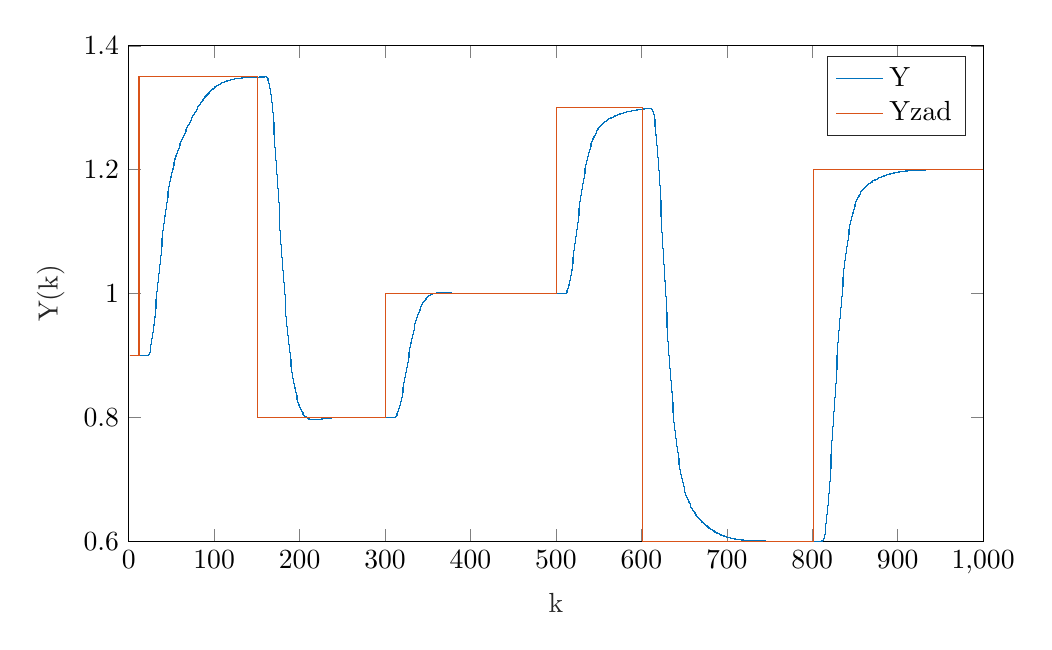
\begin{tikzpicture}

\begin{axis}[%
width=4.272in,
height=2.477in,
at={(0.717in,0.437in)},
scale only axis,
xmin=0,
xmax=1000,
xlabel style={font=\color{white!15!black}},
xlabel={k},
ymin=0.599992256828691,
ymax=1.4,
ylabel style={font=\color{white!15!black}},
ylabel={Y(k)},
axis background/.style={fill=white},
legend style={legend cell align=left, align=left, draw=white!15!black}
]
\addplot[const plot, color=mycolor1] table[row sep=crcr] {%
1	0.9\\
2	0.9\\
3	0.9\\
4	0.9\\
5	0.9\\
6	0.9\\
7	0.9\\
8	0.9\\
9	0.9\\
10	0.9\\
11	0.9\\
12	0.9\\
13	0.9\\
14	0.9\\
15	0.9\\
16	0.9\\
17	0.9\\
18	0.9\\
19	0.9\\
20	0.9\\
21	0.9\\
22	0.9003968325\\
23	0.90189871965075\\
24	0.905073306425321\\
25	0.910279490691062\\
26	0.917575470739387\\
27	0.926720028857513\\
28	0.937369034561701\\
29	0.949221897063396\\
30	0.962016762167375\\
31	0.975526203334917\\
32	0.98955335814073\\
33	1.00392211720768\\
34	1.01846532568581\\
35	1.03302365234678\\
36	1.04745021974169\\
37	1.06161385157993\\
38	1.07540137283722\\
39	1.08871898504561\\
40	1.10149268461784\\
41	1.11366781462215\\
42	1.12520790367634\\
43	1.13609297739469\\
44	1.14631754194966\\
45	1.1558884226304\\
46	1.164822596561\\
47	1.17314511477022\\
48	1.18088717545786\\
49	1.18808438530934\\
50	1.19477522725692\\
51	1.20099973972295\\
52	1.20679840295874\\
53	1.21221122169475\\
54	1.21727698922198\\
55	1.22203271565822\\
56	1.2265132020687\\
57	1.23075074195715\\
58	1.23477493214878\\
59	1.23861257604013\\
60	1.24228766343225\\
61	1.24582141257125\\
62	1.24923236150303\\
63	1.25253649734134\\
64	1.25574741350188\\
65	1.25887648633798\\
66	1.2619330639036\\
67	1.26492466075434\\
68	1.26785715377114\\
69	1.27073497495188\\
70	1.27356129796628\\
71	1.27633821601365\\
72	1.27906690916667\\
73	1.28174779993604\\
74	1.28438069625676\\
75	1.28696492148674\\
76	1.2894994313287\\
77	1.29198291784605\\
78	1.29441390094888\\
79	1.29679080788534\\
80	1.29911204139167\\
81	1.30137603723829\\
82	1.30358131196368\\
83	1.30572650161773\\
84	1.30781039234629\\
85	1.30983194364175\\
86	1.31179030506491\\
87	1.31368482721321\\
88	1.31551506767285\\
89	1.31728079264874\\
90	1.31898197491921\\
91	1.32061878871286\\
92	1.32219160205452\\
93	1.32370096707682\\
94	1.32514760874428\\
95	1.32653241238874\\
96	1.3278564104089\\
97	1.32912076844311\\
98	1.33032677128348\\
99	1.33147580876126\\
100	1.33256936179827\\
101	1.33360898878675\\
102	1.33459631243087\\
103	1.33553300715644\\
104	1.33642078717193\\
105	1.33726139524274\\
106	1.33805659222207\\
107	1.33880814736577\\
108	1.33951782944443\\
109	1.34018739865396\\
110	1.34081859931599\\
111	1.34141315335087\\
112	1.34197275449904\\
113	1.34249906326145\\
114	1.34299370252484\\
115	1.34345825383491\\
116	1.343894254278\\
117	1.34430319393038\\
118	1.34468651383366\\
119	1.34504560445459\\
120	1.34538180458811\\
121	1.34569640066303\\
122	1.34599062641116\\
123	1.34626566286218\\
124	1.34652263862785\\
125	1.34676263044158\\
126	1.34698666392079\\
127	1.34719571452181\\
128	1.34739070865921\\
129	1.34757252496318\\
130	1.3477419956511\\
131	1.34789990799113\\
132	1.34804700583764\\
133	1.34818399122054\\
134	1.34831152597188\\
135	1.34843023337525\\
136	1.34854069982486\\
137	1.34864347648302\\
138	1.34873908092574\\
139	1.34882799876802\\
140	1.3489106852612\\
141	1.3489875668561\\
142	1.34905904272676\\
143	1.34912548625032\\
144	1.34918724643967\\
145	1.34924464932612\\
146	1.34929799929011\\
147	1.34934758033859\\
148	1.34939365732814\\
149	1.34943647713367\\
150	1.34947626976246\\
151	1.34951324941425\\
152	1.34954761548793\\
153	1.34957955353586\\
154	1.34960923616711\\
155	1.34963682390087\\
156	1.34966246597171\\
157	1.34968630108823\\
158	1.34970845814693\\
159	1.34972905690297\\
160	1.34974820859986\\
161	1.34936918286629\\
162	1.34788385137995\\
163	1.34470057200117\\
164	1.33932997816735\\
165	1.33146241003619\\
166	1.32101534953336\\
167	1.30807213401816\\
168	1.29282864842148\\
169	1.27555247295626\\
170	1.25655193599623\\
171	1.23615301498745\\
172	1.21468242790329\\
173	1.1924555815405\\
174	1.16976830525739\\
175	1.14689151120634\\
176	1.12406809413145\\
177	1.10151152301675\\
178	1.07940568946233\\
179	1.05790566864792\\
180	1.03713912217916\\
181	1.01720813130079\\
182	0.998191296580753\\
183	0.980145978394943\\
184	0.963110583143162\\
185	0.947106824538888\\
186	0.932141908709745\\
187	0.918210607173271\\
188	0.905297193789104\\
189	0.893377231165183\\
190	0.882419199225688\\
191	0.872385964150951\\
192	0.863236090015963\\
193	0.854924998463032\\
194	0.84740598387186\\
195	0.840631092921057\\
196	0.834551878318362\\
197	0.829120036934084\\
198	0.824287942490576\\
199	0.820009083160094\\
200	0.816238414289025\\
201	0.812932635748424\\
202	0.810050402852148\\
203	0.807552479163711\\
204	0.805401838917962\\
205	0.803563726167765\\
206	0.802005677146285\\
207	0.800697511725418\\
208	0.799611299260059\\
209	0.798721303543281\\
210	0.798003911063929\\
211	0.797437546258748\\
212	0.797002576987652\\
213	0.796681213033688\\
214	0.7964574000387\\
215	0.796316710931004\\
216	0.796246236581258\\
217	0.796234477135434\\
218	0.796271235217511\\
219	0.796347511967148\\
220	0.796455406677302\\
221	0.796588020621207\\
222	0.796739365505593\\
223	0.796904276855286\\
224	0.797078332521593\\
225	0.797257776411233\\
226	0.797439447452308\\
227	0.797620713747221\\
228	0.797799411808039\\
229	0.797973790726109\\
230	0.798142461093451\\
231	0.798304348467379\\
232	0.798458651150783\\
233	0.798604802047644\\
234	0.798742434345614\\
235	0.798871350774182\\
236	0.798991496187271\\
237	0.799102933222456\\
238	0.799205820794793\\
239	0.799300395190978\\
240	0.79938695353881\\
241	0.799465839437325\\
242	0.799537430544174\\
243	0.799602127928504\\
244	0.799660347009677\\
245	0.799712509914225\\
246	0.799759039095511\\
247	0.799800352072391\\
248	0.799836857154686\\
249	0.799868950034413\\
250	0.799897011132346\\
251	0.799921403599647\\
252	0.799942471883861\\
253	0.799960540777604\\
254	0.799975914876708\\
255	0.79998887838241\\
256	0.799999695189495\\
257	0.80000860920895\\
258	0.800015844879908\\
259	0.800021607831247\\
260	0.800026085658369\\
261	0.800029448785317\\
262	0.800031851386598\\
263	0.800033432346852\\
264	0.800034316239898\\
265	0.800034614311675\\
266	0.800034425454304\\
267	0.800033837160833\\
268	0.800032926452305\\
269	0.800031760770607\\
270	0.800030398832129\\
271	0.800028891438614\\
272	0.800027282242739\\
273	0.800025608466986\\
274	0.800023901575144\\
275	0.800022187896526\\
276	0.800020489203528\\
277	0.800018823243618\\
278	0.800017204227237\\
279	0.800015643273347\\
280	0.800014148814597\\
281	0.800012726964214\\
282	0.800011381846846\\
283	0.800010115895608\\
284	0.800008930117633\\
285	0.800007824330387\\
286	0.800006797370981\\
287	0.800005847280665\\
288	0.800004971466573\\
289	0.800004166842753\\
290	0.800003429952374\\
291	0.800002757072925\\
292	0.800002144306098\\
293	0.800001587653944\\
294	0.80000108308279\\
295	0.800000626576271\\
296	0.800000214178762\\
297	0.799999842030353\\
298	0.79999950639444\\
299	0.799999203678905\\
300	0.799998930451752\\
301	0.799998683452009\\
302	0.799998459596597\\
303	0.799998255983831\\
304	0.799998069894104\\
305	0.79999789878829\\
306	0.799997740304308\\
307	0.799997592252251\\
308	0.799997452608449\\
309	0.799997319508765\\
310	0.799997191241407\\
311	0.800241735392682\\
312	0.801113642321269\\
313	0.802837703823257\\
314	0.805521829426677\\
315	0.80918919409615\\
316	0.813803279013992\\
317	0.819287229305482\\
318	0.825538678963042\\
319	0.832440971567669\\
320	0.839871525820564\\
321	0.847707949390355\\
322	0.855832386686442\\
323	0.864134490656075\\
324	0.872513331338063\\
325	0.880878491261607\\
326	0.889150547077852\\
327	0.897261095804212\\
328	0.905152450923259\\
329	0.912777106829552\\
330	0.920097048558929\\
331	0.927082966390048\\
332	0.933713420985021\\
333	0.93997399359084\\
334	0.945856446932517\\
335	0.951357915366188\\
336	0.956480137279462\\
337	0.961228738555811\\
338	0.965612572189216\\
339	0.969643116349326\\
340	0.97333393150609\\
341	0.976700175668096\\
342	0.979758175718789\\
343	0.98252505212167\\
344	0.985018393727433\\
345	0.987255979079745\\
346	0.989255540441178\\
347	0.991034566709301\\
348	0.992610141434867\\
349	0.993998812265234\\
350	0.995216488297129\\
351	0.996278362018223\\
352	0.997198852734453\\
353	0.997991568609958\\
354	0.998669284681483\\
355	0.999243934443288\\
356	0.999726612827774\\
357	1.00012758862783\\
358	1.00045632461725\\
359	1.00072150382355\\
360	1.00093106059283\\
361	1.00109221525735\\
362	1.00121151137455\\
363	1.00129485465003\\
364	1.00134755278781\\
365	1.00137435562928\\
366	1.00137949504798\\
367	1.00136672416173\\
368	1.00133935550725\\
369	1.00130029789613\\
370	1.00125209173533\\
371	1.00119694265174\\
372	1.00113675330826\\
373	1.0010731533406\\
374	1.00100752737901\\
375	1.00094104114841\\
376	1.00087466566531\\
377	1.00080919956929\\
378	1.00074528964342\\
379	1.00068344959024\\
380	1.0006240771397\\
381	1.00056746957229\\
382	1.00051383774569\\
383	1.0004633187156\\
384	1.00041598704315\\
385	1.00037186488101\\
386	1.00033093092891\\
387	1.0002931283476\\
388	1.00025837171704\\
389	1.00022655312151\\
390	1.00019754744038\\
391	1.00017121691934\\
392	1.00014741509233\\
393	1.00012599012026\\
394	1.00010678760816\\
395	1.00008965295776\\
396	1.00007443330832\\
397	1.00006097911446\\
398	1.0000491454052\\
399	1.00003879276512\\
400	1.00002978807419\\
401	1.00002200503991\\
402	1.0000153245515\\
403	1.0000096348834\\
404	1.00000483177185\\
405	1.00000081838606\\
406	0.99999750521293\\
407	0.999994809871851\\
408	0.999992656874277\\
409	0.999990977340686\\
410	0.999989708685961\\
411	0.999988794282603\\
412	0.999988183109847\\
413	0.999987829395475\\
414	0.999987692256029\\
415	0.99998773534014\\
416	0.999987926478823\\
417	0.999988237345811\\
418	0.999988643130359\\
419	0.999989122224347\\
420	0.999989655925025\\
421	0.999990228154303\\
422	0.999990825195146\\
423	0.999991435445298\\
424	0.999992049188323\\
425	0.999992658381745\\
426	0.999993256461879\\
427	0.999993838164825\\
428	0.999994399362979\\
429	0.999994936916357\\
430	0.99999544853795\\
431	0.999995932672294\\
432	0.999996388386443\\
433	0.999996815272482\\
434	0.999997213360775\\
435	0.999997583043112\\
436	0.999997925004963\\
437	0.999998240166073\\
438	0.999998529628667\\
439	0.999998794632549\\
440	0.999999036516452\\
441	0.999999256685005\\
442	0.99999945658073\\
443	0.999999637660548\\
444	0.999999801376259\\
445	0.999999949158561\\
446	1.00000008240417\\
447	1.00000020246564\\
448	1.00000031064357\\
449	1.00000040818078\\
450	1.00000049625831\\
451	1.00000057599286\\
452	1.00000064843543\\
453	1.00000071457106\\
454	1.0000007753194\\
455	1.0000008315359\\
456	1.00000088401361\\
457	1.00000093348531\\
458	1.00000098062596\\
459	1.00000102605533\\
460	1.00000107034068\\
461	1.00000111399953\\
462	1.00000115750233\\
463	1.000001201275\\
464	1.00000124570135\\
465	1.00000129112525\\
466	1.00000133785259\\
467	1.00000138615292\\
468	1.00000143626073\\
469	1.00000148837641\\
470	1.00000154266683\\
471	1.00000159926545\\
472	1.00000165827196\\
473	1.00000171975149\\
474	1.00000178373317\\
475	1.00000185020828\\
476	1.00000191912795\\
477	1.00000199040078\\
478	1.00000206389123\\
479	1.00000213941929\\
480	1.000002216762\\
481	1.00000229565665\\
482	1.00000237580565\\
483	1.00000245688255\\
484	1.0000025385389\\
485	1.00000262041156\\
486	1.00000270213008\\
487	1.00000278319374\\
488	1.00000286281258\\
489	1.00000293988318\\
490	1.00000301304141\\
491	1.0000030807532\\
492	1.00000314141751\\
493	1.00000319346569\\
494	1.00000323544788\\
495	1.00000326610191\\
496	1.0000032844033\\
497	1.00000328959677\\
498	1.00000328121129\\
499	1.00000325906065\\
500	1.00000322323261\\
501	1.00000317406898\\
502	1.00000311213917\\
503	1.00000303820955\\
504	1.0000029532103\\
505	1.0000028582016\\
506	1.00000275434024\\
507	1.00000264284782\\
508	1.00000252498109\\
509	1.00000240200517\\
510	1.00000227516978\\
511	1.00036914941852\\
512	1.00167706359427\\
513	1.0042632084337\\
514	1.00828945100859\\
515	1.01379055628457\\
516	1.02071174829612\\
517	1.02887713538837\\
518	1.03804444650837\\
519	1.04800021360269\\
520	1.05855890331387\\
521	1.06955978848347\\
522	1.08085647108788\\
523	1.09231017662515\\
524	1.10379282458815\\
525	1.11518905250805\\
526	1.12639728001237\\
527	1.13733012850774\\
528	1.14791446408807\\
529	1.15809112467692\\
530	1.16781431234489\\
531	1.17705068492311\\
532	1.1857782200559\\
533	1.1939849463973\\
534	1.20166762647908\\
535	1.20883045204209\\
536	1.21548379398338\\
537	1.22164303478199\\
538	1.22732750042129\\
539	1.23255950069934\\
540	1.23736348082907\\
541	1.24176528291098\\
542	1.2457915128404\\
543	1.24946900619178\\
544	1.25282438536875\\
545	1.255883699633\\
546	1.2586721393796\\
547	1.26121381609532\\
548	1.26353159972873\\
549	1.26564700564533\\
550	1.26758012388385\\
551	1.26934958402913\\
552	1.27097254964135\\
553	1.27246473680785\\
554	1.27384045199534\\
555	1.27511264496477\\
556	1.2762929730617\\
557	1.27739187370489\\
558	1.27841864236453\\
559	1.27938151374626\\
560	1.28028774427961\\
561	1.28114369434994\\
562	1.28195490901479\\
563	1.28272619620898\\
564	1.28346170167317\\
565	1.28416498003804\\
566	1.28483906166577\\
567	1.28548651499337\\
568	1.28610950424218\\
569	1.28670984245695\\
570	1.28728903991822\\
571	1.28784834803657\\
572	1.28838879888735\\
573	1.28891124058317\\
574	1.28941636870932\\
575	1.28990475406627\\
576	1.29037686697525\\
577	1.29083309840832\\
578	1.29127377820485\\
579	1.2916991906325\\
580	1.2921095875439\\
581	1.29250519937066\\
582	1.29288624418479\\
583	1.2932529350451\\
584	1.29360548583184\\
585	1.29394411575922\\
586	1.29426905274027\\
587	1.29458053576463\\
588	1.29487881643516\\
589	1.29516415979575\\
590	1.29543684456936\\
591	1.2956971629126\\
592	1.29594541978157\\
593	1.29618193199208\\
594	1.29640702704751\\
595	1.29662104179754\\
596	1.2968243209826\\
597	1.29701721571052\\
598	1.29720008190489\\
599	1.29737327875808\\
600	1.29753716721558\\
601	1.29769210851392\\
602	1.29783846278895\\
603	1.29797658776788\\
604	1.29810683755453\\
605	1.29822956151454\\
606	1.29834510326426\\
607	1.29845379976533\\
608	1.29855598052462\\
609	1.29865196689797\\
610	1.29874207149483\\
611	1.29842977956364\\
612	1.29700718753633\\
613	1.29388286886674\\
614	1.28856766346058\\
615	1.28066200813324\\
616	1.26984921614809\\
617	1.25598388738197\\
618	1.23913649491777\\
619	1.21965315589226\\
620	1.19804592254849\\
621	1.17478122285202\\
622	1.1502640294324\\
623	1.12484476260775\\
624	1.09884085778264\\
625	1.07255267534669\\
626	1.04625882038998\\
627	1.02021109143829\\
628	0.994631694549837\\
629	0.969712001324028\\
630	0.94561222790622\\
631	0.922461857317495\\
632	0.900360834800842\\
633	0.879381467674966\\
634	0.859570869769742\\
635	0.840953738559204\\
636	0.823535269022378\\
637	0.807304059265165\\
638	0.792234906886538\\
639	0.778291428794157\\
640	0.765428462794031\\
641	0.75359422850279\\
642	0.742732239327515\\
643	0.732782967522247\\
644	0.723685271537187\\
645	0.715377599724076\\
646	0.707798987504076\\
647	0.700889866782588\\
648	0.694592707056432\\
649	0.688852507575908\\
650	0.683617159311353\\
651	0.678837694497154\\
652	0.674468440313894\\
653	0.670467091919414\\
654	0.666794718625861\\
655	0.663415715597044\\
656	0.66029771204856\\
657	0.657411445600077\\
658	0.654730611173913\\
659	0.652231691668372\\
660	0.649893776564664\\
661	0.647698373654972\\
662	0.645629218205697\\
663	0.643672083091211\\
664	0.641814592745237\\
665	0.640046043173745\\
666	0.63835722974906\\
667	0.636740284053228\\
668	0.635188520653184\\
669	0.633696294364489\\
670	0.632258868288106\\
671	0.630872292680039\\
672	0.629533294531013\\
673	0.628239177587585\\
674	0.626987732432367\\
675	0.625777156155088\\
676	0.624605981084123\\
677	0.623473012006337\\
678	0.622377271278287\\
679	0.62131795122079\\
680	0.620294373188801\\
681	0.619305952717732\\
682	0.618352170164157\\
683	0.61743254628159\\
684	0.616546622199187\\
685	0.615693943301469\\
686	0.614874046539533\\
687	0.614086450542425\\
688	0.613330648268691\\
689	0.61260610208598\\
690	0.611912240857262\\
691	0.611248458672075\\
692	0.610614114912142\\
693	0.610008535384269\\
694	0.609431014291162\\
695	0.608880816843446\\
696	0.608357182344793\\
697	0.607859327607069\\
698	0.607386450574401\\
699	0.606937734054446\\
700	0.60651234947216\\
701	0.606109460576357\\
702	0.605728227042506\\
703	0.605367807926717\\
704	0.605027364935836\\
705	0.604706065487328\\
706	0.604403085540252\\
707	0.604117612185211\\
708	0.603848845986733\\
709	0.60359600307625\\
710	0.6033583169977\\
711	0.603135040310979\\
712	0.602925445961028\\
713	0.602728828422359\\
714	0.602544504630396\\
715	0.602371814712158\\
716	0.602210122529593\\
717	0.602058816049379\\
718	0.601917307553243\\
719	0.601785033702864\\
720	0.601661455473256\\
721	0.601546057968222\\
722	0.601438350131016\\
723	0.601337864362832\\
724	0.601244156061116\\
725	0.601156803089036\\
726	0.601075405186743\\
727	0.600999583334334\\
728	0.600928979075682\\
729	0.600863253811568\\
730	0.600802088069819\\
731	0.600745180759458\\
732	0.600692248415154\\
733	0.600643024437632\\
734	0.600597258335057\\
735	0.600554714969793\\
736	0.600515173814428\\
737	0.600478428220352\\
738	0.600444284701777\\
739	0.600412562237564\\
740	0.600383091592846\\
741	0.60035571466206\\
742	0.600330283834632\\
743	0.600306661384279\\
744	0.600284718882596\\
745	0.600264336637356\\
746	0.600245403155727\\
747	0.600227814632427\\
748	0.600211474462665\\
749	0.600196292779565\\
750	0.600182186015668\\
751	0.600169076487977\\
752	0.600156892005953\\
753	0.600145565501768\\
754	0.600135034682109\\
755	0.600125241700733\\
756	0.600116132851002\\
757	0.600107658277553\\
758	0.600099771706285\\
759	0.600092430191834\\
760	0.600085593881702\\
761	0.60007922579623\\
762	0.600073291623614\\
763	0.600067759529197\\
764	0.600062599978278\\
765	0.600057785571713\\
766	0.600053290893632\\
767	0.600049092370602\\
768	0.600045168141628\\
769	0.600041497938389\\
770	0.600038062975188\\
771	0.600034845848095\\
772	0.600031830442822\\
773	0.600029001850911\\
774	0.60002634629384\\
775	0.600023851054668\\
776	0.600021504416567\\
777	0.600019295607249\\
778	0.600017214747657\\
779	0.600015252802985\\
780	0.600013401534357\\
781	0.600011653449981\\
782	0.600010001755048\\
783	0.600008440300064\\
784	0.600006963527791\\
785	0.600005566419388\\
786	0.600004244440616\\
787	0.600002993700232\\
788	0.600001811214365\\
789	0.600000695014832\\
790	0.599999644148685\\
791	0.599998658605141\\
792	0.599997739194822\\
793	0.599996887349949\\
794	0.599996104847747\\
795	0.599995393520573\\
796	0.599994754991057\\
797	0.59999419045303\\
798	0.599993700507108\\
799	0.599993285051996\\
800	0.599992943227775\\
801	0.599992673404659\\
802	0.599992473209436\\
803	0.599992339581462\\
804	0.599992268850404\\
805	0.599992256828691\\
806	0.59999229891267\\
807	0.599992390187476\\
808	0.599992525531416\\
809	0.599992699716415\\
810	0.59999290750177\\
811	0.600389975648048\\
812	0.60189212049335\\
813	0.605091066460667\\
814	0.610476257022456\\
815	0.618418593506771\\
816	0.629096337849874\\
817	0.642482416159094\\
818	0.658404345011305\\
819	0.676500838047778\\
820	0.69632010754661\\
821	0.717469141219574\\
822	0.739607136686259\\
823	0.762430232727302\\
824	0.785655317067927\\
825	0.809018761579781\\
826	0.832281213717341\\
827	0.85523028994633\\
828	0.877681695053381\\
829	0.899479299397544\\
830	0.920494605595373\\
831	0.940625700625489\\
832	0.959795675272329\\
833	0.977950594447843\\
834	0.995057165910428\\
835	1.01110026499722\\
836	1.0260804411142\\
837	1.04001149501846\\
838	1.05291818757299\\
839	1.06483411894468\\
840	1.07579980077286\\
841	1.08586093155153\\
842	1.09506687645595\\
843	1.10346934639014\\
844	1.11112126656795\\
845	1.1180758220104\\
846	1.12438566558564\\
847	1.1301022733459\\
848	1.13527543170246\\
849	1.13995284124478\\
850	1.14417982261351\\
851	1.14799911067086\\
852	1.15145072418979\\
853	1.15457189934328\\
854	1.15739707636649\\
855	1.15995792985233\\
856	1.16228343419947\\
857	1.16439995674124\\
858	1.16633137203358\\
859	1.16809919166137\\
860	1.16972270473167\\
861	1.17121912495864\\
862	1.17260374090803\\
863	1.17389006656248\\
864	1.17508998989514\\
865	1.17621391760189\\
866	1.17727091454732\\
867	1.17826883682981\\
868	1.17921445767246\\
869	1.18011358560273\\
870	1.18097117460022\\
871	1.18179142607207\\
872	1.18257788266393\\
873	1.18333351403509\\
874	1.18406079482149\\
875	1.18476177508558\\
876	1.18543814360702\\
877	1.18609128440917\\
878	1.1867223269426\\
879	1.18733219036251\\
880	1.18792162234305\\
881	1.18849123287007\\
882	1.18904152344584\\
883	1.18957291212683\\
884	1.19008575479887\\
885	1.19058036307482\\
886	1.19105701917833\\
887	1.1915159881545\\
888	1.19195752772485\\
889	1.19238189608001\\
890	1.19278935788001\\
891	1.19318018870872\\
892	1.1935546782065\\
893	1.19391313208343\\
894	1.19425587319483\\
895	1.19458324184148\\
896	1.19489559543845\\
897	1.1951933076797\\
898	1.19547676730968\\
899	1.19574637659878\\
900	1.19600254960624\\
901	1.19624571030203\\
902	1.19647629060832\\
903	1.19669472841145\\
904	1.19690146558649\\
905	1.19709694606864\\
906	1.19728161399881\\
907	1.19745591196502\\
908	1.19762027935539\\
909	1.19777515083445\\
910	1.19792095495037\\
911	1.19805811287736\\
912	1.19818703729473\\
913	1.1983081314018\\
914	1.19842178806584\\
915	1.1985283890988\\
916	1.19862830465725\\
917	1.19872189275923\\
918	1.19880949891069\\
919	1.19889145583418\\
920	1.19896808329182\\
921	1.19903968799452\\
922	1.19910656358974\\
923	1.1991689907197\\
924	1.19922723714252\\
925	1.19928155790899\\
926	1.19933219558783\\
927	1.19937938053289\\
928	1.19942333118592\\
929	1.19946425440918\\
930	1.19950234584243\\
931	1.19953779027928\\
932	1.19957076205843\\
933	1.19960142546549\\
934	1.19962993514193\\
935	1.19965643649744\\
936	1.1996810661231\\
937	1.19970395220244\\
938	1.19972521491831\\
939	1.19974496685341\\
940	1.19976331338289\\
941	1.19978035305761\\
942	1.19979617797677\\
943	1.19981087414902\\
944	1.19982452184126\\
945	1.1998371959146\\
946	1.19984896614698\\
947	1.19985989754218\\
948	1.19987005062522\\
949	1.19987948172387\\
950	1.19988824323656\\
951	1.1998963838867\\
952	1.19990394896366\\
953	1.19991098055071\\
954	1.19991751774021\\
955	1.19992359683647\\
956	1.19992925154656\\
957	1.19993451315966\\
958	1.19993941071522\\
959	1.19994397116049\\
960	1.19994821949778\\
961	1.19995217892198\\
962	1.19995587094876\\
963	1.19995931553384\\
964	1.19996253118382\\
965	1.1999655350589\\
966	1.19996834306807\\
967	1.19997096995683\\
968	1.19997342938811\\
969	1.19997573401657\\
970	1.19997789555653\\
971	1.19997992484402\\
972	1.19998183189297\\
973	1.19998362594594\\
974	1.1999853155195\\
975	1.19998690844458\\
976	1.19998841190215\\
977	1.19998983245521\\
978	1.19999117607853\\
979	1.19999244818794\\
980	1.19999365367076\\
981	1.19999479691828\\
982	1.19999588186071\\
983	1.19999691200449\\
984	1.19999789047139\\
985	1.19999882003844\\
986	1.19999970317799\\
987	1.20000054188561\\
988	1.2000013374023\\
989	1.20000209009316\\
990	1.20000279943523\\
991	1.20000346409414\\
992	1.20000408210297\\
993	1.20000465111851\\
994	1.20000516869435\\
995	1.20000563253376\\
996	1.20000604070211\\
997	1.2000063917896\\
998	1.2000066850227\\
999	1.20000692032724\\
1000	1.20000709834866\\
};
\addlegendentry{Y}

\addplot[const plot, color=mycolor2] table[row sep=crcr] {%
1	0.9\\
2	0.9\\
3	0.9\\
4	0.9\\
5	0.9\\
6	0.9\\
7	0.9\\
8	0.9\\
9	0.9\\
10	0.9\\
11	0.9\\
12	1.35\\
13	1.35\\
14	1.35\\
15	1.35\\
16	1.35\\
17	1.35\\
18	1.35\\
19	1.35\\
20	1.35\\
21	1.35\\
22	1.35\\
23	1.35\\
24	1.35\\
25	1.35\\
26	1.35\\
27	1.35\\
28	1.35\\
29	1.35\\
30	1.35\\
31	1.35\\
32	1.35\\
33	1.35\\
34	1.35\\
35	1.35\\
36	1.35\\
37	1.35\\
38	1.35\\
39	1.35\\
40	1.35\\
41	1.35\\
42	1.35\\
43	1.35\\
44	1.35\\
45	1.35\\
46	1.35\\
47	1.35\\
48	1.35\\
49	1.35\\
50	1.35\\
51	1.35\\
52	1.35\\
53	1.35\\
54	1.35\\
55	1.35\\
56	1.35\\
57	1.35\\
58	1.35\\
59	1.35\\
60	1.35\\
61	1.35\\
62	1.35\\
63	1.35\\
64	1.35\\
65	1.35\\
66	1.35\\
67	1.35\\
68	1.35\\
69	1.35\\
70	1.35\\
71	1.35\\
72	1.35\\
73	1.35\\
74	1.35\\
75	1.35\\
76	1.35\\
77	1.35\\
78	1.35\\
79	1.35\\
80	1.35\\
81	1.35\\
82	1.35\\
83	1.35\\
84	1.35\\
85	1.35\\
86	1.35\\
87	1.35\\
88	1.35\\
89	1.35\\
90	1.35\\
91	1.35\\
92	1.35\\
93	1.35\\
94	1.35\\
95	1.35\\
96	1.35\\
97	1.35\\
98	1.35\\
99	1.35\\
100	1.35\\
101	1.35\\
102	1.35\\
103	1.35\\
104	1.35\\
105	1.35\\
106	1.35\\
107	1.35\\
108	1.35\\
109	1.35\\
110	1.35\\
111	1.35\\
112	1.35\\
113	1.35\\
114	1.35\\
115	1.35\\
116	1.35\\
117	1.35\\
118	1.35\\
119	1.35\\
120	1.35\\
121	1.35\\
122	1.35\\
123	1.35\\
124	1.35\\
125	1.35\\
126	1.35\\
127	1.35\\
128	1.35\\
129	1.35\\
130	1.35\\
131	1.35\\
132	1.35\\
133	1.35\\
134	1.35\\
135	1.35\\
136	1.35\\
137	1.35\\
138	1.35\\
139	1.35\\
140	1.35\\
141	1.35\\
142	1.35\\
143	1.35\\
144	1.35\\
145	1.35\\
146	1.35\\
147	1.35\\
148	1.35\\
149	1.35\\
150	1.35\\
151	0.8\\
152	0.8\\
153	0.8\\
154	0.8\\
155	0.8\\
156	0.8\\
157	0.8\\
158	0.8\\
159	0.8\\
160	0.8\\
161	0.8\\
162	0.8\\
163	0.8\\
164	0.8\\
165	0.8\\
166	0.8\\
167	0.8\\
168	0.8\\
169	0.8\\
170	0.8\\
171	0.8\\
172	0.8\\
173	0.8\\
174	0.8\\
175	0.8\\
176	0.8\\
177	0.8\\
178	0.8\\
179	0.8\\
180	0.8\\
181	0.8\\
182	0.8\\
183	0.8\\
184	0.8\\
185	0.8\\
186	0.8\\
187	0.8\\
188	0.8\\
189	0.8\\
190	0.8\\
191	0.8\\
192	0.8\\
193	0.8\\
194	0.8\\
195	0.8\\
196	0.8\\
197	0.8\\
198	0.8\\
199	0.8\\
200	0.8\\
201	0.8\\
202	0.8\\
203	0.8\\
204	0.8\\
205	0.8\\
206	0.8\\
207	0.8\\
208	0.8\\
209	0.8\\
210	0.8\\
211	0.8\\
212	0.8\\
213	0.8\\
214	0.8\\
215	0.8\\
216	0.8\\
217	0.8\\
218	0.8\\
219	0.8\\
220	0.8\\
221	0.8\\
222	0.8\\
223	0.8\\
224	0.8\\
225	0.8\\
226	0.8\\
227	0.8\\
228	0.8\\
229	0.8\\
230	0.8\\
231	0.8\\
232	0.8\\
233	0.8\\
234	0.8\\
235	0.8\\
236	0.8\\
237	0.8\\
238	0.8\\
239	0.8\\
240	0.8\\
241	0.8\\
242	0.8\\
243	0.8\\
244	0.8\\
245	0.8\\
246	0.8\\
247	0.8\\
248	0.8\\
249	0.8\\
250	0.8\\
251	0.8\\
252	0.8\\
253	0.8\\
254	0.8\\
255	0.8\\
256	0.8\\
257	0.8\\
258	0.8\\
259	0.8\\
260	0.8\\
261	0.8\\
262	0.8\\
263	0.8\\
264	0.8\\
265	0.8\\
266	0.8\\
267	0.8\\
268	0.8\\
269	0.8\\
270	0.8\\
271	0.8\\
272	0.8\\
273	0.8\\
274	0.8\\
275	0.8\\
276	0.8\\
277	0.8\\
278	0.8\\
279	0.8\\
280	0.8\\
281	0.8\\
282	0.8\\
283	0.8\\
284	0.8\\
285	0.8\\
286	0.8\\
287	0.8\\
288	0.8\\
289	0.8\\
290	0.8\\
291	0.8\\
292	0.8\\
293	0.8\\
294	0.8\\
295	0.8\\
296	0.8\\
297	0.8\\
298	0.8\\
299	0.8\\
300	0.8\\
301	1\\
302	1\\
303	1\\
304	1\\
305	1\\
306	1\\
307	1\\
308	1\\
309	1\\
310	1\\
311	1\\
312	1\\
313	1\\
314	1\\
315	1\\
316	1\\
317	1\\
318	1\\
319	1\\
320	1\\
321	1\\
322	1\\
323	1\\
324	1\\
325	1\\
326	1\\
327	1\\
328	1\\
329	1\\
330	1\\
331	1\\
332	1\\
333	1\\
334	1\\
335	1\\
336	1\\
337	1\\
338	1\\
339	1\\
340	1\\
341	1\\
342	1\\
343	1\\
344	1\\
345	1\\
346	1\\
347	1\\
348	1\\
349	1\\
350	1\\
351	1\\
352	1\\
353	1\\
354	1\\
355	1\\
356	1\\
357	1\\
358	1\\
359	1\\
360	1\\
361	1\\
362	1\\
363	1\\
364	1\\
365	1\\
366	1\\
367	1\\
368	1\\
369	1\\
370	1\\
371	1\\
372	1\\
373	1\\
374	1\\
375	1\\
376	1\\
377	1\\
378	1\\
379	1\\
380	1\\
381	1\\
382	1\\
383	1\\
384	1\\
385	1\\
386	1\\
387	1\\
388	1\\
389	1\\
390	1\\
391	1\\
392	1\\
393	1\\
394	1\\
395	1\\
396	1\\
397	1\\
398	1\\
399	1\\
400	1\\
401	1\\
402	1\\
403	1\\
404	1\\
405	1\\
406	1\\
407	1\\
408	1\\
409	1\\
410	1\\
411	1\\
412	1\\
413	1\\
414	1\\
415	1\\
416	1\\
417	1\\
418	1\\
419	1\\
420	1\\
421	1\\
422	1\\
423	1\\
424	1\\
425	1\\
426	1\\
427	1\\
428	1\\
429	1\\
430	1\\
431	1\\
432	1\\
433	1\\
434	1\\
435	1\\
436	1\\
437	1\\
438	1\\
439	1\\
440	1\\
441	1\\
442	1\\
443	1\\
444	1\\
445	1\\
446	1\\
447	1\\
448	1\\
449	1\\
450	1\\
451	1\\
452	1\\
453	1\\
454	1\\
455	1\\
456	1\\
457	1\\
458	1\\
459	1\\
460	1\\
461	1\\
462	1\\
463	1\\
464	1\\
465	1\\
466	1\\
467	1\\
468	1\\
469	1\\
470	1\\
471	1\\
472	1\\
473	1\\
474	1\\
475	1\\
476	1\\
477	1\\
478	1\\
479	1\\
480	1\\
481	1\\
482	1\\
483	1\\
484	1\\
485	1\\
486	1\\
487	1\\
488	1\\
489	1\\
490	1\\
491	1\\
492	1\\
493	1\\
494	1\\
495	1\\
496	1\\
497	1\\
498	1\\
499	1\\
500	1\\
501	1.3\\
502	1.3\\
503	1.3\\
504	1.3\\
505	1.3\\
506	1.3\\
507	1.3\\
508	1.3\\
509	1.3\\
510	1.3\\
511	1.3\\
512	1.3\\
513	1.3\\
514	1.3\\
515	1.3\\
516	1.3\\
517	1.3\\
518	1.3\\
519	1.3\\
520	1.3\\
521	1.3\\
522	1.3\\
523	1.3\\
524	1.3\\
525	1.3\\
526	1.3\\
527	1.3\\
528	1.3\\
529	1.3\\
530	1.3\\
531	1.3\\
532	1.3\\
533	1.3\\
534	1.3\\
535	1.3\\
536	1.3\\
537	1.3\\
538	1.3\\
539	1.3\\
540	1.3\\
541	1.3\\
542	1.3\\
543	1.3\\
544	1.3\\
545	1.3\\
546	1.3\\
547	1.3\\
548	1.3\\
549	1.3\\
550	1.3\\
551	1.3\\
552	1.3\\
553	1.3\\
554	1.3\\
555	1.3\\
556	1.3\\
557	1.3\\
558	1.3\\
559	1.3\\
560	1.3\\
561	1.3\\
562	1.3\\
563	1.3\\
564	1.3\\
565	1.3\\
566	1.3\\
567	1.3\\
568	1.3\\
569	1.3\\
570	1.3\\
571	1.3\\
572	1.3\\
573	1.3\\
574	1.3\\
575	1.3\\
576	1.3\\
577	1.3\\
578	1.3\\
579	1.3\\
580	1.3\\
581	1.3\\
582	1.3\\
583	1.3\\
584	1.3\\
585	1.3\\
586	1.3\\
587	1.3\\
588	1.3\\
589	1.3\\
590	1.3\\
591	1.3\\
592	1.3\\
593	1.3\\
594	1.3\\
595	1.3\\
596	1.3\\
597	1.3\\
598	1.3\\
599	1.3\\
600	1.3\\
601	0.6\\
602	0.6\\
603	0.6\\
604	0.6\\
605	0.6\\
606	0.6\\
607	0.6\\
608	0.6\\
609	0.6\\
610	0.6\\
611	0.6\\
612	0.6\\
613	0.6\\
614	0.6\\
615	0.6\\
616	0.6\\
617	0.6\\
618	0.6\\
619	0.6\\
620	0.6\\
621	0.6\\
622	0.6\\
623	0.6\\
624	0.6\\
625	0.6\\
626	0.6\\
627	0.6\\
628	0.6\\
629	0.6\\
630	0.6\\
631	0.6\\
632	0.6\\
633	0.6\\
634	0.6\\
635	0.6\\
636	0.6\\
637	0.6\\
638	0.6\\
639	0.6\\
640	0.6\\
641	0.6\\
642	0.6\\
643	0.6\\
644	0.6\\
645	0.6\\
646	0.6\\
647	0.6\\
648	0.6\\
649	0.6\\
650	0.6\\
651	0.6\\
652	0.6\\
653	0.6\\
654	0.6\\
655	0.6\\
656	0.6\\
657	0.6\\
658	0.6\\
659	0.6\\
660	0.6\\
661	0.6\\
662	0.6\\
663	0.6\\
664	0.6\\
665	0.6\\
666	0.6\\
667	0.6\\
668	0.6\\
669	0.6\\
670	0.6\\
671	0.6\\
672	0.6\\
673	0.6\\
674	0.6\\
675	0.6\\
676	0.6\\
677	0.6\\
678	0.6\\
679	0.6\\
680	0.6\\
681	0.6\\
682	0.6\\
683	0.6\\
684	0.6\\
685	0.6\\
686	0.6\\
687	0.6\\
688	0.6\\
689	0.6\\
690	0.6\\
691	0.6\\
692	0.6\\
693	0.6\\
694	0.6\\
695	0.6\\
696	0.6\\
697	0.6\\
698	0.6\\
699	0.6\\
700	0.6\\
701	0.6\\
702	0.6\\
703	0.6\\
704	0.6\\
705	0.6\\
706	0.6\\
707	0.6\\
708	0.6\\
709	0.6\\
710	0.6\\
711	0.6\\
712	0.6\\
713	0.6\\
714	0.6\\
715	0.6\\
716	0.6\\
717	0.6\\
718	0.6\\
719	0.6\\
720	0.6\\
721	0.6\\
722	0.6\\
723	0.6\\
724	0.6\\
725	0.6\\
726	0.6\\
727	0.6\\
728	0.6\\
729	0.6\\
730	0.6\\
731	0.6\\
732	0.6\\
733	0.6\\
734	0.6\\
735	0.6\\
736	0.6\\
737	0.6\\
738	0.6\\
739	0.6\\
740	0.6\\
741	0.6\\
742	0.6\\
743	0.6\\
744	0.6\\
745	0.6\\
746	0.6\\
747	0.6\\
748	0.6\\
749	0.6\\
750	0.6\\
751	0.6\\
752	0.6\\
753	0.6\\
754	0.6\\
755	0.6\\
756	0.6\\
757	0.6\\
758	0.6\\
759	0.6\\
760	0.6\\
761	0.6\\
762	0.6\\
763	0.6\\
764	0.6\\
765	0.6\\
766	0.6\\
767	0.6\\
768	0.6\\
769	0.6\\
770	0.6\\
771	0.6\\
772	0.6\\
773	0.6\\
774	0.6\\
775	0.6\\
776	0.6\\
777	0.6\\
778	0.6\\
779	0.6\\
780	0.6\\
781	0.6\\
782	0.6\\
783	0.6\\
784	0.6\\
785	0.6\\
786	0.6\\
787	0.6\\
788	0.6\\
789	0.6\\
790	0.6\\
791	0.6\\
792	0.6\\
793	0.6\\
794	0.6\\
795	0.6\\
796	0.6\\
797	0.6\\
798	0.6\\
799	0.6\\
800	0.6\\
801	1.2\\
802	1.2\\
803	1.2\\
804	1.2\\
805	1.2\\
806	1.2\\
807	1.2\\
808	1.2\\
809	1.2\\
810	1.2\\
811	1.2\\
812	1.2\\
813	1.2\\
814	1.2\\
815	1.2\\
816	1.2\\
817	1.2\\
818	1.2\\
819	1.2\\
820	1.2\\
821	1.2\\
822	1.2\\
823	1.2\\
824	1.2\\
825	1.2\\
826	1.2\\
827	1.2\\
828	1.2\\
829	1.2\\
830	1.2\\
831	1.2\\
832	1.2\\
833	1.2\\
834	1.2\\
835	1.2\\
836	1.2\\
837	1.2\\
838	1.2\\
839	1.2\\
840	1.2\\
841	1.2\\
842	1.2\\
843	1.2\\
844	1.2\\
845	1.2\\
846	1.2\\
847	1.2\\
848	1.2\\
849	1.2\\
850	1.2\\
851	1.2\\
852	1.2\\
853	1.2\\
854	1.2\\
855	1.2\\
856	1.2\\
857	1.2\\
858	1.2\\
859	1.2\\
860	1.2\\
861	1.2\\
862	1.2\\
863	1.2\\
864	1.2\\
865	1.2\\
866	1.2\\
867	1.2\\
868	1.2\\
869	1.2\\
870	1.2\\
871	1.2\\
872	1.2\\
873	1.2\\
874	1.2\\
875	1.2\\
876	1.2\\
877	1.2\\
878	1.2\\
879	1.2\\
880	1.2\\
881	1.2\\
882	1.2\\
883	1.2\\
884	1.2\\
885	1.2\\
886	1.2\\
887	1.2\\
888	1.2\\
889	1.2\\
890	1.2\\
891	1.2\\
892	1.2\\
893	1.2\\
894	1.2\\
895	1.2\\
896	1.2\\
897	1.2\\
898	1.2\\
899	1.2\\
900	1.2\\
901	1.2\\
902	1.2\\
903	1.2\\
904	1.2\\
905	1.2\\
906	1.2\\
907	1.2\\
908	1.2\\
909	1.2\\
910	1.2\\
911	1.2\\
912	1.2\\
913	1.2\\
914	1.2\\
915	1.2\\
916	1.2\\
917	1.2\\
918	1.2\\
919	1.2\\
920	1.2\\
921	1.2\\
922	1.2\\
923	1.2\\
924	1.2\\
925	1.2\\
926	1.2\\
927	1.2\\
928	1.2\\
929	1.2\\
930	1.2\\
931	1.2\\
932	1.2\\
933	1.2\\
934	1.2\\
935	1.2\\
936	1.2\\
937	1.2\\
938	1.2\\
939	1.2\\
940	1.2\\
941	1.2\\
942	1.2\\
943	1.2\\
944	1.2\\
945	1.2\\
946	1.2\\
947	1.2\\
948	1.2\\
949	1.2\\
950	1.2\\
951	1.2\\
952	1.2\\
953	1.2\\
954	1.2\\
955	1.2\\
956	1.2\\
957	1.2\\
958	1.2\\
959	1.2\\
960	1.2\\
961	1.2\\
962	1.2\\
963	1.2\\
964	1.2\\
965	1.2\\
966	1.2\\
967	1.2\\
968	1.2\\
969	1.2\\
970	1.2\\
971	1.2\\
972	1.2\\
973	1.2\\
974	1.2\\
975	1.2\\
976	1.2\\
977	1.2\\
978	1.2\\
979	1.2\\
980	1.2\\
981	1.2\\
982	1.2\\
983	1.2\\
984	1.2\\
985	1.2\\
986	1.2\\
987	1.2\\
988	1.2\\
989	1.2\\
990	1.2\\
991	1.2\\
992	1.2\\
993	1.2\\
994	1.2\\
995	1.2\\
996	1.2\\
997	1.2\\
998	1.2\\
999	1.2\\
1000	1.2\\
};
\addlegendentry{Yzad}

\end{axis}
\end{tikzpicture}%
\caption{Śledzenie wartości zadanej dla parametrów $N=200$, $N_u=5$,  $\lambda=15$}
\end{figure}

\begin{equation}
E = 36,4930
\end{equation}
\begin{equation}
E_{abs} = 90,6210
\end{equation}

Widzimy że regulacja jest troszkę gorsza.